\chapter{Testing of Massive IoT system} \label{ch:mass_test}
The focus of this chapter is to showcase the \gls{MDE} described in \autoref{ch:MassOver}. This is done in a series of test, where it is compared to the baseline emulator and to see if the changes made fulfills the goal set in \autoref{ch:MassOver}:

To emulate more than 15 devices, which do not interfere with each others workload and perform as well as the baseline emulator.


The test is done by comparing the \gls{MDE} to the baseline emulator, as well as testing the performance of the MDE at higher number of devices emulated.
The performance criteria that will be look into are:

\begin{itemize}
\item Error rate
\item Execution time
\item CPU usage
\item Memory usage
\end{itemize}

The error rate will showcase the stability of the MDE. This is done by starting the MDE multiple times and analyze the errors occurring. The errors can be analyzed from the log files.

The execution time is looked into to see if any processes in the MDE are taking longer, after the changes. This is measured by logging the time stamps, where the MDE goes from one step to another. 

CPU and memory usage is used to test for possible bottlenecks in the MDE. CPU usage is measured with the CPU stat tool, which can measure the CPU usage on the individual processes at a sample rate up to 3 Hz. The memory usage is measured using the top monitor tool, as all bigger buffers is allocated in the initialization and the used memory therefore is nearly static throughout the test. 

The parameters used for the eNB and SRS code is the default settings shown in \appref{app:Amarisoft} and \appref{app:SRSconfig}. The MDE are measured increasing the number of devices until the emulator hit 100\% in error rate multiple times in a row. Each point is measured 20 times. Besides testing the MDE, the baseline emulator is also tested, this is what the MDE is matched against. Note that baseline emulator can only emulate one device, the results will be extrapolated for comparison with multiple devices though.

\section{Error rate}
\label{sec:MTerror}
The error rate is analyzed from the log messages produces by the emulators. A successful run is defined by the emulator receiving msg2 in the NRAP, as this is as far as the baseline emulator is developed. These results can be seen on \autoref{fig:MT_error}.

\begin{figure}[H]
\tikzsetnextfilename{MT_error}
\centering
%\resizebox{0.5\textwidth}{!}{
% This file was created by matlab2tikz.
%
%The latest updates can be retrieved from
%  http://www.mathworks.com/matlabcentral/fileexchange/22022-matlab2tikz-matlab2tikz
%where you can also make suggestions and rate matlab2tikz.
%
\definecolor{mycolor1}{rgb}{0.00000,0.44700,0.74100}%
\definecolor{mycolor2}{rgb}{0.85000,0.32500,0.09800}%
%
\begin{tikzpicture}

\begin{axis}[%
width=4.521in,
height=3.566in,
at={(0.758in,0.481in)},
scale only axis,
xmin=1,
xmax=15,
xlabel={Number of UEs},
ymin=0,
ymax=100,
ylabel={Error rate (\%)},
axis background/.style={fill=white},
title style={font=\bfseries},
title={Error rate},
legend style={at={(0.03,0.97)},anchor=north west,legend cell align=left,align=left,draw=white!15!black}
]
\addplot [color=mycolor1,solid]
  table[row sep=crcr]{%
1	25\\
2	40\\
3	25\\
4	15\\
5	40\\
6	30\\
7	30\\
8	20\\
9	15\\
10	50\\
11	30\\
12	20\\
13	100\\
14	100\\
15	100\\
};
\addlegendentry{Change code};

\addplot [color=mycolor2,solid]
  table[row sep=crcr]{%
1	10\\
2	10\\
3	10\\
4	10\\
5	10\\
6	10\\
7	10\\
8	10\\
9	10\\
10	10\\
11	10\\
12	10\\
13	10\\
14	10\\
15	10\\
};
\addlegendentry{Baseline};

\end{axis}
\end{tikzpicture}%
\caption{Error rate for different number of devices.}
\label{fig:MT_error}
\end{figure}

As it can be seen on \autoref{fig:MT_error}, the error rate is higher for the MDE, than the baseline emulator. Another important aspect is that, when the number of devices hit 13, the error rate goes to 100\%, which shows the limit of the emulator. It should be noted that the process of monitoring and logging from the emulators might influence the outcome as up to 18 devices has been seen running on the MDE during the development. A more detailed overview of these errors, show that six different types of errors occur during the testing as shown on \autoref{fig:MT_error_dist}.

\begin{figure}[H]
\tikzsetnextfilename{MT_error_dist}
\centering
\resizebox{\textwidth}{!}{
% This file was created by matlab2tikz.
%
%The latest updates can be retrieved from
%  http://www.mathworks.com/matlabcentral/fileexchange/22022-matlab2tikz-matlab2tikz
%where you can also make suggestions and rate matlab2tikz.
%
\definecolor{mycolor1}{rgb}{0.20810,0.16630,0.52920}%
\definecolor{mycolor2}{rgb}{0.01651,0.42660,0.87863}%
\definecolor{mycolor3}{rgb}{0.02650,0.61370,0.81350}%
\definecolor{mycolor4}{rgb}{0.21783,0.72504,0.61926}%
\definecolor{mycolor5}{rgb}{0.64730,0.74560,0.41880}%
\definecolor{mycolor6}{rgb}{0.99377,0.74546,0.24035}%
\definecolor{mycolor7}{rgb}{0.97630,0.98310,0.05380}%
%
\begin{tikzpicture}

\begin{axis}[%
width=.8\textwidth,
height=.533\textwidth,
at={(0.533in,0.481in)},
scale only axis,
bar width=0.5,
xmin=-0.5,
xmax=15.5,
xtick={0,1,2,3,4,5,6,7,8,9,10,11,12,13,14,15},
xticklabels={{Base},{1},{2},{3},{4},{5},{6},{7},{8},{9},{10},{11},{12},{13},{14},{15}},
xlabel={Number of devices},
ymin=0,
ymax=100,
ylabel={Trials ($\%$)},
axis background/.style={fill=white},
title style={font=\bfseries},
title={Error distrubution},
legend style={at={(1.03,1)},anchor=north west,legend cell align=left,align=left,draw=white!15!black}
]
\addplot[ybar stacked,draw=black,fill=mycolor1,area legend] plot table[row sep=crcr] {%
0	90\\
1	75\\
2	60\\
3	75\\
4	85\\
5	60\\
6	70\\
7	70\\
8	80\\
9	85\\
10	50\\
11	70\\
12	80\\
13	0\\
14	0\\
15	0\\
};
\addlegendentry{No errors};

\addplot[ybar stacked,draw=black,fill=mycolor2,area legend] plot table[row sep=crcr] {%
0	0\\
1	0\\
2	0\\
3	0\\
4	0\\
5	0\\
6	0\\
7	0\\
8	5\\
9	0\\
10	0\\
11	0\\
12	0\\
13	5\\
14	0\\
15	0\\
};
\addlegendentry{Cell sync error};

\addplot[ybar stacked,draw=black,fill=mycolor3,area legend] plot table[row sep=crcr] {%
0	10\\
1	10\\
2	10\\
3	10\\
4	0\\
5	15\\
6	15\\
7	5\\
8	10\\
9	5\\
10	15\\
11	15\\
12	10\\
13	0\\
14	15\\
15	5\\
};
\addlegendentry{Radio error};

\addplot[ybar stacked,draw=black,fill=mycolor4,area legend] plot table[row sep=crcr] {%
0	0\\
1	10\\
2	30\\
3	15\\
4	15\\
5	25\\
6	10\\
7	25\\
8	5\\
9	5\\
10	30\\
11	5\\
12	5\\
13	80\\
14	65\\
15	60\\
};
\addlegendentry{Idle after MIB-NB};

\addplot[ybar stacked,draw=black,fill=mycolor5,area legend] plot table[row sep=crcr] {%
0	0\\
1	0\\
2	0\\
3	0\\
4	0\\
5	0\\
6	0\\
7	0\\
8	0\\
9	5\\
10	5\\
11	10\\
12	5\\
13	5\\
14	10\\
15	20\\
};
\addlegendentry{Transmission after NB-SIB1};

\addplot[ybar stacked,draw=black,fill=mycolor6,area legend] plot table[row sep=crcr] {%
0	0\\
1	0\\
2	0\\
3	0\\
4	0\\
5	0\\
6	5\\
7	0\\
8	0\\
9	0\\
10	0\\
11	0\\
12	0\\
13	10\\
14	10\\
15	10\\
};
\addlegendentry{NPRACH error};

\addplot[ybar stacked,draw=black,fill=mycolor7,area legend] plot table[row sep=crcr] 
\caption{The distribution of different errors for different number of devices.}
\label{fig:MT_error_dist}
\end{figure}

The \textit{Cell sync error} occurs when the emulator shuts down, before the device has synchronized to the cell and it goes to the MIB-NB step. This error is very rare, but as the error occurs so early in the process, these test runs will not give any data for any other step, beside initialization.

The \textit{radio error} comes from miscommunication between the radio class and the API for the USRP B210. It occurs when the process begins the search for NB-SIB1 message, where some radio parameters is changed. As the radio error is the only error occurring for the baseline emulator, this should be the only error, that is not produced by the changed made to the baseline emulator.

The \textit{idle after MIB-NB} error occur in the same part of the process as the radio error, where the emulator gets stuck and runs without retrying or closing down. This error type is the most frequently occurring among the errors produced by the changes to the emulator. An optimal place to improve the error rate, of the MDE, would be to look into the reason behind this error, especially for higher number of devices.


The \textit{transmission after NB-SIB1} is an error, that occurs at the NB-SIB1 step and the radio class transmit a signal, which causes the emulator to shut down. This error type have a tendency to occur with higher number of devices and can indicate a bottleneck in the process to get a higher number of devices.

The \textit{NPRACH error}, is an error that occurs, when some devices completes the NPRACH step, but other do not, as the system shuts down beforehand. This error type also have the tendency to occur at higher number of devices and likewise indicates a potential bottleneck.

The \textit{msg2 not received} error is when all devices have gone through the NPRACH step and are waiting on msg2, which is never received or not registered if received. This error is very rare and have no tendencies.

\section{Execution time}
\label{sec:exeTime}
To test the execution time for the emulator, the test is split up into the different steps of the code process discussed in \autoref{sub:MassStruct}.

\subsection{Initialization}
The execution time for the initialization step, is measured from the start of the MDE to the start of the cell seach step. The baseline emulator is measured as well, which gives the results seen on \autoref{fig:MT_Init_Time}.


\begin{figure}[H]
\tikzsetnextfilename{MT_Init_Time}
\centering
%\resizebox{0.7\textwidth}{!}{
% This file was created by matlab2tikz.
%
%The latest updates can be retrieved from
%  http://www.mathworks.com/matlabcentral/fileexchange/22022-matlab2tikz-matlab2tikz
%where you can also make suggestions and rate matlab2tikz.
%
\definecolor{mycolor1}{rgb}{0.00000,0.44700,0.74100}%
\definecolor{mycolor2}{rgb}{0.85000,0.32500,0.09800}%
%
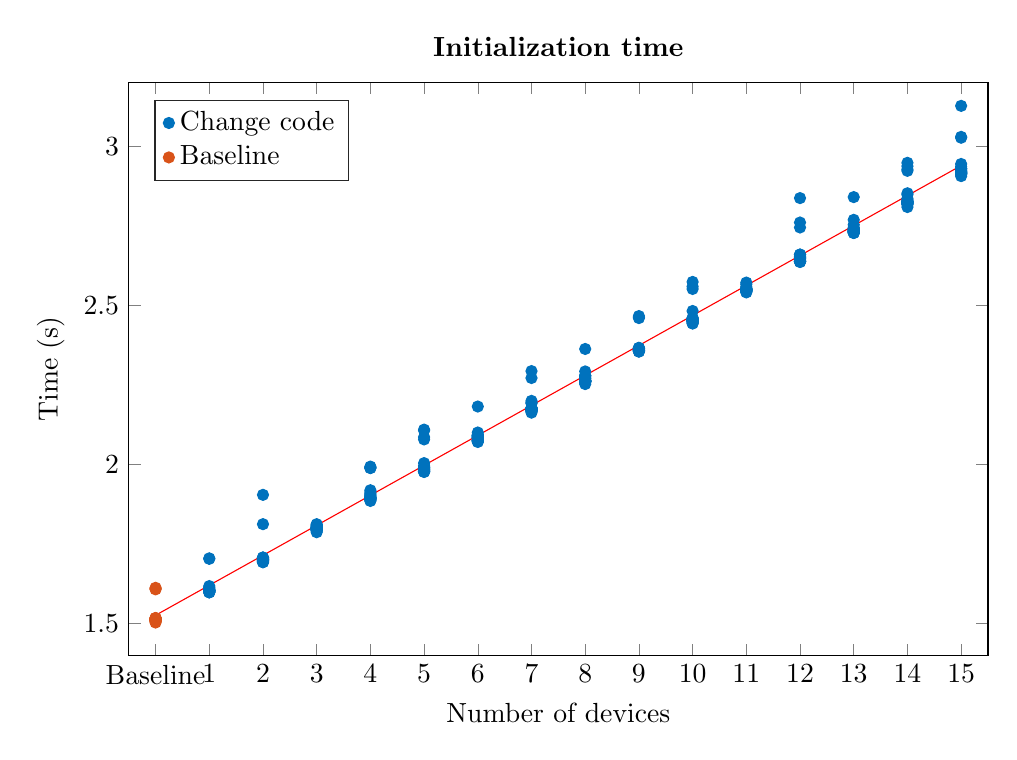
\begin{tikzpicture}

\begin{axis}[%
width=0.9\textwidth,
height=0.6\textwidth,
at={(0.758in,0.481in)},
scale only axis,
xmin=-0.5,
xmax=15.5,
xtick={0,1,2,3,4,5,6,7,8,9,10,11,12,13,14,15},
xticklabels={{Baseline},{1},{2},{3},{4},{5},{6},{7},{8},{9},{10},{11},{12},{13},{14},{15}},
xlabel={Number of devices},
ymin=1.4,
ymax=3.2,
ylabel={Time (s)},
axis background/.style={fill=white},
title style={font=\bfseries},
title={Initialization time},
legend style={at={(0.03,0.97)},anchor=north west,legend cell align=left,align=left,draw=white!15!black}
]



\addplot [color=mycolor1,only marks,mark=*,mark options={solid}]
  table[row sep=crcr]{%
1	1.60657000541687\\
1	1.60206508636475\\
1	1.60402417182922\\
1	1.60998201370239\\
1	1.59828901290894\\
1	1.59890818595886\\
1	1.60678696632385\\
1	1.70481204986572\\
1	1.60345387458801\\
1	1.59799599647522\\
1	1.60137987136841\\
1	1.60408782958984\\
1	1.60380721092224\\
1	1.61764979362488\\
1	1.61315512657166\\
1	1.60408186912537\\
1	1.60214781761169\\
1	1.59820103645325\\
1	1.70323586463928\\
1	1.60239100456238\\
};
\addlegendentry{Change code};

\addplot [color=mycolor2,only marks,mark=*,mark options={solid}]
  table[row sep=crcr]{%
0	1.51574110984802\\
0	1.60954785346985\\
0	1.61224007606506\\
0	1.51666712760925\\
0	1.51392078399658\\
0	1.51035499572754\\
0	1.50713300704956\\
0	1.51292109489441\\
0	1.51016092300415\\
0	1.5099790096283\\
0	1.51415991783142\\
0	1.51640319824219\\
0	1.51323890686035\\
0	1.51066589355469\\
0	1.5165901184082\\
0	1.50853300094604\\
0	1.50311899185181\\
0	1.60737919807434\\
0	1.51729917526245\\
0	1.50886988639832\\
};
\addlegendentry{Baseline};

\addplot [color=mycolor1,only marks,mark=*,mark options={solid},forget plot]
  table[row sep=crcr]{%
2	1.70376014709473\\
2	1.69752597808838\\
2	1.69991588592529\\
2	1.70224094390869\\
2	1.70335793495178\\
2	1.70019602775574\\
2	1.81223583221436\\
2	1.70259284973145\\
2	1.70058512687683\\
2	1.90431618690491\\
2	1.69746613502502\\
2	1.70056891441345\\
2	1.7057900428772\\
2	1.6926589012146\\
2	1.69660997390747\\
2	1.69284415245056\\
2	1.70735216140747\\
2	1.69585204124451\\
2	1.69405889511108\\
2	1.70744895935059\\
};


\addplot [color=mycolor1,only marks,mark=*,mark options={solid},forget plot]
  table[row sep=crcr]{%
3	1.79403805732727\\
3	1.80174088478088\\
3	1.80632400512695\\
3	1.79517197608948\\
3	1.7999119758606\\
3	1.80256199836731\\
3	1.79768395423889\\
3	1.79976677894592\\
3	1.79294800758362\\
3	1.80160784721375\\
3	1.81014108657837\\
3	1.8038489818573\\
3	1.79714298248291\\
3	1.78692388534546\\
3	1.80100011825562\\
3	1.79488515853882\\
3	1.81216788291931\\
3	1.79761385917664\\
3	1.80774402618408\\
3	1.79226994514465\\
};

\addplot [color=mycolor1,only marks,mark=*,mark options={solid},forget plot]
  table[row sep=crcr]{%
4	1.98840284347534\\
4	1.98891401290894\\
4	1.90781497955322\\
4	1.90410208702087\\
4	1.89322519302368\\
4	1.89481401443481\\
4	1.89260292053223\\
4	1.89337205886841\\
4	1.89051008224487\\
4	1.99312591552734\\
4	1.89608120918274\\
4	1.98998594284058\\
4	1.9188380241394\\
4	1.88647603988647\\
4	1.89477205276489\\
4	1.89825892448425\\
4	1.90163683891296\\
4	1.89038610458374\\
4	1.91325998306274\\
4	1.88523697853088\\
};
\addplot [color=mycolor1,only marks,mark=*,mark options={solid},forget plot]
  table[row sep=crcr]{%
5	1.99140405654907\\
5	1.98323607444763\\
5	2.10928916931152\\
5	1.97859597206116\\
5	2.08593010902405\\
5	1.97863793373108\\
5	1.99062418937683\\
5	2.07845187187195\\
5	1.99165511131287\\
5	1.97789597511292\\
5	1.98802804946899\\
5	1.9954240322113\\
5	2.00401997566223\\
5	1.98706889152527\\
5	1.98496317863464\\
5	1.97689509391785\\
5	1.98235487937927\\
5	1.98183512687683\\
5	2.10645198822021\\
5	1.97618389129639\\
};
\addplot [color=mycolor1,only marks,mark=*,mark options={solid},forget plot]
  table[row sep=crcr]{%
6	2.07043600082397\\
6	2.08795213699341\\
6	2.08343291282654\\
6	2.09298491477966\\
6	2.07702803611755\\
6	2.07426118850708\\
6	2.1002459526062\\
6	2.09029412269592\\
6	2.08507609367371\\
6	2.07489895820618\\
6	2.08115887641907\\
6	2.09077501296997\\
6	2.08771395683289\\
6	2.07395005226135\\
6	2.07281303405762\\
6	2.1818699836731\\
6	2.08554911613464\\
6	2.0755889415741\\
6	2.09108996391296\\
6	2.08529710769653\\
};
\addplot [color=mycolor1,only marks,mark=*,mark options={solid},forget plot]
  table[row sep=crcr]{%
7	2.16757988929749\\
7	2.16262793540955\\
7	2.17564296722412\\
7	2.1759250164032\\
7	2.19155502319336\\
7	2.27151203155518\\
7	2.1676127910614\\
7	2.17567276954651\\
7	2.17186117172241\\
7	2.29317903518677\\
7	2.17238211631775\\
7	2.17540311813354\\
7	2.17659687995911\\
7	2.16815400123596\\
7	2.17439103126526\\
7	2.17733693122864\\
7	2.17026114463806\\
7	2.17389607429504\\
7	2.19961309432983\\
7	2.1946439743042\\
};
\addplot [color=mycolor1,only marks,mark=*,mark options={solid},forget plot]
  table[row sep=crcr]{%
8	2.27100706100464\\
8	2.26513481140137\\
8	2.26285195350647\\
8	2.2616548538208\\
8	2.27730703353882\\
8	2.27119493484497\\
8	2.26165103912354\\
8	2.25236415863037\\
8	2.26101899147034\\
8	2.36273288726807\\
8	2.25905799865723\\
8	2.27876305580139\\
8	2.29212021827698\\
8	2.26190590858459\\
8	2.27887606620789\\
8	2.25859999656677\\
8	2.26044893264771\\
8	2.26256895065308\\
8	2.26363897323608\\
8	2.26199913024902\\
};
\addplot [color=mycolor1,only marks,mark=*,mark options={solid},forget plot]
  table[row sep=crcr]{%
9	2.35985803604126\\
9	2.35758590698242\\
9	2.35490608215332\\
9	2.35805201530457\\
9	2.35813903808594\\
9	2.36619591712952\\
9	2.36291694641113\\
9	2.3615140914917\\
9	2.36494493484497\\
9	2.35645508766174\\
9	2.36352205276489\\
9	2.36592721939087\\
9	2.46607184410095\\
9	2.46248698234558\\
9	2.35874915122986\\
9	2.35979104042053\\
9	2.36403608322144\\
9	2.35437083244324\\
9	2.45976400375366\\
9	2.35649704933167\\
};
\addplot [color=mycolor1,only marks,mark=*,mark options={solid},forget plot]
  table[row sep=crcr]{%
10	2.4522500038147\\
10	2.45602107048035\\
10	2.45017790794373\\
10	2.46005892753601\\
10	2.4437301158905\\
10	2.45332884788513\\
10	2.45075607299805\\
10	2.44673299789429\\
10	2.44251298904419\\
10	2.45762705802917\\
10	2.45294904708862\\
10	2.48201680183411\\
10	2.45067620277405\\
10	2.57340097427368\\
10	2.44935178756714\\
10	2.45021200180054\\
10	2.55899405479431\\
10	2.55124402046204\\
10	2.45972394943237\\
10	2.4552149772644\\
};
\addplot [color=mycolor1,only marks,mark=*,mark options={solid},forget plot]
  table[row sep=crcr]{%
11	2.54409885406494\\
11	2.5580689907074\\
11	2.55131316184998\\
11	2.54538011550903\\
11	2.54991102218628\\
11	2.54586219787598\\
11	2.54519009590149\\
11	2.54685091972351\\
11	2.54958415031433\\
11	2.55115580558777\\
11	2.55340099334717\\
11	2.54899501800537\\
11	2.54859089851379\\
11	2.55042195320129\\
11	2.54939794540405\\
11	2.57132411003113\\
11	2.54307293891907\\
11	2.54036903381348\\
11	2.54952502250671\\
11	2.56598615646362\\
};
\addplot [color=mycolor1,only marks,mark=*,mark options={solid},forget plot]
  table[row sep=crcr]{%
12	2.63736891746521\\
12	2.6386501789093\\
12	2.63579487800598\\
12	2.76004385948181\\
12	2.64884686470032\\
12	2.63978505134583\\
12	2.65288496017456\\
12	2.6491858959198\\
12	2.64470791816711\\
12	2.65107917785645\\
12	2.83676886558533\\
12	2.63889098167419\\
12	2.65938687324524\\
12	2.6382257938385\\
12	2.63785290718079\\
12	2.65852999687195\\
12	2.74441695213318\\
12	2.64707398414612\\
12	2.63858604431152\\
12	2.65901207923889\\
};
\addplot [color=mycolor1,only marks,mark=*,mark options={solid},forget plot]
  table[row sep=crcr]{%
13	2.73925495147705\\
13	2.76844787597656\\
13	2.74468803405762\\
13	2.72794198989868\\
13	2.73288083076477\\
13	2.72759079933167\\
13	2.73981499671936\\
13	2.73808693885803\\
13	2.73037505149841\\
13	2.73060989379883\\
13	2.75299692153931\\
13	2.73150610923767\\
13	2.73392391204834\\
13	2.83988189697266\\
13	2.73668503761292\\
13	2.73319101333618\\
13	2.7269880771637\\
13	2.73366594314575\\
13	2.73546814918518\\
13	2.73145604133606\\
};
\addplot [color=mycolor1,only marks,mark=*,mark options={solid},forget plot]
  table[row sep=crcr]{%
14	2.93708896636963\\
14	2.8230938911438\\
14	2.82491183280945\\
14	2.81724190711975\\
14	2.83096098899841\\
14	2.82523608207703\\
14	2.92713284492493\\
14	2.83528399467468\\
14	2.81740093231201\\
14	2.94761514663696\\
14	2.84746098518372\\
14	2.92244791984558\\
14	2.82092189788818\\
14	2.82772517204285\\
14	2.82116103172302\\
14	2.8086531162262\\
14	2.82523202896118\\
14	2.82433700561523\\
14	2.85196495056152\\
14	2.82061409950256\\
};
\addplot [color=mycolor1,only marks,mark=*,mark options={solid},forget plot]
  table[row sep=crcr]{%
15	2.91355895996094\\
15	2.92956900596619\\
15	2.92799687385559\\
15	3.0291600227356\\
15	2.92018890380859\\
15	2.92904806137085\\
15	2.91579508781433\\
15	2.91569089889526\\
15	2.92359805107117\\
15	2.91793894767761\\
15	2.9355640411377\\
15	3.12653303146362\\
15	2.91362810134888\\
15	2.94397902488709\\
15	2.9135410785675\\
15	2.91744613647461\\
15	2.92062401771545\\
15	2.91158103942871\\
15	3.02637410163879\\
15	2.90584707260132\\
};

\addplot [color=red,solid,forget plot]
  table[row sep=crcr]{%
0	1.52591009015129\\
0.015	1.52732309482467\\
0.03	1.52873609949805\\
0.045	1.53014910417142\\
0.06	1.5315621088448\\
0.075	1.53297511351818\\
0.09	1.53438811819156\\
0.105	1.53580112286494\\
0.12	1.53721412753832\\
0.135	1.5386271322117\\
0.15	1.54004013688508\\
0.165	1.54145314155845\\
0.18	1.54286614623183\\
0.195	1.54427915090521\\
0.21	1.54569215557859\\
0.225	1.54710516025197\\
0.24	1.54851816492535\\
0.255	1.54993116959873\\
0.27	1.55134417427211\\
0.285	1.55275717894549\\
0.3	1.55417018361886\\
0.315	1.55558318829224\\
0.33	1.55699619296562\\
0.345	1.558409197639\\
0.36	1.55982220231238\\
0.375	1.56123520698576\\
0.39	1.56264821165914\\
0.405	1.56406121633252\\
0.42	1.56547422100589\\
0.435	1.56688722567927\\
0.45	1.56830023035265\\
0.465	1.56971323502603\\
0.48	1.57112623969941\\
0.495	1.57253924437279\\
0.51	1.57395224904617\\
0.525	1.57536525371955\\
0.54	1.57677825839293\\
0.555	1.5781912630663\\
0.57	1.57960426773968\\
0.585	1.58101727241306\\
0.6	1.58243027708644\\
0.615	1.58384328175982\\
0.63	1.5852562864332\\
0.645	1.58666929110658\\
0.66	1.58808229577996\\
0.675	1.58949530045333\\
0.69	1.59090830512671\\
0.705	1.59232130980009\\
0.72	1.59373431447347\\
0.735	1.59514731914685\\
0.75	1.59656032382023\\
0.765	1.59797332849361\\
0.78	1.59938633316699\\
0.795	1.60079933784036\\
0.81	1.60221234251374\\
0.825	1.60362534718712\\
0.84	1.6050383518605\\
0.855	1.60645135653388\\
0.87	1.60786436120726\\
0.885	1.60927736588064\\
0.9	1.61069037055402\\
0.915	1.6121033752274\\
0.93	1.61351637990077\\
0.945	1.61492938457415\\
0.96	1.61634238924753\\
0.975	1.61775539392091\\
0.99	1.61916839859429\\
1.005	1.62058140326767\\
1.02	1.62199440794105\\
1.035	1.62340741261443\\
1.05	1.6248204172878\\
1.065	1.62623342196118\\
1.08	1.62764642663456\\
1.095	1.62905943130794\\
1.11	1.63047243598132\\
1.125	1.6318854406547\\
1.14	1.63329844532808\\
1.155	1.63471145000146\\
1.17	1.63612445467484\\
1.185	1.63753745934821\\
1.2	1.63895046402159\\
1.215	1.64036346869497\\
1.23	1.64177647336835\\
1.245	1.64318947804173\\
1.26	1.64460248271511\\
1.275	1.64601548738849\\
1.29	1.64742849206187\\
1.305	1.64884149673524\\
1.32	1.65025450140862\\
1.335	1.651667506082\\
1.35	1.65308051075538\\
1.365	1.65449351542876\\
1.38	1.65590652010214\\
1.395	1.65731952477552\\
1.41	1.6587325294489\\
1.425	1.66014553412227\\
1.44	1.66155853879565\\
1.455	1.66297154346903\\
1.47	1.66438454814241\\
1.485	1.66579755281579\\
1.5	1.66721055748917\\
1.515	1.66862356216255\\
1.53	1.67003656683593\\
1.545	1.67144957150931\\
1.56	1.67286257618268\\
1.575	1.67427558085606\\
1.59	1.67568858552944\\
1.605	1.67710159020282\\
1.62	1.6785145948762\\
1.635	1.67992759954958\\
1.65	1.68134060422296\\
1.665	1.68275360889634\\
1.68	1.68416661356971\\
1.695	1.68557961824309\\
1.71	1.68699262291647\\
1.725	1.68840562758985\\
1.74	1.68981863226323\\
1.755	1.69123163693661\\
1.77	1.69264464160999\\
1.785	1.69405764628337\\
1.8	1.69547065095674\\
1.815	1.69688365563012\\
1.83	1.6982966603035\\
1.845	1.69970966497688\\
1.86	1.70112266965026\\
1.875	1.70253567432364\\
1.89	1.70394867899702\\
1.905	1.7053616836704\\
1.92	1.70677468834378\\
1.935	1.70818769301715\\
1.95	1.70960069769053\\
1.965	1.71101370236391\\
1.98	1.71242670703729\\
1.995	1.71383971171067\\
2.01	1.71525271638405\\
2.025	1.71666572105743\\
2.04	1.71807872573081\\
2.055	1.71949173040418\\
2.07	1.72090473507756\\
2.085	1.72231773975094\\
2.1	1.72373074442432\\
2.115	1.7251437490977\\
2.13	1.72655675377108\\
2.145	1.72796975844446\\
2.16	1.72938276311784\\
2.175	1.73079576779121\\
2.19	1.73220877246459\\
2.205	1.73362177713797\\
2.22	1.73503478181135\\
2.235	1.73644778648473\\
2.25	1.73786079115811\\
2.265	1.73927379583149\\
2.28	1.74068680050487\\
2.295	1.74209980517825\\
2.31	1.74351280985162\\
2.325	1.744925814525\\
2.34	1.74633881919838\\
2.355	1.74775182387176\\
2.37	1.74916482854514\\
2.385	1.75057783321852\\
2.4	1.7519908378919\\
2.415	1.75340384256528\\
2.43	1.75481684723865\\
2.445	1.75622985191203\\
2.46	1.75764285658541\\
2.475	1.75905586125879\\
2.49	1.76046886593217\\
2.505	1.76188187060555\\
2.52	1.76329487527893\\
2.535	1.76470787995231\\
2.55	1.76612088462569\\
2.565	1.76753388929906\\
2.58	1.76894689397244\\
2.595	1.77035989864582\\
2.61	1.7717729033192\\
2.625	1.77318590799258\\
2.64	1.77459891266596\\
2.655	1.77601191733934\\
2.67	1.77742492201272\\
2.685	1.77883792668609\\
2.7	1.78025093135947\\
2.715	1.78166393603285\\
2.73	1.78307694070623\\
2.745	1.78448994537961\\
2.76	1.78590295005299\\
2.775	1.78731595472637\\
2.79	1.78872895939975\\
2.805	1.79014196407312\\
2.82	1.7915549687465\\
2.835	1.79296797341988\\
2.85	1.79438097809326\\
2.865	1.79579398276664\\
2.88	1.79720698744002\\
2.895	1.7986199921134\\
2.91	1.80003299678678\\
2.925	1.80144600146016\\
2.94	1.80285900613353\\
2.955	1.80427201080691\\
2.97	1.80568501548029\\
2.985	1.80709802015367\\
3	1.80851102482705\\
3.015	1.80992402950043\\
3.03	1.81133703417381\\
3.045	1.81275003884719\\
3.06	1.81416304352056\\
3.075	1.81557604819394\\
3.09	1.81698905286732\\
3.105	1.8184020575407\\
3.12	1.81981506221408\\
3.135	1.82122806688746\\
3.15	1.82264107156084\\
3.165	1.82405407623422\\
3.18	1.8254670809076\\
3.195	1.82688008558097\\
3.21	1.82829309025435\\
3.225	1.82970609492773\\
3.24	1.83111909960111\\
3.255	1.83253210427449\\
3.27	1.83394510894787\\
3.285	1.83535811362125\\
3.3	1.83677111829463\\
3.315	1.838184122968\\
3.33	1.83959712764138\\
3.345	1.84101013231476\\
3.36	1.84242313698814\\
3.375	1.84383614166152\\
3.39	1.8452491463349\\
3.405	1.84666215100828\\
3.42	1.84807515568166\\
3.435	1.84948816035503\\
3.45	1.85090116502841\\
3.465	1.85231416970179\\
3.48	1.85372717437517\\
3.495	1.85514017904855\\
3.51	1.85655318372193\\
3.525	1.85796618839531\\
3.54	1.85937919306869\\
3.555	1.86079219774207\\
3.57	1.86220520241544\\
3.585	1.86361820708882\\
3.6	1.8650312117622\\
3.615	1.86644421643558\\
3.63	1.86785722110896\\
3.645	1.86927022578234\\
3.66	1.87068323045572\\
3.675	1.8720962351291\\
3.69	1.87350923980247\\
3.705	1.87492224447585\\
3.72	1.87633524914923\\
3.735	1.87774825382261\\
3.75	1.87916125849599\\
3.765	1.88057426316937\\
3.78	1.88198726784275\\
3.795	1.88340027251613\\
3.81	1.88481327718951\\
3.825	1.88622628186288\\
3.84	1.88763928653626\\
3.855	1.88905229120964\\
3.87	1.89046529588302\\
3.885	1.8918783005564\\
3.9	1.89329130522978\\
3.915	1.89470430990316\\
3.93	1.89611731457654\\
3.945	1.89753031924991\\
3.96	1.89894332392329\\
3.975	1.90035632859667\\
3.99	1.90176933327005\\
4.005	1.90318233794343\\
4.02	1.90459534261681\\
4.035	1.90600834729019\\
4.05	1.90742135196357\\
4.065	1.90883435663694\\
4.08	1.91024736131032\\
4.095	1.9116603659837\\
4.11	1.91307337065708\\
4.125	1.91448637533046\\
4.14	1.91589938000384\\
4.155	1.91731238467722\\
4.17	1.9187253893506\\
4.185	1.92013839402397\\
4.2	1.92155139869735\\
4.215	1.92296440337073\\
4.23	1.92437740804411\\
4.245	1.92579041271749\\
4.26	1.92720341739087\\
4.275	1.92861642206425\\
4.29	1.93002942673763\\
4.305	1.93144243141101\\
4.32	1.93285543608438\\
4.335	1.93426844075776\\
4.35	1.93568144543114\\
4.365	1.93709445010452\\
4.38	1.9385074547779\\
4.395	1.93992045945128\\
4.41	1.94133346412466\\
4.425	1.94274646879804\\
4.44	1.94415947347141\\
4.455	1.94557247814479\\
4.47	1.94698548281817\\
4.485	1.94839848749155\\
4.5	1.94981149216493\\
4.515	1.95122449683831\\
4.53	1.95263750151169\\
4.545	1.95405050618507\\
4.56	1.95546351085845\\
4.575	1.95687651553182\\
4.59	1.9582895202052\\
4.605	1.95970252487858\\
4.62	1.96111552955196\\
4.635	1.96252853422534\\
4.65	1.96394153889872\\
4.665	1.9653545435721\\
4.68	1.96676754824548\\
4.695	1.96818055291885\\
4.71	1.96959355759223\\
4.725	1.97100656226561\\
4.74	1.97241956693899\\
4.755	1.97383257161237\\
4.77	1.97524557628575\\
4.785	1.97665858095913\\
4.8	1.97807158563251\\
4.815	1.97948459030588\\
4.83	1.98089759497926\\
4.845	1.98231059965264\\
4.86	1.98372360432602\\
4.875	1.9851366089994\\
4.89	1.98654961367278\\
4.905	1.98796261834616\\
4.92	1.98937562301954\\
4.935	1.99078862769292\\
4.95	1.99220163236629\\
4.965	1.99361463703967\\
4.98	1.99502764171305\\
4.995	1.99644064638643\\
5.01	1.99785365105981\\
5.025	1.99926665573319\\
5.04	2.00067966040657\\
5.055	2.00209266507995\\
5.07	2.00350566975332\\
5.085	2.0049186744267\\
5.1	2.00633167910008\\
5.115	2.00774468377346\\
5.13	2.00915768844684\\
5.145	2.01057069312022\\
5.16	2.0119836977936\\
5.175	2.01339670246698\\
5.19	2.01480970714035\\
5.205	2.01622271181373\\
5.22	2.01763571648711\\
5.235	2.01904872116049\\
5.25	2.02046172583387\\
5.265	2.02187473050725\\
5.28	2.02328773518063\\
5.295	2.02470073985401\\
5.31	2.02611374452739\\
5.325	2.02752674920076\\
5.34	2.02893975387414\\
5.355	2.03035275854752\\
5.37	2.0317657632209\\
5.385	2.03317876789428\\
5.4	2.03459177256766\\
5.415	2.03600477724104\\
5.43	2.03741778191442\\
5.445	2.03883078658779\\
5.46	2.04024379126117\\
5.475	2.04165679593455\\
5.49	2.04306980060793\\
5.505	2.04448280528131\\
5.52	2.04589580995469\\
5.535	2.04730881462807\\
5.55	2.04872181930145\\
5.565	2.05013482397483\\
5.58	2.0515478286482\\
5.595	2.05296083332158\\
5.61	2.05437383799496\\
5.625	2.05578684266834\\
5.64	2.05719984734172\\
5.655	2.0586128520151\\
5.67	2.06002585668848\\
5.685	2.06143886136186\\
5.7	2.06285186603523\\
5.715	2.06426487070861\\
5.73	2.06567787538199\\
5.745	2.06709088005537\\
5.76	2.06850388472875\\
5.775	2.06991688940213\\
5.79	2.07132989407551\\
5.805	2.07274289874889\\
5.82	2.07415590342226\\
5.835	2.07556890809564\\
5.85	2.07698191276902\\
5.865	2.0783949174424\\
5.88	2.07980792211578\\
5.895	2.08122092678916\\
5.91	2.08263393146254\\
5.925	2.08404693613592\\
5.94	2.0854599408093\\
5.955	2.08687294548267\\
5.97	2.08828595015605\\
5.985	2.08969895482943\\
6	2.09111195950281\\
6.015	2.09252496417619\\
6.03	2.09393796884957\\
6.045	2.09535097352295\\
6.06	2.09676397819633\\
6.075	2.0981769828697\\
6.09	2.09958998754308\\
6.105	2.10100299221646\\
6.12	2.10241599688984\\
6.135	2.10382900156322\\
6.15	2.1052420062366\\
6.165	2.10665501090998\\
6.18	2.10806801558336\\
6.195	2.10948102025674\\
6.21	2.11089402493011\\
6.225	2.11230702960349\\
6.24	2.11372003427687\\
6.255	2.11513303895025\\
6.27	2.11654604362363\\
6.285	2.11795904829701\\
6.3	2.11937205297039\\
6.315	2.12078505764377\\
6.33	2.12219806231714\\
6.345	2.12361106699052\\
6.36	2.1250240716639\\
6.375	2.12643707633728\\
6.39	2.12785008101066\\
6.405	2.12926308568404\\
6.42	2.13067609035742\\
6.435	2.1320890950308\\
6.45	2.13350209970417\\
6.465	2.13491510437755\\
6.48	2.13632810905093\\
6.495	2.13774111372431\\
6.51	2.13915411839769\\
6.525	2.14056712307107\\
6.54	2.14198012774445\\
6.555	2.14339313241783\\
6.57	2.14480613709121\\
6.585	2.14621914176458\\
6.6	2.14763214643796\\
6.615	2.14904515111134\\
6.63	2.15045815578472\\
6.645	2.1518711604581\\
6.66	2.15328416513148\\
6.675	2.15469716980486\\
6.69	2.15611017447824\\
6.705	2.15752317915161\\
6.72	2.15893618382499\\
6.735	2.16034918849837\\
6.75	2.16176219317175\\
6.765	2.16317519784513\\
6.78	2.16458820251851\\
6.795	2.16600120719189\\
6.81	2.16741421186527\\
6.825	2.16882721653865\\
6.84	2.17024022121202\\
6.855	2.1716532258854\\
6.87	2.17306623055878\\
6.885	2.17447923523216\\
6.9	2.17589223990554\\
6.915	2.17730524457892\\
6.93	2.1787182492523\\
6.945	2.18013125392568\\
6.96	2.18154425859905\\
6.975	2.18295726327243\\
6.99	2.18437026794581\\
7.005	2.18578327261919\\
7.02	2.18719627729257\\
7.035	2.18860928196595\\
7.05	2.19002228663933\\
7.065	2.19143529131271\\
7.08	2.19284829598608\\
7.095	2.19426130065946\\
7.11	2.19567430533284\\
7.125	2.19708731000622\\
7.14	2.1985003146796\\
7.155	2.19991331935298\\
7.17	2.20132632402636\\
7.185	2.20273932869974\\
7.2	2.20415233337312\\
7.215	2.20556533804649\\
7.23	2.20697834271987\\
7.245	2.20839134739325\\
7.26	2.20980435206663\\
7.275	2.21121735674001\\
7.29	2.21263036141339\\
7.305	2.21404336608677\\
7.32	2.21545637076015\\
7.335	2.21686937543352\\
7.35	2.2182823801069\\
7.365	2.21969538478028\\
7.38	2.22110838945366\\
7.395	2.22252139412704\\
7.41	2.22393439880042\\
7.425	2.2253474034738\\
7.44	2.22676040814718\\
7.455	2.22817341282055\\
7.47	2.22958641749393\\
7.485	2.23099942216731\\
7.5	2.23241242684069\\
7.515	2.23382543151407\\
7.53	2.23523843618745\\
7.545	2.23665144086083\\
7.56	2.23806444553421\\
7.575	2.23947745020759\\
7.59	2.24089045488096\\
7.605	2.24230345955434\\
7.62	2.24371646422772\\
7.635	2.2451294689011\\
7.65	2.24654247357448\\
7.665	2.24795547824786\\
7.68	2.24936848292124\\
7.695	2.25078148759462\\
7.71	2.25219449226799\\
7.725	2.25360749694137\\
7.74	2.25502050161475\\
7.755	2.25643350628813\\
7.77	2.25784651096151\\
7.785	2.25925951563489\\
7.8	2.26067252030827\\
7.815	2.26208552498165\\
7.83	2.26349852965503\\
7.845	2.2649115343284\\
7.86	2.26632453900178\\
7.875	2.26773754367516\\
7.89	2.26915054834854\\
7.905	2.27056355302192\\
7.92	2.2719765576953\\
7.935	2.27338956236868\\
7.95	2.27480256704206\\
7.965	2.27621557171543\\
7.98	2.27762857638881\\
7.995	2.27904158106219\\
8.01	2.28045458573557\\
8.025	2.28186759040895\\
8.04	2.28328059508233\\
8.055	2.28469359975571\\
8.07	2.28610660442909\\
8.085	2.28751960910246\\
8.1	2.28893261377584\\
8.115	2.29034561844922\\
8.13	2.2917586231226\\
8.145	2.29317162779598\\
8.16	2.29458463246936\\
8.175	2.29599763714274\\
8.19	2.29741064181612\\
8.205	2.2988236464895\\
8.22	2.30023665116287\\
8.235	2.30164965583625\\
8.25	2.30306266050963\\
8.265	2.30447566518301\\
8.28	2.30588866985639\\
8.295	2.30730167452977\\
8.31	2.30871467920315\\
8.325	2.31012768387653\\
8.34	2.3115406885499\\
8.355	2.31295369322328\\
8.37	2.31436669789666\\
8.385	2.31577970257004\\
8.4	2.31719270724342\\
8.415	2.3186057119168\\
8.43	2.32001871659018\\
8.445	2.32143172126356\\
8.46	2.32284472593693\\
8.475	2.32425773061031\\
8.49	2.32567073528369\\
8.505	2.32708373995707\\
8.52	2.32849674463045\\
8.535	2.32990974930383\\
8.55	2.33132275397721\\
8.565	2.33273575865059\\
8.58	2.33414876332397\\
8.595	2.33556176799734\\
8.61	2.33697477267072\\
8.625	2.3383877773441\\
8.64	2.33980078201748\\
8.655	2.34121378669086\\
8.67	2.34262679136424\\
8.685	2.34403979603762\\
8.7	2.345452800711\\
8.715	2.34686580538437\\
8.73	2.34827881005775\\
8.745	2.34969181473113\\
8.76	2.35110481940451\\
8.775	2.35251782407789\\
8.79	2.35393082875127\\
8.805	2.35534383342465\\
8.82	2.35675683809803\\
8.835	2.3581698427714\\
8.85	2.35958284744478\\
8.865	2.36099585211816\\
8.88	2.36240885679154\\
8.895	2.36382186146492\\
8.91	2.3652348661383\\
8.925	2.36664787081168\\
8.94	2.36806087548506\\
8.955	2.36947388015844\\
8.97	2.37088688483181\\
8.985	2.37229988950519\\
9	2.37371289417857\\
9.015	2.37512589885195\\
9.03	2.37653890352533\\
9.045	2.37795190819871\\
9.06	2.37936491287209\\
9.075	2.38077791754547\\
9.09	2.38219092221884\\
9.105	2.38360392689222\\
9.12	2.3850169315656\\
9.135	2.38642993623898\\
9.15	2.38784294091236\\
9.165	2.38925594558574\\
9.18	2.39066895025912\\
9.195	2.3920819549325\\
9.21	2.39349495960588\\
9.225	2.39490796427925\\
9.24	2.39632096895263\\
9.255	2.39773397362601\\
9.27	2.39914697829939\\
9.285	2.40055998297277\\
9.3	2.40197298764615\\
9.315	2.40338599231953\\
9.33	2.40479899699291\\
9.345	2.40621200166628\\
9.36	2.40762500633966\\
9.375	2.40903801101304\\
9.39	2.41045101568642\\
9.405	2.4118640203598\\
9.42	2.41327702503318\\
9.435	2.41469002970656\\
9.45	2.41610303437994\\
9.465	2.41751603905331\\
9.48	2.41892904372669\\
9.495	2.42034204840007\\
9.51	2.42175505307345\\
9.525	2.42316805774683\\
9.54	2.42458106242021\\
9.555	2.42599406709359\\
9.57	2.42740707176697\\
9.585	2.42882007644035\\
9.6	2.43023308111372\\
9.615	2.4316460857871\\
9.63	2.43305909046048\\
9.645	2.43447209513386\\
9.66	2.43588509980724\\
9.675	2.43729810448062\\
9.69	2.438711109154\\
9.705	2.44012411382738\\
9.72	2.44153711850075\\
9.735	2.44295012317413\\
9.75	2.44436312784751\\
9.765	2.44577613252089\\
9.78	2.44718913719427\\
9.795	2.44860214186765\\
9.81	2.45001514654103\\
9.825	2.45142815121441\\
9.84	2.45284115588779\\
9.855	2.45425416056116\\
9.87	2.45566716523454\\
9.885	2.45708016990792\\
9.9	2.4584931745813\\
9.915	2.45990617925468\\
9.93	2.46131918392806\\
9.945	2.46273218860144\\
9.96	2.46414519327482\\
9.975	2.46555819794819\\
9.99	2.46697120262157\\
10.005	2.46838420729495\\
10.02	2.46979721196833\\
10.035	2.47121021664171\\
10.05	2.47262322131509\\
10.065	2.47403622598847\\
10.08	2.47544923066185\\
10.095	2.47686223533522\\
10.11	2.4782752400086\\
10.125	2.47968824468198\\
10.14	2.48110124935536\\
10.155	2.48251425402874\\
10.17	2.48392725870212\\
10.185	2.4853402633755\\
10.2	2.48675326804888\\
10.215	2.48816627272226\\
10.23	2.48957927739563\\
10.245	2.49099228206901\\
10.26	2.49240528674239\\
10.275	2.49381829141577\\
10.29	2.49523129608915\\
10.305	2.49664430076253\\
10.32	2.49805730543591\\
10.335	2.49947031010929\\
10.35	2.50088331478266\\
10.365	2.50229631945604\\
10.38	2.50370932412942\\
10.395	2.5051223288028\\
10.41	2.50653533347618\\
10.425	2.50794833814956\\
10.44	2.50936134282294\\
10.455	2.51077434749632\\
10.47	2.51218735216969\\
10.485	2.51360035684307\\
10.5	2.51501336151645\\
10.515	2.51642636618983\\
10.53	2.51783937086321\\
10.545	2.51925237553659\\
10.56	2.52066538020997\\
10.575	2.52207838488335\\
10.59	2.52349138955673\\
10.605	2.5249043942301\\
10.62	2.52631739890348\\
10.635	2.52773040357686\\
10.65	2.52914340825024\\
10.665	2.53055641292362\\
10.68	2.531969417597\\
10.695	2.53338242227038\\
10.71	2.53479542694376\\
10.725	2.53620843161713\\
10.74	2.53762143629051\\
10.755	2.53903444096389\\
10.77	2.54044744563727\\
10.785	2.54186045031065\\
10.8	2.54327345498403\\
10.815	2.54468645965741\\
10.83	2.54609946433079\\
10.845	2.54751246900417\\
10.86	2.54892547367754\\
10.875	2.55033847835092\\
10.89	2.5517514830243\\
10.905	2.55316448769768\\
10.92	2.55457749237106\\
10.935	2.55599049704444\\
10.95	2.55740350171782\\
10.965	2.5588165063912\\
10.98	2.56022951106457\\
10.995	2.56164251573795\\
11.01	2.56305552041133\\
11.025	2.56446852508471\\
11.04	2.56588152975809\\
11.055	2.56729453443147\\
11.07	2.56870753910485\\
11.085	2.57012054377823\\
11.1	2.5715335484516\\
11.115	2.57294655312498\\
11.13	2.57435955779836\\
11.145	2.57577256247174\\
11.16	2.57718556714512\\
11.175	2.5785985718185\\
11.19	2.58001157649188\\
11.205	2.58142458116526\\
11.22	2.58283758583864\\
11.235	2.58425059051201\\
11.25	2.58566359518539\\
11.265	2.58707659985877\\
11.28	2.58848960453215\\
11.295	2.58990260920553\\
11.31	2.59131561387891\\
11.325	2.59272861855229\\
11.34	2.59414162322567\\
11.355	2.59555462789904\\
11.37	2.59696763257242\\
11.385	2.5983806372458\\
11.4	2.59979364191918\\
11.415	2.60120664659256\\
11.43	2.60261965126594\\
11.445	2.60403265593932\\
11.46	2.6054456606127\\
11.475	2.60685866528608\\
11.49	2.60827166995945\\
11.505	2.60968467463283\\
11.52	2.61109767930621\\
11.535	2.61251068397959\\
11.55	2.61392368865297\\
11.565	2.61533669332635\\
11.58	2.61674969799973\\
11.595	2.61816270267311\\
11.61	2.61957570734648\\
11.625	2.62098871201986\\
11.64	2.62240171669324\\
11.655	2.62381472136662\\
11.67	2.62522772604\\
11.685	2.62664073071338\\
11.7	2.62805373538676\\
11.715	2.62946674006014\\
11.73	2.63087974473351\\
11.745	2.63229274940689\\
11.76	2.63370575408027\\
11.775	2.63511875875365\\
11.79	2.63653176342703\\
11.805	2.63794476810041\\
11.82	2.63935777277379\\
11.835	2.64077077744717\\
11.85	2.64218378212054\\
11.865	2.64359678679392\\
11.88	2.6450097914673\\
11.895	2.64642279614068\\
11.91	2.64783580081406\\
11.925	2.64924880548744\\
11.94	2.65066181016082\\
11.955	2.6520748148342\\
11.97	2.65348781950758\\
11.985	2.65490082418095\\
12	2.65631382885433\\
12.015	2.65772683352771\\
12.03	2.65913983820109\\
12.045	2.66055284287447\\
12.06	2.66196584754785\\
12.075	2.66337885222123\\
12.09	2.66479185689461\\
12.105	2.66620486156798\\
12.12	2.66761786624136\\
12.135	2.66903087091474\\
12.15	2.67044387558812\\
12.165	2.6718568802615\\
12.18	2.67326988493488\\
12.195	2.67468288960826\\
12.21	2.67609589428164\\
12.225	2.67750889895502\\
12.24	2.67892190362839\\
12.255	2.68033490830177\\
12.27	2.68174791297515\\
12.285	2.68316091764853\\
12.3	2.68457392232191\\
12.315	2.68598692699529\\
12.33	2.68739993166867\\
12.345	2.68881293634205\\
12.36	2.69022594101542\\
12.375	2.6916389456888\\
12.39	2.69305195036218\\
12.405	2.69446495503556\\
12.42	2.69587795970894\\
12.435	2.69729096438232\\
12.45	2.6987039690557\\
12.465	2.70011697372908\\
12.48	2.70152997840245\\
12.495	2.70294298307583\\
12.51	2.70435598774921\\
12.525	2.70576899242259\\
12.54	2.70718199709597\\
12.555	2.70859500176935\\
12.57	2.71000800644273\\
12.585	2.71142101111611\\
12.6	2.71283401578949\\
12.615	2.71424702046286\\
12.63	2.71566002513624\\
12.645	2.71707302980962\\
12.66	2.718486034483\\
12.675	2.71989903915638\\
12.69	2.72131204382976\\
12.705	2.72272504850314\\
12.72	2.72413805317652\\
12.735	2.72555105784989\\
12.75	2.72696406252327\\
12.765	2.72837706719665\\
12.78	2.72979007187003\\
12.795	2.73120307654341\\
12.81	2.73261608121679\\
12.825	2.73402908589017\\
12.84	2.73544209056355\\
12.855	2.73685509523693\\
12.87	2.7382680999103\\
12.885	2.73968110458368\\
12.9	2.74109410925706\\
12.915	2.74250711393044\\
12.93	2.74392011860382\\
12.945	2.7453331232772\\
12.96	2.74674612795058\\
12.975	2.74815913262396\\
12.99	2.74957213729733\\
13.005	2.75098514197071\\
13.02	2.75239814664409\\
13.035	2.75381115131747\\
13.05	2.75522415599085\\
13.065	2.75663716066423\\
13.08	2.75805016533761\\
13.095	2.75946317001099\\
13.11	2.76087617468436\\
13.125	2.76228917935774\\
13.14	2.76370218403112\\
13.155	2.7651151887045\\
13.17	2.76652819337788\\
13.185	2.76794119805126\\
13.2	2.76935420272464\\
13.215	2.77076720739802\\
13.23	2.7721802120714\\
13.245	2.77359321674477\\
13.26	2.77500622141815\\
13.275	2.77641922609153\\
13.29	2.77783223076491\\
13.305	2.77924523543829\\
13.32	2.78065824011167\\
13.335	2.78207124478505\\
13.35	2.78348424945843\\
13.365	2.7848972541318\\
13.38	2.78631025880518\\
13.395	2.78772326347856\\
13.41	2.78913626815194\\
13.425	2.79054927282532\\
13.44	2.7919622774987\\
13.455	2.79337528217208\\
13.47	2.79478828684546\\
13.485	2.79620129151883\\
13.5	2.79761429619221\\
13.515	2.79902730086559\\
13.53	2.80044030553897\\
13.545	2.80185331021235\\
13.56	2.80326631488573\\
13.575	2.80467931955911\\
13.59	2.80609232423249\\
13.605	2.80750532890587\\
13.62	2.80891833357924\\
13.635	2.81033133825262\\
13.65	2.811744342926\\
13.665	2.81315734759938\\
13.68	2.81457035227276\\
13.695	2.81598335694614\\
13.71	2.81739636161952\\
13.725	2.8188093662929\\
13.74	2.82022237096627\\
13.755	2.82163537563965\\
13.77	2.82304838031303\\
13.785	2.82446138498641\\
13.8	2.82587438965979\\
13.815	2.82728739433317\\
13.83	2.82870039900655\\
13.845	2.83011340367993\\
13.86	2.83152640835331\\
13.875	2.83293941302668\\
13.89	2.83435241770006\\
13.905	2.83576542237344\\
13.92	2.83717842704682\\
13.935	2.8385914317202\\
13.95	2.84000443639358\\
13.965	2.84141744106696\\
13.98	2.84283044574034\\
13.995	2.84424345041371\\
14.01	2.84565645508709\\
14.025	2.84706945976047\\
14.04	2.84848246443385\\
14.055	2.84989546910723\\
14.07	2.85130847378061\\
14.085	2.85272147845399\\
14.1	2.85413448312737\\
14.115	2.85554748780075\\
14.13	2.85696049247412\\
14.145	2.8583734971475\\
14.16	2.85978650182088\\
14.175	2.86119950649426\\
14.19	2.86261251116764\\
14.205	2.86402551584102\\
14.22	2.8654385205144\\
14.235	2.86685152518778\\
14.25	2.86826452986115\\
14.265	2.86967753453453\\
14.28	2.87109053920791\\
14.295	2.87250354388129\\
14.31	2.87391654855467\\
14.325	2.87532955322805\\
14.34	2.87674255790143\\
14.355	2.87815556257481\\
14.37	2.87956856724818\\
14.385	2.88098157192156\\
14.4	2.88239457659494\\
14.415	2.88380758126832\\
14.43	2.8852205859417\\
14.445	2.88663359061508\\
14.46	2.88804659528846\\
14.475	2.88945959996184\\
14.49	2.89087260463522\\
14.505	2.89228560930859\\
14.52	2.89369861398197\\
14.535	2.89511161865535\\
14.55	2.89652462332873\\
14.565	2.89793762800211\\
14.58	2.89935063267549\\
14.595	2.90076363734887\\
14.61	2.90217664202225\\
14.625	2.90358964669562\\
14.64	2.905002651369\\
14.655	2.90641565604238\\
14.67	2.90782866071576\\
14.685	2.90924166538914\\
14.7	2.91065467006252\\
14.715	2.9120676747359\\
14.73	2.91348067940928\\
14.745	2.91489368408265\\
14.76	2.91630668875603\\
14.775	2.91771969342941\\
14.79	2.91913269810279\\
14.805	2.92054570277617\\
14.82	2.92195870744955\\
14.835	2.92337171212293\\
14.85	2.92478471679631\\
14.865	2.92619772146969\\
14.88	2.92761072614306\\
14.895	2.92902373081644\\
14.91	2.93043673548982\\
14.925	2.9318497401632\\
14.94	2.93326274483658\\
14.955	2.93467574950996\\
14.97	2.93608875418334\\
14.985	2.93750175885672\\
15	2.93891476353009\\
};
\addlegendentry{Fitted line};
\end{axis}
\end{tikzpicture}%
\caption{Execution time for the initialization, for different number of devices and the baseline emulator. The fitted line is a linear approximation.}
\label{fig:MT_Init_Time}
\end{figure}

From \autoref{fig:MT_Init_Time} it can be seen that there is a linear tendency scaling with the number of devices. It is also seen that even if the baseline emulator and the MDE emulates one device, the baseline emulator have a lower execution time, with a estimated difference to be the same as a single step between different number of devices. The fitted line is estimated to be:

\begin{align}
&T_{init} (\text{NoD}) = 0.0942 \cdot \text{NoD} + 1.526 
\end{align}
\begin{where}
\va{$T_{Init}$}{is the execution time for the initialization step}{s}
\va{$\text{NoD}$}{is the number of devices emulated}{$\cdot$}
\end{where}


\subsection{Synchronization}
The execution time for the synchronization step is measured from the start of cell search to the start of the MIB-NB decoding, which gives the results seen on \autoref{fig:MT_Sync_Time}. As the error type cell sync, mentioned in \autoref{sec:MTerror}, occurs in this step of the process, some measurements will be equal to zero, as the execution time can not be calculated, due to fact that the measurement ends when an error occur. This impacts the number of measurement points further on as well.

\captionsetup{belowskip=0em}
\begin{minipage}{0.48\textwidth}
\begin{figure}[H]
\tikzsetnextfilename{MT_Sync_Time}
\centering
\resizebox{\textwidth}{!}{
% This file was created by matlab2tikz.
%
%The latest updates can be retrieved from
%  http://www.mathworks.com/matlabcentral/fileexchange/22022-matlab2tikz-matlab2tikz
%where you can also make suggestions and rate matlab2tikz.
%
\definecolor{mycolor1}{rgb}{0.00000,0.44700,0.74100}%
\definecolor{mycolor2}{rgb}{0.85000,0.32500,0.09800}%
%
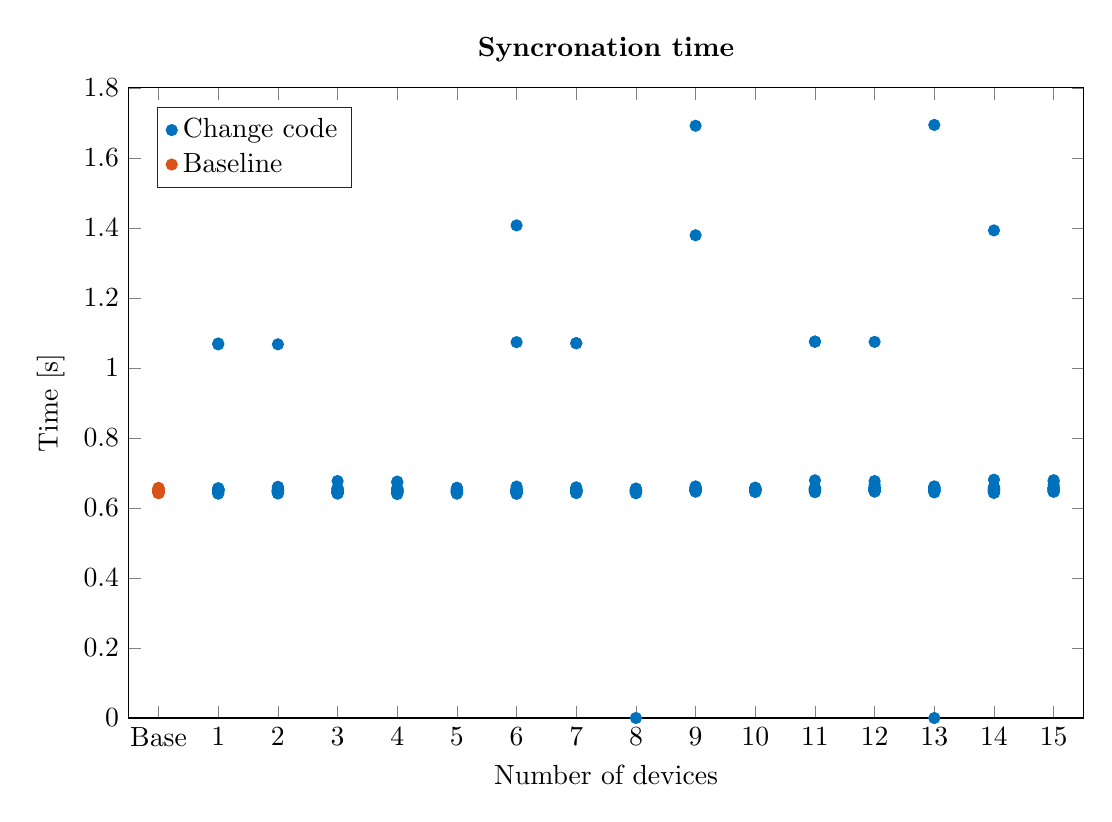
\begin{tikzpicture}

\begin{axis}[%
width=\textwidth,
height=.66\textwidth,
at={(0.758in,0.481in)},
scale only axis,
xmin=-0.5,
xmax=15.5,
xtick={0,1,2,3,4,5,6,7,8,9,10,11,12,13,14,15},
xticklabels={{Base},{1},{2},{3},{4},{5},{6},{7},{8},{9},{10},{11},{12},{13},{14},{15}},
xlabel={Number of devices},
ymin=0,
ymax=1.8,
ylabel={Time [s]},
axis background/.style={fill=white},
title style={font=\bfseries},
title={Syncronation time},
legend style={at={(0.03,0.97)},anchor=north west,legend cell align=left,align=left,draw=white!15!black}
]
\addplot [color=mycolor1,only marks,mark=*,mark options={solid}]
  table[row sep=crcr]{%
1	0.650609970092773\\
1	0.653857946395874\\
1	0.640816926956177\\
1	0.642185926437378\\
1	0.645545959472656\\
1	1.06731581687927\\
1	0.649732112884521\\
1	0.653727054595947\\
1	1.06988906860352\\
1	0.648482799530029\\
1	0.650296926498413\\
1	0.653731107711792\\
1	0.650707960128784\\
1	0.656582117080688\\
1	0.651366949081421\\
1	0.653976202011108\\
1	0.653213024139404\\
1	0.650224924087524\\
1	0.648483037948608\\
1	0.654691934585571\\
};
\addlegendentry{Change code};

\addplot [color=mycolor1,only marks,mark=*,mark options={solid},forget plot]
  table[row sep=crcr]{%
2	0.646949052810669\\
2	0.649175882339478\\
2	0.650078058242798\\
2	0.658921957015991\\
2	0.644191026687622\\
2	1.06752800941467\\
2	0.652630090713501\\
2	0.649014949798584\\
2	0.650974988937378\\
2	0.660398006439209\\
2	0.641355037689209\\
2	0.652486085891724\\
2	0.646153926849365\\
2	0.645971059799194\\
2	0.647706985473633\\
2	0.652987003326416\\
2	0.651640892028809\\
2	0.64258599281311\\
2	0.644962072372437\\
2	0.649473905563354\\
};


\addplot [color=mycolor1,only marks,mark=*,mark options={solid},forget plot]
  table[row sep=crcr]{%
3	0.643748044967651\\
3	0.644491195678711\\
3	0.642645835876465\\
3	0.656013965606689\\
3	0.647945880889893\\
3	0.646684885025024\\
3	0.641174077987671\\
3	0.647907018661499\\
3	0.644546985626221\\
3	0.645722150802612\\
3	0.64906907081604\\
3	0.648266077041626\\
3	0.642682075500488\\
3	0.652300119400024\\
3	0.641947031021118\\
3	0.676903009414673\\
3	0.648000955581665\\
3	0.655172109603882\\
3	0.648041009902954\\
3	0.656927108764648\\
};
\addplot [color=mycolor1,only marks,mark=*,mark options={solid},forget plot]
  table[row sep=crcr]{%
4	0.648493051528931\\
4	0.64559006690979\\
4	0.654642105102539\\
4	0.6754150390625\\
4	0.646654844284058\\
4	0.642754077911377\\
4	0.639609098434448\\
4	0.653938055038452\\
4	0.650071144104004\\
4	0.656721115112305\\
4	0.643237829208374\\
4	0.651222229003906\\
4	0.652673006057739\\
4	0.65081000328064\\
4	0.672778844833374\\
4	0.651262998580933\\
4	0.649074077606201\\
4	0.647204875946045\\
4	0.646042108535767\\
4	0.64453911781311\\
};
\addplot [color=mycolor1,only marks,mark=*,mark options={solid},forget plot]
  table[row sep=crcr]{%
5	0.650202989578247\\
5	0.648781776428223\\
5	0.640866994857788\\
5	0.649247169494629\\
5	0.65114688873291\\
5	0.643033027648926\\
5	0.644155025482178\\
5	0.657757997512817\\
5	0.650070905685425\\
5	0.65401291847229\\
5	0.646816968917847\\
5	0.64539098739624\\
5	0.654246091842651\\
5	0.655587911605835\\
5	0.645053863525391\\
5	0.64438796043396\\
5	0.648882150650024\\
5	0.652736902236938\\
5	0.643465995788574\\
5	0.653812170028687\\
};
\addplot [color=mycolor1,only marks,mark=*,mark options={solid},forget plot]
  table[row sep=crcr]{%
6	0.646232128143311\\
6	0.648225069046021\\
6	1.40721011161804\\
6	0.651366949081421\\
6	0.652253866195679\\
6	0.650762796401978\\
6	0.648574829101563\\
6	0.640298843383789\\
6	0.653538942337036\\
6	0.645024061203003\\
6	0.661158084869385\\
6	0.647090911865234\\
6	0.642549991607666\\
6	0.642514944076538\\
6	0.643571853637695\\
6	0.65564489364624\\
6	1.07363796234131\\
6	0.647010087966919\\
6	0.646505117416382\\
6	0.6438148021698\\
};
\addplot [color=mycolor1,only marks,mark=*,mark options={solid},forget plot]
  table[row sep=crcr]{%
7	1.07072401046753\\
7	0.652054071426392\\
7	1.07058906555176\\
7	0.648339986801147\\
7	0.652436017990112\\
7	0.642619132995605\\
7	0.643392086029053\\
7	0.648621082305908\\
7	0.645454883575439\\
7	0.652534961700439\\
7	0.64702582359314\\
7	0.644365072250366\\
7	0.659003973007202\\
7	0.652891874313354\\
7	0.646991968154907\\
7	0.655962944030762\\
7	0.651911020278931\\
7	0.649963140487671\\
7	0.650946855545044\\
7	0.650607109069824\\
};
\addplot [color=mycolor1,only marks,mark=*,mark options={solid},forget plot]
  table[row sep=crcr]{%
8	0.649052143096924\\
8	0.655632972717285\\
8	0.653681039810181\\
8	0.651021003723145\\
8	0.645121097564697\\
8	0.651643991470337\\
8	0.644710063934326\\
8	0.643614053726196\\
8	0.641947984695435\\
8	0.648487091064453\\
8	0.652446985244751\\
8	0.648170948028564\\
8	0.646777153015137\\
8	0.644640922546387\\
8	0.652256011962891\\
8	0.646914958953857\\
8	0.647845983505249\\
8	0.647209167480469\\
8	0.65062403678894\\
8	0\\
};
\addplot [color=mycolor1,only marks,mark=*,mark options={solid},forget plot]
  table[row sep=crcr]{%
9	0.650902032852173\\
9	0.653230905532837\\
9	0.651026964187622\\
9	1.37894892692566\\
9	0.658339023590088\\
9	0.6616530418396\\
9	0.650697946548462\\
9	0.65686297416687\\
9	0.646430015563965\\
9	0.652285814285278\\
9	0.657356977462769\\
9	0.648330926895142\\
9	0.652124166488647\\
9	0.650056838989258\\
9	0.649123907089233\\
9	1.69176697731018\\
9	0.648163080215454\\
9	0.653515100479126\\
9	0.648416042327881\\
9	0.652014017105103\\
};
\addplot [color=mycolor1,only marks,mark=*,mark options={solid},forget plot]
  table[row sep=crcr]{%
10	0.652431964874268\\
10	0.653368949890137\\
10	0.653976917266846\\
10	0.647805213928223\\
10	0.651004791259766\\
10	0.657984972000122\\
10	0.652050971984863\\
10	0.653388023376465\\
10	0.645644187927246\\
10	0.653051853179932\\
10	0.655381917953491\\
10	0.653103113174438\\
10	0.649111986160278\\
10	0.650975942611694\\
10	0.646430015563965\\
10	0.657355070114136\\
10	0.655450105667114\\
10	0.647177934646606\\
10	0.656944990158081\\
10	0.651263952255249\\
};
\addplot [color=mycolor1,only marks,mark=*,mark options={solid},forget plot]
  table[row sep=crcr]{%
11	0.651514053344727\\
11	0.65205192565918\\
11	0.658270835876465\\
11	0.649635076522827\\
11	1.07549595832825\\
11	0.654492855072021\\
11	0.653318881988525\\
11	0.65693998336792\\
11	0.65533185005188\\
11	1.07469415664673\\
11	0.647542953491211\\
11	0.678914070129395\\
11	0.654986143112183\\
11	0.646422863006592\\
11	0.650253057479858\\
11	0.652107954025269\\
11	0.655264139175415\\
11	0.651924133300781\\
11	0.645050048828125\\
11	0.648700952529907\\
};
\addplot [color=mycolor1,only marks,mark=*,mark options={solid},forget plot]
  table[row sep=crcr]{%
12	0.65892505645752\\
12	0.650825977325439\\
12	0.649593114852905\\
12	0.650028944015503\\
12	0.647899150848389\\
12	0.658643007278442\\
12	0.649430990219116\\
12	0.666985988616943\\
12	0.659577131271362\\
12	0.653954982757568\\
12	0.65661096572876\\
12	0.647140026092529\\
12	1.07442212104797\\
12	0.653070211410522\\
12	0.676941156387329\\
12	0.655467987060547\\
12	0.646998167037964\\
12	0.653201103210449\\
12	0.649198055267334\\
12	0.652733087539673\\
};
\addplot [color=mycolor1,only marks,mark=*,mark options={solid},forget plot]
  table[row sep=crcr]{%
13	0.647382974624634\\
13	0.653558015823364\\
13	0.647633075714111\\
13	0.650227069854736\\
13	0.655040979385376\\
13	0.644393920898438\\
13	0.656842947006226\\
13	0.650371074676514\\
13	1.69415903091431\\
13	0.651180028915405\\
13	0.649358034133911\\
13	0.650844097137451\\
13	0.659465074539185\\
13	0.648830890655518\\
13	0.65994119644165\\
13	0.655570030212402\\
13	0.661641120910645\\
13	0.654593944549561\\
13	0.656475782394409\\
13	0\\
};
\addplot [color=mycolor1,only marks,mark=*,mark options={solid},forget plot]
  table[row sep=crcr]{%
14	0.643074035644531\\
14	0.657819986343384\\
14	0.644295215606689\\
14	0.660433053970337\\
14	0.653297185897827\\
14	0.658216953277588\\
14	0.653433084487915\\
14	0.649707078933716\\
14	0.653749942779541\\
14	0.649873971939087\\
14	0.647374868392944\\
14	0.680761098861694\\
14	0.653578996658325\\
14	0.646941900253296\\
14	0.657058954238892\\
14	0.654543876647949\\
14	0.644098997116089\\
14	0.649263143539429\\
14	0.653286933898926\\
14	1.39285397529602\\
};
\addplot [color=mycolor1,only marks,mark=*,mark options={solid},forget plot]
  table[row sep=crcr]{%
15	0.654828071594238\\
15	0.648122787475586\\
15	0.656240224838257\\
15	0.646528005599976\\
15	0.648042917251587\\
15	0.657634973526001\\
15	0.656691074371338\\
15	0.654543161392212\\
15	0.665755033493042\\
15	0.655173063278198\\
15	0.675770044326782\\
15	0.679379940032959\\
15	0.654716014862061\\
15	0.655852794647217\\
15	0.657128095626831\\
15	0.646656036376953\\
15	0.647743940353394\\
15	0.651691913604736\\
15	0.657409906387329\\
15	0.656056880950928\\
};
\addplot [color=mycolor2,only marks,mark=*,mark options={solid}]
  table[row sep=crcr]
\caption{Execution time for the synchronization for different number of devices and the baseline emulator.}
\label{fig:MT_Sync_Time}
\end{figure}
\end{minipage}%
\hfill
\begin{minipage}{0.48\textwidth}
\begin{figure}[H]
\tikzsetnextfilename{MT_Sync_His}
\centering
\resizebox{\textwidth}{!}{
% This file was created by matlab2tikz.
%
%The latest updates can be retrieved from
%  http://www.mathworks.com/matlabcentral/fileexchange/22022-matlab2tikz-matlab2tikz
%where you can also make suggestions and rate matlab2tikz.
%
\definecolor{mycolor1}{rgb}{0.00000,0.44700,0.74100}%
%
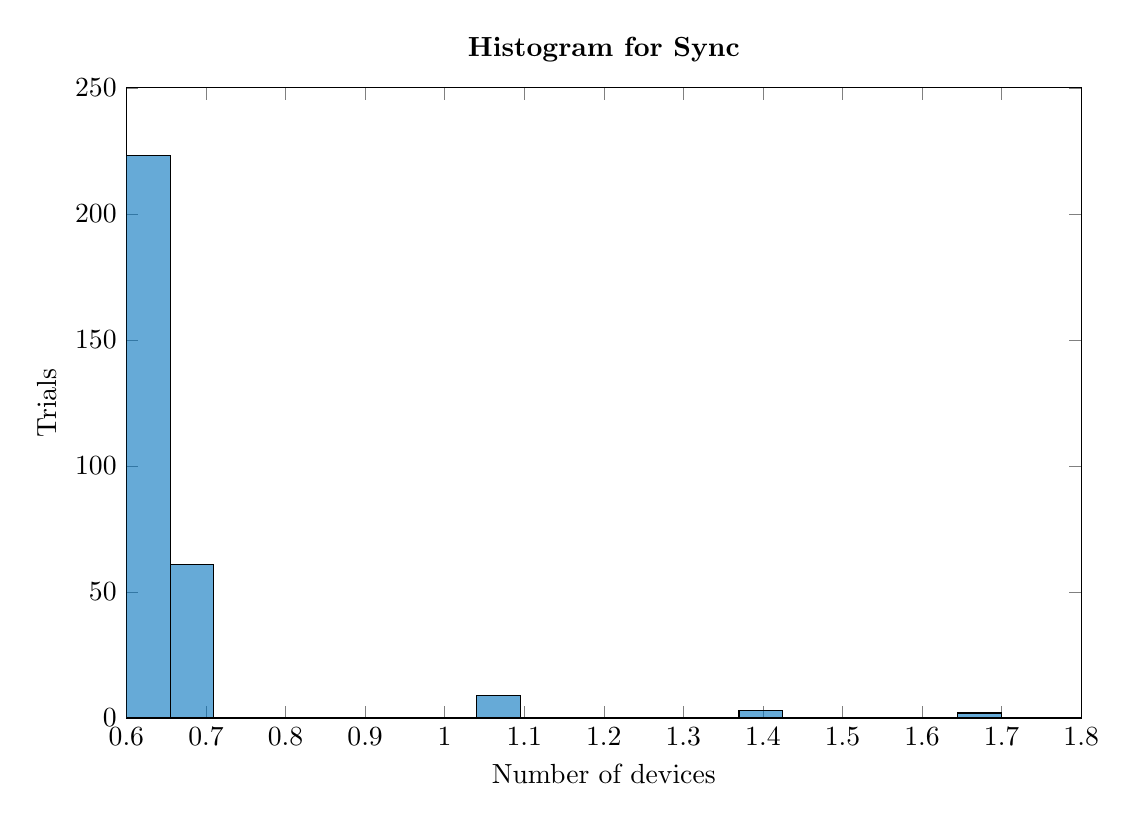
\begin{tikzpicture}

\begin{axis}[%
width=\textwidth,
height=.66\textwidth,
at={(0.758in,0.481in)},
scale only axis,
xmin=0.6,
xmax=1.8,
xlabel={Number of devices},
ymin=0,
ymax=250,
ylabel={Trials},
axis background/.style={fill=white},
title style={font=\bfseries},
title={Histogram for Sync}
]
\addplot[fill=mycolor1,fill opacity=0.6,draw=black,ybar interval,area legend] plot table[row sep=crcr] 
\caption{The distribution for the execution time for synchronization for all different number of devices.}
\label{fig:MT_Sync_His}
\end{figure}
\end{minipage}
\captionsetup{belowskip=-1.5em}

As seen on \autoref{fig:MT_Sync_Time} is the execution time for different number of devices is behaving equal to each other. Another aspect seen on the figure is that some measurements have taken some extra time to execute, but is aligning at the same time values, which also indicated on the histogram on \autoref{fig:MT_Sync_His}. Here it is seen that most measurements is placed at 0.6 s to 0.8 s and the amount at the other points is much lower. This is to be expected as the structure of the MDE only searches for the cell once independently of the number of devices.



\subsection{MIB-NB decoding}
The execution time for the MIB-NB decoding step is measured from just after a cell is found until the MIB-NB has been fully decoded, which gives the results seen on \autoref{fig:MT_MIB_Time}. However as the MDE sometimes fails, which results in it retrying the decoding, a bias is made to only use the time for the final and successful decoding of MIB-NB.


\captionsetup{belowskip=0em}
\begin{minipage}{0.48\textwidth}
\begin{figure}[H]
\tikzsetnextfilename{MT_MIB_Time}
\centering
\resizebox{\textwidth}{!}{
% This file was created by matlab2tikz.
%
%The latest updates can be retrieved from
%  http://www.mathworks.com/matlabcentral/fileexchange/22022-matlab2tikz-matlab2tikz
%where you can also make suggestions and rate matlab2tikz.
%
\definecolor{mycolor1}{rgb}{0.00000,0.44700,0.74100}%
\definecolor{mycolor2}{rgb}{0.85000,0.32500,0.09800}%
%
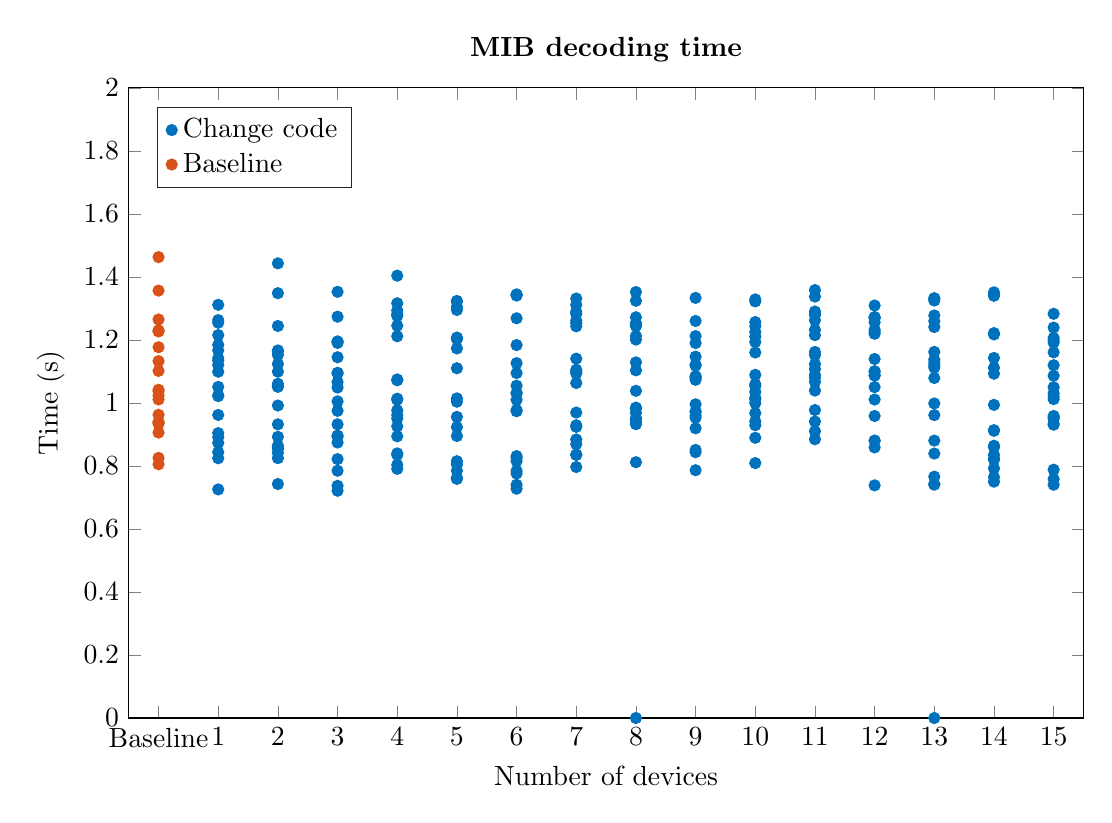
\begin{tikzpicture}

\begin{axis}[%
width=\textwidth,
height=.66\textwidth,
at={(0.758in,0.481in)},
scale only axis,
xmin=-0.5,
xmax=15.5,
xtick={0,1,2,3,4,5,6,7,8,9,10,11,12,13,14,15},
xticklabels={{Baseline},{1},{2},{3},{4},{5},{6},{7},{8},{9},{10},{11},{12},{13},{14},{15}},
xlabel={Number of devices},
ymin=0,
ymax=2,
ylabel={Time (s)},
axis background/.style={fill=white},
title style={font=\bfseries},
title={MIB decoding time},
legend style={at={(0.03,0.97)},anchor=north west,legend cell align=left,align=left,draw=white!15!black}
]
\addplot [color=mycolor1,only marks,mark=*,mark options={solid}]
  table[row sep=crcr]{%
1	1.18452787399292\\
1	1.02464199066162\\
1	1.16689705848694\\
1	0.904258966445923\\
1	0.843533992767334\\
1	1.13420486450195\\
1	0.824519872665405\\
1	0.961822032928467\\
1	0.891458988189697\\
1	1.3114321231842\\
1	0.72556209564209\\
1	1.26286196708679\\
1	1.25451898574829\\
1	1.12048602104187\\
1	1.02167701721191\\
1	1.09917998313904\\
1	0.873126983642578\\
1	1.14201807975769\\
1	1.21537899971008\\
1	1.05097317695618\\
};
\addlegendentry{Change code};

\addplot [color=mycolor1,only marks,mark=*,mark options={solid},forget plot]
  table[row sep=crcr]{%
2	0.742633819580078\\
2	1.12349700927734\\
2	0.862571001052856\\
2	1.09928011894226\\
2	1.06075310707092\\
2	0.841415166854858\\
2	0.824921131134033\\
2	1.05261611938477\\
2	1.0511691570282\\
2	1.34838080406189\\
2	1.16666889190674\\
2	0.892491817474365\\
2	0.863969087600708\\
2	0.991780996322632\\
2	1.16264510154724\\
2	1.15249800682068\\
2	1.24425196647644\\
2	0.853885173797607\\
2	1.44308090209961\\
2	0.932136058807373\\
};


\addplot [color=mycolor1,only marks,mark=*,mark options={solid},forget plot]
  table[row sep=crcr]{%
3	1.35272288322449\\
3	0.896404027938843\\
3	1.19529414176941\\
3	0.721312999725342\\
3	1.00501799583435\\
3	0.974997997283936\\
3	1.27371096611023\\
3	1.09565401077271\\
3	1.19446611404419\\
3	0.736949920654297\\
3	0.784852981567383\\
3	0.874388933181763\\
3	0.932243824005127\\
3	0.821744918823242\\
3	1.09404897689819\\
3	1.14502000808716\\
3	0.893469095230103\\
3	1.19056606292725\\
3	1.06648683547974\\
3	1.04886889457703\\
};
\addplot [color=mycolor1,only marks,mark=*,mark options={solid},forget plot]
  table[row sep=crcr]{%
4	1.21173596382141\\
4	0.894090890884399\\
4	0.950580835342407\\
4	1.31642508506775\\
4	0.83543586730957\\
4	0.925927877426147\\
4	0.976491928100586\\
4	1.28235483169556\\
4	0.803546905517578\\
4	0.790771007537842\\
4	1.27620601654053\\
4	1.01348495483398\\
4	1.07200884819031\\
4	1.01012992858887\\
4	0.839915037155151\\
4	0.962180137634277\\
4	1.07453393936157\\
4	1.29357409477234\\
4	1.40396094322205\\
4	1.24524092674255\\
};
\addplot [color=mycolor1,only marks,mark=*,mark options={solid},forget plot]
  table[row sep=crcr]{%
5	1.29511213302612\\
5	1.01446914672852\\
5	1.20752096176147\\
5	1.20313382148743\\
5	0.805004119873047\\
5	1.30468487739563\\
5	0.815110921859741\\
5	0.758973121643066\\
5	1.11016798019409\\
5	0.761851072311401\\
5	0.955629825592041\\
5	1.00391411781311\\
5	1.32148098945618\\
5	1.17293000221252\\
5	0.923401832580566\\
5	0.895086050033569\\
5	1.20391082763672\\
5	0.76114296913147\\
5	0.784970045089722\\
5	1.32375192642212\\
};
\addplot [color=mycolor1,only marks,mark=*,mark options={solid},forget plot]
  table[row sep=crcr]{%
6	1.12626886367798\\
6	0.784417867660522\\
6	0.973766088485718\\
6	1.34400105476379\\
6	1.03182911872864\\
6	1.00979208946228\\
6	1.18366503715515\\
6	0.977426052093506\\
6	0.831204891204834\\
6	1.34424090385437\\
6	1.26865386962891\\
6	0.815386056900024\\
6	0.72773003578186\\
6	1.09482884407043\\
6	0.776089191436768\\
6	1.34079313278198\\
6	0.740194082260132\\
6	0.825405120849609\\
6	1.03018093109131\\
6	1.05475306510925\\
};
\addplot [color=mycolor1,only marks,mark=*,mark options={solid},forget plot]
  table[row sep=crcr]{%
7	1.14058113098145\\
7	0.969480037689209\\
7	1.2895450592041\\
7	1.25373196601868\\
7	0.869355916976929\\
7	0.836460828781128\\
7	0.883985042572021\\
7	1.33135199546814\\
7	1.10523915290833\\
7	1.06331515312195\\
7	0.834944009780884\\
7	0.796628952026367\\
7	1.09889316558838\\
7	1.26145696640015\\
7	1.31127190589905\\
7	0.929186105728149\\
7	1.09361791610718\\
7	0.924177885055542\\
7	1.28277397155762\\
7	1.24324703216553\\
};
\addplot [color=mycolor1,only marks,mark=*,mark options={solid},forget plot]
  table[row sep=crcr]{%
8	1.21215677261353\\
8	0.811891078948975\\
8	1.35208201408386\\
8	1.25351810455322\\
8	1.24444103240967\\
8	0.96881103515625\\
8	1.32427191734314\\
8	1.24557089805603\\
8	0.985246181488037\\
8	1.10344481468201\\
8	0.947085857391357\\
8	1.03846478462219\\
8	0.940639019012451\\
8	1.27187204360962\\
8	0.932521820068359\\
8	1.20112204551697\\
8	0.952279090881348\\
8	0.981828927993774\\
8	1.12882900238037\\
8	0\\
};
\addplot [color=mycolor1,only marks,mark=*,mark options={solid},forget plot]
  table[row sep=crcr]{%
9	1.07991504669189\\
9	1.19017219543457\\
9	1.26013112068176\\
9	1.21215891838074\\
9	0.786477088928223\\
9	1.14683389663696\\
9	0.953114032745361\\
9	0.919471025466919\\
9	1.3333580493927\\
9	1.07340693473816\\
9	0.95987606048584\\
9	0.84372091293335\\
9	0.995597839355469\\
9	1.08392119407654\\
9	0.971073150634766\\
9	1.1183009147644\\
9	1.08447599411011\\
9	0.850917100906372\\
9	0.973115921020508\\
9	1.12152695655823\\
};
\addplot [color=mycolor1,only marks,mark=*,mark options={solid},forget plot]
  table[row sep=crcr]{%
10	1.25671696662903\\
10	1.05311989784241\\
10	0.929455041885376\\
10	1.19342279434204\\
10	1.05944609642029\\
10	1.01689720153809\\
10	0.967733860015869\\
10	1.21085119247437\\
10	1.22501087188721\\
10	1.08909916877747\\
10	0.941591024398804\\
10	1.1600980758667\\
10	1.24331402778625\\
10	0.889430046081543\\
10	1.32221412658691\\
10	1.01067590713501\\
10	0.999495983123779\\
10	1.3286120891571\\
10	1.03497505187988\\
10	0.809139966964722\\
};
\addplot [color=mycolor1,only marks,mark=*,mark options={solid},forget plot]
  table[row sep=crcr]{%
11	0.941027879714966\\
11	1.35822701454163\\
11	0.977467060089111\\
11	1.29018783569336\\
11	1.10762286186218\\
11	1.12313294410706\\
11	1.08049416542053\\
11	1.08900213241577\\
11	1.15175604820251\\
11	1.06713485717773\\
11	1.1618390083313\\
11	1.21526479721069\\
11	1.33760190010071\\
11	0.884803056716919\\
11	1.23175096511841\\
11	0.910167932510376\\
11	1.27922487258911\\
11	1.03915095329285\\
11	1.28432893753052\\
11	1.26249885559082\\
};
\addplot [color=mycolor1,only marks,mark=*,mark options={solid},forget plot]
  table[row sep=crcr]{%
12	0.858820915222168\\
12	1.21957588195801\\
12	0.880445003509521\\
12	1.05029010772705\\
12	1.23261284828186\\
12	1.30926299095154\\
12	0.879901170730591\\
12	1.27121210098267\\
12	1.13944888114929\\
12	0.958610057830811\\
12	1.08663201332092\\
12	1.01077389717102\\
12	1.08854699134827\\
12	1.2690908908844\\
12	1.22531986236572\\
12	1.09908199310303\\
12	1.27269697189331\\
12	1.25594997406006\\
12	1.10074591636658\\
12	0.738483905792236\\
};
\addplot [color=mycolor1,only marks,mark=*,mark options={solid},forget plot]
  table[row sep=crcr]{%
13	0.83938193321228\\
13	0.998347997665405\\
13	1.32503414154053\\
13	0.880541086196899\\
13	1.16189002990723\\
13	0.742758989334106\\
13	0.765993118286133\\
13	1.25955986976624\\
13	1.0792031288147\\
13	0.740605115890503\\
13	1.33235692977905\\
13	1.11989402770996\\
13	1.13771796226501\\
13	1.11200213432312\\
13	1.1292519569397\\
13	0.961405992507935\\
13	1.27758502960205\\
13	1.24095487594604\\
13	1.33164381980896\\
13	0\\
};
\addplot [color=mycolor1,only marks,mark=*,mark options={solid},forget plot]
  table[row sep=crcr]{%
14	0.835340976715088\\
14	1.21743702888489\\
14	1.1116509437561\\
14	0.764328956604004\\
14	1.3510730266571\\
14	1.34011006355286\\
14	0.861910104751587\\
14	1.09282898902893\\
14	1.14283895492554\\
14	1.34170484542847\\
14	0.792457103729248\\
14	0.864109992980957\\
14	0.750169038772583\\
14	1.22165703773499\\
14	0.819968938827515\\
14	0.823435068130493\\
14	0.993892908096313\\
14	0.913672924041748\\
14	0.91166090965271\\
14	0.859905958175659\\
};
\addplot [color=mycolor1,only marks,mark=*,mark options={solid},forget plot]
  table[row sep=crcr]{%
15	0.958617925643921\\
15	1.01214718818665\\
15	1.23916387557983\\
15	0.954987049102783\\
15	1.02038717269897\\
15	0.949368000030518\\
15	1.08639097213745\\
15	1.20632886886597\\
15	1.28288388252258\\
15	1.04977297782898\\
15	0.788140058517456\\
15	0.933758020401001\\
15	1.16064596176147\\
15	0.740518093109131\\
15	1.11970591545105\\
15	1.19137382507324\\
15	0.931004047393799\\
15	0.758590936660767\\
15	1.19861912727356\\
15	1.03083515167236\\
};
\addplot [color=mycolor2,only marks,mark=*,mark options={solid}]
  table[row sep=crcr]
\caption{Execution time for the decoding the MIB-NB for different number of devices and the baseline emulator. A single measurement for the base line is placed at 5.0834 s, which is not shown on this figure.}
\label{fig:MT_MIB_Time}
\end{figure}
\end{minipage}%
\hfill
\begin{minipage}{0.48\textwidth}
\begin{figure}[H]
\tikzsetnextfilename{MT_MIB_His}
\centering
\resizebox{\textwidth}{!}{
% This file was created by matlab2tikz.
%
%The latest updates can be retrieved from
%  http://www.mathworks.com/matlabcentral/fileexchange/22022-matlab2tikz-matlab2tikz
%where you can also make suggestions and rate matlab2tikz.
%
\definecolor{mycolor1}{rgb}{0.00000,0.44700,0.74100}%
%
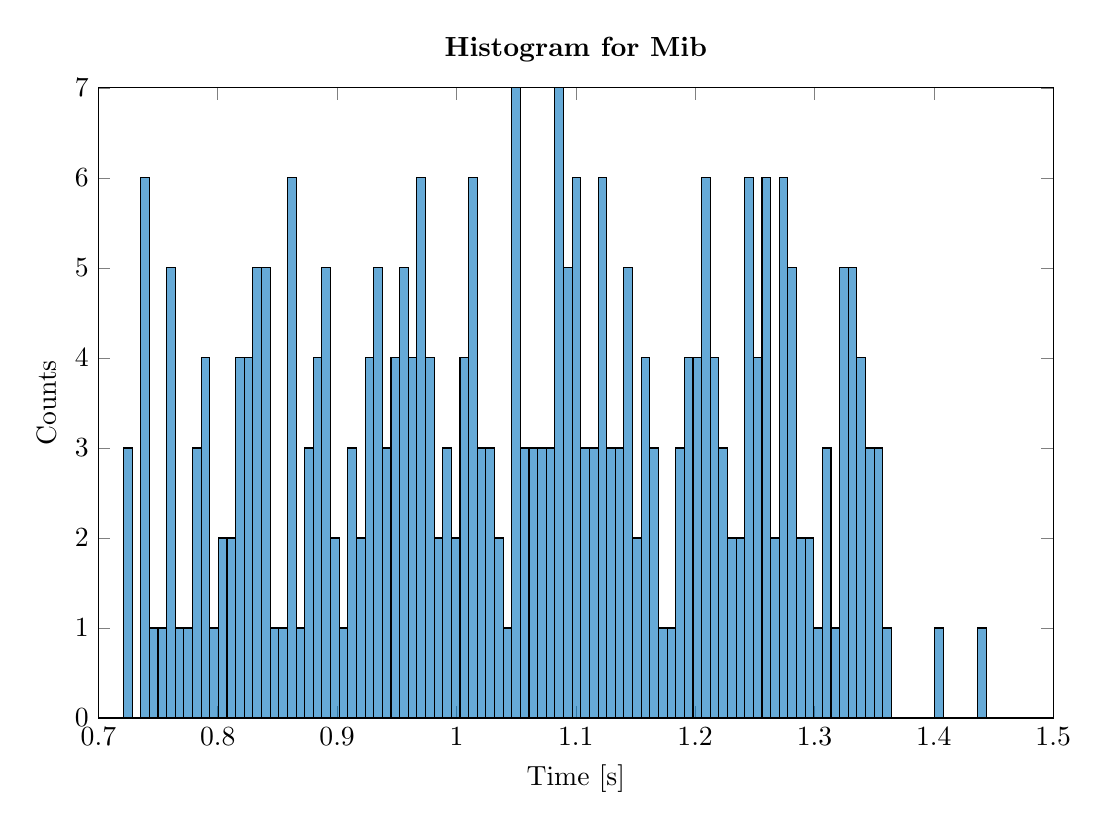
\begin{tikzpicture}

\begin{axis}[%
width=\textwidth,
height=.66\textwidth,
at={(0.758in,0.481in)},
scale only axis,
xmin=0.7,
xmax=1.5,
xlabel={Time [s]},
ymin=0,
ymax=7,
ylabel={Counts},
axis background/.style={fill=white},
title style={font=\bfseries},
title={Histogram for Mib}
]
\addplot[fill=mycolor1,fill opacity=0.6,draw=black,ybar interval,area legend] plot table[row sep=crcr] {%
x	y\\
0.721	3\\
0.72823	0\\
0.73546	6\\
0.74269	1\\
0.74992	1\\
0.75715	5\\
0.76438	1\\
0.77161	1\\
0.77884	3\\
0.78607	4\\
0.7933	1\\
0.80053	2\\
0.80776	2\\
0.81499	4\\
0.82222	4\\
0.82945	5\\
0.83668	5\\
0.84391	1\\
0.85114	1\\
0.85837	6\\
0.8656	1\\
0.87283	3\\
0.88006	4\\
0.88729	5\\
0.89452	2\\
0.90175	1\\
0.90898	3\\
0.91621	2\\
0.92344	4\\
0.93067	5\\
0.9379	3\\
0.94513	4\\
0.95236	5\\
0.95959	4\\
0.96682	6\\
0.97405	4\\
0.98128	2\\
0.98851	3\\
0.99574	2\\
1.00297	4\\
1.0102	6\\
1.01743	3\\
1.02466	3\\
1.03189	2\\
1.03912	1\\
1.04635	7\\
1.05358	3\\
1.06081	3\\
1.06804	3\\
1.07527	3\\
1.0825	7\\
1.08973	5\\
1.09696	6\\
1.10419	3\\
1.11142	3\\
1.11865	6\\
1.12588	3\\
1.13311	3\\
1.14034	5\\
1.14757	2\\
1.1548	4\\
1.16203	3\\
1.16926	1\\
1.17649	1\\
1.18372	3\\
1.19095	4\\
1.19818	4\\
1.20541	6\\
1.21264	4\\
1.21987	3\\
1.2271	2\\
1.23433	2\\
1.24156	6\\
1.24879	4\\
1.25602	6\\
1.26325	2\\
1.27048	6\\
1.27771	5\\
1.28494	2\\
1.29217	2\\
1.2994	1\\
1.30663	3\\
1.31386	1\\
1.32109	5\\
1.32832	5\\
1.33555	4\\
1.34278	3\\
1.35001	3\\
1.35724	1\\
1.36447	0\\
1.3717	0\\
1.37893	0\\
1.38616	0\\
1.39339	0\\
1.40062	1\\
1.40785	0\\
1.41508	0\\
1.42231	0\\
1.42954	0\\
1.43677	1\\
1.444	1\\
};
\end{axis}
\end{tikzpicture}%}
\caption{The distribution for the execution time for decoding the MIB-NB for all different number of devices.}
\label{fig:MT_MIB_His}
\end{figure}
\end{minipage}
\captionsetup{belowskip=-1.5em}

As seen on \autoref{fig:MT_MIB_Time} the execution time for the MIB-NB decoding quite stable independently on the number of devices. The spread is big compared to the synchronazitation step, which also can be seen when comparing the histogram for the two steps, \autoref{fig:MT_Sync_His} and \autoref{fig:MT_MIB_His}. The baseline emulator have the same tendency as the MDE, which indicates that the changes do not effect this step, as expected. On \autoref{fig:MT_MIB_Tries} is it shown how many attempts the different measurements needed before completing the MIB-NB decoding step.

\begin{figure}[H]
\tikzsetnextfilename{MT_MIB_Tries}
\centering
%\resizebox{0.5\textwidth}{!}{
% This file was created by matlab2tikz.
%
%The latest updates can be retrieved from
%  http://www.mathworks.com/matlabcentral/fileexchange/22022-matlab2tikz-matlab2tikz
%where you can also make suggestions and rate matlab2tikz.
%
\definecolor{mycolor1}{rgb}{0.20810,0.16630,0.52920}%
\definecolor{mycolor2}{rgb}{0.02650,0.61370,0.81350}%
\definecolor{mycolor3}{rgb}{0.64730,0.74560,0.41880}%
\definecolor{mycolor4}{rgb}{0.97630,0.98310,0.05380}%
%
\begin{tikzpicture}

\begin{axis}[%
width=\textwidth,
height=.66\textwidth,
at={(0.607in,0.481in)},
scale only axis,
bar width=0.5,
xmin=-0.5,
xmax=15.5,
xtick={0,1,2,3,4,5,6,7,8,9,10,11,12,13,14,15},
xticklabels={{Baseline},{1},{2},{3},{4},{5},{6},{7},{8},{9},{10},{11},{12},{13},{14},{15}},
xlabel={Number of devices},
ymin=0,
ymax=1,
ylabel={Trials},
axis background/.style={fill=white},
title style={font=\bfseries},
title={Number of tries for decoding MIB},
legend style={at={(1.03,1)},anchor=north west,legend cell align=left,align=left,draw=white!15!black}
]
\addplot[ybar stacked,draw=black,fill=mycolor1,area legend] plot table[row sep=crcr] {%
0	0.65\\
1	0.8\\
2	0.85\\
3	0.75\\
4	0.9\\
5	0.65\\
6	0.85\\
7	0.85\\
8	0.736842105263158\\
9	0.9\\
10	0.95\\
11	0.95\\
12	1\\
13	0.842105263157895\\
14	0.95\\
15	0.95\\
};
\addlegendentry{1 Attempts};

\addplot[ybar stacked,draw=black,fill=mycolor2,area legend] plot table[row sep=crcr] {%
0	0.25\\
1	0.15\\
2	0.05\\
3	0.2\\
4	0.1\\
5	0.25\\
6	0\\
7	0.15\\
8	0.263157894736842\\
9	0.1\\
10	0.05\\
11	0.05\\
12	0\\
13	0.157894736842105\\
14	0.05\\
15	0.05\\
};
\addlegendentry{2 Attempts};

\addplot[ybar stacked,draw=black,fill=mycolor3,area legend] plot table[row sep=crcr] {%
0	0.1\\
1	0.05\\
2	0.05\\
3	0.05\\
4	0\\
5	0.05\\
6	0.15\\
7	0\\
8	0\\
9	0\\
10	0\\
11	0\\
12	0\\
13	0\\
14	0\\
15	0\\
};
\addlegendentry{3 Attempts};

\addplot[ybar stacked,draw=black,fill=mycolor4,area legend] plot table[row sep=crcr] {%
0	0\\
1	0\\
2	0.05\\
3	0\\
4	0\\
5	0.05\\
6	0\\
7	0\\
8	0\\
9	0\\
10	0\\
11	0\\
12	0\\
13	0\\
14	0\\
15	0\\
};
\addlegendentry{4 Attempts};

\end{axis}
\end{tikzpicture}%
\caption{The distribution for number of attempts for decoding the MIB-NB for different number of devices.}
\label{fig:MT_MIB_Tries}
\end{figure}

It is seen on \autoref{fig:MT_MIB_Tries} that baseline emulator is not different from the MDE at a lower number of devices. At a higher number of devices it even seems like the MDE is more efficient, as the failed attempts decreases when the number of devices increases.

\subsection{NB-SIB1}
The execution time for the NB-SIB1 decoding step is measured from the MIB-NB is decoded to the NB-SIB1 is fully decoded, which gives the results seen on \autoref{fig:MT_SIB1_Time}. The test is executed with the different number of devices, but the results shown on \autoref{fig:MT_SIB1_Time} is only for one of the emulated devices, as each device demodulates the NB-SIB1 individually. This is done, so all number of devices have the same stand point compared to the measurements.
As both the radio error and idle after MIB-NB error occurs in this step of the process, the number of measurement points are lowered further.

\captionsetup{belowskip=0em}
\begin{minipage}{0.48\textwidth}
\begin{figure}[H]
\tikzsetnextfilename{MT_SIB1_Time}
\centering
\resizebox{\textwidth}{!}{
% This file was created by matlab2tikz.
%
%The latest updates can be retrieved from
%  http://www.mathworks.com/matlabcentral/fileexchange/22022-matlab2tikz-matlab2tikz
%where you can also make suggestions and rate matlab2tikz.
%
\definecolor{mycolor1}{rgb}{0.00000,0.44700,0.74100}%
\definecolor{mycolor2}{rgb}{0.85000,0.32500,0.09800}%
%
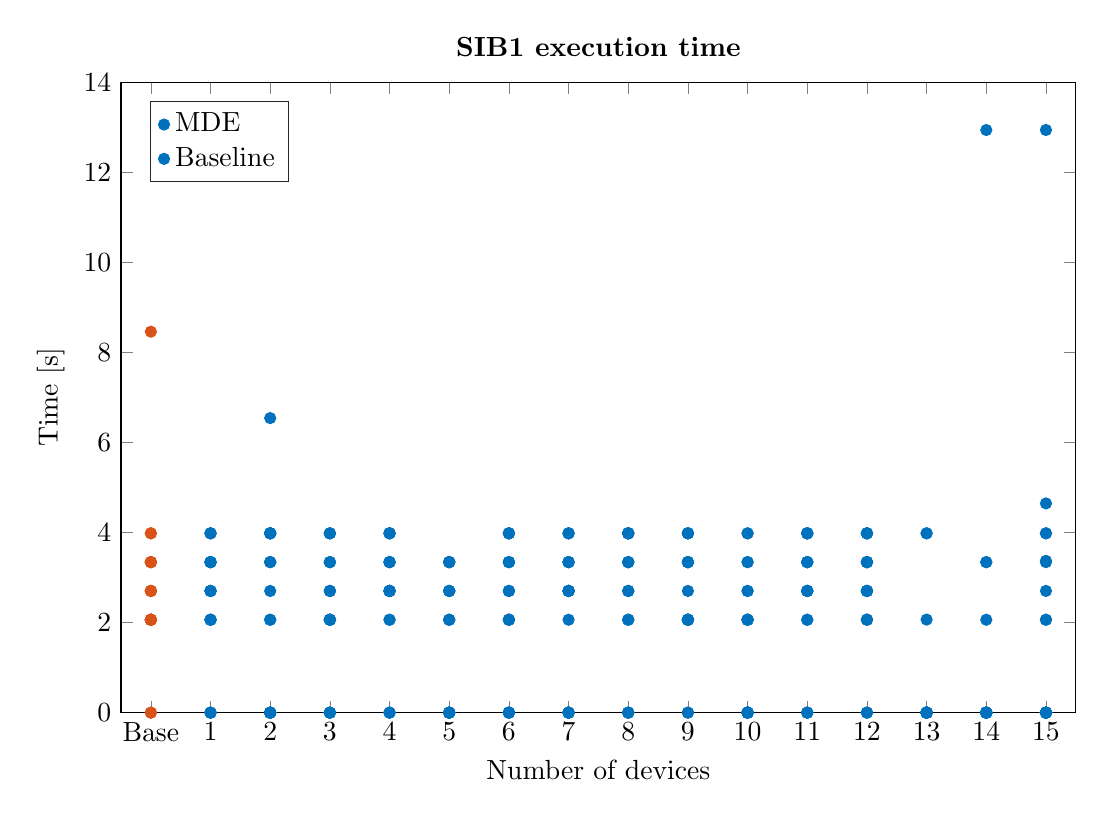
\begin{tikzpicture}

\begin{axis}[%
width=\textwidth,
height=.66\textwidth,
at={(0.758in,0.481in)},
scale only axis,
xmin=-0.5,
xmax=15.5,
xtick={0,1,2,3,4,5,6,7,8,9,10,11,12,13,14,15},
xticklabels={{Base},{1},{2},{3},{4},{5},{6},{7},{8},{9},{10},{11},{12},{13},{14},{15}},
xlabel={Number of devices},
ymin=0,
ymax=14,
ylabel={Time [s]},
axis background/.style={fill=white},
title style={font=\bfseries},
title={SIB1 execution time},
legend style={at={(0.03,0.97)},anchor=north west,legend cell align=left,align=left,draw=white!15!black}
]
\addplot [color=mycolor1,only marks,mark=*,mark options={solid}]
  table[row sep=crcr]{%
1	2.06326198577881\\
1	2.06440305709839\\
1	3.98324704170227\\
1	3.34370994567871\\
1	2.064288854599\\
1	2.06284713745117\\
1	3.34417414665222\\
1	0\\
1	3.98412108421326\\
1	0\\
1	0\\
1	3.34290599822998\\
1	3.98381996154785\\
1	2.70346093177795\\
1	2.7038140296936\\
1	3.34348487854004\\
1	2.70364594459534\\
1	3.34404802322388\\
1	2.70409893989563\\
1	0\\
};
\addlegendentry{MDE};

\addplot [color=mycolor1,only marks,mark=*,mark options={solid},forget plot]
  table[row sep=crcr]{%
2	0\\
2	2.06386804580688\\
2	3.9830470085144\\
2	2.70327496528625\\
2	3.98435401916504\\
2	3.34425902366638\\
2	0\\
2	0\\
2	3.34448194503784\\
2	3.98420310020447\\
2	3.98417806625366\\
2	0\\
2	0\\
2	0\\
2	2.06371593475342\\
2	0\\
2	3.98412013053894\\
2	6.54380798339844\\
2	3.34428119659424\\
2	0\\
};

\addplot [color=mycolor1,only marks,mark=*,mark options={solid}]
  table[row sep=crcr]{%
3	0\\
3	3.34311699867249\\
3	2.06403684616089\\
3	2.06435298919678\\
3	2.06442618370056\\
3	3.98329901695251\\
3	0\\
3	2.06374597549438\\
3	3.98314690589905\\
3	2.70358204841614\\
3	3.34318780899048\\
3	3.98370504379272\\
3	0\\
3	2.70299601554871\\
3	0\\
3	0\\
3	3.34412288665771\\
3	2.70408582687378\\
3	2.06382894515991\\
3	2.06484198570251\\
};
\addplot [color=mycolor1,only marks,mark=*,mark options={solid},forget plot]
  table[row sep=crcr]{%
4	3.34450602531433\\
4	2.70465612411499\\
4	3.9842541217804\\
4	0\\
4	0\\
4	2.70361804962158\\
4	3.34443497657776\\
4	3.3442051410675\\
4	3.98412203788757\\
4	0\\
4	2.70440602302551\\
4	2.70354795455933\\
4	3.98445606231689\\
4	3.34337210655212\\
4	2.7031729221344\\
4	2.06350088119507\\
4	2.7041220664978\\
4	3.98393082618713\\
4	2.7035870552063\\
4	2.06354808807373\\
};
\addplot [color=mycolor1,only marks,mark=*,mark options={solid},forget plot]
  table[row sep=crcr]{%
5	2.70302295684814\\
5	2.0638120174408\\
5	2.70368385314941\\
5	3.34371113777161\\
5	3.34336185455322\\
5	0\\
5	0\\
5	2.06377196311951\\
5	3.34426617622375\\
5	0\\
5	0\\
5	2.06288194656372\\
5	2.70433521270752\\
5	2.70352816581726\\
5	0\\
5	0\\
5	0\\
5	0\\
5	3.34436511993408\\
5	3.34376907348633\\
};
\addplot [color=mycolor1,only marks,mark=*,mark options={solid},forget plot]
  table[row sep=crcr]{%
6	2.70398306846619\\
6	3.98413896560669\\
6	2.70379996299744\\
6	2.06457901000977\\
6	3.34415984153748\\
6	2.06386399269104\\
6	0\\
6	3.98335313796997\\
6	2.06371712684631\\
6	3.34421420097351\\
6	3.98331713676453\\
6	0\\
6	3.98413610458374\\
6	2.06382918357849\\
6	0\\
6	3.34377503395081\\
6	0\\
6	0\\
6	3.34429097175598\\
6	2.70383501052856\\
};
\addplot [color=mycolor1,only marks,mark=*,mark options={solid},forget plot]
  table[row sep=crcr]{%
7	2.70354390144348\\
7	0\\
7	2.70460295677185\\
7	3.34423208236694\\
7	0\\
7	2.70423698425293\\
7	2.06377696990967\\
7	0\\
7	0\\
7	0\\
7	3.98403000831604\\
7	3.34456205368042\\
7	3.98315095901489\\
7	3.34323811531067\\
7	2.70326495170593\\
7	3.34363293647766\\
7	0\\
7	2.70313405990601\\
7	3.98417210578918\\
7	2.70344686508179\\
};
\addplot [color=mycolor1,only marks,mark=*,mark options={solid},forget plot]
  table[row sep=crcr]{%
8	3.34394001960754\\
8	3.9837920665741\\
8	3.98305892944336\\
8	2.06428194046021\\
8	0\\
8	2.06423997879028\\
8	3.9834680557251\\
8	0\\
8	2.70423197746277\\
8	3.34431982040405\\
8	0\\
8	2.7035391330719\\
8	0\\
8	3.34361791610718\\
8	2.06392502784729\\
8	3.98410606384277\\
8	2.70362114906311\\
8	3.34315776824951\\
8	3.98356890678406\\
8	3.98443794250488\\
};
\addplot [color=mycolor1,only marks,mark=*,mark options={solid},forget plot]
  table[row sep=crcr]{%
9	2.06394577026367\\
9	3.34412384033203\\
9	3.98399186134338\\
9	3.9841251373291\\
9	2.06348896026611\\
9	0\\
9	3.34316611289978\\
9	2.06286597251892\\
9	3.98410415649414\\
9	2.06404900550842\\
9	2.06381487846375\\
9	2.06389117240906\\
9	0\\
9	2.06410598754883\\
9	2.70342183113098\\
9	3.34323501586914\\
9	3.34321093559265\\
9	3.98393988609314\\
9	2.06367611885071\\
9	3.34430599212646\\
};
\addplot [color=mycolor1,only marks,mark=*,mark options={solid},forget plot]
  table[row sep=crcr]{%
10	0\\
10	3.98293900489807\\
10	3.34414911270142\\
10	2.06450819969177\\
10	0\\
10	0\\
10	0\\
10	3.34374499320984\\
10	0\\
10	0\\
10	3.98308205604553\\
10	2.06371092796326\\
10	2.06403684616089\\
10	2.06367516517639\\
10	0\\
10	2.7036759853363\\
10	2.06395602226257\\
10	2.70334911346436\\
10	0\\
10	0\\
};
\addplot [color=mycolor1,only marks,mark=*,mark options={solid},forget plot]
  table[row sep=crcr]{%
11	3.34377312660217\\
11	2.70394802093506\\
11	2.7042019367218\\
11	3.98395895957947\\
11	0\\
11	3.34369802474976\\
11	2.70436382293701\\
11	2.70322489738464\\
11	3.34422206878662\\
11	2.70361518859863\\
11	3.98409199714661\\
11	3.34430408477783\\
11	0\\
11	3.98311901092529\\
11	3.98332715034485\\
11	2.06374907493591\\
11	0\\
11	0\\
11	3.98366022109985\\
11	2.06314301490784\\
};
\addplot [color=mycolor1,only marks,mark=*,mark options={solid},forget plot]
  table[row sep=crcr]{%
12	2.7039110660553\\
12	2.06496000289917\\
12	2.70287799835205\\
12	2.7045431137085\\
12	3.98310804367065\\
12	2.70452785491943\\
12	3.34418082237244\\
12	0\\
12	3.98356199264526\\
12	0\\
12	3.34408807754517\\
12	3.34393095970154\\
12	3.98390102386475\\
12	0\\
12	3.98423719406128\\
12	3.34313797950745\\
12	2.70388698577881\\
12	3.34319090843201\\
12	2.06460905075073\\
12	2.06348609924316\\
};
\addplot [color=mycolor1,only marks,mark=*,mark options={solid},forget plot]
  table[row sep=crcr]{%
13	0\\
13	0\\
13	0\\
13	0\\
13	3.98369693756104\\
13	0\\
13	0\\
13	0\\
13	0\\
13	0\\
13	0\\
13	0\\
13	0\\
13	0\\
13	3.98429584503174\\
13	0\\
13	0\\
13	0\\
13	0\\
13	2.06700801849365\\
};
\addplot [color=mycolor1,only marks,mark=*,mark options={solid},forget plot]
  table[row sep=crcr]{%
14	0\\
14	2.06355404853821\\
14	0\\
14	0\\
14	0\\
14	0\\
14	0\\
14	3.34336185455322\\
14	0\\
14	0\\
14	3.34429407119751\\
14	0\\
14	0\\
14	0\\
14	0\\
14	0\\
14	12.9436860084534\\
14	0\\
14	0\\
14	0\\
};
\addplot [color=mycolor1,only marks,mark=*,mark options={solid},forget plot]
  table[row sep=crcr]{%
15	3.37162494659424\\
15	0\\
15	2.06366395950317\\
15	2.70392298698425\\
15	0\\
15	3.98395490646362\\
15	0\\
15	12.9445569515228\\
15	0\\
15	0\\
15	0\\
15	0\\
15	3.34374690055847\\
15	0\\
15	3.98381996154785\\
15	4.64827418327332\\
15	0\\
15	2.06406998634338\\
15	0\\
15	0\\
};
\addplot [color=mycolor2,only marks,mark=*,mark options={solid}]
  table[row sep=crcr]
\caption{Execution time for the decoding the NB-SIB1 step for different number of devices and the baseline emulator.}
\label{fig:MT_SIB1_Time}
\end{figure}
\end{minipage}%
\hfill
\begin{minipage}{0.48\textwidth}
\begin{figure}[H]
\tikzsetnextfilename{MT_SIB1_His}
\centering
\resizebox{\textwidth}{!}{
% This file was created by matlab2tikz.
%
%The latest updates can be retrieved from
%  http://www.mathworks.com/matlabcentral/fileexchange/22022-matlab2tikz-matlab2tikz
%where you can also make suggestions and rate matlab2tikz.
%
\definecolor{mycolor1}{rgb}{0.00000,0.44700,0.74100}%
%
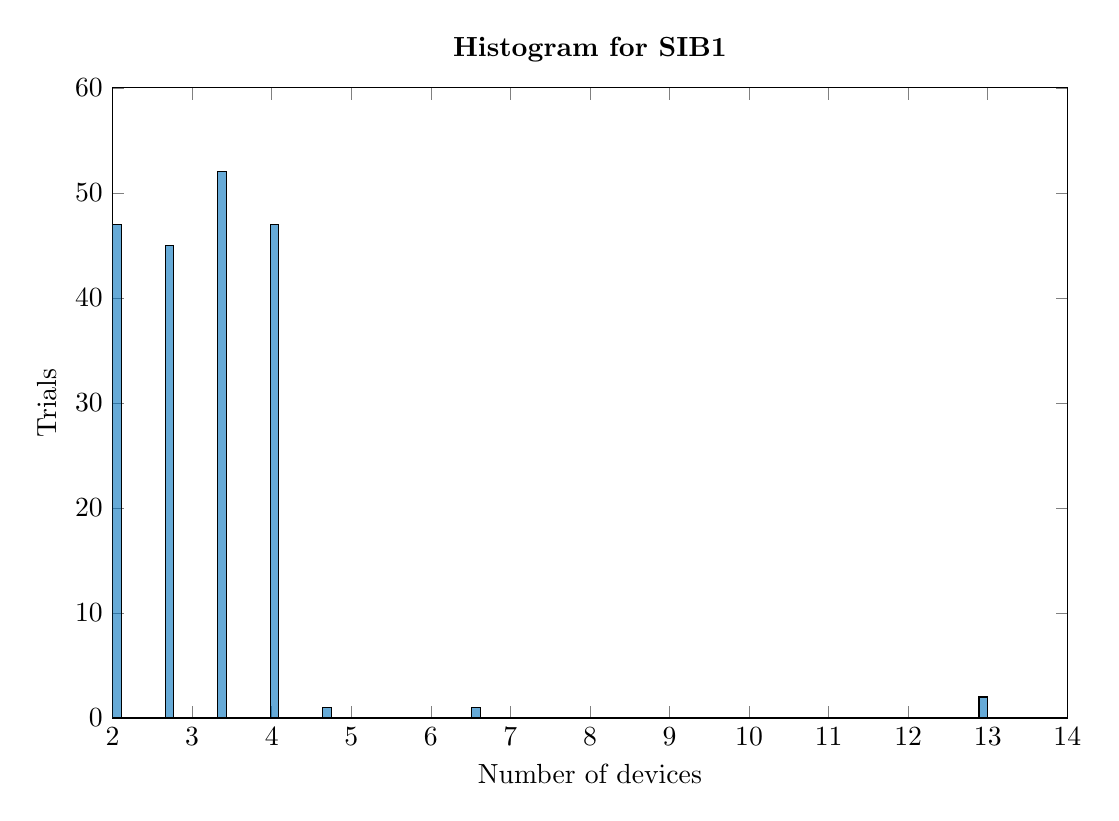
\begin{tikzpicture}

\begin{axis}[%
width=\textwidth,
height=0.66\textwidth,
at={(0.758in,0.481in)},
scale only axis,
xmin=2,
xmax=14,
xlabel={Number of devices},
ymin=0,
ymax=60,
ylabel={Trials},
axis background/.style={fill=white},
title style={font=\bfseries},
title={Histogram for SIB1}
]
\addplot[fill=mycolor1,fill opacity=0.6,draw=black,ybar interval,area legend] plot table[row sep=crcr] {%
x	y\\
2	47\\
2.11	0\\
2.22	0\\
2.33	0\\
2.44	0\\
2.55	0\\
2.66	45\\
2.77	0\\
2.88	0\\
2.99	0\\
3.1	0\\
3.21	0\\
3.32	52\\
3.43	0\\
3.54	0\\
3.65	0\\
3.76	0\\
3.87	0\\
3.98	47\\
4.09	0\\
4.2	0\\
4.31	0\\
4.42	0\\
4.53	0\\
4.64	1\\
4.75	0\\
4.86	0\\
4.97	0\\
5.08	0\\
5.19	0\\
5.3	0\\
5.41	0\\
5.52	0\\
5.63	0\\
5.74	0\\
5.85	0\\
5.96	0\\
6.07	0\\
6.18	0\\
6.29	0\\
6.4	0\\
6.51	1\\
6.62	0\\
6.73	0\\
6.84	0\\
6.95	0\\
7.06	0\\
7.17	0\\
7.28	0\\
7.39	0\\
7.5	0\\
7.61	0\\
7.72	0\\
7.83	0\\
7.94	0\\
8.05	0\\
8.16	0\\
8.27	0\\
8.38	0\\
8.49	0\\
8.6	0\\
8.71	0\\
8.82	0\\
8.93	0\\
9.04	0\\
9.15	0\\
9.26	0\\
9.37	0\\
9.48	0\\
9.59	0\\
9.7	0\\
9.81	0\\
9.92	0\\
10.03	0\\
10.14	0\\
10.25	0\\
10.36	0\\
10.47	0\\
10.58	0\\
10.69	0\\
10.8	0\\
10.91	0\\
11.02	0\\
11.13	0\\
11.24	0\\
11.35	0\\
11.46	0\\
11.57	0\\
11.68	0\\
11.79	0\\
11.9	0\\
12.01	0\\
12.12	0\\
12.23	0\\
12.34	0\\
12.45	0\\
12.56	0\\
12.67	0\\
12.78	0\\
12.89	2\\
13	2\\
};
\end{axis}
\end{tikzpicture}%}
\caption{Execution time for the decoding the NB-SIB1 step for different number of devices and the baseline emulator.}
\label{fig:MT_SIB1_His}
\end{figure}
\end{minipage}
\captionsetup{belowskip=-1.5em}

As seen on \autoref{fig:MT_SIB1_Time} the baseline emulator and the MDE have the same tendency around four different time values, with a few measurements way off. Compared to the previous steps, this step has a long execution time and the steps between the time values is around 600 ms. On \autoref{fig:MT_SIB1_His}  the distribution can be seen, where it is seen that the values is equally distributed between the four different time values. This indicates that the MDE begins the search at four different times, compared to the repeating of the NB-SIB1 message.
\todo{search? quite specific step size to be due to different start times}


\subsection{NB-SIB2}
The execution time for the NB-SIB2 decoding step is measured from the NB-SIB1 is decoded until NB-SIB2 is decoded, which gives the results seen on \autoref{fig:MT_SIB2_Time}. The transmission after NB-SIB1 error narrows the number of measurement points down even further for this step in the process.

\begin{figure}[H]
\tikzsetnextfilename{MT_SIB2_Time}
\centering
% This file was created by matlab2tikz.
%
%The latest updates can be retrieved from
%  http://www.mathworks.com/matlabcentral/fileexchange/22022-matlab2tikz-matlab2tikz
%where you can also make suggestions and rate matlab2tikz.
%
\definecolor{mycolor1}{rgb}{0.00000,0.44700,0.74100}%
\definecolor{mycolor2}{rgb}{0.85000,0.32500,0.09800}%
%
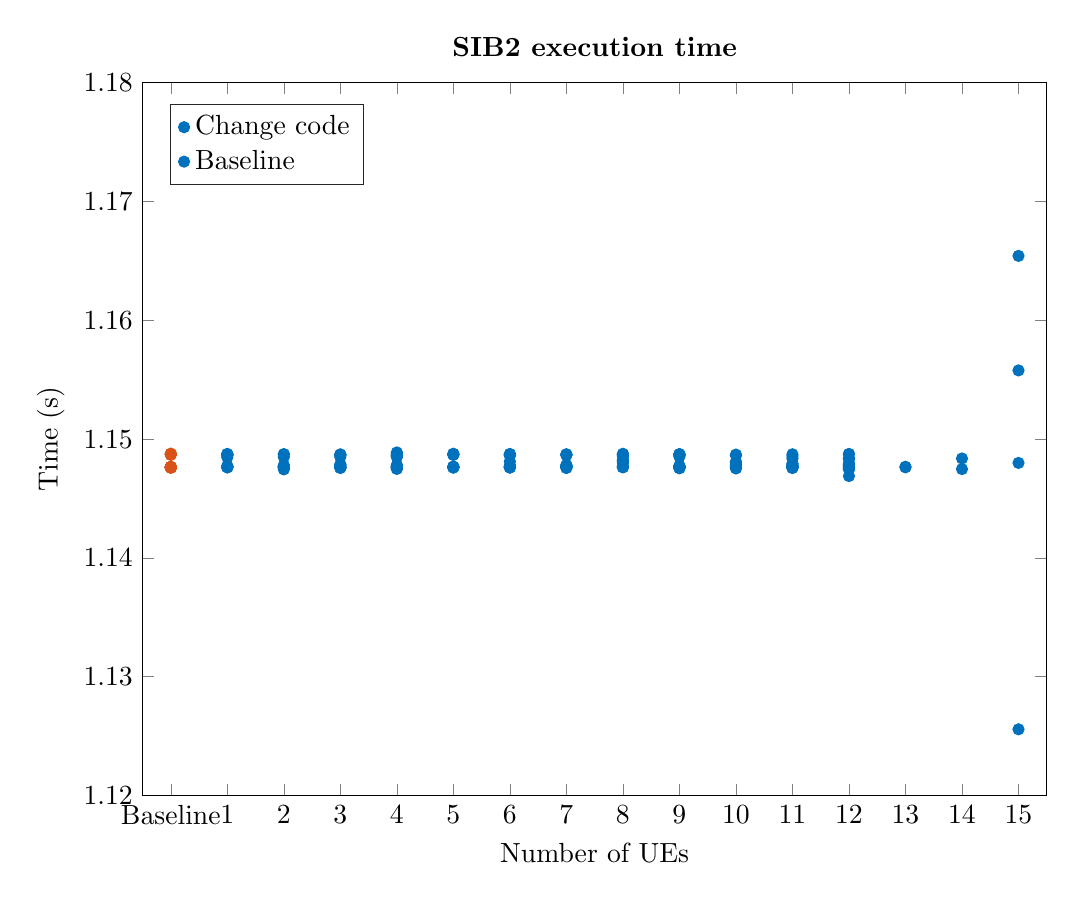
\begin{tikzpicture}

\begin{axis}[%
width=4.521in,
height=3.566in,
at={(0.758in,0.481in)},
scale only axis,
xmin=-0.5,
xmax=15.5,
xtick={0,1,2,3,4,5,6,7,8,9,10,11,12,13,14,15},
xticklabels={{Baseline},{1},{2},{3},{4},{5},{6},{7},{8},{9},{10},{11},{12},{13},{14},{15}},
xlabel={Number of UEs},
ymin=1.12,
ymax=1.18,
ylabel={Time (s)},
axis background/.style={fill=white},
title style={font=\bfseries},
title={SIB2 execution time},
legend style={at={(0.03,0.97)},anchor=north west,legend cell align=left,align=left,draw=white!15!black}
]
\addplot [color=mycolor1,only marks,mark=*,mark options={solid}]
  table[row sep=crcr]{%
1	1.14861416816711\\
1	1.14764595031738\\
1	1.14869999885559\\
1	1.14867520332336\\
1	1.14768314361572\\
1	1.14871907234192\\
1	1.14760398864746\\
1	0\\
1	1.14761400222778\\
1	0\\
1	0\\
1	1.14873504638672\\
1	1.14866995811462\\
1	1.14762902259827\\
1	1.14844989776611\\
1	1.14772701263428\\
1	1.14866614341736\\
1	1.14762902259827\\
1	1.14766502380371\\
1	0\\
};
\addlegendentry{Change code};

\addplot [color=mycolor1,only marks,mark=*,mark options={solid}]
  table[row sep=crcr]{%
2	0\\
2	1.14869999885559\\
2	1.14872193336487\\
2	1.14743685722351\\
2	1.14759993553162\\
2	1.1476469039917\\
2	0\\
2	0\\
2	1.14758086204529\\
2	1.14762592315674\\
2	1.14773392677307\\
2	0\\
2	0\\
2	0\\
2	1.14763808250427\\
2	0\\
2	1.14763689041138\\
2	1.14846801757813\\
2	1.14778089523315\\
2	0\\
};
\addlegendentry{Baseline};

\addplot [color=mycolor1,only marks,mark=*,mark options={solid},forget plot]
  table[row sep=crcr]{%
3	0\\
3	1.1484739780426\\
3	1.14770102500916\\
3	1.14761209487915\\
3	1.14775395393372\\
3	1.14868903160095\\
3	0\\
3	1.14869093894959\\
3	1.14865207672119\\
3	1.14784407615662\\
3	1.14785313606262\\
3	1.14755582809448\\
3	0\\
3	1.14864993095398\\
3	0\\
3	0\\
3	1.14760112762451\\
3	1.14760613441467\\
3	1.14757800102234\\
3	1.14759707450867\\
};
\addplot [color=mycolor1,only marks,mark=*,mark options={solid},forget plot]
  table[row sep=crcr]{%
4	1.14768004417419\\
4	1.14766192436218\\
4	1.1485378742218\\
4	0\\
4	0\\
4	1.14876699447632\\
4	1.14763498306274\\
4	1.14748001098633\\
4	1.14754796028137\\
4	0\\
4	1.14770913124084\\
4	1.14860796928406\\
4	1.14766693115234\\
4	1.14847683906555\\
4	1.14886403083801\\
4	1.14751315116882\\
4	1.14781403541565\\
4	1.14758896827698\\
4	1.14863586425781\\
4	1.14876008033752\\
};
\addplot [color=mycolor1,only marks,mark=*,mark options={solid},forget plot]
  table[row sep=crcr]{%
5	1.14869904518127\\
5	1.14763689041138\\
5	1.14762902259827\\
5	1.14758992195129\\
5	1.14868807792664\\
5	0\\
5	0\\
5	1.14759087562561\\
5	1.14765095710754\\
5	0\\
5	0\\
5	1.14874196052551\\
5	1.14760994911194\\
5	1.14874196052551\\
5	0\\
5	0\\
5	0\\
5	0\\
5	1.1476788520813\\
5	1.14865398406982\\
};
\addplot [color=mycolor1,only marks,mark=*,mark options={solid},forget plot]
  table[row sep=crcr]{%
6	1.14870095252991\\
6	1.14779305458069\\
6	1.14860796928406\\
6	1.14767384529114\\
6	1.14760899543762\\
6	1.14768695831299\\
6	0\\
6	1.14863681793213\\
6	1.14810705184937\\
6	1.1475830078125\\
6	1.14868903160095\\
6	0\\
6	1.14762282371521\\
6	1.1486439704895\\
6	0\\
6	1.14873480796814\\
6	0\\
6	0\\
6	1.14763402938843\\
6	1.14762711524963\\
};
\addplot [color=mycolor1,only marks,mark=*,mark options={solid},forget plot]
  table[row sep=crcr]{%
7	1.14771604537964\\
7	0\\
7	1.14766097068787\\
7	1.14756989479065\\
7	0\\
7	1.14763617515564\\
7	1.1486930847168\\
7	0\\
7	0\\
7	0\\
7	1.14779114723206\\
7	1.14769601821899\\
7	1.14865589141846\\
7	1.14863991737366\\
7	1.14755702018738\\
7	1.1476879119873\\
7	0\\
7	1.14870691299438\\
7	1.14779496192932\\
7	1.14769411087036\\
};
\addplot [color=mycolor1,only marks,mark=*,mark options={solid},forget plot]
  table[row sep=crcr]{%
8	1.14765310287476\\
8	1.14868092536926\\
8	1.148521900177\\
8	1.14763808250427\\
8	0\\
8	1.14762806892395\\
8	1.14874792098999\\
8	0\\
8	1.14770197868347\\
8	1.14808297157288\\
8	0\\
8	1.14866805076599\\
8	0\\
8	1.14819407463074\\
8	1.14826083183289\\
8	1.14760708808899\\
8	1.14861392974854\\
8	1.1487021446228\\
8	1.14819502830505\\
8	1.14798307418823\\
};
\addplot [color=mycolor1,only marks,mark=*,mark options={solid},forget plot]
  table[row sep=crcr]{%
9	0\\
9	1.14850616455078\\
9	1.14752793312073\\
9	1.14864087104797\\
9	1.14869999885559\\
9	0\\
9	1.14872694015503\\
9	1.14868307113647\\
9	1.14765501022339\\
9	1.14763712882996\\
9	1.14769601821899\\
9	1.14774680137634\\
9	0\\
9	1.14756488800049\\
9	1.14765596389771\\
9	1.14865112304688\\
9	1.14868903160095\\
9	1.14756202697754\\
9	1.14766097068787\\
9	1.14769601821899\\
};
\addplot [color=mycolor1,only marks,mark=*,mark options={solid},forget plot]
  table[row sep=crcr]{%
10	0\\
10	1.14868307113647\\
10	1.14751195907593\\
10	1.14756798744202\\
10	0\\
10	0\\
10	0\\
10	1.14770293235779\\
10	0\\
10	0\\
10	1.14860892295837\\
10	1.1476309299469\\
10	1.14767909049988\\
10	0\\
10	0\\
10	1.14785599708557\\
10	1.14808678627014\\
10	1.1480119228363\\
10	0\\
10	0\\
};
\addplot [color=mycolor1,only marks,mark=*,mark options={solid},forget plot]
  table[row sep=crcr]{%
11	1.1487090587616\\
11	1.14756202697754\\
11	1.14763712882996\\
11	1.14790201187134\\
11	0\\
11	1.14756107330322\\
11	1.14760112762451\\
11	1.14776301383972\\
11	1.14790391921997\\
11	1.14773893356323\\
11	1.14760589599609\\
11	1.14763593673706\\
11	0\\
11	0\\
11	1.14833998680115\\
11	0\\
11	0\\
11	0\\
11	1.14766192436218\\
11	1.1485481262207\\
};
\addplot [color=mycolor1,only marks,mark=*,mark options={solid},forget plot]
  table[row sep=crcr]{%
12	1.147705078125\\
12	1.14687490463257\\
12	1.14872598648071\\
12	1.14797592163086\\
12	1.14834499359131\\
12	1.14762115478516\\
12	1.14752197265625\\
12	0\\
12	0\\
12	0\\
12	1.14772891998291\\
12	1.14748311042786\\
12	1.14785885810852\\
12	0\\
12	1.14766788482666\\
12	1.14836406707764\\
12	1.1478488445282\\
12	1.14873003959656\\
12	1.14742994308472\\
12	1.14833402633667\\
};
\addplot [color=mycolor1,only marks,mark=*,mark options={solid},forget plot]
  table[row sep=crcr]{%
13	0\\
13	0\\
13	0\\
13	0\\
13	1.14760804176331\\
13	0\\
13	0\\
13	0\\
13	0\\
13	0\\
13	0\\
13	0\\
13	0\\
13	0\\
13	1.1476571559906\\
13	0\\
13	0\\
13	0\\
13	0\\
13	0\\
};
\addplot [color=mycolor1,only marks,mark=*,mark options={solid},forget plot]
  table[row sep=crcr]{%
14	0\\
14	0\\
14	0\\
14	0\\
14	0\\
14	0\\
14	0\\
14	1.14835405349731\\
14	0\\
14	0\\
14	1.14746284484863\\
14	0\\
14	0\\
14	0\\
14	0\\
14	0\\
14	0\\
14	0\\
14	0\\
14	0\\
};
\addplot [color=mycolor1,only marks,mark=*,mark options={solid},forget plot]
  table[row sep=crcr]{%
15	1.12556910514832\\
15	0\\
15	0\\
15	1.14798092842102\\
15	0\\
15	1.15576195716858\\
15	0\\
15	0\\
15	0\\
15	0\\
15	0\\
15	0\\
15	1.16539812088013\\
15	0\\
15	0\\
15	0\\
15	0\\
15	0\\
15	0\\
15	0\\
};
\addplot [color=mycolor2,only marks,mark=*,mark options={solid},forget plot]
  table[row sep=crcr]{%
0	1.14874005317688\\
0	0\\
0	1.1475682258606\\
0	1.14761090278625\\
0	1.14760684967041\\
0	1.14865493774414\\
0	1.14760994911194\\
0	0\\
0	1.14760112762451\\
0	1.14764499664307\\
0	1.14870381355286\\
0	1.14764499664307\\
0	1.1476149559021\\
0	1.14760780334473\\
0	1.14760398864746\\
0	1.14765095710754\\
0	1.14761114120483\\
0	1.14876103401184\\
0	1.14763188362122\\
0	1.14761209487915\\
};
\end{axis}
\end{tikzpicture}%
\caption{Execution time for the decoding the NB-SIB2 step for different number of devices and the baseline emulator.}
\label{fig:MT_SIB2_Time}
\end{figure}


As seen on \autoref{fig:MT_SIB2_Time}, the baseline emulator and MDE have the same tendency, beside for when there is emulated 15 devices. There is not a big spread for the measurements of 1 through 14 devices, which is also expected as the timing between decoding NB-SIB1 and NB-SIB2 should only be the time until the whole NB-SIB2 have been received, with a small additional time for the decoding. 
\todo{explain why 15 is weird}


\subsection{NPRACH}
The execution time for the NPRACH step is measured from the decoding of NB-SIB2 is done until the msg1 is delivered to the transmit buffer, which gives the results seen on \autoref{fig:MT_Nprach_Time}. The NPRACH error occurs only when the MDE emulates more than 12 devices with a single exception. The NPRACH error happens, when only some of the devices get through the NPRACH step. As before the shown results are only for one of the emulated devices and the sample pool is not reduced by this error.
\todo{mads bør læse det her igen}

\begin{figure}[H]
\tikzsetnextfilename{MT_Nprach_Time}
\centering
\resizebox{0.5\textwidth}{!}{
% This file was created by matlab2tikz.
%
%The latest updates can be retrieved from
%  http://www.mathworks.com/matlabcentral/fileexchange/22022-matlab2tikz-matlab2tikz
%where you can also make suggestions and rate matlab2tikz.
%
\definecolor{mycolor1}{rgb}{0.00000,0.44700,0.74100}%
\definecolor{mycolor2}{rgb}{0.85000,0.32500,0.09800}%
%
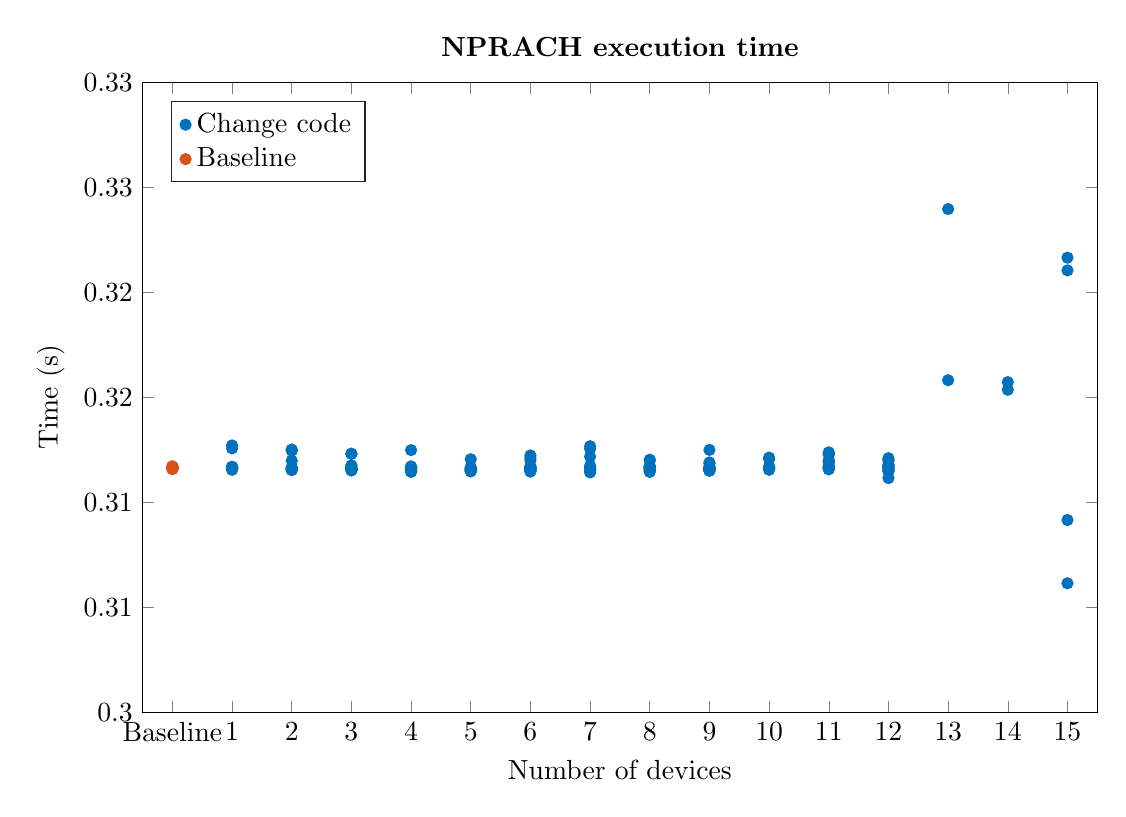
\begin{tikzpicture}

\begin{axis}[%
width=\textwidth,
height=.66\textwidth,
at={(0.758in,0.481in)},
scale only axis,
xmin=-0.5,
xmax=15.5,
xtick={0,1,2,3,4,5,6,7,8,9,10,11,12,13,14,15},
xticklabels={{Baseline},{1},{2},{3},{4},{5},{6},{7},{8},{9},{10},{11},{12},{13},{14},{15}},
xlabel={Number of devices},
ymin=0.3,
ymax=0.33,
ylabel={Time (s)},
axis background/.style={fill=white},
title style={font=\bfseries},
title={NPRACH execution time},
legend style={at={(0.03,0.97)},anchor=north west,legend cell align=left,align=left,draw=white!15!black}
]
\addplot [color=mycolor1,only marks,mark=*,mark options={solid}]
  table[row sep=crcr]{%
1	0.311680793762207\\
1	0.311604022979736\\
1	0.311627864837646\\
1	0.311679840087891\\
1	0.311601877212524\\
1	0.311666011810303\\
1	0.311678886413574\\
1	0\\
1	0.311702966690063\\
1	0\\
1	0\\
1	0.311586856842041\\
1	0.311655044555664\\
1	0.311685085296631\\
1	0.311557054519653\\
1	0.312576055526733\\
1	0.311637878417969\\
1	0.312717914581299\\
1	0.311601161956787\\
1	0\\
};
\addlegendentry{Change code};

\addplot [color=mycolor1,only marks,mark=*,mark options={solid},forget plot]
  table[row sep=crcr]{%
2	0\\
2	0.311550140380859\\
2	0.311643123626709\\
2	0.31199312210083\\
2	0.311596870422363\\
2	0.31159496307373\\
2	0\\
2	0\\
2	0.311676025390625\\
2	0.311542987823486\\
2	0.312494993209839\\
2	0\\
2	0\\
2	0\\
2	0.311656951904297\\
2	0\\
2	0.312523126602173\\
2	0.311601877212524\\
2	0.312467098236084\\
2	0\\
};


\addplot [color=mycolor1,only marks,mark=*,mark options={solid},forget plot]
  table[row sep=crcr]{%
3	0\\
3	0.311551809310913\\
3	0.311765193939209\\
3	0.311564922332764\\
3	0.311563014984131\\
3	0.311522006988525\\
3	0\\
3	0.311599016189575\\
3	0.311592102050781\\
3	0.312321901321411\\
3	0.312319040298462\\
3	0.311748027801514\\
3	0\\
3	0.311631202697754\\
3	0\\
3	0\\
3	0.31165599822998\\
3	0.311599969863892\\
3	0.311576128005981\\
3	0.311599969863892\\
};
\addplot [color=mycolor1,only marks,mark=*,mark options={solid},forget plot]
  table[row sep=crcr]{%
4	0.311563014984131\\
4	0.311460018157959\\
4	0.311659097671509\\
4	0\\
4	0\\
4	0.311501979827881\\
4	0.311540126800537\\
4	0.311670064926147\\
4	0.31163501739502\\
4	0\\
4	0.311506986618042\\
4	0.311635971069336\\
4	0.31148099899292\\
4	0.311570167541504\\
4	0.311554193496704\\
4	0.311676979064941\\
4	0.312494039535522\\
4	0.311719179153442\\
4	0.311642169952393\\
4	0.311550855636597\\
};
\addplot [color=mycolor1,only marks,mark=*,mark options={solid},forget plot]
  table[row sep=crcr]{%
5	0.311535835266113\\
5	0.311478137969971\\
5	0.312060117721558\\
5	0.311666011810303\\
5	0.311637878417969\\
5	0\\
5	0\\
5	0.311530113220215\\
5	0.311499834060669\\
5	0\\
5	0\\
5	0.31154990196228\\
5	0.311671018600464\\
5	0.311539888381958\\
5	0\\
5	0\\
5	0\\
5	0\\
5	0.311614990234375\\
5	0.311556816101074\\
};
\addplot [color=mycolor1,only marks,mark=*,mark options={solid},forget plot]
  table[row sep=crcr]{%
6	0.311546087265015\\
6	0.311470031738281\\
6	0.311733961105347\\
6	0.311630010604858\\
6	0.312007188796997\\
6	0.311566114425659\\
6	0\\
6	0.311662197113037\\
6	0.31212592124939\\
6	0.3122398853302\\
6	0.311693906784058\\
6	0\\
6	0.311550140380859\\
6	0.311647891998291\\
6	0\\
6	0.311639070510864\\
6	0\\
6	0\\
6	0.311668872833252\\
6	0.311506032943726\\
};
\addplot [color=mycolor1,only marks,mark=*,mark options={solid},forget plot]
  table[row sep=crcr]{%
7	0.312558889389038\\
7	0\\
7	0.311611890792847\\
7	0.311638116836548\\
7	0\\
7	0.311750888824463\\
7	0.31158185005188\\
7	0\\
7	0\\
7	0\\
7	0.311608791351318\\
7	0.311516046524048\\
7	0.31172513961792\\
7	0.311556100845337\\
7	0.312680959701538\\
7	0.311551094055176\\
7	0\\
7	0.311511039733887\\
7	0.311432123184204\\
7	0.312183856964111\\
};
\addplot [color=mycolor1,only marks,mark=*,mark options={solid},forget plot]
  table[row sep=crcr]{%
8	0.311455965042114\\
8	0.311665058135986\\
8	0.311743974685669\\
8	0.311501026153564\\
8	0\\
8	0.311676025390625\\
8	0.311566114425659\\
8	0\\
8	0.311695098876953\\
8	0.311681032180786\\
8	0\\
8	0.311643838882446\\
8	0\\
8	0.312039852142334\\
8	0.31199312210083\\
8	0.311548948287964\\
8	0.311679840087891\\
8	0.311714887619019\\
8	0.31155800819397\\
8	0.311631917953491\\
};
\addplot [color=mycolor1,only marks,mark=*,mark options={solid},forget plot]
  table[row sep=crcr]{%
9	0\\
9	0.311545848846436\\
9	0.311694145202637\\
9	0.31157112121582\\
9	0.311569929122925\\
9	0\\
9	0.31165599822998\\
9	0.311696767807007\\
9	0.311599969863892\\
9	0.311621904373169\\
9	0.311509132385254\\
9	0.311530113220215\\
9	0\\
9	0.312504053115845\\
9	0.311852216720581\\
9	0.311555862426758\\
9	0.311640977859497\\
9	0.311907052993774\\
9	0.311527013778687\\
9	0.311538934707642\\
};
\addplot [color=mycolor1,only marks,mark=*,mark options={solid},forget plot]
  table[row sep=crcr]{%
10	0\\
10	0.311673879623413\\
10	0.311647891998291\\
10	0.311652898788452\\
10	0\\
10	0\\
10	0\\
10	0.311555862426758\\
10	0\\
10	0\\
10	0.31167197227478\\
10	0.312138080596924\\
10	0.31160306930542\\
10	0\\
10	0\\
10	0.312062978744507\\
10	0.311703205108643\\
10	0.311650991439819\\
10	0\\
10	0\\
};
\addplot [color=mycolor1,only marks,mark=*,mark options={solid},forget plot]
  table[row sep=crcr]{%
11	0.311681032180786\\
11	0.31174898147583\\
11	0.311945915222168\\
11	0.312388181686401\\
11	0\\
11	0.311898946762085\\
11	0.311634063720703\\
11	0.312273979187012\\
11	0.31233811378479\\
11	0.311637878417969\\
11	0.311670064926147\\
11	0.311576128005981\\
11	0\\
11	0\\
11	0.312019824981689\\
11	0\\
11	0\\
11	0\\
11	0.311609029769897\\
11	0.311727046966553\\
};
\addplot [color=mycolor1,only marks,mark=*,mark options={solid},forget plot]
  table[row sep=crcr]{%
12	0.311507940292358\\
12	0.311978101730347\\
12	0.311573028564453\\
12	0.311161041259766\\
12	0.312034130096436\\
12	0.311545848846436\\
12	0.311670064926147\\
12	0\\
12	0\\
12	0\\
12	0.311485052108765\\
12	0.311722993850708\\
12	0.311711072921753\\
12	0\\
12	0.31154990196228\\
12	0.311701059341431\\
12	0.31179404258728\\
12	0.311655044555664\\
12	0.311732053756714\\
12	0.312110900878906\\
};
\addplot [color=mycolor1,only marks,mark=*,mark options={solid},forget plot]
  table[row sep=crcr]{%
13	0\\
13	0\\
13	0\\
13	0\\
13	0.315821886062622\\
13	0\\
13	0\\
13	0\\
13	0\\
13	0\\
13	0\\
13	0\\
13	0\\
13	0\\
13	0.323969841003418\\
13	0\\
13	0\\
13	0\\
13	0\\
13	0\\
};
\addplot [color=mycolor1,only marks,mark=*,mark options={solid},forget plot]
  table[row sep=crcr]{%
14	0\\
14	0\\
14	0\\
14	0\\
14	0\\
14	0\\
14	0\\
14	0.315366983413696\\
14	0\\
14	0\\
14	0.315733194351196\\
14	0\\
14	0\\
14	0\\
14	0\\
14	0\\
14	0\\
14	0\\
14	0\\
14	0\\
};
\addplot [color=mycolor1,only marks,mark=*,mark options={solid},forget plot]
  table[row sep=crcr]{%
15	0.309165954589844\\
15	0\\
15	0\\
15	0.321655988693237\\
15	0\\
15	0.306154012680054\\
15	0\\
15	0\\
15	0\\
15	0\\
15	0\\
15	0\\
15	0.321050882339478\\
15	0\\
15	0\\
15	0\\
15	0\\
15	0\\
15	0\\
15	0\\
};
\addplot [color=mycolor2,only marks,mark=*,mark options={solid}]
  table[row sep=crcr]
\caption{Execution time for the NPRACH step for different number of devices and the baseline emulator.}
\label{fig:MT_Nprach_Time}
\end{figure}

As seen on \autoref{fig:MT_Nprach_Time} the baseline emulator and MDE takes approximately the same time, but the MDE has a bigger spread of its measurement points. All the measurements of the MDE with more than 12 devices, does not follow the tendency of the other measurements. This should come from the fact, that all the shown measurement points for these number of devices, is measurements where the NPRACH error occurred and none of them made it error free through, as seen on \autoref{fig:MT_error_dist}.

\subsection{RAR}
The execution time for the RAR step is measured from msg1 is delivered to the transmit buffer until msg2 is received, which gives the results seen on \autoref{fig:MT_Rar_Time}. The msg2 error occurs here, if no msg2 is received and the measurements are therefore excluded. 

\begin{figure}[H]
\tikzsetnextfilename{MT_Rar_Time}
\centering
\resizebox{0.5\textwidth}{!}{
% This file was created by matlab2tikz.
%
%The latest updates can be retrieved from
%  http://www.mathworks.com/matlabcentral/fileexchange/22022-matlab2tikz-matlab2tikz
%where you can also make suggestions and rate matlab2tikz.
%
\definecolor{mycolor1}{rgb}{0.00000,0.44700,0.74100}%
\definecolor{mycolor2}{rgb}{0.85000,0.32500,0.09800}%
%
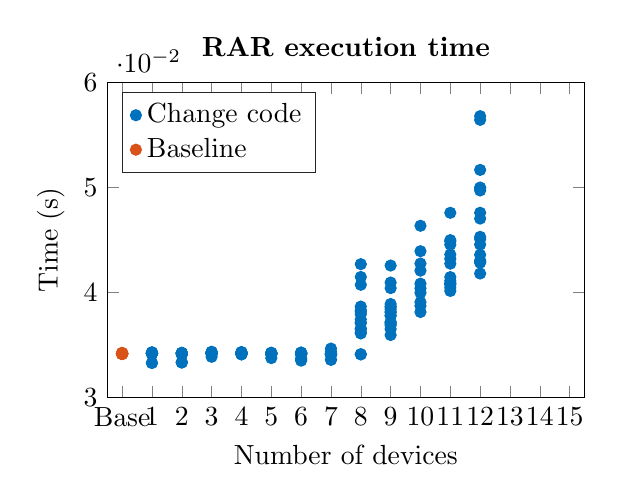
\begin{tikzpicture}

\begin{axis}[%
width=.5\textwidth,
height=.33\textwidth,
at={(0.758in,0.481in)},
scale only axis,
xmin=-0.5,
xmax=15.5,
xtick={0,1,2,3,4,5,6,7,8,9,10,11,12,13,14,15},
xticklabels={{Base},{1},{2},{3},{4},{5},{6},{7},{8},{9},{10},{11},{12},{13},{14},{15}},
xlabel={Number of devices},
ymin=0.03,
ymax=0.06,
ylabel={Time (s)},
axis background/.style={fill=white},
title style={font=\bfseries},
title={RAR execution time},
legend style={at={(0.03,0.97)},anchor=north west,legend cell align=left,align=left,draw=white!15!black}
]
\addplot [color=mycolor1,only marks,mark=*,mark options={solid}]
  table[row sep=crcr]{%
1	0.0341880321502686\\
1	0.034235954284668\\
1	0.0342159271240234\\
1	0.0342271327972412\\
1	0.0342719554901123\\
1	0.0341730117797852\\
1	0\\
1	0\\
1	0.0341699123382568\\
1	0\\
1	0\\
1	0.0342731475830078\\
1	0.0341849327087402\\
1	0.0341880321502686\\
1	0.0343189239501953\\
1	0.0333008766174316\\
1	0.0342051982879639\\
1	0.033297061920166\\
1	0.0342288017272949\\
1	0\\
};
\addlegendentry{Change code};

\addplot [color=mycolor1,only marks,mark=*,mark options={solid},forget plot]
  table[row sep=crcr]{%
2	0\\
2	0.0342118740081787\\
2	0.0341849327087402\\
2	0.0340640544891357\\
2	0.0342371463775635\\
2	0.0342140197753906\\
2	0\\
2	0\\
2	0.0341610908508301\\
2	0.0342671871185303\\
2	0.0333490371704102\\
2	0\\
2	0\\
2	0\\
2	0.0342299938201904\\
2	0\\
2	0.0333659648895264\\
2	0.0342400074005127\\
2	0.0333349704742432\\
2	0\\
};

\addplot [color=mycolor1,only marks,mark=*,mark options={solid},forget plot]
  table[row sep=crcr]{%
3	0\\
3	0.0342600345611572\\
3	0.0338799953460693\\
3	0.0342161655426025\\
3	0.0342400074005127\\
3	0.0343279838562012\\
3	0\\
3	0.0342199802398682\\
3	0.0342228412628174\\
3	0.0342550277709961\\
3	0.0343589782714844\\
3	0.0341391563415527\\
3	0\\
3	0.0343039035797119\\
3	0\\
3	0\\
3	0.0342159271240234\\
3	0.03420090675354\\
3	0.0342509746551514\\
3	0.0342059135437012\\
};
\addplot [color=mycolor1,only marks,mark=*,mark options={solid},forget plot]
  table[row sep=crcr]{%
4	0.0342638492584229\\
4	0.0343360900878906\\
4	0.0341908931732178\\
4	0\\
4	0\\
4	0.0342490673065186\\
4	0.0342738628387451\\
4	0.0342228412628174\\
4	0.0341949462890625\\
4	0\\
4	0.0342400074005127\\
4	0.0342440605163574\\
4	0.0342991352081299\\
4	0.0341489315032959\\
4	0.0341489315032959\\
4	0.0342459678649902\\
4	0.0341918468475342\\
4	0.0341000556945801\\
4	0.034153938293457\\
4	0.034203052520752\\
};
\addplot [color=mycolor1,only marks,mark=*,mark options={solid},forget plot]
  table[row sep=crcr]{%
5	0.0342710018157959\\
5	0.0341567993164063\\
5	0.0337579250335693\\
5	0.0341598987579346\\
5	0.0341479778289795\\
5	0\\
5	0\\
5	0.0342059135437012\\
5	0.0342340469360352\\
5	0\\
5	0\\
5	0.0342390537261963\\
5	0.0341389179229736\\
5	0.0341851711273193\\
5	0\\
5	0\\
5	0\\
5	0\\
5	0.034188985824585\\
5	0.0342321395874023\\
};
\addplot [color=mycolor1,only marks,mark=*,mark options={solid},forget plot]
  table[row sep=crcr]{%
6	0.0342798233032227\\
6	0.0341129302978516\\
6	0.0341250896453857\\
6	0.0342040061950684\\
6	0.0337188243865967\\
6	0.0342609882354736\\
6	0\\
6	0.0342237949371338\\
6	0.0336298942565918\\
6	0.0335140228271484\\
6	0.0341589450836182\\
6	0\\
6	0.0342769622802734\\
6	0.0342199802398682\\
6	0\\
6	0.0342271327972412\\
6	0\\
6	0\\
6	0.0341720581054688\\
6	0\\
};
\addplot [color=mycolor1,only marks,mark=*,mark options={solid},forget plot]
  table[row sep=crcr]{%
7	0.0336170196533203\\
7	0\\
7	0.0341181755065918\\
7	0.0341799259185791\\
7	0\\
7	0.0342490673065186\\
7	0.0342171192169189\\
7	0\\
7	0\\
7	0\\
7	0.0346660614013672\\
7	0.0343749523162842\\
7	0.0340960025787354\\
7	0.0341479778289795\\
7	0.0340781211853027\\
7	0.0341360569000244\\
7	0\\
7	0.0341110229492188\\
7	0.034153938293457\\
7	0.0335919857025146\\
};
\addplot [color=mycolor1,only marks,mark=*,mark options={solid},forget plot]
  table[row sep=crcr]{%
8	0.0365910530090332\\
8	0.0427010059356689\\
8	0.0370931625366211\\
8	0.0381538867950439\\
8	0\\
8	0.0364658832550049\\
8	0.0379340648651123\\
8	0\\
8	0.0374419689178467\\
8	0.0407381057739258\\
8	0\\
8	0.0341041088104248\\
8	0\\
8	0.0414822101593018\\
8	0.0361030101776123\\
8	0.0386650562286377\\
8	0.0383260250091553\\
8	0.0362110137939453\\
8	0.0341310501098633\\
8	0.037121057510376\\
};
\addplot [color=mycolor1,only marks,mark=*,mark options={solid},forget plot]
  table[row sep=crcr]{%
9	0\\
9	0.0370240211486816\\
9	0.0365219116210938\\
9	0.0378210544586182\\
9	0.038114070892334\\
9	0\\
9	0.037787914276123\\
9	0.0381491184234619\\
9	0.0389068126678467\\
9	0.0386679172515869\\
9	0.0383989810943604\\
9	0.0359559059143066\\
9	0\\
9	0.042572021484375\\
9	0.0371799468994141\\
9	0.0409531593322754\\
9	0.0386199951171875\\
9	0.0404210090637207\\
9	0.036876916885376\\
9	0.0371849536895752\\
};
\addplot [color=mycolor1,only marks,mark=*,mark options={solid},forget plot]
  table[row sep=crcr]{%
10	0\\
10	0.0420839786529541\\
10	0.0408451557159424\\
10	0.0439350605010986\\
10	0\\
10	0\\
10	0\\
10	0.0399701595306396\\
10	0\\
10	0\\
10	0.0381450653076172\\
10	0.0463569164276123\\
10	0.0390889644622803\\
10	0\\
10	0\\
10	0.0403990745544434\\
10	0.0427589416503906\\
10	0.0387308597564697\\
10	0\\
10	0\\
};
\addplot [color=mycolor1,only marks,mark=*,mark options={solid},forget plot]
  table[row sep=crcr]{%
11	0.0449898242950439\\
11	0.0432069301605225\\
11	0.0445609092712402\\
11	0.0408809185028076\\
11	0\\
11	0.0404579639434814\\
11	0.0427489280700684\\
11	0.0475912094116211\\
11	0.0448739528656006\\
11	0.0414700508117676\\
11	0.0436179637908936\\
11	0.0411219596862793\\
11	0\\
11	0\\
11	0.0407330989837646\\
11	0\\
11	0\\
11	0\\
11	0.0408778190612793\\
11	0.040151834487915\\
};
\addplot [color=mycolor1,only marks,mark=*,mark options={solid},forget plot]
  table[row sep=crcr]{%
12	0.0453028678894043\\
12	0.0516760349273682\\
12	0.0564429759979248\\
12	0.0475959777832031\\
12	0.0430538654327393\\
12	0.0450849533081055\\
12	0.0470409393310547\\
12	0\\
12	0\\
12	0\\
12	0.0429530143737793\\
12	0.0567960739135742\\
12	0.0497169494628906\\
12	0\\
12	0.0499541759490967\\
12	0.0428369045257568\\
12	0.0435919761657715\\
12	0.0445668697357178\\
12	0.0499989986419678\\
12	0.0418119430541992\\
};
\addplot [color=mycolor1,only marks,mark=*,mark options={solid},forget plot]
  table[row sep=crcr]{%
13	0\\
13	0\\
13	0\\
13	0\\
13	0\\
13	0\\
13	0\\
13	0\\
13	0\\
13	0\\
13	0\\
13	0\\
13	0\\
13	0\\
13	0\\
13	0\\
13	0\\
13	0\\
13	0\\
13	0\\
};
\addplot [color=mycolor1,only marks,mark=*,mark options={solid},forget plot]
  table[row sep=crcr]{%
14	0\\
14	0\\
14	0\\
14	0\\
14	0\\
14	0\\
14	0\\
14	0\\
14	0\\
14	0\\
14	0\\
14	0\\
14	0\\
14	0\\
14	0\\
14	0\\
14	0\\
14	0\\
14	0\\
14	0\\
};
\addplot [color=mycolor1,only marks,mark=*,mark options={solid},forget plot]
  table[row sep=crcr]{%
15	0\\
15	0\\
15	0\\
15	0\\
15	0\\
15	0\\
15	0\\
15	0\\
15	0\\
15	0\\
15	0\\
15	0\\
15	0\\
15	0\\
15	0\\
15	0\\
15	0\\
15	0\\
15	0\\
15	0\\
};
\addplot [color=mycolor2,only marks,mark=*,mark options={solid}]
  table[row sep=crcr]
\caption{Execution time for the decoding the MIB-NB for different number of devices and the baseline emulator. A single measurement for the baseline is placed at 5.0834 s, which is not shown on this figure.}
\label{fig:MT_Rar_Time}
\end{figure}

As seen on \autoref{fig:MT_Rar_Time} the MDE starts out following the tendency of the baseline emulator, but around eight devices it begins to get a higher and higher execution time and getting a wider spread compared to the values at a low number of devices, which indicates a possible bottleneck in the system.

\subsection{Summary}
When looking at the execution time, of the MDE compared to the baseline emulator, it can be seen that in most steps, the two emulators perform similarly. The initialization steps is where the biggest difference is, but as the extra is performed in a single thread, this is to be expected. This is however not a problem as the real time dependency of the system has not yet been invoked. A bottleneck that can be seen in these test, comes in the RAR step, where an increase in delay is seen, when the number of number of devices gets above eight. The results from 13 to 15 device do act as the other measurements, but with no successful runs, is this expected as well. \todo{what do you mean, with the last part}


\section{CPU usage}
To test the CPU usage of the MDE, the test is split up into different steps as discussed in \autoref{sub:MassStruct}. 

The results is shown as average CPU usage over the steps time period, as the executing time is not equal for all measurement. The errors mentioned thorughout \autoref{sec:exeTime} is also effecting the CPU measurements and the measurement points, which have an error is removed from the sample pool for all consecutive steps.

The sample rate is 3 Hz, this is a rather slow sample rate, compared to the execution time for the different steps. This is the highest sample rate of any tool tested. The time window for the RAR step is unfortunately too small to be measured with a 3 Hz sample rate. The tool can not distinguish between individual cores of the PC and adds the usage together. In \appref{app:PC_stat} the number of cores in the PC is shown to be 8. A conservative estimation is made, that only 7 of these is available for the MDE, with the final 1 running background programs on the PC. 

\subsection{Initialization}
The initialization step is measured from the start of the emulator to the cell search begin. The average CPU usage of the MDE and baseline emulator can be seen on \autoref{fig:CPU_init}.

\begin{figure}[H]
\tikzsetnextfilename{CPU_init}
\centering
\resizebox{0.5\textwidth}{!}{
% This file was created by matlab2tikz.
%
%The latest updates can be retrieved from
%  http://www.mathworks.com/matlabcentral/fileexchange/22022-matlab2tikz-matlab2tikz
%where you can also make suggestions and rate matlab2tikz.
%
\definecolor{mycolor1}{rgb}{0.00000,0.44700,0.74100}%
\definecolor{mycolor2}{rgb}{0.85000,0.32500,0.09800}%
%
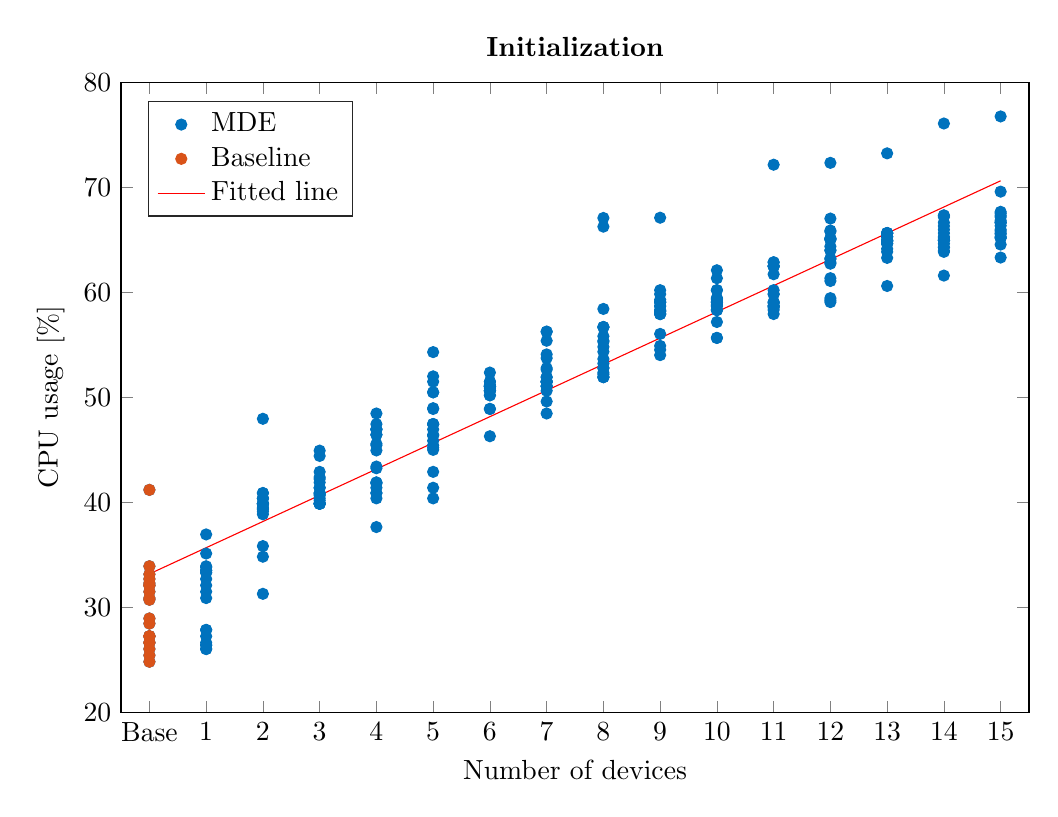
\begin{tikzpicture}

\begin{axis}[%
width=0.951\textwidth,
height=0.66\textwidth,
at={(0\textwidth,0\textwidth)},
scale only axis,
xmin=-0.5,
xmax=15.5,
xtick={0,1,2,3,4,5,6,7,8,9,10,11,12,13,14,15},
xticklabels={{Base},{1},{2},{3},{4},{5},{6},{7},{8},{9},{10},{11},{12},{13},{14},{15}},
xlabel={Number of devices},
ymin=20,
ymax=80,
ylabel={CPU usage [\%]},
axis background/.style={fill=white},
title style={font=\bfseries},
title={Initialization},
legend style={at={(0.03,0.97)},anchor=north west,legend cell align=left,align=left,draw=white!15!black},
y tick label style={/pgf/number format/fixed}
]
\addplot [color=mycolor1,only marks,mark=*,mark options={solid}]
  table[row sep=crcr]{%
0	32.12\\
1	35.15\\
2	39.5416666666667\\
3	40.9083333333333\\
4	37.67\\
5	48.9883333333333\\
6	51.0814285714286\\
7	49.6285714285714\\
8	55.8428571428571\\
9	58.18875\\
10	59.08875\\
11	58.71125\\
12	65.15\\
13	65.6566666666667\\
14	64.9822222222222\\
15	67.5488888888889\\
0	24.848\\
1	26.058\\
2	39.8983333333333\\
3	40.195\\
4	41.815\\
5	46.36\\
6	51.0828571428572\\
7	53.7571428571429\\
8	67.1\\
9	60.225\\
10	58.3325\\
11	62.51125\\
12	65.1725\\
13	65.3188888888889\\
14	65.3188888888889\\
15	65.8544444444444\\
0	41.21\\
1	26.434\\
2	40.9066666666667\\
3	41.9166666666667\\
4	46.465\\
5	48.9157142857143\\
6	48.9157142857143\\
7	52.8114285714286\\
8	56.7085714285714\\
9	59.3125\\
10	59.46875\\
11	62.87875\\
12	65.9075\\
13	60.6244444444444\\
14	64.9822222222222\\
15	65.6544444444444\\
0	28.484\\
1	26.416\\
2	40.9066666666667\\
3	42.9266666666667\\
4	46.9683333333333\\
5	40.4016666666667\\
6	51.5142857142857\\
7	51.0814285714286\\
8	51.9457142857143\\
9	56.06\\
10	59.08875\\
11	59.09\\
12	61.1\\
13	64.9811111111111\\
14	66.6666666666667\\
15	66.363\\
0	27.27\\
1	33.562\\
2	39.8966666666667\\
3	39.8966666666667\\
4	40.9066666666667\\
5	54.3285714285714\\
6	50.6485714285714\\
7	51.08\\
8	51.9457142857143\\
9	59.84625\\
10	60.225\\
11	57.95375\\
12	65.05\\
13	64.6455555555555\\
14	66.33\\
15	65.17\\
0	30.748\\
1	32.726\\
2	35.8566666666667\\
3	41.4116666666667\\
4	41.4116666666667\\
5	45.4533333333333\\
6	50.9157142857143\\
7	48.4828571428571\\
8	66.2728571428571\\
9	57.95375\\
10	59.09125\\
11	58.99\\
12	72.34875\\
13	64.6444444444444\\
14	67.34\\
15	76.7688888888889\\
0	33.172\\
1	26.058\\
2	34.8466666666667\\
3	40.67\\
4	46.9683333333333\\
5	46.9683333333333\\
6	50.6471428571429\\
7	51.5128571428571\\
8	52.8128571428571\\
9	57.95375\\
10	60.225\\
11	61.7425\\
12	67.04375\\
13	64.8744444444445\\
14	65.6555555555556\\
15	65.3177777777778\\
0	26.058\\
1	33.3316666666667\\
2	47.9783333333333\\
3	39.8983333333333\\
4	40.9066666666667\\
5	45.02\\
6	50.2157142857143\\
7	51.9457142857143\\
8	55.41\\
9	58.33125\\
10	59.32375\\
11	59.8475\\
12	65.79625\\
13	65.3188888888889\\
14	64.9811111111111\\
15	65.24\\
0	32.334\\
1	31.514\\
2	39.8233333333333\\
3	44.4416666666667\\
4	43.2683333333333\\
5	42.9266666666667\\
6	50.6471428571429\\
7	51.0814285714286\\
8	52.3785714285714\\
9	58.71125\\
10	58.7225\\
11	58.3425\\
12	64.01375\\
13	64.9822222222222\\
14	67.34\\
15	67.34\\
0	31.514\\
1	26.664\\
2	31.3116666666667\\
3	42.4216666666667\\
4	45.6016666666667\\
5	50.5033333333333\\
6	51.0814285714286\\
7	50.6471428571429\\
8	55.30125\\
9	58.19875\\
10	59.4675\\
11	58.56625\\
12	59.4675\\
13	63.8733333333333\\
14	64.6466666666667\\
15	65.9933333333333\\
0	32.726\\
1	33.332\\
2	40.4016666666667\\
3	42.2433333333333\\
4	48.4833333333333\\
5	46.4633333333333\\
6	50.2142857142857\\
7	51.5142857142857\\
8	56.7214285714286\\
9	58.71\\
10	58.71\\
11	59.09\\
12	59.2588888888889\\
13	65.6566666666667\\
14	67.1911111111111\\
15	69.6066666666667\\
0	30.908\\
1	36.968\\
2	40.4016666666667\\
3	39.8983333333333\\
4	40.4033333333333\\
5	47.4733333333333\\
6	52.38\\
7	56.2757142857143\\
8	52.8114285714286\\
9	59.09\\
10	62.12125\\
11	60.22625\\
12	63.17875\\
13	65.6566666666667\\
14	61.6144444444444\\
15	63.333\\
0	27.27\\
1	27.876\\
2	40.4016666666667\\
3	39.8966666666667\\
4	41.9166666666667\\
5	50.4942857142857\\
6	51.0814285714286\\
7	51.9457142857143\\
8	53.2442857142857\\
9	54.9225\\
10	58.3325\\
11	72.17125\\
12	62.745\\
13	65.3188888888889\\
14	64.3077777777778\\
15	64.5666666666667\\
0	27.27\\
1	27.876\\
2	39.3916666666667\\
3	39.8966666666667\\
4	44.965\\
5	45.2166666666667\\
6	50.6485714285714\\
7	51.5128571428572\\
8	53.6771428571429\\
9	54.0425\\
10	55.68125\\
11	62.49875\\
12	62.87875\\
13	63.2988888888889\\
14	63.9711111111111\\
15	67.6866666666667\\
0	32.104\\
1	33.938\\
2	38.8866666666667\\
3	40.7883333333333\\
4	45.455\\
5	41.4116666666667\\
6	51.5142857142857\\
7	54.11\\
8	52.2142857142857\\
9	67.125\\
10	58.33125\\
11	58.71\\
12	65.03875\\
13	64.8333333333333\\
14	65.2\\
15	66.8655555555556\\
0	26.664\\
1	33.528\\
2	39.155\\
3	39.8966666666667\\
4	46.4633333333333\\
5	47.4733333333333\\
6	46.3185714285714\\
7	51.5128571428571\\
8	54.3657142857143\\
9	57.9525\\
10	58.855\\
11	62.87875\\
12	64.01625\\
13	65.6566666666667\\
14	76.0944444444444\\
15	66.6655555555555\\
0	26.664\\
1	27.27\\
2	39.3916666666667\\
3	40.4033333333333\\
4	43.4316666666667\\
5	52.0183333333333\\
6	48.9171428571429\\
7	55.41\\
8	51.9457142857143\\
9	59.09\\
10	55.68\\
11	62.49875\\
12	61.3677777777778\\
13	64.9811111111111\\
14	64.9822222222222\\
15	65.5666666666667\\
0	25.452\\
1	32.12\\
2	39.8966666666667\\
3	40.9083333333333\\
4	46.9683333333333\\
5	51.5133333333333\\
6	51.1971428571429\\
7	52.6585714285714\\
8	58.44\\
9	59.09\\
10	57.195\\
11	59.84625\\
12	59.08875\\
13	64.16\\
14	65.9922222222222\\
15	66.6666666666667\\
0	33.938\\
1	33.8383333333333\\
2	39.8983333333333\\
3	41.4116666666667\\
4	47.4733333333333\\
5	45.8857142857143\\
6	51.08\\
7	51.5128571428572\\
8	54.8242857142857\\
9	54.54375\\
10	59.09\\
11	58.71\\
12	63.25625\\
13	73.2533333333333\\
14	64.3088888888889\\
15	66.666\\
0	28.966\\
1	30.908\\
2	39.8983333333333\\
3	44.9483333333333\\
4	41.9166666666667\\
5	47.4733333333333\\
6	51.08\\
7	56.2757142857143\\
8	56.7085714285714\\
9	58.31\\
10	61.3625\\
11	62.5\\
12	64.3925\\
13	65.6566666666667\\
14	63.8733333333333\\
15	67.1922222222222\\
};
\addlegendentry{MDE};

\addplot [color=mycolor2,only marks,mark=*,mark options={solid}]
  table[row sep=crcr]{%
0	32.12\\
0	24.848\\
0	41.21\\
0	28.484\\
0	27.27\\
0	30.748\\
0	33.172\\
0	26.058\\
0	32.334\\
0	31.514\\
0	32.726\\
0	30.908\\
0	27.27\\
0	27.27\\
0	32.104\\
0	26.664\\
0	26.664\\
0	25.452\\
0	33.938\\
0	28.966\\
};
\addlegendentry{Baseline};

\addplot [color=red,solid]
  table[row sep=crcr]{%
0	33.2067881900678\\
0.015	33.2442223433503\\
0.03	33.2816564966329\\
0.045	33.3190906499155\\
0.06	33.356524803198\\
0.075	33.3939589564806\\
0.09	33.4313931097632\\
0.105	33.4688272630457\\
0.12	33.5062614163283\\
0.135	33.5436955696108\\
0.15	33.5811297228934\\
0.165	33.618563876176\\
0.18	33.6559980294585\\
0.195	33.6934321827411\\
0.21	33.7308663360237\\
0.225	33.7683004893062\\
0.24	33.8057346425888\\
0.255	33.8431687958713\\
0.27	33.8806029491539\\
0.285	33.9180371024365\\
0.3	33.955471255719\\
0.315	33.9929054090016\\
0.33	34.0303395622842\\
0.345	34.0677737155667\\
0.36	34.1052078688493\\
0.375	34.1426420221318\\
0.39	34.1800761754144\\
0.405	34.217510328697\\
0.42	34.2549444819795\\
0.435	34.2923786352621\\
0.45	34.3298127885447\\
0.465	34.3672469418272\\
0.48	34.4046810951098\\
0.495	34.4421152483923\\
0.51	34.4795494016749\\
0.525	34.5169835549575\\
0.54	34.55441770824\\
0.555	34.5918518615226\\
0.57	34.6292860148052\\
0.585	34.6667201680877\\
0.6	34.7041543213703\\
0.615	34.7415884746529\\
0.63	34.7790226279354\\
0.645	34.816456781218\\
0.66	34.8538909345005\\
0.675	34.8913250877831\\
0.69	34.9287592410657\\
0.705	34.9661933943482\\
0.72	35.0036275476308\\
0.735	35.0410617009134\\
0.75	35.0784958541959\\
0.765	35.1159300074785\\
0.78	35.153364160761\\
0.795	35.1907983140436\\
0.81	35.2282324673262\\
0.825	35.2656666206087\\
0.84	35.3031007738913\\
0.855	35.3405349271739\\
0.87	35.3779690804564\\
0.885	35.415403233739\\
0.9	35.4528373870215\\
0.915	35.4902715403041\\
0.93	35.5277056935867\\
0.945	35.5651398468692\\
0.96	35.6025740001518\\
0.975	35.6400081534344\\
0.99	35.6774423067169\\
1.005	35.7148764599995\\
1.02	35.752310613282\\
1.035	35.7897447665646\\
1.05	35.8271789198472\\
1.065	35.8646130731297\\
1.08	35.9020472264123\\
1.095	35.9394813796949\\
1.11	35.9769155329774\\
1.125	36.01434968626\\
1.14	36.0517838395426\\
1.155	36.0892179928251\\
1.17	36.1266521461077\\
1.185	36.1640862993902\\
1.2	36.2015204526728\\
1.215	36.2389546059554\\
1.23	36.2763887592379\\
1.245	36.3138229125205\\
1.26	36.3512570658031\\
1.275	36.3886912190856\\
1.29	36.4261253723682\\
1.305	36.4635595256507\\
1.32	36.5009936789333\\
1.335	36.5384278322159\\
1.35	36.5758619854984\\
1.365	36.613296138781\\
1.38	36.6507302920636\\
1.395	36.6881644453461\\
1.41	36.7255985986287\\
1.425	36.7630327519112\\
1.44	36.8004669051938\\
1.455	36.8379010584764\\
1.47	36.8753352117589\\
1.485	36.9127693650415\\
1.5	36.9502035183241\\
1.515	36.9876376716066\\
1.53	37.0250718248892\\
1.545	37.0625059781718\\
1.56	37.0999401314543\\
1.575	37.1373742847369\\
1.59	37.1748084380194\\
1.605	37.212242591302\\
1.62	37.2496767445846\\
1.635	37.2871108978671\\
1.65	37.3245450511497\\
1.665	37.3619792044323\\
1.68	37.3994133577148\\
1.695	37.4368475109974\\
1.71	37.4742816642799\\
1.725	37.5117158175625\\
1.74	37.5491499708451\\
1.755	37.5865841241276\\
1.77	37.6240182774102\\
1.785	37.6614524306928\\
1.8	37.6988865839753\\
1.815	37.7363207372579\\
1.83	37.7737548905404\\
1.845	37.811189043823\\
1.86	37.8486231971056\\
1.875	37.8860573503881\\
1.89	37.9234915036707\\
1.905	37.9609256569533\\
1.92	37.9983598102358\\
1.935	38.0357939635184\\
1.95	38.0732281168009\\
1.965	38.1106622700835\\
1.98	38.1480964233661\\
1.995	38.1855305766486\\
2.01	38.2229647299312\\
2.025	38.2603988832138\\
2.04	38.2978330364963\\
2.055	38.3352671897789\\
2.07	38.3727013430615\\
2.085	38.410135496344\\
2.1	38.4475696496266\\
2.115	38.4850038029091\\
2.13	38.5224379561917\\
2.145	38.5598721094743\\
2.16	38.5973062627568\\
2.175	38.6347404160394\\
2.19	38.672174569322\\
2.205	38.7096087226045\\
2.22	38.7470428758871\\
2.235	38.7844770291696\\
2.25	38.8219111824522\\
2.265	38.8593453357348\\
2.28	38.8967794890173\\
2.295	38.9342136422999\\
2.31	38.9716477955825\\
2.325	39.009081948865\\
2.34	39.0465161021476\\
2.355	39.0839502554301\\
2.37	39.1213844087127\\
2.385	39.1588185619953\\
2.4	39.1962527152778\\
2.415	39.2336868685604\\
2.43	39.271121021843\\
2.445	39.3085551751255\\
2.46	39.3459893284081\\
2.475	39.3834234816906\\
2.49	39.4208576349732\\
2.505	39.4582917882558\\
2.52	39.4957259415383\\
2.535	39.5331600948209\\
2.55	39.5705942481035\\
2.565	39.608028401386\\
2.58	39.6454625546686\\
2.595	39.6828967079512\\
2.61	39.7203308612337\\
2.625	39.7577650145163\\
2.64	39.7951991677988\\
2.655	39.8326333210814\\
2.67	39.870067474364\\
2.685	39.9075016276465\\
2.7	39.9449357809291\\
2.715	39.9823699342117\\
2.73	40.0198040874942\\
2.745	40.0572382407768\\
2.76	40.0946723940593\\
2.775	40.1321065473419\\
2.79	40.1695407006245\\
2.805	40.206974853907\\
2.82	40.2444090071896\\
2.835	40.2818431604722\\
2.85	40.3192773137547\\
2.865	40.3567114670373\\
2.88	40.3941456203198\\
2.895	40.4315797736024\\
2.91	40.469013926885\\
2.925	40.5064480801675\\
2.94	40.5438822334501\\
2.955	40.5813163867327\\
2.97	40.6187505400152\\
2.985	40.6561846932978\\
3	40.6936188465804\\
3.015	40.7310529998629\\
3.03	40.7684871531455\\
3.045	40.805921306428\\
3.06	40.8433554597106\\
3.075	40.8807896129932\\
3.09	40.9182237662757\\
3.105	40.9556579195583\\
3.12	40.9930920728409\\
3.135	41.0305262261234\\
3.15	41.067960379406\\
3.165	41.1053945326885\\
3.18	41.1428286859711\\
3.195	41.1802628392537\\
3.21	41.2176969925362\\
3.225	41.2551311458188\\
3.24	41.2925652991014\\
3.255	41.3299994523839\\
3.27	41.3674336056665\\
3.285	41.404867758949\\
3.3	41.4423019122316\\
3.315	41.4797360655142\\
3.33	41.5171702187967\\
3.345	41.5546043720793\\
3.36	41.5920385253619\\
3.375	41.6294726786444\\
3.39	41.666906831927\\
3.405	41.7043409852095\\
3.42	41.7417751384921\\
3.435	41.7792092917747\\
3.45	41.8166434450572\\
3.465	41.8540775983398\\
3.48	41.8915117516224\\
3.495	41.9289459049049\\
3.51	41.9663800581875\\
3.525	42.0038142114701\\
3.54	42.0412483647526\\
3.555	42.0786825180352\\
3.57	42.1161166713177\\
3.585	42.1535508246003\\
3.6	42.1909849778829\\
3.615	42.2284191311654\\
3.63	42.265853284448\\
3.645	42.3032874377306\\
3.66	42.3407215910131\\
3.675	42.3781557442957\\
3.69	42.4155898975782\\
3.705	42.4530240508608\\
3.72	42.4904582041434\\
3.735	42.5278923574259\\
3.75	42.5653265107085\\
3.765	42.6027606639911\\
3.78	42.6401948172736\\
3.795	42.6776289705562\\
3.81	42.7150631238387\\
3.825	42.7524972771213\\
3.84	42.7899314304039\\
3.855	42.8273655836864\\
3.87	42.864799736969\\
3.885	42.9022338902516\\
3.9	42.9396680435341\\
3.915	42.9771021968167\\
3.93	43.0145363500992\\
3.945	43.0519705033818\\
3.96	43.0894046566644\\
3.975	43.1268388099469\\
3.99	43.1642729632295\\
4.005	43.2017071165121\\
4.02	43.2391412697946\\
4.035	43.2765754230772\\
4.05	43.3140095763598\\
4.065	43.3514437296423\\
4.08	43.3888778829249\\
4.095	43.4263120362074\\
4.11	43.46374618949\\
4.125	43.5011803427726\\
4.14	43.5386144960551\\
4.155	43.5760486493377\\
4.17	43.6134828026203\\
4.185	43.6509169559028\\
4.2	43.6883511091854\\
4.215	43.7257852624679\\
4.23	43.7632194157505\\
4.245	43.8006535690331\\
4.26	43.8380877223156\\
4.275	43.8755218755982\\
4.29	43.9129560288808\\
4.305	43.9503901821633\\
4.32	43.9878243354459\\
4.335	44.0252584887284\\
4.35	44.062692642011\\
4.365	44.1001267952936\\
4.38	44.1375609485761\\
4.395	44.1749951018587\\
4.41	44.2124292551413\\
4.425	44.2498634084238\\
4.44	44.2872975617064\\
4.455	44.324731714989\\
4.47	44.3621658682715\\
4.485	44.3996000215541\\
4.5	44.4370341748366\\
4.515	44.4744683281192\\
4.53	44.5119024814018\\
4.545	44.5493366346843\\
4.56	44.5867707879669\\
4.575	44.6242049412495\\
4.59	44.661639094532\\
4.605	44.6990732478146\\
4.62	44.7365074010971\\
4.635	44.7739415543797\\
4.65	44.8113757076623\\
4.665	44.8488098609448\\
4.68	44.8862440142274\\
4.695	44.92367816751\\
4.71	44.9611123207925\\
4.725	44.9985464740751\\
4.74	45.0359806273576\\
4.755	45.0734147806402\\
4.77	45.1108489339228\\
4.785	45.1482830872053\\
4.8	45.1857172404879\\
4.815	45.2231513937705\\
4.83	45.260585547053\\
4.845	45.2980197003356\\
4.86	45.3354538536181\\
4.875	45.3728880069007\\
4.89	45.4103221601833\\
4.905	45.4477563134658\\
4.92	45.4851904667484\\
4.935	45.522624620031\\
4.95	45.5600587733135\\
4.965	45.5974929265961\\
4.98	45.6349270798787\\
4.995	45.6723612331612\\
5.01	45.7097953864438\\
5.025	45.7472295397263\\
5.04	45.7846636930089\\
5.055	45.8220978462915\\
5.07	45.859531999574\\
5.085	45.8969661528566\\
5.1	45.9344003061392\\
5.115	45.9718344594217\\
5.13	46.0092686127043\\
5.145	46.0467027659868\\
5.16	46.0841369192694\\
5.175	46.121571072552\\
5.19	46.1590052258345\\
5.205	46.1964393791171\\
5.22	46.2338735323997\\
5.235	46.2713076856822\\
5.25	46.3087418389648\\
5.265	46.3461759922473\\
5.28	46.3836101455299\\
5.295	46.4210442988125\\
5.31	46.458478452095\\
5.325	46.4959126053776\\
5.34	46.5333467586602\\
5.355	46.5707809119427\\
5.37	46.6082150652253\\
5.385	46.6456492185078\\
5.4	46.6830833717904\\
5.415	46.720517525073\\
5.43	46.7579516783555\\
5.445	46.7953858316381\\
5.46	46.8328199849207\\
5.475	46.8702541382032\\
5.49	46.9076882914858\\
5.505	46.9451224447684\\
5.52	46.9825565980509\\
5.535	47.0199907513335\\
5.55	47.057424904616\\
5.565	47.0948590578986\\
5.58	47.1322932111812\\
5.595	47.1697273644637\\
5.61	47.2071615177463\\
5.625	47.2445956710289\\
5.64	47.2820298243114\\
5.655	47.319463977594\\
5.67	47.3568981308765\\
5.685	47.3943322841591\\
5.7	47.4317664374417\\
5.715	47.4692005907242\\
5.73	47.5066347440068\\
5.745	47.5440688972894\\
5.76	47.5815030505719\\
5.775	47.6189372038545\\
5.79	47.656371357137\\
5.805	47.6938055104196\\
5.82	47.7312396637022\\
5.835	47.7686738169847\\
5.85	47.8061079702673\\
5.865	47.8435421235499\\
5.88	47.8809762768324\\
5.895	47.918410430115\\
5.91	47.9558445833976\\
5.925	47.9932787366801\\
5.94	48.0307128899627\\
5.955	48.0681470432452\\
5.97	48.1055811965278\\
5.985	48.1430153498104\\
6	48.1804495030929\\
6.015	48.2178836563755\\
6.03	48.2553178096581\\
6.045	48.2927519629406\\
6.06	48.3301861162232\\
6.075	48.3676202695057\\
6.09	48.4050544227883\\
6.105	48.4424885760709\\
6.12	48.4799227293534\\
6.135	48.517356882636\\
6.15	48.5547910359186\\
6.165	48.5922251892011\\
6.18	48.6296593424837\\
6.195	48.6670934957662\\
6.21	48.7045276490488\\
6.225	48.7419618023314\\
6.24	48.7793959556139\\
6.255	48.8168301088965\\
6.27	48.8542642621791\\
6.285	48.8916984154616\\
6.3	48.9291325687442\\
6.315	48.9665667220267\\
6.33	49.0040008753093\\
6.345	49.0414350285919\\
6.36	49.0788691818744\\
6.375	49.116303335157\\
6.39	49.1537374884396\\
6.405	49.1911716417221\\
6.42	49.2286057950047\\
6.435	49.2660399482873\\
6.45	49.3034741015698\\
6.465	49.3409082548524\\
6.48	49.3783424081349\\
6.495	49.4157765614175\\
6.51	49.4532107147001\\
6.525	49.4906448679826\\
6.54	49.5280790212652\\
6.555	49.5655131745478\\
6.57	49.6029473278303\\
6.585	49.6403814811129\\
6.6	49.6778156343954\\
6.615	49.715249787678\\
6.63	49.7526839409606\\
6.645	49.7901180942431\\
6.66	49.8275522475257\\
6.675	49.8649864008083\\
6.69	49.9024205540908\\
6.705	49.9398547073734\\
6.72	49.9772888606559\\
6.735	50.0147230139385\\
6.75	50.0521571672211\\
6.765	50.0895913205036\\
6.78	50.1270254737862\\
6.795	50.1644596270688\\
6.81	50.2018937803513\\
6.825	50.2393279336339\\
6.84	50.2767620869164\\
6.855	50.314196240199\\
6.87	50.3516303934816\\
6.885	50.3890645467641\\
6.9	50.4264987000467\\
6.915	50.4639328533293\\
6.93	50.5013670066118\\
6.945	50.5388011598944\\
6.96	50.576235313177\\
6.975	50.6136694664595\\
6.99	50.6511036197421\\
7.005	50.6885377730246\\
7.02	50.7259719263072\\
7.035	50.7634060795898\\
7.05	50.8008402328723\\
7.065	50.8382743861549\\
7.08	50.8757085394375\\
7.095	50.91314269272\\
7.11	50.9505768460026\\
7.125	50.9880109992851\\
7.14	51.0254451525677\\
7.155	51.0628793058503\\
7.17	51.1003134591328\\
7.185	51.1377476124154\\
7.2	51.175181765698\\
7.215	51.2126159189805\\
7.23	51.2500500722631\\
7.245	51.2874842255456\\
7.26	51.3249183788282\\
7.275	51.3623525321108\\
7.29	51.3997866853933\\
7.305	51.4372208386759\\
7.32	51.4746549919585\\
7.335	51.512089145241\\
7.35	51.5495232985236\\
7.365	51.5869574518062\\
7.38	51.6243916050887\\
7.395	51.6618257583713\\
7.41	51.6992599116538\\
7.425	51.7366940649364\\
7.44	51.774128218219\\
7.455	51.8115623715015\\
7.47	51.8489965247841\\
7.485	51.8864306780667\\
7.5	51.9238648313492\\
7.515	51.9612989846318\\
7.53	51.9987331379143\\
7.545	52.0361672911969\\
7.56	52.0736014444795\\
7.575	52.111035597762\\
7.59	52.1484697510446\\
7.605	52.1859039043272\\
7.62	52.2233380576097\\
7.635	52.2607722108923\\
7.65	52.2982063641748\\
7.665	52.3356405174574\\
7.68	52.37307467074\\
7.695	52.4105088240225\\
7.71	52.4479429773051\\
7.725	52.4853771305877\\
7.74	52.5228112838702\\
7.755	52.5602454371528\\
7.77	52.5976795904353\\
7.785	52.6351137437179\\
7.8	52.6725478970005\\
7.815	52.709982050283\\
7.83	52.7474162035656\\
7.845	52.7848503568482\\
7.86	52.8222845101307\\
7.875	52.8597186634133\\
7.89	52.8971528166959\\
7.905	52.9345869699784\\
7.92	52.972021123261\\
7.935	53.0094552765435\\
7.95	53.0468894298261\\
7.965	53.0843235831087\\
7.98	53.1217577363912\\
7.995	53.1591918896738\\
8.01	53.1966260429564\\
8.025	53.2340601962389\\
8.04	53.2714943495215\\
8.055	53.308928502804\\
8.07	53.3463626560866\\
8.085	53.3837968093692\\
8.1	53.4212309626517\\
8.115	53.4586651159343\\
8.13	53.4960992692169\\
8.145	53.5335334224994\\
8.16	53.570967575782\\
8.175	53.6084017290645\\
8.19	53.6458358823471\\
8.205	53.6832700356297\\
8.22	53.7207041889122\\
8.235	53.7581383421948\\
8.25	53.7955724954774\\
8.265	53.8330066487599\\
8.28	53.8704408020425\\
8.295	53.907874955325\\
8.31	53.9453091086076\\
8.325	53.9827432618902\\
8.34	54.0201774151727\\
8.355	54.0576115684553\\
8.37	54.0950457217379\\
8.385	54.1324798750204\\
8.4	54.169914028303\\
8.415	54.2073481815856\\
8.43	54.2447823348681\\
8.445	54.2822164881507\\
8.46	54.3196506414332\\
8.475	54.3570847947158\\
8.49	54.3945189479984\\
8.505	54.4319531012809\\
8.52	54.4693872545635\\
8.535	54.5068214078461\\
8.55	54.5442555611286\\
8.565	54.5816897144112\\
8.58	54.6191238676937\\
8.595	54.6565580209763\\
8.61	54.6939921742589\\
8.625	54.7314263275414\\
8.64	54.768860480824\\
8.655	54.8062946341066\\
8.67	54.8437287873891\\
8.685	54.8811629406717\\
8.7	54.9185970939542\\
8.715	54.9560312472368\\
8.73	54.9934654005194\\
8.745	55.0308995538019\\
8.76	55.0683337070845\\
8.775	55.1057678603671\\
8.79	55.1432020136496\\
8.805	55.1806361669322\\
8.82	55.2180703202148\\
8.835	55.2555044734973\\
8.85	55.2929386267799\\
8.865	55.3303727800624\\
8.88	55.367806933345\\
8.895	55.4052410866276\\
8.91	55.4426752399101\\
8.925	55.4801093931927\\
8.94	55.5175435464753\\
8.955	55.5549776997578\\
8.97	55.5924118530404\\
8.985	55.6298460063229\\
9	55.6672801596055\\
9.015	55.7047143128881\\
9.03	55.7421484661706\\
9.045	55.7795826194532\\
9.06	55.8170167727358\\
9.075	55.8544509260183\\
9.09	55.8918850793009\\
9.105	55.9293192325835\\
9.12	55.966753385866\\
9.135	56.0041875391486\\
9.15	56.0416216924311\\
9.165	56.0790558457137\\
9.18	56.1164899989963\\
9.195	56.1539241522788\\
9.21	56.1913583055614\\
9.225	56.2287924588439\\
9.24	56.2662266121265\\
9.255	56.3036607654091\\
9.27	56.3410949186916\\
9.285	56.3785290719742\\
9.3	56.4159632252568\\
9.315	56.4533973785393\\
9.33	56.4908315318219\\
9.345	56.5282656851045\\
9.36	56.565699838387\\
9.375	56.6031339916696\\
9.39	56.6405681449521\\
9.405	56.6780022982347\\
9.42	56.7154364515173\\
9.435	56.7528706047998\\
9.45	56.7903047580824\\
9.465	56.827738911365\\
9.48	56.8651730646475\\
9.495	56.9026072179301\\
9.51	56.9400413712126\\
9.525	56.9774755244952\\
9.54	57.0149096777778\\
9.555	57.0523438310603\\
9.57	57.0897779843429\\
9.585	57.1272121376255\\
9.6	57.164646290908\\
9.615	57.2020804441906\\
9.63	57.2395145974731\\
9.645	57.2769487507557\\
9.66	57.3143829040383\\
9.675	57.3518170573208\\
9.69	57.3892512106034\\
9.705	57.426685363886\\
9.72	57.4641195171685\\
9.735	57.5015536704511\\
9.75	57.5389878237336\\
9.765	57.5764219770162\\
9.78	57.6138561302988\\
9.795	57.6512902835813\\
9.81	57.6887244368639\\
9.825	57.7261585901465\\
9.84	57.763592743429\\
9.855	57.8010268967116\\
9.87	57.8384610499942\\
9.885	57.8758952032767\\
9.9	57.9133293565593\\
9.915	57.9507635098418\\
9.93	57.9881976631244\\
9.945	58.025631816407\\
9.96	58.0630659696895\\
9.975	58.1005001229721\\
9.99	58.1379342762547\\
10.005	58.1753684295372\\
10.02	58.2128025828198\\
10.035	58.2502367361024\\
10.05	58.2876708893849\\
10.065	58.3251050426675\\
10.08	58.36253919595\\
10.095	58.3999733492326\\
10.11	58.4374075025152\\
10.125	58.4748416557977\\
10.14	58.5122758090803\\
10.155	58.5497099623628\\
10.17	58.5871441156454\\
10.185	58.624578268928\\
10.2	58.6620124222105\\
10.215	58.6994465754931\\
10.23	58.7368807287757\\
10.245	58.7743148820582\\
10.26	58.8117490353408\\
10.275	58.8491831886234\\
10.29	58.8866173419059\\
10.305	58.9240514951885\\
10.32	58.961485648471\\
10.335	58.9989198017536\\
10.35	59.0363539550362\\
10.365	59.0737881083187\\
10.38	59.1112222616013\\
10.395	59.1486564148839\\
10.41	59.1860905681664\\
10.425	59.223524721449\\
10.44	59.2609588747315\\
10.455	59.2983930280141\\
10.47	59.3358271812967\\
10.485	59.3732613345792\\
10.5	59.4106954878618\\
10.515	59.4481296411444\\
10.53	59.4855637944269\\
10.545	59.5229979477095\\
10.56	59.560432100992\\
10.575	59.5978662542746\\
10.59	59.6353004075572\\
10.605	59.6727345608397\\
10.62	59.7101687141223\\
10.635	59.7476028674049\\
10.65	59.7850370206874\\
10.665	59.82247117397\\
10.68	59.8599053272525\\
10.695	59.8973394805351\\
10.71	59.9347736338177\\
10.725	59.9722077871002\\
10.74	60.0096419403828\\
10.755	60.0470760936654\\
10.77	60.0845102469479\\
10.785	60.1219444002305\\
10.8	60.1593785535131\\
10.815	60.1968127067956\\
10.83	60.2342468600782\\
10.845	60.2716810133607\\
10.86	60.3091151666433\\
10.875	60.3465493199259\\
10.89	60.3839834732084\\
10.905	60.421417626491\\
10.92	60.4588517797736\\
10.935	60.4962859330561\\
10.95	60.5337200863387\\
10.965	60.5711542396213\\
10.98	60.6085883929038\\
10.995	60.6460225461864\\
11.01	60.6834566994689\\
11.025	60.7208908527515\\
11.04	60.7583250060341\\
11.055	60.7957591593166\\
11.07	60.8331933125992\\
11.085	60.8706274658817\\
11.1	60.9080616191643\\
11.115	60.9454957724469\\
11.13	60.9829299257294\\
11.145	61.020364079012\\
11.16	61.0577982322946\\
11.175	61.0952323855771\\
11.19	61.1326665388597\\
11.205	61.1701006921423\\
11.22	61.2075348454248\\
11.235	61.2449689987074\\
11.25	61.2824031519899\\
11.265	61.3198373052725\\
11.28	61.3572714585551\\
11.295	61.3947056118376\\
11.31	61.4321397651202\\
11.325	61.4695739184028\\
11.34	61.5070080716853\\
11.355	61.5444422249679\\
11.37	61.5818763782504\\
11.385	61.619310531533\\
11.4	61.6567446848156\\
11.415	61.6941788380981\\
11.43	61.7316129913807\\
11.445	61.7690471446633\\
11.46	61.8064812979458\\
11.475	61.8439154512284\\
11.49	61.8813496045109\\
11.505	61.9187837577935\\
11.52	61.9562179110761\\
11.535	61.9936520643586\\
11.55	62.0310862176412\\
11.565	62.0685203709238\\
11.58	62.1059545242063\\
11.595	62.1433886774889\\
11.61	62.1808228307714\\
11.625	62.218256984054\\
11.64	62.2556911373366\\
11.655	62.2931252906191\\
11.67	62.3305594439017\\
11.685	62.3679935971843\\
11.7	62.4054277504668\\
11.715	62.4428619037494\\
11.73	62.480296057032\\
11.745	62.5177302103145\\
11.76	62.5551643635971\\
11.775	62.5925985168796\\
11.79	62.6300326701622\\
11.805	62.6674668234448\\
11.82	62.7049009767273\\
11.835	62.7423351300099\\
11.85	62.7797692832925\\
11.865	62.817203436575\\
11.88	62.8546375898576\\
11.895	62.8920717431402\\
11.91	62.9295058964227\\
11.925	62.9669400497053\\
11.94	63.0043742029878\\
11.955	63.0418083562704\\
11.97	63.079242509553\\
11.985	63.1166766628355\\
12	63.1541108161181\\
12.015	63.1915449694006\\
12.03	63.2289791226832\\
12.045	63.2664132759658\\
12.06	63.3038474292483\\
12.075	63.3412815825309\\
12.09	63.3787157358135\\
12.105	63.416149889096\\
12.12	63.4535840423786\\
12.135	63.4910181956612\\
12.15	63.5284523489437\\
12.165	63.5658865022263\\
12.18	63.6033206555088\\
12.195	63.6407548087914\\
12.21	63.678188962074\\
12.225	63.7156231153565\\
12.24	63.7530572686391\\
12.255	63.7904914219217\\
12.27	63.8279255752042\\
12.285	63.8653597284868\\
12.3	63.9027938817693\\
12.315	63.9402280350519\\
12.33	63.9776621883345\\
12.345	64.015096341617\\
12.36	64.0525304948996\\
12.375	64.0899646481822\\
12.39	64.1273988014647\\
12.405	64.1648329547473\\
12.42	64.2022671080298\\
12.435	64.2397012613124\\
12.45	64.277135414595\\
12.465	64.3145695678775\\
12.48	64.3520037211601\\
12.495	64.3894378744427\\
12.51	64.4268720277252\\
12.525	64.4643061810078\\
12.54	64.5017403342903\\
12.555	64.5391744875729\\
12.57	64.5766086408555\\
12.585	64.614042794138\\
12.6	64.6514769474206\\
12.615	64.6889111007032\\
12.63	64.7263452539857\\
12.645	64.7637794072683\\
12.66	64.8012135605508\\
12.675	64.8386477138334\\
12.69	64.876081867116\\
12.705	64.9135160203985\\
12.72	64.9509501736811\\
12.735	64.9883843269637\\
12.75	65.0258184802462\\
12.765	65.0632526335288\\
12.78	65.1006867868114\\
12.795	65.1381209400939\\
12.81	65.1755550933765\\
12.825	65.212989246659\\
12.84	65.2504233999416\\
12.855	65.2878575532242\\
12.87	65.3252917065067\\
12.885	65.3627258597893\\
12.9	65.4001600130719\\
12.915	65.4375941663544\\
12.93	65.475028319637\\
12.945	65.5124624729196\\
12.96	65.5498966262021\\
12.975	65.5873307794847\\
12.99	65.6247649327672\\
13.005	65.6621990860498\\
13.02	65.6996332393324\\
13.035	65.7370673926149\\
13.05	65.7745015458975\\
13.065	65.8119356991801\\
13.08	65.8493698524626\\
13.095	65.8868040057452\\
13.11	65.9242381590277\\
13.125	65.9616723123103\\
13.14	65.9991064655929\\
13.155	66.0365406188754\\
13.17	66.073974772158\\
13.185	66.1114089254405\\
13.2	66.1488430787231\\
13.215	66.1862772320057\\
13.23	66.2237113852882\\
13.245	66.2611455385708\\
13.26	66.2985796918534\\
13.275	66.3360138451359\\
13.29	66.3734479984185\\
13.305	66.4108821517011\\
13.32	66.4483163049836\\
13.335	66.4857504582662\\
13.35	66.5231846115487\\
13.365	66.5606187648313\\
13.38	66.5980529181139\\
13.395	66.6354870713964\\
13.41	66.672921224679\\
13.425	66.7103553779615\\
13.44	66.7477895312441\\
13.455	66.7852236845267\\
13.47	66.8226578378092\\
13.485	66.8600919910918\\
13.5	66.8975261443744\\
13.515	66.9349602976569\\
13.53	66.9723944509395\\
13.545	67.0098286042221\\
13.56	67.0472627575046\\
13.575	67.0846969107872\\
13.59	67.1221310640697\\
13.605	67.1595652173523\\
13.62	67.1969993706349\\
13.635	67.2344335239174\\
13.65	67.2718676772\\
13.665	67.3093018304826\\
13.68	67.3467359837651\\
13.695	67.3841701370477\\
13.71	67.4216042903303\\
13.725	67.4590384436128\\
13.74	67.4964725968954\\
13.755	67.5339067501779\\
13.77	67.5713409034605\\
13.785	67.6087750567431\\
13.8	67.6462092100256\\
13.815	67.6836433633082\\
13.83	67.7210775165908\\
13.845	67.7585116698733\\
13.86	67.7959458231559\\
13.875	67.8333799764385\\
13.89	67.870814129721\\
13.905	67.9082482830036\\
13.92	67.9456824362861\\
13.935	67.9831165895687\\
13.95	68.0205507428513\\
13.965	68.0579848961338\\
13.98	68.0954190494164\\
13.995	68.132853202699\\
14.01	68.1702873559815\\
14.025	68.2077215092641\\
14.04	68.2451556625466\\
14.055	68.2825898158292\\
14.07	68.3200239691118\\
14.085	68.3574581223943\\
14.1	68.3948922756769\\
14.115	68.4323264289595\\
14.13	68.469760582242\\
14.145	68.5071947355246\\
14.16	68.5446288888072\\
14.175	68.5820630420897\\
14.19	68.6194971953723\\
14.205	68.6569313486548\\
14.22	68.6943655019374\\
14.235	68.73179965522\\
14.25	68.7692338085025\\
14.265	68.8066679617851\\
14.28	68.8441021150676\\
14.295	68.8815362683502\\
14.31	68.9189704216328\\
14.325	68.9564045749153\\
14.34	68.9938387281979\\
14.355	69.0312728814804\\
14.37	69.068707034763\\
14.385	69.1061411880456\\
14.4	69.1435753413281\\
14.415	69.1810094946107\\
14.43	69.2184436478933\\
14.445	69.2558778011758\\
14.46	69.2933119544584\\
14.475	69.330746107741\\
14.49	69.3681802610235\\
14.505	69.4056144143061\\
14.52	69.4430485675886\\
14.535	69.4804827208712\\
14.55	69.5179168741538\\
14.565	69.5553510274363\\
14.58	69.5927851807189\\
14.595	69.6302193340015\\
14.61	69.667653487284\\
14.625	69.7050876405666\\
14.64	69.7425217938492\\
14.655	69.7799559471317\\
14.67	69.8173901004143\\
14.685	69.8548242536968\\
14.7	69.8922584069794\\
14.715	69.929692560262\\
14.73	69.9671267135445\\
14.745	70.0045608668271\\
14.76	70.0419950201097\\
14.775	70.0794291733922\\
14.79	70.1168633266748\\
14.805	70.1542974799574\\
14.82	70.1917316332399\\
14.835	70.2291657865225\\
14.85	70.266599939805\\
14.865	70.3040340930876\\
14.88	70.3414682463702\\
14.895	70.3789023996527\\
14.91	70.4163365529353\\
14.925	70.4537707062179\\
14.94	70.4912048595004\\
14.955	70.528639012783\\
14.97	70.5660731660655\\
14.985	70.6035073193481\\
15	70.6409414726307\\
};
\addlegendentry{Fitted line};

\end{axis}
\end{tikzpicture}%}
\caption{CPU usage for the initialization step of the MDE for different number of devices and the baseline emulator. The fitted line is a linear approximation}
\label{fig:CPU_init}
\end{figure}

The fitted line for the CPU usage is estimated to be:
\begin{equation}
CPU_{init} = 2.50 \cdot NoD + 33.21
\end{equation}

As seen on \autoref{fig:CPU_init} the average CPU usage is rising with the number of devices, As only one thread is use during the initialization the CPU limit is 100\%, if this point is hit, the linear tendency, seen in \autoref{fig:MT_Init_Time} from the execution time measurement, would be expected to rise more. This is not an issue as the initialization is not effected by the real time constraints, like the rest of the MDE.

\subsection{Synchronization}
The synchronization is  measured from start of cell search till start of MIB-NB decoding, the average CPU usages can be seen on \autoref{fig:CPU_init}.

\begin{figure}[H]
\tikzsetnextfilename{CPU_sync}
\centering
\resizebox{0.5\textwidth}{!}{
% This file was created by matlab2tikz.
%
%The latest updates can be retrieved from
%  http://www.mathworks.com/matlabcentral/fileexchange/22022-matlab2tikz-matlab2tikz
%where you can also make suggestions and rate matlab2tikz.
%
\definecolor{mycolor1}{rgb}{0.00000,0.44700,0.74100}%
\definecolor{mycolor2}{rgb}{0.85000,0.32500,0.09800}%
%
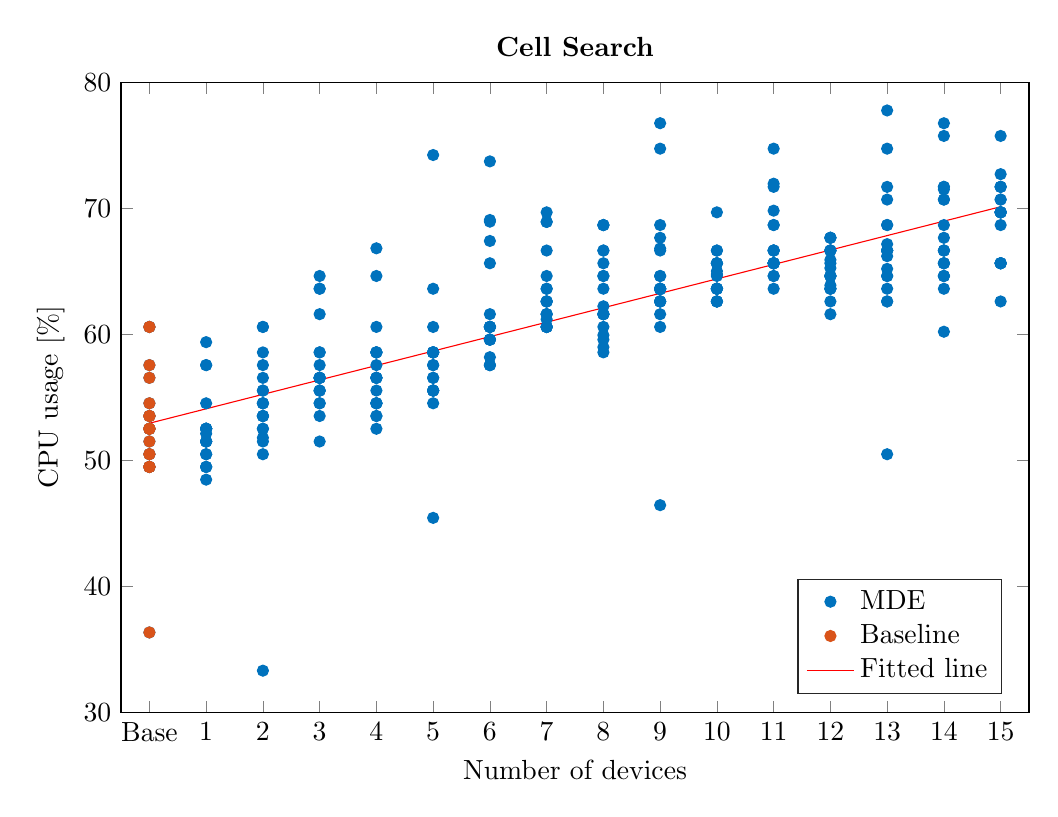
\begin{tikzpicture}

\begin{axis}[%
width=0.951\textwidth,
height=0.66\textwidth,
at={(0\textwidth,0\textwidth)},
scale only axis,
xmin=-0.5,
xmax=15.5,
xtick={0,1,2,3,4,5,6,7,8,9,10,11,12,13,14,15},
xticklabels={{Base},{1},{2},{3},{4},{5},{6},{7},{8},{9},{10},{11},{12},{13},{14},{15}},
xlabel={Number of devices},
ymin=30,
ymax=80,
ylabel={CPU usage [\%]},
axis background/.style={fill=white},
title style={font=\bfseries},
title={Cell Search},
legend style={at={(0.97,0.03)},anchor=south east,legend cell align=left,align=left,draw=white!15!black},
y tick label style={/pgf/number format/fixed}
]
\addplot [color=mycolor1,only marks,mark=*,mark options={solid}]
  table[row sep=crcr]{%
0	49.4966666666667\\
1	48.4866666666667\\
2	51.8133333333333\\
3	53.5366666666667\\
4	58.5833333333333\\
5	55.5566666666667\\
6	58.2033333333333\\
7	68.9375\\
8	61.6166666666667\\
9	62.6266666666667\\
10	63.6333333333333\\
11	65.6566666666667\\
12	64.6466666666667\\
13	77.78\\
14	64.6466666666667\\
15	71.72\\
0	36.3633333333333\\
1	51.5133333333333\\
2	57.5766666666667\\
3	55.5533333333333\\
4	53.5366666666667\\
5	58.5866666666667\\
6	57.5766666666667\\
7	61.2033333333333\\
8	59.5966666666667\\
9	63.6366666666667\\
10	64.7933333333333\\
11	68.69\\
12	64.6466666666667\\
13	66.6666666666667\\
14	66.6666666666667\\
15	69.7\\
0	57.5733333333333\\
1	52.14\\
2	55.5533333333333\\
3	56.5633333333333\\
4	55.5566666666667\\
5	58.5866666666667\\
6	69.09\\
7	68.94\\
8	64.6466666666667\\
9	76.77\\
10	65.6566666666667\\
11	65.6566666666667\\
12	62.6233333333333\\
14	75.76\\
15	65.6533333333333\\
0	53.5366666666667\\
1	50.5033333333333\\
2	53.5333333333333\\
3	56.5633333333333\\
4	64.6466666666667\\
5	58.5833333333333\\
6	61.6166666666667\\
7	66.6666666666667\\
8	66.6666666666667\\
9	66.828\\
10	62.6233333333333\\
11	66.6666666666667\\
12	65.2733333333333\\
13	71.7166666666667\\
14	71.72\\
15	62.6266666666667\\
0	52.5233333333333\\
1	51.5166666666667\\
2	58.5833333333333\\
3	56.5633333333333\\
4	54.5433333333333\\
5	45.4533333333333\\
6	59.5966666666667\\
7	60.6033333333333\\
8	66.6633333333333\\
9	63.6366666666667\\
10	65.6533333333333\\
11	71.97\\
12	66.6666666666667\\
13	66.6666666666667\\
14	70.71\\
15	72.7266666666667\\
0	54.5466666666667\\
1	57.575\\
2	60.6075\\
3	56.5633333333333\\
4	56.5633333333333\\
5	58.5866666666667\\
6	73.74\\
7	63.6333333333333\\
8	59.9533333333333\\
9	63.5766666666667\\
10	63.6366666666667\\
11	66.6666666666667\\
12	63.6366666666667\\
13	64.6433333333333\\
14	70.71\\
15	65.6566666666667\\
0	49.4966666666667\\
1	51.5133333333333\\
2	53.5366666666667\\
3	61.6166666666667\\
4	56.5666666666667\\
5	55.5566666666667\\
6	59.5933333333333\\
7	62.6233333333333\\
8	65.6566666666667\\
9	64.6466666666667\\
10	66.6633333333333\\
11	68.69\\
12	61.6133333333333\\
13	62.6266666666667\\
14	65.6566666666667\\
15	69.6966666666667\\
0	60.6033333333333\\
1	54.5433333333333\\
2	33.33\\
3	63.64\\
4	56.5633333333333\\
5	58.5833333333333\\
6	59.5966666666667\\
7	69.6966666666667\\
9	62.6233333333333\\
10	62.6233333333333\\
11	66.6666666666667\\
12	63.6333333333333\\
13	68.69\\
14	65.6533333333334\\
15	65.6566666666667\\
0	49.4966666666667\\
1	59.396\\
2	50.5033333333333\\
3	58.5866666666667\\
4	57.5733333333333\\
5	60.6033333333333\\
6	57.5733333333333\\
7	62.6266666666667\\
8	61.6133333333333\\
9	67.6766666666667\\
10	63.6366666666667\\
11	63.6333333333333\\
12	65.9233333333333\\
13	68.69\\
14	71.72\\
15	69.7\\
0	51.5166666666667\\
1	52.5233333333333\\
2	54.5433333333333\\
3	58.5866666666667\\
4	52.5233333333333\\
5	55.5533333333333\\
6	60.6066666666667\\
7	61.6166666666667\\
8	61.6166666666667\\
9	74.75\\
10	65.6533333333333\\
11	69.83\\
12	64.6433333333333\\
13	67.1733333333333\\
14	68.6866666666667\\
15	71.72\\
0	50.5066666666667\\
1	49.4966666666667\\
2	53.5333333333333\\
3	55.5533333333333\\
4	54.5466666666667\\
5	54.5466666666667\\
6	60.6033333333333\\
7	62.6266666666667\\
8	59\\
9	63.6333333333333\\
10	63.6333333333333\\
11	65.6566666666667\\
12	67.68\\
13	63.6366666666667\\
14	66.6666666666667\\
15	69.6966666666667\\
0	53.5366666666667\\
1	49.4933333333333\\
2	54.5433333333333\\
3	57.5766666666667\\
4	58.5866666666667\\
5	58.5866666666667\\
6	60.6066666666667\\
7	61.6166666666667\\
8	68.6866666666667\\
9	68.69\\
10	62.6266666666667\\
11	74.75\\
12	66.6666666666667\\
13	62.6266666666667\\
14	76.7666666666667\\
15	75.76\\
0	52.5233333333333\\
1	52.5233333333333\\
2	53.5333333333333\\
3	64.6466666666667\\
4	58.5833333333333\\
5	74.245\\
6	59.5966666666667\\
7	63.6333333333333\\
8	68.6866666666667\\
9	64.6433333333333\\
10	64.6466666666667\\
11	71.72\\
12	66.668\\
13	66.6666666666667\\
14	64.6433333333333\\
15	65.6566666666667\\
0	56.5666666666667\\
1	52.5233333333333\\
2	60.6033333333333\\
3	54.5433333333333\\
4	58.5866666666667\\
5	57.5766666666667\\
6	60.6066666666667\\
7	60.6033333333333\\
8	68.6866666666667\\
9	60.6033333333333\\
10	63.6366666666667\\
11	64.6466666666667\\
12	66.6666666666667\\
13	70.71\\
14	63.6333333333333\\
15	70.71\\
0	52.5266666666667\\
1	51.5166666666667\\
2	52.5233333333333\\
3	51.5133333333333\\
4	66.8433333333333\\
5	63.6333333333333\\
6	60.6066666666667\\
7	64.6466666666667\\
8	62.24\\
9	46.4633333333333\\
10	62.6233333333333\\
11	65.6533333333333\\
12	67.6766666666667\\
13	66.22\\
14	65.6566666666667\\
15	71.72\\
0	60.6033333333333\\
1	49.4966666666667\\
2	52.5266666666667\\
3	63.6333333333333\\
4	56.5666666666667\\
5	55.5566666666667\\
6	57.5733333333333\\
7	60.6033333333333\\
8	64.6466666666667\\
9	66.6666666666667\\
10	65.03\\
11	65.6566666666667\\
12	67.68\\
13	64.6466666666667\\
14	60.2233333333333\\
15	69.7\\
0	52.5233333333333\\
1	57.5733333333333\\
2	51.5133333333333\\
3	54.5466666666667\\
4	60.6066666666667\\
5	56.5633333333333\\
6	67.425\\
7	61.6166666666667\\
8	61.6133333333333\\
9	63.6366666666667\\
10	66.6666666666667\\
11	65.6566666666667\\
12	63.9033333333333\\
13	66.6633333333333\\
14	67.6766666666667\\
15	65.6566666666667\\
0	49.4966666666667\\
1	52.5266666666667\\
2	56.5633333333333\\
3	56.5666666666667\\
4	54.5466666666667\\
5	55.5533333333333\\
6	68.9566666666667\\
7	62.6266666666667\\
8	58.5866666666667\\
9	62.6266666666667\\
10	69.6966666666667\\
11	65.6533333333334\\
12	64.6433333333333\\
13	65.21\\
14	66.6666666666667\\
15	69.7\\
0	50.5066666666667\\
1	52.5266666666667\\
2	55.5566666666667\\
3	55.5533333333333\\
4	53.5366666666667\\
5	57.5733333333333\\
6	65.6566666666667\\
7	60.6033333333333\\
8	63.6366666666667\\
9	61.6133333333333\\
10	63.6366666666667\\
11	64.6433333333333\\
12	65.6566666666667\\
13	50.5033333333333\\
14	64.6466666666667\\
15	68.6866666666667\\
0	53.5366666666667\\
1	50.5033333333333\\
2	54.5466666666667\\
3	56.5666666666667\\
4	54.5433333333333\\
5	56.5666666666667\\
6	60.6033333333333\\
7	60.6066666666667\\
8	60.6066666666667\\
9	62.6266666666667\\
10	65.6566666666667\\
11	66.67\\
12	63.6366666666667\\
13	74.75\\
14	71.516\\
15	70.71\\
};
\addlegendentry{MDE};

\addplot [color=mycolor2,only marks,mark=*,mark options={solid}]
  table[row sep=crcr]{%
0	49.4966666666667\\
0	36.3633333333333\\
0	57.5733333333333\\
0	53.5366666666667\\
0	52.5233333333333\\
0	54.5466666666667\\
0	49.4966666666667\\
0	60.6033333333333\\
0	49.4966666666667\\
0	51.5166666666667\\
0	50.5066666666667\\
0	53.5366666666667\\
0	52.5233333333333\\
0	56.5666666666667\\
0	52.5266666666667\\
0	60.6033333333333\\
0	52.5233333333333\\
0	49.4966666666667\\
0	50.5066666666667\\
0	53.5366666666667\\
};
\addlegendentry{Baseline};

\addplot [color=red,solid]
  table[row sep=crcr]{%
0	52.9618463911013\\
0.015	52.979026850418\\
0.03	52.9962073097347\\
0.045	53.0133877690514\\
0.06	53.0305682283681\\
0.075	53.0477486876848\\
0.09	53.0649291470016\\
0.105	53.0821096063183\\
0.12	53.099290065635\\
0.135	53.1164705249517\\
0.15	53.1336509842684\\
0.165	53.1508314435851\\
0.18	53.1680119029018\\
0.195	53.1851923622185\\
0.21	53.2023728215352\\
0.225	53.2195532808519\\
0.24	53.2367337401686\\
0.255	53.2539141994853\\
0.27	53.271094658802\\
0.285	53.2882751181187\\
0.3	53.3054555774355\\
0.315	53.3226360367522\\
0.33	53.3398164960689\\
0.345	53.3569969553856\\
0.36	53.3741774147023\\
0.375	53.391357874019\\
0.39	53.4085383333357\\
0.405	53.4257187926524\\
0.42	53.4428992519691\\
0.435	53.4600797112858\\
0.45	53.4772601706025\\
0.465	53.4944406299192\\
0.48	53.5116210892359\\
0.495	53.5288015485526\\
0.51	53.5459820078694\\
0.525	53.5631624671861\\
0.54	53.5803429265028\\
0.555	53.5975233858195\\
0.57	53.6147038451362\\
0.585	53.6318843044529\\
0.6	53.6490647637696\\
0.615	53.6662452230863\\
0.63	53.683425682403\\
0.645	53.7006061417197\\
0.66	53.7177866010364\\
0.675	53.7349670603531\\
0.69	53.7521475196698\\
0.705	53.7693279789866\\
0.72	53.7865084383033\\
0.735	53.80368889762\\
0.75	53.8208693569367\\
0.765	53.8380498162534\\
0.78	53.8552302755701\\
0.795	53.8724107348868\\
0.81	53.8895911942035\\
0.825	53.9067716535202\\
0.84	53.9239521128369\\
0.855	53.9411325721536\\
0.87	53.9583130314703\\
0.885	53.975493490787\\
0.9	53.9926739501037\\
0.915	54.0098544094205\\
0.93	54.0270348687372\\
0.945	54.0442153280539\\
0.96	54.0613957873706\\
0.975	54.0785762466873\\
0.99	54.095756706004\\
1.005	54.1129371653207\\
1.02	54.1301176246374\\
1.035	54.1472980839541\\
1.05	54.1644785432708\\
1.065	54.1816590025875\\
1.08	54.1988394619042\\
1.095	54.2160199212209\\
1.11	54.2332003805376\\
1.125	54.2503808398544\\
1.14	54.2675612991711\\
1.155	54.2847417584878\\
1.17	54.3019222178045\\
1.185	54.3191026771212\\
1.2	54.3362831364379\\
1.215	54.3534635957546\\
1.23	54.3706440550713\\
1.245	54.387824514388\\
1.26	54.4050049737047\\
1.275	54.4221854330214\\
1.29	54.4393658923381\\
1.305	54.4565463516548\\
1.32	54.4737268109715\\
1.335	54.4909072702883\\
1.35	54.508087729605\\
1.365	54.5252681889217\\
1.38	54.5424486482384\\
1.395	54.5596291075551\\
1.41	54.5768095668718\\
1.425	54.5939900261885\\
1.44	54.6111704855052\\
1.455	54.6283509448219\\
1.47	54.6455314041386\\
1.485	54.6627118634553\\
1.5	54.679892322772\\
1.515	54.6970727820887\\
1.53	54.7142532414055\\
1.545	54.7314337007222\\
1.56	54.7486141600389\\
1.575	54.7657946193556\\
1.59	54.7829750786723\\
1.605	54.800155537989\\
1.62	54.8173359973057\\
1.635	54.8345164566224\\
1.65	54.8516969159391\\
1.665	54.8688773752558\\
1.68	54.8860578345725\\
1.695	54.9032382938892\\
1.71	54.9204187532059\\
1.725	54.9375992125226\\
1.74	54.9547796718394\\
1.755	54.9719601311561\\
1.77	54.9891405904728\\
1.785	55.0063210497895\\
1.8	55.0235015091062\\
1.815	55.0406819684229\\
1.83	55.0578624277396\\
1.845	55.0750428870563\\
1.86	55.092223346373\\
1.875	55.1094038056897\\
1.89	55.1265842650064\\
1.905	55.1437647243231\\
1.92	55.1609451836398\\
1.935	55.1781256429566\\
1.95	55.1953061022733\\
1.965	55.21248656159\\
1.98	55.2296670209067\\
1.995	55.2468474802234\\
2.01	55.2640279395401\\
2.025	55.2812083988568\\
2.04	55.2983888581735\\
2.055	55.3155693174902\\
2.07	55.3327497768069\\
2.085	55.3499302361236\\
2.1	55.3671106954403\\
2.115	55.384291154757\\
2.13	55.4014716140737\\
2.145	55.4186520733905\\
2.16	55.4358325327072\\
2.175	55.4530129920239\\
2.19	55.4701934513406\\
2.205	55.4873739106573\\
2.22	55.504554369974\\
2.235	55.5217348292907\\
2.25	55.5389152886074\\
2.265	55.5560957479241\\
2.28	55.5732762072408\\
2.295	55.5904566665575\\
2.31	55.6076371258742\\
2.325	55.6248175851909\\
2.34	55.6419980445077\\
2.355	55.6591785038244\\
2.37	55.6763589631411\\
2.385	55.6935394224578\\
2.4	55.7107198817745\\
2.415	55.7279003410912\\
2.43	55.7450808004079\\
2.445	55.7622612597246\\
2.46	55.7794417190413\\
2.475	55.796622178358\\
2.49	55.8138026376747\\
2.505	55.8309830969914\\
2.52	55.8481635563081\\
2.535	55.8653440156248\\
2.55	55.8825244749416\\
2.565	55.8997049342583\\
2.58	55.916885393575\\
2.595	55.9340658528917\\
2.61	55.9512463122084\\
2.625	55.9684267715251\\
2.64	55.9856072308418\\
2.655	56.0027876901585\\
2.67	56.0199681494752\\
2.685	56.0371486087919\\
2.7	56.0543290681086\\
2.715	56.0715095274253\\
2.73	56.088689986742\\
2.745	56.1058704460588\\
2.76	56.1230509053755\\
2.775	56.1402313646922\\
2.79	56.1574118240089\\
2.805	56.1745922833256\\
2.82	56.1917727426423\\
2.835	56.208953201959\\
2.85	56.2261336612757\\
2.865	56.2433141205924\\
2.88	56.2604945799091\\
2.895	56.2776750392258\\
2.91	56.2948554985425\\
2.925	56.3120359578592\\
2.94	56.3292164171759\\
2.955	56.3463968764927\\
2.97	56.3635773358094\\
2.985	56.3807577951261\\
3	56.3979382544428\\
3.015	56.4151187137595\\
3.03	56.4322991730762\\
3.045	56.4494796323929\\
3.06	56.4666600917096\\
3.075	56.4838405510263\\
3.09	56.501021010343\\
3.105	56.5182014696597\\
3.12	56.5353819289764\\
3.135	56.5525623882931\\
3.15	56.5697428476098\\
3.165	56.5869233069266\\
3.18	56.6041037662433\\
3.195	56.62128422556\\
3.21	56.6384646848767\\
3.225	56.6556451441934\\
3.24	56.6728256035101\\
3.255	56.6900060628268\\
3.27	56.7071865221435\\
3.285	56.7243669814602\\
3.3	56.7415474407769\\
3.315	56.7587279000936\\
3.33	56.7759083594103\\
3.345	56.793088818727\\
3.36	56.8102692780437\\
3.375	56.8274497373605\\
3.39	56.8446301966772\\
3.405	56.8618106559939\\
3.42	56.8789911153106\\
3.435	56.8961715746273\\
3.45	56.913352033944\\
3.465	56.9305324932607\\
3.48	56.9477129525774\\
3.495	56.9648934118941\\
3.51	56.9820738712108\\
3.525	56.9992543305275\\
3.54	57.0164347898442\\
3.555	57.0336152491609\\
3.57	57.0507957084777\\
3.585	57.0679761677944\\
3.6	57.0851566271111\\
3.615	57.1023370864278\\
3.63	57.1195175457445\\
3.645	57.1366980050612\\
3.66	57.1538784643779\\
3.675	57.1710589236946\\
3.69	57.1882393830113\\
3.705	57.205419842328\\
3.72	57.2226003016447\\
3.735	57.2397807609614\\
3.75	57.2569612202781\\
3.765	57.2741416795948\\
3.78	57.2913221389116\\
3.795	57.3085025982283\\
3.81	57.325683057545\\
3.825	57.3428635168617\\
3.84	57.3600439761784\\
3.855	57.3772244354951\\
3.87	57.3944048948118\\
3.885	57.4115853541285\\
3.9	57.4287658134452\\
3.915	57.4459462727619\\
3.93	57.4631267320786\\
3.945	57.4803071913953\\
3.96	57.497487650712\\
3.975	57.5146681100288\\
3.99	57.5318485693455\\
4.005	57.5490290286622\\
4.02	57.5662094879789\\
4.035	57.5833899472956\\
4.05	57.6005704066123\\
4.065	57.617750865929\\
4.08	57.6349313252457\\
4.095	57.6521117845624\\
4.11	57.6692922438791\\
4.125	57.6864727031958\\
4.14	57.7036531625125\\
4.155	57.7208336218292\\
4.17	57.7380140811459\\
4.185	57.7551945404627\\
4.2	57.7723749997794\\
4.215	57.7895554590961\\
4.23	57.8067359184128\\
4.245	57.8239163777295\\
4.26	57.8410968370462\\
4.275	57.8582772963629\\
4.29	57.8754577556796\\
4.305	57.8926382149963\\
4.32	57.909818674313\\
4.335	57.9269991336297\\
4.35	57.9441795929464\\
4.365	57.9613600522631\\
4.38	57.9785405115799\\
4.395	57.9957209708966\\
4.41	58.0129014302133\\
4.425	58.03008188953\\
4.44	58.0472623488467\\
4.455	58.0644428081634\\
4.47	58.0816232674801\\
4.485	58.0988037267968\\
4.5	58.1159841861135\\
4.515	58.1331646454302\\
4.53	58.1503451047469\\
4.545	58.1675255640636\\
4.56	58.1847060233803\\
4.575	58.201886482697\\
4.59	58.2190669420138\\
4.605	58.2362474013305\\
4.62	58.2534278606472\\
4.635	58.2706083199639\\
4.65	58.2877887792806\\
4.665	58.3049692385973\\
4.68	58.322149697914\\
4.695	58.3393301572307\\
4.71	58.3565106165474\\
4.725	58.3736910758641\\
4.74	58.3908715351808\\
4.755	58.4080519944975\\
4.77	58.4252324538142\\
4.785	58.442412913131\\
4.8	58.4595933724477\\
4.815	58.4767738317644\\
4.83	58.4939542910811\\
4.845	58.5111347503978\\
4.86	58.5283152097145\\
4.875	58.5454956690312\\
4.89	58.5626761283479\\
4.905	58.5798565876646\\
4.92	58.5970370469813\\
4.935	58.614217506298\\
4.95	58.6313979656147\\
4.965	58.6485784249314\\
4.98	58.6657588842481\\
4.995	58.6829393435649\\
5.01	58.7001198028816\\
5.025	58.7173002621983\\
5.04	58.734480721515\\
5.055	58.7516611808317\\
5.07	58.7688416401484\\
5.085	58.7860220994651\\
5.1	58.8032025587818\\
5.115	58.8203830180985\\
5.13	58.8375634774152\\
5.145	58.8547439367319\\
5.16	58.8719243960486\\
5.175	58.8891048553653\\
5.19	58.906285314682\\
5.205	58.9234657739988\\
5.22	58.9406462333155\\
5.235	58.9578266926322\\
5.25	58.9750071519489\\
5.265	58.9921876112656\\
5.28	59.0093680705823\\
5.295	59.026548529899\\
5.31	59.0437289892157\\
5.325	59.0609094485324\\
5.34	59.0780899078491\\
5.355	59.0952703671658\\
5.37	59.1124508264825\\
5.385	59.1296312857992\\
5.4	59.1468117451159\\
5.415	59.1639922044327\\
5.43	59.1811726637494\\
5.445	59.1983531230661\\
5.46	59.2155335823828\\
5.475	59.2327140416995\\
5.49	59.2498945010162\\
5.505	59.2670749603329\\
5.52	59.2842554196496\\
5.535	59.3014358789663\\
5.55	59.318616338283\\
5.565	59.3357967975997\\
5.58	59.3529772569164\\
5.595	59.3701577162331\\
5.61	59.3873381755499\\
5.625	59.4045186348666\\
5.64	59.4216990941833\\
5.655	59.4388795535\\
5.67	59.4560600128167\\
5.685	59.4732404721334\\
5.7	59.4904209314501\\
5.715	59.5076013907668\\
5.73	59.5247818500835\\
5.745	59.5419623094002\\
5.76	59.5591427687169\\
5.775	59.5763232280336\\
5.79	59.5935036873503\\
5.805	59.610684146667\\
5.82	59.6278646059838\\
5.835	59.6450450653005\\
5.85	59.6622255246172\\
5.865	59.6794059839339\\
5.88	59.6965864432506\\
5.895	59.7137669025673\\
5.91	59.730947361884\\
5.925	59.7481278212007\\
5.94	59.7653082805174\\
5.955	59.7824887398341\\
5.97	59.7996691991508\\
5.985	59.8168496584675\\
6	59.8340301177842\\
6.015	59.851210577101\\
6.03	59.8683910364177\\
6.045	59.8855714957344\\
6.06	59.9027519550511\\
6.075	59.9199324143678\\
6.09	59.9371128736845\\
6.105	59.9542933330012\\
6.12	59.9714737923179\\
6.135	59.9886542516346\\
6.15	60.0058347109513\\
6.165	60.023015170268\\
6.18	60.0401956295847\\
6.195	60.0573760889014\\
6.21	60.0745565482181\\
6.225	60.0917370075349\\
6.24	60.1089174668516\\
6.255	60.1260979261683\\
6.27	60.143278385485\\
6.285	60.1604588448017\\
6.3	60.1776393041184\\
6.315	60.1948197634351\\
6.33	60.2120002227518\\
6.345	60.2291806820685\\
6.36	60.2463611413852\\
6.375	60.2635416007019\\
6.39	60.2807220600186\\
6.405	60.2979025193353\\
6.42	60.3150829786521\\
6.435	60.3322634379688\\
6.45	60.3494438972855\\
6.465	60.3666243566022\\
6.48	60.3838048159189\\
6.495	60.4009852752356\\
6.51	60.4181657345523\\
6.525	60.435346193869\\
6.54	60.4525266531857\\
6.555	60.4697071125024\\
6.57	60.4868875718191\\
6.585	60.5040680311358\\
6.6	60.5212484904525\\
6.615	60.5384289497692\\
6.63	60.555609409086\\
6.645	60.5727898684027\\
6.66	60.5899703277194\\
6.675	60.6071507870361\\
6.69	60.6243312463528\\
6.705	60.6415117056695\\
6.72	60.6586921649862\\
6.735	60.6758726243029\\
6.75	60.6930530836196\\
6.765	60.7102335429363\\
6.78	60.727414002253\\
6.795	60.7445944615697\\
6.81	60.7617749208864\\
6.825	60.7789553802032\\
6.84	60.7961358395199\\
6.855	60.8133162988366\\
6.87	60.8304967581533\\
6.885	60.84767721747\\
6.9	60.8648576767867\\
6.915	60.8820381361034\\
6.93	60.8992185954201\\
6.945	60.9163990547368\\
6.96	60.9335795140535\\
6.975	60.9507599733702\\
6.99	60.9679404326869\\
7.005	60.9851208920036\\
7.02	61.0023013513203\\
7.035	61.0194818106371\\
7.05	61.0366622699538\\
7.065	61.0538427292705\\
7.08	61.0710231885872\\
7.095	61.0882036479039\\
7.11	61.1053841072206\\
7.125	61.1225645665373\\
7.14	61.139745025854\\
7.155	61.1569254851707\\
7.17	61.1741059444874\\
7.185	61.1912864038041\\
7.2	61.2084668631208\\
7.215	61.2256473224375\\
7.23	61.2428277817542\\
7.245	61.260008241071\\
7.26	61.2771887003877\\
7.275	61.2943691597044\\
7.29	61.3115496190211\\
7.305	61.3287300783378\\
7.32	61.3459105376545\\
7.335	61.3630909969712\\
7.35	61.3802714562879\\
7.365	61.3974519156046\\
7.38	61.4146323749213\\
7.395	61.431812834238\\
7.41	61.4489932935547\\
7.425	61.4661737528714\\
7.44	61.4833542121881\\
7.455	61.5005346715049\\
7.47	61.5177151308216\\
7.485	61.5348955901383\\
7.5	61.552076049455\\
7.515	61.5692565087717\\
7.53	61.5864369680884\\
7.545	61.6036174274051\\
7.56	61.6207978867218\\
7.575	61.6379783460385\\
7.59	61.6551588053552\\
7.605	61.6723392646719\\
7.62	61.6895197239886\\
7.635	61.7067001833053\\
7.65	61.723880642622\\
7.665	61.7410611019388\\
7.68	61.7582415612555\\
7.695	61.7754220205722\\
7.71	61.7926024798889\\
7.725	61.8097829392056\\
7.74	61.8269633985223\\
7.755	61.844143857839\\
7.77	61.8613243171557\\
7.785	61.8785047764724\\
7.8	61.8956852357891\\
7.815	61.9128656951058\\
7.83	61.9300461544225\\
7.845	61.9472266137392\\
7.86	61.964407073056\\
7.875	61.9815875323727\\
7.89	61.9987679916894\\
7.905	62.0159484510061\\
7.92	62.0331289103228\\
7.935	62.0503093696395\\
7.95	62.0674898289562\\
7.965	62.0846702882729\\
7.98	62.1018507475896\\
7.995	62.1190312069063\\
8.01	62.136211666223\\
8.025	62.1533921255397\\
8.04	62.1705725848564\\
8.055	62.1877530441731\\
8.07	62.2049335034899\\
8.085	62.2221139628066\\
8.1	62.2392944221233\\
8.115	62.25647488144\\
8.13	62.2736553407567\\
8.145	62.2908358000734\\
8.16	62.3080162593901\\
8.175	62.3251967187068\\
8.19	62.3423771780235\\
8.205	62.3595576373402\\
8.22	62.3767380966569\\
8.235	62.3939185559736\\
8.25	62.4110990152903\\
8.265	62.4282794746071\\
8.28	62.4454599339238\\
8.295	62.4626403932405\\
8.31	62.4798208525572\\
8.325	62.4970013118739\\
8.34	62.5141817711906\\
8.355	62.5313622305073\\
8.37	62.548542689824\\
8.385	62.5657231491407\\
8.4	62.5829036084574\\
8.415	62.6000840677741\\
8.43	62.6172645270908\\
8.445	62.6344449864075\\
8.46	62.6516254457243\\
8.475	62.668805905041\\
8.49	62.6859863643577\\
8.505	62.7031668236744\\
8.52	62.7203472829911\\
8.535	62.7375277423078\\
8.55	62.7547082016245\\
8.565	62.7718886609412\\
8.58	62.7890691202579\\
8.595	62.8062495795746\\
8.61	62.8234300388913\\
8.625	62.840610498208\\
8.64	62.8577909575247\\
8.655	62.8749714168414\\
8.67	62.8921518761582\\
8.685	62.9093323354749\\
8.7	62.9265127947916\\
8.715	62.9436932541083\\
8.73	62.960873713425\\
8.745	62.9780541727417\\
8.76	62.9952346320584\\
8.775	63.0124150913751\\
8.79	63.0295955506918\\
8.805	63.0467760100085\\
8.82	63.0639564693252\\
8.835	63.0811369286419\\
8.85	63.0983173879586\\
8.865	63.1154978472754\\
8.88	63.1326783065921\\
8.895	63.1498587659088\\
8.91	63.1670392252255\\
8.925	63.1842196845422\\
8.94	63.2014001438589\\
8.955	63.2185806031756\\
8.97	63.2357610624923\\
8.985	63.252941521809\\
9	63.2701219811257\\
9.015	63.2873024404424\\
9.03	63.3044828997591\\
9.045	63.3216633590758\\
9.06	63.3388438183925\\
9.075	63.3560242777093\\
9.09	63.373204737026\\
9.105	63.3903851963427\\
9.12	63.4075656556594\\
9.135	63.4247461149761\\
9.15	63.4419265742928\\
9.165	63.4591070336095\\
9.18	63.4762874929262\\
9.195	63.4934679522429\\
9.21	63.5106484115596\\
9.225	63.5278288708763\\
9.24	63.545009330193\\
9.255	63.5621897895097\\
9.27	63.5793702488265\\
9.285	63.5965507081432\\
9.3	63.6137311674599\\
9.315	63.6309116267766\\
9.33	63.6480920860933\\
9.345	63.66527254541\\
9.36	63.6824530047267\\
9.375	63.6996334640434\\
9.39	63.7168139233601\\
9.405	63.7339943826768\\
9.42	63.7511748419935\\
9.435	63.7683553013102\\
9.45	63.7855357606269\\
9.465	63.8027162199436\\
9.48	63.8198966792604\\
9.495	63.8370771385771\\
9.51	63.8542575978938\\
9.525	63.8714380572105\\
9.54	63.8886185165272\\
9.555	63.9057989758439\\
9.57	63.9229794351606\\
9.585	63.9401598944773\\
9.6	63.957340353794\\
9.615	63.9745208131107\\
9.63	63.9917012724274\\
9.645	64.0088817317441\\
9.66	64.0260621910608\\
9.675	64.0432426503776\\
9.69	64.0604231096943\\
9.705	64.077603569011\\
9.72	64.0947840283277\\
9.735	64.1119644876444\\
9.75	64.1291449469611\\
9.765	64.1463254062778\\
9.78	64.1635058655945\\
9.795	64.1806863249112\\
9.81	64.1978667842279\\
9.825	64.2150472435446\\
9.84	64.2322277028613\\
9.855	64.249408162178\\
9.87	64.2665886214947\\
9.885	64.2837690808115\\
9.9	64.3009495401282\\
9.915	64.3181299994449\\
9.93	64.3353104587616\\
9.945	64.3524909180783\\
9.96	64.369671377395\\
9.975	64.3868518367117\\
9.99	64.4040322960284\\
10.005	64.4212127553451\\
10.02	64.4383932146618\\
10.035	64.4555736739785\\
10.05	64.4727541332952\\
10.065	64.4899345926119\\
10.08	64.5071150519287\\
10.095	64.5242955112454\\
10.11	64.5414759705621\\
10.125	64.5586564298788\\
10.14	64.5758368891955\\
10.155	64.5930173485122\\
10.17	64.6101978078289\\
10.185	64.6273782671456\\
10.2	64.6445587264623\\
10.215	64.661739185779\\
10.23	64.6789196450957\\
10.245	64.6961001044124\\
10.26	64.7132805637291\\
10.275	64.7304610230458\\
10.29	64.7476414823626\\
10.305	64.7648219416793\\
10.32	64.782002400996\\
10.335	64.7991828603127\\
10.35	64.8163633196294\\
10.365	64.8335437789461\\
10.38	64.8507242382628\\
10.395	64.8679046975795\\
10.41	64.8850851568962\\
10.425	64.9022656162129\\
10.44	64.9194460755296\\
10.455	64.9366265348463\\
10.47	64.953806994163\\
10.485	64.9709874534797\\
10.5	64.9881679127965\\
10.515	65.0053483721132\\
10.53	65.0225288314299\\
10.545	65.0397092907466\\
10.56	65.0568897500633\\
10.575	65.07407020938\\
10.59	65.0912506686967\\
10.605	65.1084311280134\\
10.62	65.1256115873301\\
10.635	65.1427920466468\\
10.65	65.1599725059635\\
10.665	65.1771529652802\\
10.68	65.1943334245969\\
10.695	65.2115138839137\\
10.71	65.2286943432304\\
10.725	65.2458748025471\\
10.74	65.2630552618638\\
10.755	65.2802357211805\\
10.77	65.2974161804972\\
10.785	65.3145966398139\\
10.8	65.3317770991306\\
10.815	65.3489575584473\\
10.83	65.366138017764\\
10.845	65.3833184770807\\
10.86	65.4004989363974\\
10.875	65.4176793957141\\
10.89	65.4348598550308\\
10.905	65.4520403143475\\
10.92	65.4692207736643\\
10.935	65.486401232981\\
10.95	65.5035816922977\\
10.965	65.5207621516144\\
10.98	65.5379426109311\\
10.995	65.5551230702478\\
11.01	65.5723035295645\\
11.025	65.5894839888812\\
11.04	65.6066644481979\\
11.055	65.6238449075146\\
11.07	65.6410253668313\\
11.085	65.658205826148\\
11.1	65.6753862854647\\
11.115	65.6925667447815\\
11.13	65.7097472040982\\
11.145	65.7269276634149\\
11.16	65.7441081227316\\
11.175	65.7612885820483\\
11.19	65.778469041365\\
11.205	65.7956495006817\\
11.22	65.8128299599984\\
11.235	65.8300104193151\\
11.25	65.8471908786318\\
11.265	65.8643713379485\\
11.28	65.8815517972652\\
11.295	65.8987322565819\\
11.31	65.9159127158986\\
11.325	65.9330931752153\\
11.34	65.9502736345321\\
11.355	65.9674540938488\\
11.37	65.9846345531655\\
11.385	66.0018150124822\\
11.4	66.0189954717989\\
11.415	66.0361759311156\\
11.43	66.0533563904323\\
11.445	66.070536849749\\
11.46	66.0877173090657\\
11.475	66.1048977683824\\
11.49	66.1220782276991\\
11.505	66.1392586870158\\
11.52	66.1564391463325\\
11.535	66.1736196056493\\
11.55	66.190800064966\\
11.565	66.2079805242827\\
11.58	66.2251609835994\\
11.595	66.2423414429161\\
11.61	66.2595219022328\\
11.625	66.2767023615495\\
11.64	66.2938828208662\\
11.655	66.3110632801829\\
11.67	66.3282437394996\\
11.685	66.3454241988163\\
11.7	66.362604658133\\
11.715	66.3797851174497\\
11.73	66.3969655767664\\
11.745	66.4141460360832\\
11.76	66.4313264953999\\
11.775	66.4485069547166\\
11.79	66.4656874140333\\
11.805	66.48286787335\\
11.82	66.5000483326667\\
11.835	66.5172287919834\\
11.85	66.5344092513001\\
11.865	66.5515897106168\\
11.88	66.5687701699335\\
11.895	66.5859506292502\\
11.91	66.6031310885669\\
11.925	66.6203115478836\\
11.94	66.6374920072004\\
11.955	66.6546724665171\\
11.97	66.6718529258338\\
11.985	66.6890333851505\\
12	66.7062138444672\\
12.015	66.7233943037839\\
12.03	66.7405747631006\\
12.045	66.7577552224173\\
12.06	66.774935681734\\
12.075	66.7921161410507\\
12.09	66.8092966003674\\
12.105	66.8264770596841\\
12.12	66.8436575190008\\
12.135	66.8608379783175\\
12.15	66.8780184376343\\
12.165	66.895198896951\\
12.18	66.9123793562677\\
12.195	66.9295598155844\\
12.21	66.9467402749011\\
12.225	66.9639207342178\\
12.24	66.9811011935345\\
12.255	66.9982816528512\\
12.27	67.0154621121679\\
12.285	67.0326425714846\\
12.3	67.0498230308013\\
12.315	67.067003490118\\
12.33	67.0841839494347\\
12.345	67.1013644087515\\
12.36	67.1185448680682\\
12.375	67.1357253273849\\
12.39	67.1529057867016\\
12.405	67.1700862460183\\
12.42	67.187266705335\\
12.435	67.2044471646517\\
12.45	67.2216276239684\\
12.465	67.2388080832851\\
12.48	67.2559885426018\\
12.495	67.2731690019185\\
12.51	67.2903494612352\\
12.525	67.3075299205519\\
12.54	67.3247103798686\\
12.555	67.3418908391854\\
12.57	67.3590712985021\\
12.585	67.3762517578188\\
12.6	67.3934322171355\\
12.615	67.4106126764522\\
12.63	67.4277931357689\\
12.645	67.4449735950856\\
12.66	67.4621540544023\\
12.675	67.479334513719\\
12.69	67.4965149730357\\
12.705	67.5136954323524\\
12.72	67.5308758916691\\
12.735	67.5480563509858\\
12.75	67.5652368103026\\
12.765	67.5824172696193\\
12.78	67.599597728936\\
12.795	67.6167781882527\\
12.81	67.6339586475694\\
12.825	67.6511391068861\\
12.84	67.6683195662028\\
12.855	67.6855000255195\\
12.87	67.7026804848362\\
12.885	67.7198609441529\\
12.9	67.7370414034696\\
12.915	67.7542218627863\\
12.93	67.771402322103\\
12.945	67.7885827814197\\
12.96	67.8057632407365\\
12.975	67.8229437000532\\
12.99	67.8401241593699\\
13.005	67.8573046186866\\
13.02	67.8744850780033\\
13.035	67.89166553732\\
13.05	67.9088459966367\\
13.065	67.9260264559534\\
13.08	67.9432069152701\\
13.095	67.9603873745868\\
13.11	67.9775678339035\\
13.125	67.9947482932202\\
13.14	68.0119287525369\\
13.155	68.0291092118537\\
13.17	68.0462896711704\\
13.185	68.0634701304871\\
13.2	68.0806505898038\\
13.215	68.0978310491205\\
13.23	68.1150115084372\\
13.245	68.1321919677539\\
13.26	68.1493724270706\\
13.275	68.1665528863873\\
13.29	68.183733345704\\
13.305	68.2009138050207\\
13.32	68.2180942643374\\
13.335	68.2352747236541\\
13.35	68.2524551829708\\
13.365	68.2696356422876\\
13.38	68.2868161016043\\
13.395	68.303996560921\\
13.41	68.3211770202377\\
13.425	68.3383574795544\\
13.44	68.3555379388711\\
13.455	68.3727183981878\\
13.47	68.3898988575045\\
13.485	68.4070793168212\\
13.5	68.4242597761379\\
13.515	68.4414402354546\\
13.53	68.4586206947713\\
13.545	68.475801154088\\
13.56	68.4929816134048\\
13.575	68.5101620727215\\
13.59	68.5273425320382\\
13.605	68.5445229913549\\
13.62	68.5617034506716\\
13.635	68.5788839099883\\
13.65	68.596064369305\\
13.665	68.6132448286217\\
13.68	68.6304252879384\\
13.695	68.6476057472551\\
13.71	68.6647862065718\\
13.725	68.6819666658885\\
13.74	68.6991471252052\\
13.755	68.7163275845219\\
13.77	68.7335080438387\\
13.785	68.7506885031554\\
13.8	68.7678689624721\\
13.815	68.7850494217888\\
13.83	68.8022298811055\\
13.845	68.8194103404222\\
13.86	68.8365907997389\\
13.875	68.8537712590556\\
13.89	68.8709517183723\\
13.905	68.888132177689\\
13.92	68.9053126370057\\
13.935	68.9224930963224\\
13.95	68.9396735556391\\
13.965	68.9568540149559\\
13.98	68.9740344742726\\
13.995	68.9912149335893\\
14.01	69.008395392906\\
14.025	69.0255758522227\\
14.04	69.0427563115394\\
14.055	69.0599367708561\\
14.07	69.0771172301728\\
14.085	69.0942976894895\\
14.1	69.1114781488062\\
14.115	69.1286586081229\\
14.13	69.1458390674396\\
14.145	69.1630195267563\\
14.16	69.180199986073\\
14.175	69.1973804453898\\
14.19	69.2145609047065\\
14.205	69.2317413640232\\
14.22	69.2489218233399\\
14.235	69.2661022826566\\
14.25	69.2832827419733\\
14.265	69.30046320129\\
14.28	69.3176436606067\\
14.295	69.3348241199234\\
14.31	69.3520045792401\\
14.325	69.3691850385568\\
14.34	69.3863654978735\\
14.355	69.4035459571902\\
14.37	69.4207264165069\\
14.385	69.4379068758237\\
14.4	69.4550873351404\\
14.415	69.4722677944571\\
14.43	69.4894482537738\\
14.445	69.5066287130905\\
14.46	69.5238091724072\\
14.475	69.5409896317239\\
14.49	69.5581700910406\\
14.505	69.5753505503573\\
14.52	69.592531009674\\
14.535	69.6097114689907\\
14.55	69.6268919283074\\
14.565	69.6440723876241\\
14.58	69.6612528469409\\
14.595	69.6784333062576\\
14.61	69.6956137655743\\
14.625	69.712794224891\\
14.64	69.7299746842077\\
14.655	69.7471551435244\\
14.67	69.7643356028411\\
14.685	69.7815160621578\\
14.7	69.7986965214745\\
14.715	69.8158769807912\\
14.73	69.8330574401079\\
14.745	69.8502378994246\\
14.76	69.8674183587413\\
14.775	69.884598818058\\
14.79	69.9017792773747\\
14.805	69.9189597366915\\
14.82	69.9361401960082\\
14.835	69.9533206553249\\
14.85	69.9705011146416\\
14.865	69.9876815739583\\
14.88	70.004862033275\\
14.895	70.0220424925917\\
14.91	70.0392229519084\\
14.925	70.0564034112251\\
14.94	70.0735838705418\\
14.955	70.0907643298585\\
14.97	70.1079447891752\\
14.985	70.1251252484919\\
15	70.1423057078087\\
};
\addlegendentry{Fitted line};

\end{axis}
\end{tikzpicture}%}
\caption{CPU usage for the synchronization step of the MDE for different number of devices and the baseline emulator. The fitted line is a linear approximation}
\label{fig:CPU_sync}
\end{figure}

The fitted line for the CPU usage is estimated to be:
\begin{equation}
CPU_{sync} = 1.11 \cdot NoD + 53.24
\end{equation}

As seen on \autoref{fig:CPU_sync}, the average CPU usage is rising with the number of devices. This is a problem, as it will hit full usage at some point, which can effect the ability to synchronize with the cell. The synchronization is performed in a single thread, which sets the limit at 100\%, but the increase in CPU usage could be explained by the higher number of threads that is running in all the higher layer classes of each device, which means the limit could be as high as 700\%. 

\subsection{Decoding of MIB-NB}
The decoding of MIB-NB is measured from just after a cell is found until the MIB-NB has been fully decoded, the average CPU usage of this step is seen on \autoref{fig:CPU_init}. The measurements are showing only the CPU usage of the last attempt at decoding the MIB-NB if multiple attempts was made.

\begin{figure}[H]
\tikzsetnextfilename{CPU_MIB}
\centering
\resizebox{0.5\textwidth}{!}{
% This file was created by matlab2tikz.
%
%The latest updates can be retrieved from
%  http://www.mathworks.com/matlabcentral/fileexchange/22022-matlab2tikz-matlab2tikz
%where you can also make suggestions and rate matlab2tikz.
%
\definecolor{mycolor1}{rgb}{0.00000,0.44700,0.74100}%
\definecolor{mycolor2}{rgb}{0.85000,0.32500,0.09800}%
%
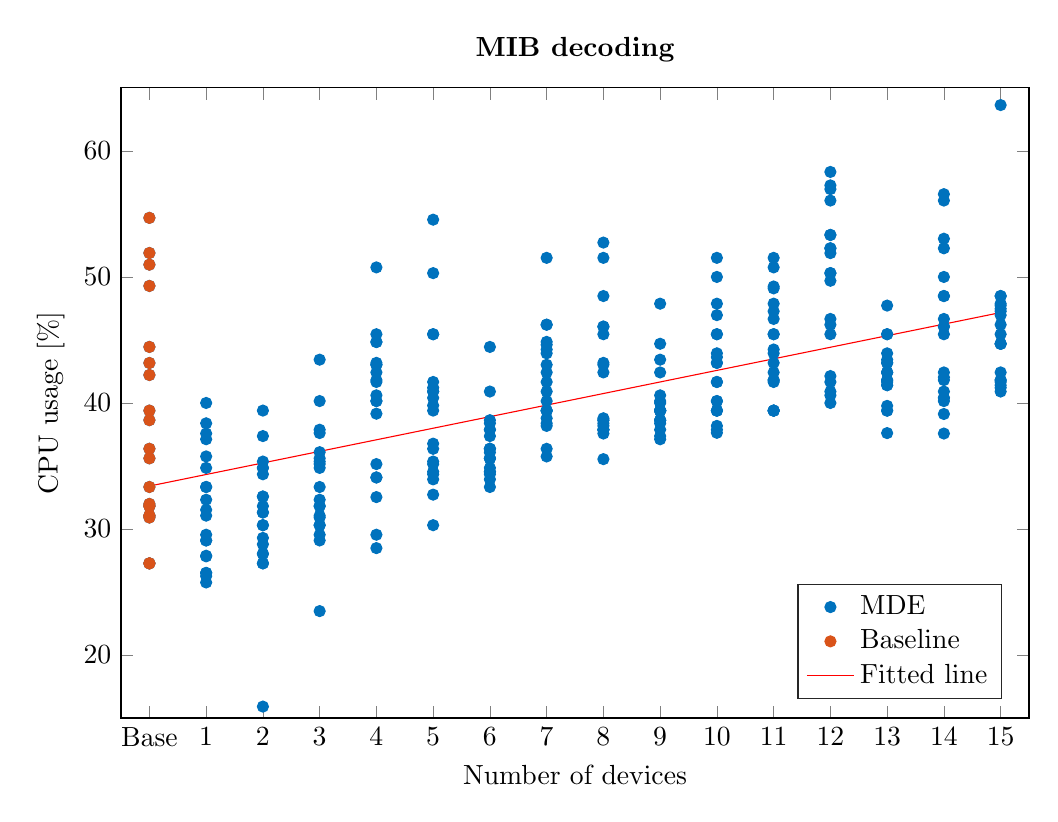
\begin{tikzpicture}

\begin{axis}[%
width=0.951\textwidth,
height=0.66\textwidth,
at={(0\textwidth,0\textwidth)},
scale only axis,
xmin=-0.5,
xmax=15.5,
xtick={0,1,2,3,4,5,6,7,8,9,10,11,12,13,14,15},
xticklabels={{Base},{1},{2},{3},{4},{5},{6},{7},{8},{9},{10},{11},{12},{13},{14},{15}},
xlabel={Number of devices},
ymin=15,
ymax=65,
ylabel={CPU usage [\%]},
axis background/.style={fill=white},
title style={font=\bfseries},
title={MIB decoding},
legend style={at={(0.97,0.03)},anchor=south east,legend cell align=left,align=left,draw=white!15!black},
y tick label style={/pgf/number format/fixed}
]
\addplot [color=mycolor1,only marks,mark=*,mark options={solid}]
  table[row sep=crcr]{%
0	31.9855555555556\\
1	37.574\\
2	39.3933333333333\\
3	29.088\\
4	35.148\\
5	35.148\\
6	36.0725\\
7	39.39\\
8	46.058\\
9	37.875\\
10	43.634\\
11	41.6625\\
12	56.0575\\
13	42.42\\
14	52.27\\
15	48.4825\\
0	31.8175\\
1	26.5125\\
2	31.815\\
3	31.0575\\
4	45.4525\\
5	41.665\\
6	36.36\\
7	46.21\\
8	37.875\\
9	38.6325\\
10	40.1475\\
11	44.24\\
12	51.888\\
13	39.39\\
14	41.814\\
15	44.695\\
0	50.9730769230769\\
1	27.876\\
2	29.29\\
3	35.6025\\
4	40.15\\
5	40.9075\\
6	37.875\\
7	43.028\\
8	46.058\\
9	39.996\\
10	39.39\\
11	49.24\\
12	57.2625\\
14	46.06\\
15	41.208\\
0	27.27\\
1	25.755\\
2	32.5725\\
3	36.0933333333333\\
4	43.028\\
5	33.936\\
6	34.542\\
7	38.784\\
8	43.028\\
9	42.42\\
10	39.39\\
11	39.39\\
12	42.1325\\
13	41.816\\
14	48.4833333333333\\
15	41.41\\
0	31.815\\
1	33.33\\
2	32.5725\\
3	30.3\\
4	41.665\\
5	34.34\\
6	36.36\\
7	43.9375\\
8	45.452\\
9	39.39\\
10	43.1775\\
11	47.27\\
12	53.33\\
13	43.43\\
14	46.058\\
15	44.6925\\
0	43.168947368421\\
1	27.8275\\
2	34.34\\
3	34.845\\
4	29.5425\\
5	39.802\\
6	35.6025\\
7	40.1475\\
8	37.875\\
9	38.6325\\
10	45.4525\\
11	43.1775\\
12	39.996\\
13	43.1775\\
14	46.664\\
15	42.4225\\
0	39.3925\\
1	29.5425\\
2	35.35\\
3	30.906\\
4	39.1475\\
5	45.4525\\
6	34.845\\
7	39.39\\
8	38.784\\
9	37.37\\
10	46.9675\\
11	45.4525\\
12	58.33\\
13	41.41\\
14	56.0575\\
15	44.695\\
0	51.89625\\
1	32.32\\
2	15.9075\\
3	31.815\\
4	32.528\\
5	36.36\\
6	35.6025\\
7	44.24\\
9	39.39\\
10	41.6625\\
11	39.39\\
12	53.33\\
13	45.4533333333333\\
14	42.42\\
15	41.814\\
0	38.635\\
1	26.26\\
2	28.0275\\
3	40.15\\
4	34.0875\\
5	36.77\\
6	34.34\\
7	41.665\\
8	37.572\\
9	40.602\\
10	43.18\\
11	39.39\\
12	50.3\\
13	45.4525\\
14	53.03\\
15	45.452\\
0	33.332\\
1	29.088\\
2	30.3\\
3	43.4333333333333\\
4	50.755\\
5	40.4\\
6	34.542\\
7	42.422\\
8	38.38\\
9	47.876\\
10	43.9375\\
11	45.452\\
12	45.4525\\
13	37.6075\\
14	48.482\\
15	47.725\\
0	54.6859090909091\\
1	38.3833333333333\\
2	28.0275\\
3	35.35\\
4	43.028\\
5	39.3925\\
6	33.936\\
7	38.38\\
8	52.724\\
9	39.39\\
10	40.1475\\
11	42.422\\
12	46.21\\
13	41.41\\
14	56.5666666666667\\
15	63.635\\
0	27.27\\
1	39.998\\
2	27.27\\
3	30.3\\
4	42.4225\\
5	40.9075\\
6	44.4433333333333\\
7	51.5125\\
8	38.6325\\
9	43.4333333333333\\
10	49.9975\\
11	46.666\\
12	52.27\\
13	42.42\\
14	49.9975\\
15	46.9675\\
0	31.0575\\
1	29.088\\
2	37.37\\
3	37.875\\
4	34.0875\\
5	34.542\\
6	36.36\\
7	39.39\\
8	37.875\\
9	44.695\\
10	39.39\\
11	39.39\\
12	40.905\\
13	42.4225\\
14	40.4\\
15	41.814\\
0	44.445\\
1	31.512\\
2	34.845\\
3	32.32\\
4	40.15\\
5	41.21\\
6	37.875\\
7	35.754\\
8	48.4825\\
9	37.1175\\
10	37.875\\
11	51.5125\\
12	49.694\\
13	47.725\\
14	37.572\\
15	48.4825\\
0	36.3625\\
1	37.12\\
2	27.27\\
3	35.15\\
4	44.8275\\
5	30.3\\
6	38.3833333333333\\
7	44.616\\
8	38.178\\
9	38.38\\
10	38.178\\
11	41.814\\
12	56.966\\
13	43.1775\\
14	40.4\\
15	47.272\\
0	42.2178947368421\\
1	35.756\\
2	34.845\\
3	33.33\\
4	43.18\\
5	45.4525\\
6	33.33\\
7	36.36\\
8	42.4225\\
9	40.1475\\
10	37.63\\
11	50.755\\
12	46.664\\
13	41.665\\
14	42.0366666666667\\
15	47.878\\
0	31.0575\\
1	31.0575\\
2	28.785\\
3	29.5425\\
4	41.816\\
5	50.3\\
6	37.37\\
7	46.21\\
8	35.54\\
9	38.6325\\
10	45.4525\\
11	49.09\\
12	41.6625\\
13	43.935\\
14	45.45\\
15	40.905\\
0	35.605\\
1	33.332\\
2	31.31\\
3	23.4825\\
4	40.604\\
5	54.5425\\
6	35.6025\\
7	40.9075\\
8	51.5125\\
9	39.39\\
10	47.876\\
11	43.9375\\
12	40.602\\
13	39.766\\
14	39.1225\\
15	47.4733333333333\\
0	30.908\\
1	26.5125\\
2	30.3\\
3	31.815\\
4	44.846\\
5	35.35\\
6	40.905\\
7	38.178\\
8	43.18\\
9	39.39\\
10	41.665\\
11	41.814\\
12	50.3\\
13	39.39\\
14	40.1475\\
15	41.6625\\
0	49.2844736842105\\
1	34.845\\
2	31.31\\
3	37.61\\
4	28.482\\
5	32.724\\
6	38.6325\\
7	44.846\\
8	38.6325\\
9	39.39\\
10	51.5133333333333\\
11	47.878\\
12	52.27\\
13	41.814\\
14	40.905\\
15	46.21\\
};
\addlegendentry{MDE};

\addplot [color=mycolor2,only marks,mark=*,mark options={solid}]
  table[row sep=crcr]{%
0	31.9855555555556\\
0	31.8175\\
0	50.9730769230769\\
0	27.27\\
0	31.815\\
0	43.168947368421\\
0	39.3925\\
0	51.89625\\
0	38.635\\
0	33.332\\
0	54.6859090909091\\
0	27.27\\
0	31.0575\\
0	44.445\\
0	36.3625\\
0	42.2178947368421\\
0	31.0575\\
0	35.605\\
0	30.908\\
0	49.2844736842105\\
};
\addlegendentry{Baseline};

\addplot [color=red,solid]
  table[row sep=crcr]{%
0	33.4040515760645\\
0.015	33.4178189165826\\
0.03	33.4315862571007\\
0.045	33.4453535976188\\
0.06	33.4591209381369\\
0.075	33.472888278655\\
0.09	33.4866556191731\\
0.105	33.5004229596912\\
0.12	33.5141903002093\\
0.135	33.5279576407274\\
0.15	33.5417249812455\\
0.165	33.5554923217636\\
0.18	33.5692596622817\\
0.195	33.5830270027998\\
0.21	33.5967943433179\\
0.225	33.610561683836\\
0.24	33.6243290243541\\
0.255	33.6380963648722\\
0.27	33.6518637053903\\
0.285	33.6656310459084\\
0.3	33.6793983864265\\
0.315	33.6931657269446\\
0.33	33.7069330674627\\
0.345	33.7207004079808\\
0.36	33.7344677484989\\
0.375	33.748235089017\\
0.39	33.7620024295351\\
0.405	33.7757697700532\\
0.42	33.7895371105713\\
0.435	33.8033044510894\\
0.45	33.8170717916075\\
0.465	33.8308391321256\\
0.48	33.8446064726437\\
0.495	33.8583738131618\\
0.51	33.8721411536799\\
0.525	33.885908494198\\
0.54	33.8996758347161\\
0.555	33.9134431752342\\
0.57	33.9272105157523\\
0.585	33.9409778562704\\
0.6	33.9547451967885\\
0.615	33.9685125373066\\
0.63	33.9822798778247\\
0.645	33.9960472183428\\
0.66	34.0098145588609\\
0.675	34.023581899379\\
0.69	34.0373492398971\\
0.705	34.0511165804152\\
0.72	34.0648839209333\\
0.735	34.0786512614514\\
0.75	34.0924186019695\\
0.765	34.1061859424876\\
0.78	34.1199532830057\\
0.795	34.1337206235238\\
0.81	34.1474879640419\\
0.825	34.16125530456\\
0.84	34.1750226450781\\
0.855	34.1887899855962\\
0.87	34.2025573261143\\
0.885	34.2163246666324\\
0.9	34.2300920071505\\
0.915	34.2438593476686\\
0.93	34.2576266881867\\
0.945	34.2713940287048\\
0.96	34.2851613692229\\
0.975	34.298928709741\\
0.99	34.3126960502591\\
1.005	34.3264633907772\\
1.02	34.3402307312953\\
1.035	34.3539980718134\\
1.05	34.3677654123315\\
1.065	34.3815327528496\\
1.08	34.3953000933677\\
1.095	34.4090674338858\\
1.11	34.4228347744039\\
1.125	34.436602114922\\
1.14	34.4503694554401\\
1.155	34.4641367959582\\
1.17	34.4779041364762\\
1.185	34.4916714769943\\
1.2	34.5054388175124\\
1.215	34.5192061580305\\
1.23	34.5329734985487\\
1.245	34.5467408390667\\
1.26	34.5605081795848\\
1.275	34.5742755201029\\
1.29	34.588042860621\\
1.305	34.6018102011391\\
1.32	34.6155775416572\\
1.335	34.6293448821753\\
1.35	34.6431122226934\\
1.365	34.6568795632115\\
1.38	34.6706469037296\\
1.395	34.6844142442477\\
1.41	34.6981815847658\\
1.425	34.7119489252839\\
1.44	34.725716265802\\
1.455	34.7394836063201\\
1.47	34.7532509468382\\
1.485	34.7670182873563\\
1.5	34.7807856278744\\
1.515	34.7945529683925\\
1.53	34.8083203089106\\
1.545	34.8220876494287\\
1.56	34.8358549899468\\
1.575	34.8496223304649\\
1.59	34.863389670983\\
1.605	34.8771570115011\\
1.62	34.8909243520192\\
1.635	34.9046916925373\\
1.65	34.9184590330554\\
1.665	34.9322263735735\\
1.68	34.9459937140916\\
1.695	34.9597610546097\\
1.71	34.9735283951278\\
1.725	34.9872957356459\\
1.74	35.001063076164\\
1.755	35.0148304166821\\
1.77	35.0285977572002\\
1.785	35.0423650977183\\
1.8	35.0561324382364\\
1.815	35.0698997787545\\
1.83	35.0836671192726\\
1.845	35.0974344597907\\
1.86	35.1112018003088\\
1.875	35.1249691408269\\
1.89	35.138736481345\\
1.905	35.1525038218631\\
1.92	35.1662711623812\\
1.935	35.1800385028993\\
1.95	35.1938058434174\\
1.965	35.2075731839355\\
1.98	35.2213405244536\\
1.995	35.2351078649717\\
2.01	35.2488752054898\\
2.025	35.2626425460079\\
2.04	35.276409886526\\
2.055	35.2901772270441\\
2.07	35.3039445675622\\
2.085	35.3177119080803\\
2.1	35.3314792485984\\
2.115	35.3452465891165\\
2.13	35.3590139296346\\
2.145	35.3727812701527\\
2.16	35.3865486106708\\
2.175	35.4003159511889\\
2.19	35.414083291707\\
2.205	35.4278506322251\\
2.22	35.4416179727432\\
2.235	35.4553853132613\\
2.25	35.4691526537794\\
2.265	35.4829199942975\\
2.28	35.4966873348156\\
2.295	35.5104546753337\\
2.31	35.5242220158518\\
2.325	35.5379893563699\\
2.34	35.551756696888\\
2.355	35.5655240374061\\
2.37	35.5792913779242\\
2.385	35.5930587184423\\
2.4	35.6068260589604\\
2.415	35.6205933994785\\
2.43	35.6343607399966\\
2.445	35.6481280805147\\
2.46	35.6618954210328\\
2.475	35.6756627615509\\
2.49	35.689430102069\\
2.505	35.7031974425871\\
2.52	35.7169647831052\\
2.535	35.7307321236233\\
2.55	35.7444994641414\\
2.565	35.7582668046595\\
2.58	35.7720341451776\\
2.595	35.7858014856957\\
2.61	35.7995688262138\\
2.625	35.8133361667319\\
2.64	35.82710350725\\
2.655	35.840870847768\\
2.67	35.8546381882861\\
2.685	35.8684055288042\\
2.7	35.8821728693223\\
2.715	35.8959402098404\\
2.73	35.9097075503585\\
2.745	35.9234748908766\\
2.76	35.9372422313947\\
2.775	35.9510095719128\\
2.79	35.9647769124309\\
2.805	35.978544252949\\
2.82	35.9923115934671\\
2.835	36.0060789339852\\
2.85	36.0198462745033\\
2.865	36.0336136150214\\
2.88	36.0473809555395\\
2.895	36.0611482960576\\
2.91	36.0749156365757\\
2.925	36.0886829770938\\
2.94	36.1024503176119\\
2.955	36.11621765813\\
2.97	36.1299849986481\\
2.985	36.1437523391662\\
3	36.1575196796843\\
3.015	36.1712870202024\\
3.03	36.1850543607205\\
3.045	36.1988217012386\\
3.06	36.2125890417567\\
3.075	36.2263563822748\\
3.09	36.2401237227929\\
3.105	36.253891063311\\
3.12	36.2676584038291\\
3.135	36.2814257443472\\
3.15	36.2951930848653\\
3.165	36.3089604253834\\
3.18	36.3227277659015\\
3.195	36.3364951064196\\
3.21	36.3502624469377\\
3.225	36.3640297874558\\
3.24	36.3777971279739\\
3.255	36.391564468492\\
3.27	36.4053318090101\\
3.285	36.4190991495282\\
3.3	36.4328664900463\\
3.315	36.4466338305644\\
3.33	36.4604011710825\\
3.345	36.4741685116006\\
3.36	36.4879358521187\\
3.375	36.5017031926368\\
3.39	36.5154705331549\\
3.405	36.529237873673\\
3.42	36.5430052141911\\
3.435	36.5567725547092\\
3.45	36.5705398952273\\
3.465	36.5843072357454\\
3.48	36.5980745762635\\
3.495	36.6118419167816\\
3.51	36.6256092572997\\
3.525	36.6393765978178\\
3.54	36.6531439383359\\
3.555	36.666911278854\\
3.57	36.6806786193721\\
3.585	36.6944459598902\\
3.6	36.7082133004083\\
3.615	36.7219806409264\\
3.63	36.7357479814445\\
3.645	36.7495153219626\\
3.66	36.7632826624807\\
3.675	36.7770500029988\\
3.69	36.7908173435169\\
3.705	36.804584684035\\
3.72	36.8183520245531\\
3.735	36.8321193650712\\
3.75	36.8458867055893\\
3.765	36.8596540461074\\
3.78	36.8734213866255\\
3.795	36.8871887271436\\
3.81	36.9009560676617\\
3.825	36.9147234081798\\
3.84	36.9284907486979\\
3.855	36.942258089216\\
3.87	36.9560254297341\\
3.885	36.9697927702522\\
3.9	36.9835601107703\\
3.915	36.9973274512884\\
3.93	37.0110947918065\\
3.945	37.0248621323246\\
3.96	37.0386294728427\\
3.975	37.0523968133608\\
3.99	37.0661641538789\\
4.005	37.079931494397\\
4.02	37.0936988349151\\
4.035	37.1074661754332\\
4.05	37.1212335159513\\
4.065	37.1350008564694\\
4.08	37.1487681969874\\
4.095	37.1625355375055\\
4.11	37.1763028780236\\
4.125	37.1900702185417\\
4.14	37.2038375590598\\
4.155	37.2176048995779\\
4.17	37.231372240096\\
4.185	37.2451395806141\\
4.2	37.2589069211322\\
4.215	37.2726742616503\\
4.23	37.2864416021684\\
4.245	37.3002089426865\\
4.26	37.3139762832046\\
4.275	37.3277436237227\\
4.29	37.3415109642408\\
4.305	37.3552783047589\\
4.32	37.369045645277\\
4.335	37.3828129857951\\
4.35	37.3965803263132\\
4.365	37.4103476668313\\
4.38	37.4241150073494\\
4.395	37.4378823478675\\
4.41	37.4516496883856\\
4.425	37.4654170289037\\
4.44	37.4791843694218\\
4.455	37.4929517099399\\
4.47	37.506719050458\\
4.485	37.5204863909761\\
4.5	37.5342537314942\\
4.515	37.5480210720123\\
4.53	37.5617884125304\\
4.545	37.5755557530485\\
4.56	37.5893230935666\\
4.575	37.6030904340847\\
4.59	37.6168577746028\\
4.605	37.6306251151209\\
4.62	37.644392455639\\
4.635	37.6581597961571\\
4.65	37.6719271366752\\
4.665	37.6856944771933\\
4.68	37.6994618177114\\
4.695	37.7132291582295\\
4.71	37.7269964987476\\
4.725	37.7407638392657\\
4.74	37.7545311797838\\
4.755	37.7682985203019\\
4.77	37.78206586082\\
4.785	37.7958332013381\\
4.8	37.8096005418562\\
4.815	37.8233678823743\\
4.83	37.8371352228924\\
4.845	37.8509025634105\\
4.86	37.8646699039286\\
4.875	37.8784372444467\\
4.89	37.8922045849648\\
4.905	37.9059719254829\\
4.92	37.919739266001\\
4.935	37.9335066065191\\
4.95	37.9472739470372\\
4.965	37.9610412875553\\
4.98	37.9748086280734\\
4.995	37.9885759685915\\
5.01	38.0023433091096\\
5.025	38.0161106496277\\
5.04	38.0298779901458\\
5.055	38.0436453306639\\
5.07	38.057412671182\\
5.085	38.0711800117001\\
5.1	38.0849473522182\\
5.115	38.0987146927363\\
5.13	38.1124820332544\\
5.145	38.1262493737725\\
5.16	38.1400167142906\\
5.175	38.1537840548087\\
5.19	38.1675513953268\\
5.205	38.1813187358449\\
5.22	38.195086076363\\
5.235	38.2088534168811\\
5.25	38.2226207573992\\
5.265	38.2363880979173\\
5.28	38.2501554384354\\
5.295	38.2639227789535\\
5.31	38.2776901194716\\
5.325	38.2914574599897\\
5.34	38.3052248005078\\
5.355	38.3189921410259\\
5.37	38.332759481544\\
5.385	38.3465268220621\\
5.4	38.3602941625802\\
5.415	38.3740615030983\\
5.43	38.3878288436164\\
5.445	38.4015961841345\\
5.46	38.4153635246526\\
5.475	38.4291308651707\\
5.49	38.4428982056887\\
5.505	38.4566655462069\\
5.52	38.470432886725\\
5.535	38.4842002272431\\
5.55	38.4979675677612\\
5.565	38.5117349082792\\
5.58	38.5255022487973\\
5.595	38.5392695893154\\
5.61	38.5530369298335\\
5.625	38.5668042703516\\
5.64	38.5805716108697\\
5.655	38.5943389513878\\
5.67	38.6081062919059\\
5.685	38.621873632424\\
5.7	38.6356409729421\\
5.715	38.6494083134602\\
5.73	38.6631756539783\\
5.745	38.6769429944964\\
5.76	38.6907103350145\\
5.775	38.7044776755326\\
5.79	38.7182450160507\\
5.805	38.7320123565688\\
5.82	38.7457796970869\\
5.835	38.759547037605\\
5.85	38.7733143781231\\
5.865	38.7870817186412\\
5.88	38.8008490591593\\
5.895	38.8146163996774\\
5.91	38.8283837401955\\
5.925	38.8421510807136\\
5.94	38.8559184212317\\
5.955	38.8696857617498\\
5.97	38.8834531022679\\
5.985	38.897220442786\\
6	38.9109877833041\\
6.015	38.9247551238222\\
6.03	38.9385224643403\\
6.045	38.9522898048584\\
6.06	38.9660571453765\\
6.075	38.9798244858946\\
6.09	38.9935918264127\\
6.105	39.0073591669308\\
6.12	39.0211265074489\\
6.135	39.034893847967\\
6.15	39.0486611884851\\
6.165	39.0624285290032\\
6.18	39.0761958695213\\
6.195	39.0899632100394\\
6.21	39.1037305505575\\
6.225	39.1174978910756\\
6.24	39.1312652315937\\
6.255	39.1450325721118\\
6.27	39.1587999126299\\
6.285	39.172567253148\\
6.3	39.1863345936661\\
6.315	39.2001019341842\\
6.33	39.2138692747023\\
6.345	39.2276366152204\\
6.36	39.2414039557385\\
6.375	39.2551712962566\\
6.39	39.2689386367747\\
6.405	39.2827059772928\\
6.42	39.2964733178109\\
6.435	39.310240658329\\
6.45	39.3240079988471\\
6.465	39.3377753393652\\
6.48	39.3515426798833\\
6.495	39.3653100204014\\
6.51	39.3790773609195\\
6.525	39.3928447014376\\
6.54	39.4066120419557\\
6.555	39.4203793824738\\
6.57	39.4341467229919\\
6.585	39.44791406351\\
6.6	39.4616814040281\\
6.615	39.4754487445462\\
6.63	39.4892160850643\\
6.645	39.5029834255824\\
6.66	39.5167507661005\\
6.675	39.5305181066186\\
6.69	39.5442854471367\\
6.705	39.5580527876548\\
6.72	39.5718201281729\\
6.735	39.585587468691\\
6.75	39.5993548092091\\
6.765	39.6131221497272\\
6.78	39.6268894902453\\
6.795	39.6406568307634\\
6.81	39.6544241712815\\
6.825	39.6681915117996\\
6.84	39.6819588523177\\
6.855	39.6957261928358\\
6.87	39.7094935333539\\
6.885	39.723260873872\\
6.9	39.7370282143901\\
6.915	39.7507955549082\\
6.93	39.7645628954263\\
6.945	39.7783302359444\\
6.96	39.7920975764625\\
6.975	39.8058649169806\\
6.99	39.8196322574986\\
7.005	39.8333995980167\\
7.02	39.8471669385348\\
7.035	39.8609342790529\\
7.05	39.874701619571\\
7.065	39.8884689600891\\
7.08	39.9022363006072\\
7.095	39.9160036411253\\
7.11	39.9297709816434\\
7.125	39.9435383221615\\
7.14	39.9573056626796\\
7.155	39.9710730031977\\
7.17	39.9848403437158\\
7.185	39.9986076842339\\
7.2	40.012375024752\\
7.215	40.0261423652701\\
7.23	40.0399097057882\\
7.245	40.0536770463063\\
7.26	40.0674443868244\\
7.275	40.0812117273425\\
7.29	40.0949790678606\\
7.305	40.1087464083787\\
7.32	40.1225137488968\\
7.335	40.1362810894149\\
7.35	40.150048429933\\
7.365	40.1638157704511\\
7.38	40.1775831109692\\
7.395	40.1913504514873\\
7.41	40.2051177920054\\
7.425	40.2188851325235\\
7.44	40.2326524730416\\
7.455	40.2464198135597\\
7.47	40.2601871540778\\
7.485	40.2739544945959\\
7.5	40.287721835114\\
7.515	40.3014891756321\\
7.53	40.3152565161502\\
7.545	40.3290238566683\\
7.56	40.3427911971864\\
7.575	40.3565585377045\\
7.59	40.3703258782226\\
7.605	40.3840932187407\\
7.62	40.3978605592588\\
7.635	40.4116278997769\\
7.65	40.425395240295\\
7.665	40.4391625808131\\
7.68	40.4529299213312\\
7.695	40.4666972618493\\
7.71	40.4804646023674\\
7.725	40.4942319428855\\
7.74	40.5079992834036\\
7.755	40.5217666239217\\
7.77	40.5355339644398\\
7.785	40.5493013049579\\
7.8	40.563068645476\\
7.815	40.5768359859941\\
7.83	40.5906033265122\\
7.845	40.6043706670303\\
7.86	40.6181380075484\\
7.875	40.6319053480665\\
7.89	40.6456726885846\\
7.905	40.6594400291027\\
7.92	40.6732073696208\\
7.935	40.6869747101389\\
7.95	40.700742050657\\
7.965	40.7145093911751\\
7.98	40.7282767316932\\
7.995	40.7420440722113\\
8.01	40.7558114127294\\
8.025	40.7695787532475\\
8.04	40.7833460937656\\
8.055	40.7971134342837\\
8.07	40.8108807748018\\
8.085	40.8246481153199\\
8.1	40.838415455838\\
8.115	40.8521827963561\\
8.13	40.8659501368742\\
8.145	40.8797174773923\\
8.16	40.8934848179104\\
8.175	40.9072521584285\\
8.19	40.9210194989466\\
8.205	40.9347868394647\\
8.22	40.9485541799828\\
8.235	40.9623215205009\\
8.25	40.976088861019\\
8.265	40.9898562015371\\
8.28	41.0036235420552\\
8.295	41.0173908825733\\
8.31	41.0311582230914\\
8.325	41.0449255636095\\
8.34	41.0586929041276\\
8.355	41.0724602446457\\
8.37	41.0862275851638\\
8.385	41.0999949256819\\
8.4	41.1137622662\\
8.415	41.127529606718\\
8.43	41.1412969472362\\
8.445	41.1550642877543\\
8.46	41.1688316282723\\
8.475	41.1825989687904\\
8.49	41.1963663093085\\
8.505	41.2101336498266\\
8.52	41.2239009903447\\
8.535	41.2376683308628\\
8.55	41.2514356713809\\
8.565	41.265203011899\\
8.58	41.2789703524171\\
8.595	41.2927376929352\\
8.61	41.3065050334533\\
8.625	41.3202723739714\\
8.64	41.3340397144895\\
8.655	41.3478070550076\\
8.67	41.3615743955257\\
8.685	41.3753417360438\\
8.7	41.3891090765619\\
8.715	41.40287641708\\
8.73	41.4166437575981\\
8.745	41.4304110981162\\
8.76	41.4441784386343\\
8.775	41.4579457791524\\
8.79	41.4717131196705\\
8.805	41.4854804601886\\
8.82	41.4992478007067\\
8.835	41.5130151412248\\
8.85	41.5267824817429\\
8.865	41.540549822261\\
8.88	41.5543171627791\\
8.895	41.5680845032972\\
8.91	41.5818518438153\\
8.925	41.5956191843334\\
8.94	41.6093865248515\\
8.955	41.6231538653696\\
8.97	41.6369212058877\\
8.985	41.6506885464058\\
9	41.6644558869239\\
9.015	41.678223227442\\
9.03	41.6919905679601\\
9.045	41.7057579084782\\
9.06	41.7195252489963\\
9.075	41.7332925895144\\
9.09	41.7470599300325\\
9.105	41.7608272705506\\
9.12	41.7745946110687\\
9.135	41.7883619515868\\
9.15	41.8021292921049\\
9.165	41.815896632623\\
9.18	41.8296639731411\\
9.195	41.8434313136592\\
9.21	41.8571986541773\\
9.225	41.8709659946954\\
9.24	41.8847333352135\\
9.255	41.8985006757316\\
9.27	41.9122680162497\\
9.285	41.9260353567678\\
9.3	41.9398026972859\\
9.315	41.953570037804\\
9.33	41.9673373783221\\
9.345	41.9811047188402\\
9.36	41.9948720593583\\
9.375	42.0086393998764\\
9.39	42.0224067403945\\
9.405	42.0361740809126\\
9.42	42.0499414214307\\
9.435	42.0637087619488\\
9.45	42.0774761024669\\
9.465	42.091243442985\\
9.48	42.1050107835031\\
9.495	42.1187781240212\\
9.51	42.1325454645393\\
9.525	42.1463128050574\\
9.54	42.1600801455755\\
9.555	42.1738474860936\\
9.57	42.1876148266117\\
9.585	42.2013821671298\\
9.6	42.2151495076479\\
9.615	42.228916848166\\
9.63	42.2426841886841\\
9.645	42.2564515292022\\
9.66	42.2702188697203\\
9.675	42.2839862102384\\
9.69	42.2977535507565\\
9.705	42.3115208912746\\
9.72	42.3252882317927\\
9.735	42.3390555723108\\
9.75	42.3528229128289\\
9.765	42.366590253347\\
9.78	42.3803575938651\\
9.795	42.3941249343832\\
9.81	42.4078922749013\\
9.825	42.4216596154194\\
9.84	42.4354269559375\\
9.855	42.4491942964556\\
9.87	42.4629616369736\\
9.885	42.4767289774917\\
9.9	42.4904963180098\\
9.915	42.5042636585279\\
9.93	42.518030999046\\
9.945	42.5317983395641\\
9.96	42.5455656800822\\
9.975	42.5593330206003\\
9.99	42.5731003611184\\
10.005	42.5868677016365\\
10.02	42.6006350421546\\
10.035	42.6144023826727\\
10.05	42.6281697231908\\
10.065	42.6419370637089\\
10.08	42.655704404227\\
10.095	42.6694717447451\\
10.11	42.6832390852632\\
10.125	42.6970064257813\\
10.14	42.7107737662994\\
10.155	42.7245411068175\\
10.17	42.7383084473356\\
10.185	42.7520757878537\\
10.2	42.7658431283718\\
10.215	42.7796104688899\\
10.23	42.793377809408\\
10.245	42.8071451499261\\
10.26	42.8209124904442\\
10.275	42.8346798309623\\
10.29	42.8484471714804\\
10.305	42.8622145119985\\
10.32	42.8759818525166\\
10.335	42.8897491930347\\
10.35	42.9035165335528\\
10.365	42.9172838740709\\
10.38	42.931051214589\\
10.395	42.9448185551071\\
10.41	42.9585858956252\\
10.425	42.9723532361433\\
10.44	42.9861205766614\\
10.455	42.9998879171795\\
10.47	43.0136552576976\\
10.485	43.0274225982157\\
10.5	43.0411899387338\\
10.515	43.0549572792519\\
10.53	43.06872461977\\
10.545	43.0824919602881\\
10.56	43.0962593008062\\
10.575	43.1100266413243\\
10.59	43.1237939818424\\
10.605	43.1375613223605\\
10.62	43.1513286628786\\
10.635	43.1650960033967\\
10.65	43.1788633439148\\
10.665	43.1926306844329\\
10.68	43.206398024951\\
10.695	43.2201653654691\\
10.71	43.2339327059872\\
10.725	43.2477000465053\\
10.74	43.2614673870234\\
10.755	43.2752347275415\\
10.77	43.2890020680596\\
10.785	43.3027694085777\\
10.8	43.3165367490958\\
10.815	43.3303040896139\\
10.83	43.344071430132\\
10.845	43.3578387706501\\
10.86	43.3716061111682\\
10.875	43.3853734516863\\
10.89	43.3991407922044\\
10.905	43.4129081327225\\
10.92	43.4266754732406\\
10.935	43.4404428137587\\
10.95	43.4542101542768\\
10.965	43.4679774947949\\
10.98	43.481744835313\\
10.995	43.4955121758311\\
11.01	43.5092795163492\\
11.025	43.5230468568673\\
11.04	43.5368141973854\\
11.055	43.5505815379035\\
11.07	43.5643488784216\\
11.085	43.5781162189397\\
11.1	43.5918835594578\\
11.115	43.6056508999759\\
11.13	43.619418240494\\
11.145	43.6331855810121\\
11.16	43.6469529215302\\
11.175	43.6607202620483\\
11.19	43.6744876025664\\
11.205	43.6882549430845\\
11.22	43.7020222836026\\
11.235	43.7157896241207\\
11.25	43.7295569646388\\
11.265	43.7433243051569\\
11.28	43.757091645675\\
11.295	43.770858986193\\
11.31	43.7846263267111\\
11.325	43.7983936672292\\
11.34	43.8121610077473\\
11.355	43.8259283482655\\
11.37	43.8396956887836\\
11.385	43.8534630293016\\
11.4	43.8672303698197\\
11.415	43.8809977103378\\
11.43	43.8947650508559\\
11.445	43.908532391374\\
11.46	43.9222997318921\\
11.475	43.9360670724102\\
11.49	43.9498344129283\\
11.505	43.9636017534464\\
11.52	43.9773690939645\\
11.535	43.9911364344826\\
11.55	44.0049037750007\\
11.565	44.0186711155188\\
11.58	44.0324384560369\\
11.595	44.046205796555\\
11.61	44.0599731370731\\
11.625	44.0737404775912\\
11.64	44.0875078181093\\
11.655	44.1012751586274\\
11.67	44.1150424991455\\
11.685	44.1288098396636\\
11.7	44.1425771801817\\
11.715	44.1563445206998\\
11.73	44.1701118612179\\
11.745	44.183879201736\\
11.76	44.1976465422541\\
11.775	44.2114138827722\\
11.79	44.2251812232903\\
11.805	44.2389485638084\\
11.82	44.2527159043265\\
11.835	44.2664832448446\\
11.85	44.2802505853627\\
11.865	44.2940179258808\\
11.88	44.3077852663989\\
11.895	44.321552606917\\
11.91	44.3353199474351\\
11.925	44.3490872879532\\
11.94	44.3628546284713\\
11.955	44.3766219689894\\
11.97	44.3903893095075\\
11.985	44.4041566500256\\
12	44.4179239905437\\
12.015	44.4316913310618\\
12.03	44.4454586715799\\
12.045	44.459226012098\\
12.06	44.4729933526161\\
12.075	44.4867606931342\\
12.09	44.5005280336523\\
12.105	44.5142953741704\\
12.12	44.5280627146885\\
12.135	44.5418300552066\\
12.15	44.5555973957247\\
12.165	44.5693647362428\\
12.18	44.5831320767609\\
12.195	44.596899417279\\
12.21	44.6106667577971\\
12.225	44.6244340983152\\
12.24	44.6382014388333\\
12.255	44.6519687793514\\
12.27	44.6657361198695\\
12.285	44.6795034603876\\
12.3	44.6932708009057\\
12.315	44.7070381414238\\
12.33	44.7208054819419\\
12.345	44.73457282246\\
12.36	44.7483401629781\\
12.375	44.7621075034962\\
12.39	44.7758748440143\\
12.405	44.7896421845324\\
12.42	44.8034095250505\\
12.435	44.8171768655686\\
12.45	44.8309442060867\\
12.465	44.8447115466048\\
12.48	44.8584788871229\\
12.495	44.872246227641\\
12.51	44.8860135681591\\
12.525	44.8997809086772\\
12.54	44.9135482491953\\
12.555	44.9273155897134\\
12.57	44.9410829302315\\
12.585	44.9548502707496\\
12.6	44.9686176112677\\
12.615	44.9823849517858\\
12.63	44.9961522923039\\
12.645	45.009919632822\\
12.66	45.0236869733401\\
12.675	45.0374543138582\\
12.69	45.0512216543763\\
12.705	45.0649889948944\\
12.72	45.0787563354125\\
12.735	45.0925236759306\\
12.75	45.1062910164487\\
12.765	45.1200583569668\\
12.78	45.1338256974849\\
12.795	45.147593038003\\
12.81	45.161360378521\\
12.825	45.1751277190391\\
12.84	45.1888950595572\\
12.855	45.2026624000753\\
12.87	45.2164297405934\\
12.885	45.2301970811115\\
12.9	45.2439644216296\\
12.915	45.2577317621477\\
12.93	45.2714991026658\\
12.945	45.2852664431839\\
12.96	45.299033783702\\
12.975	45.3128011242201\\
12.99	45.3265684647382\\
13.005	45.3403358052563\\
13.02	45.3541031457744\\
13.035	45.3678704862925\\
13.05	45.3816378268106\\
13.065	45.3954051673287\\
13.08	45.4091725078468\\
13.095	45.4229398483649\\
13.11	45.436707188883\\
13.125	45.4504745294011\\
13.14	45.4642418699192\\
13.155	45.4780092104373\\
13.17	45.4917765509554\\
13.185	45.5055438914735\\
13.2	45.5193112319916\\
13.215	45.5330785725097\\
13.23	45.5468459130278\\
13.245	45.5606132535459\\
13.26	45.574380594064\\
13.275	45.5881479345821\\
13.29	45.6019152751002\\
13.305	45.6156826156183\\
13.32	45.6294499561364\\
13.335	45.6432172966545\\
13.35	45.6569846371726\\
13.365	45.6707519776907\\
13.38	45.6845193182088\\
13.395	45.6982866587269\\
13.41	45.712053999245\\
13.425	45.7258213397631\\
13.44	45.7395886802812\\
13.455	45.7533560207993\\
13.47	45.7671233613174\\
13.485	45.7808907018355\\
13.5	45.7946580423536\\
13.515	45.8084253828717\\
13.53	45.8221927233898\\
13.545	45.8359600639079\\
13.56	45.849727404426\\
13.575	45.8634947449441\\
13.59	45.8772620854622\\
13.605	45.8910294259803\\
13.62	45.9047967664984\\
13.635	45.9185641070165\\
13.65	45.9323314475346\\
13.665	45.9460987880527\\
13.68	45.9598661285708\\
13.695	45.9736334690889\\
13.71	45.987400809607\\
13.725	46.0011681501251\\
13.74	46.0149354906432\\
13.755	46.0287028311613\\
13.77	46.0424701716794\\
13.785	46.0562375121975\\
13.8	46.0700048527156\\
13.815	46.0837721932337\\
13.83	46.0975395337518\\
13.845	46.1113068742699\\
13.86	46.125074214788\\
13.875	46.1388415553061\\
13.89	46.1526088958242\\
13.905	46.1663762363423\\
13.92	46.1801435768604\\
13.935	46.1939109173785\\
13.95	46.2076782578966\\
13.965	46.2214455984147\\
13.98	46.2352129389328\\
13.995	46.2489802794509\\
14.01	46.262747619969\\
14.025	46.2765149604871\\
14.04	46.2902823010052\\
14.055	46.3040496415233\\
14.07	46.3178169820414\\
14.085	46.3315843225595\\
14.1	46.3453516630776\\
14.115	46.3591190035957\\
14.13	46.3728863441138\\
14.145	46.3866536846319\\
14.16	46.40042102515\\
14.175	46.4141883656681\\
14.19	46.4279557061862\\
14.205	46.4417230467043\\
14.22	46.4554903872223\\
14.235	46.4692577277404\\
14.25	46.4830250682585\\
14.265	46.4967924087766\\
14.28	46.5105597492947\\
14.295	46.5243270898128\\
14.31	46.5380944303309\\
14.325	46.551861770849\\
14.34	46.5656291113671\\
14.355	46.5793964518852\\
14.37	46.5931637924033\\
14.385	46.6069311329214\\
14.4	46.6206984734395\\
14.415	46.6344658139576\\
14.43	46.6482331544757\\
14.445	46.6620004949938\\
14.46	46.6757678355119\\
14.475	46.68953517603\\
14.49	46.7033025165481\\
14.505	46.7170698570662\\
14.52	46.7308371975843\\
14.535	46.7446045381024\\
14.55	46.7583718786205\\
14.565	46.7721392191386\\
14.58	46.7859065596567\\
14.595	46.7996739001748\\
14.61	46.8134412406929\\
14.625	46.827208581211\\
14.64	46.8409759217291\\
14.655	46.8547432622472\\
14.67	46.8685106027653\\
14.685	46.8822779432834\\
14.7	46.8960452838015\\
14.715	46.9098126243196\\
14.73	46.9235799648377\\
14.745	46.9373473053558\\
14.76	46.9511146458739\\
14.775	46.964881986392\\
14.79	46.9786493269101\\
14.805	46.9924166674282\\
14.82	47.0061840079463\\
14.835	47.0199513484644\\
14.85	47.0337186889825\\
14.865	47.0474860295006\\
14.88	47.0612533700187\\
14.895	47.0750207105368\\
14.91	47.0887880510549\\
14.925	47.102555391573\\
14.94	47.1163227320911\\
14.955	47.1300900726092\\
14.97	47.1438574131273\\
14.985	47.1576247536454\\
15	47.1713920941635\\
};
\addlegendentry{Fitted line};

\end{axis}
\end{tikzpicture}%}
\caption{CPU usage for the decoding of MIB-NB step of the MDE for different number of devices and the baseline emulator. The fitted line is a linear approximation}
\label{fig:CPU_MIB}
\end{figure}

The fitted line for the CPU usage is estimated to be:
\begin{equation}
CPU_{MIB-NB} = 0.92 \cdot NoD + 33.40
\end{equation}


As seen on \autoref{fig:CPU_MIB} the tendency the same, as for the synchronization step, but with bigger spread on the results. The spread is expected to be caused by the big spread in execution time for this step, while the workload is the same, when looking at the decoding part. The tendency of a rising CPU usage compare to the number of devices, should have the same fundamental explanation as the CPU usage in the synchronization step.

\subsection{NB-SIB1}
The NB-SIB1 step is measured from the MIB-NB is decoded to the NB-SIB1 is fully decoded and the average CPU usage can be seen on\autoref{fig:CPU_init}. The measurements is only shown for a single device out of all the emulated devices, as each device demodulates the NB-SIB1 individually. This is done, so all number of devices have the same stand point compared to the measurements.


\begin{figure}[H]
\tikzsetnextfilename{CPU_SIB1}
\centering
\resizebox{0.5\textwidth}{!}{
% This file was created by matlab2tikz.
%
%The latest updates can be retrieved from
%  http://www.mathworks.com/matlabcentral/fileexchange/22022-matlab2tikz-matlab2tikz
%where you can also make suggestions and rate matlab2tikz.
%
\definecolor{mycolor1}{rgb}{0.00000,0.44700,0.74100}%
\definecolor{mycolor2}{rgb}{0.85000,0.32500,0.09800}%
%
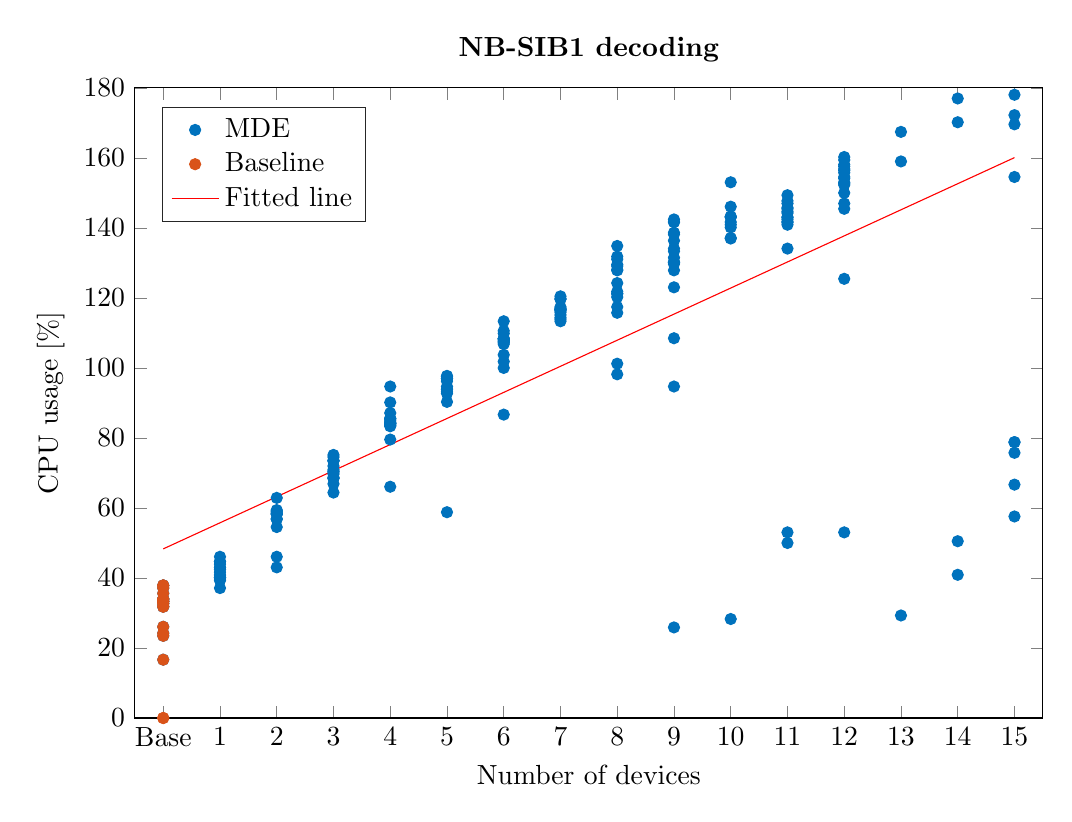
\begin{tikzpicture}

\begin{axis}[%
width=0.951\textwidth,
height=0.66\textwidth,
at={(0\textwidth,0\textwidth)},
scale only axis,
xmin=-0.5,
xmax=15.5,
xtick={0,1,2,3,4,5,6,7,8,9,10,11,12,13,14,15},
xticklabels={{Base},{1},{2},{3},{4},{5},{6},{7},{8},{9},{10},{11},{12},{13},{14},{15}},
xlabel={Number of devices},
ymin=0,
ymax=180,
ylabel={CPU usage [\%]},
axis background/.style={fill=white},
title style={font=\bfseries},
title={NB-SIB1 decoding},
legend style={at={(0.03,0.97)},anchor=north west,legend cell align=left,align=left,draw=white!15!black},
y tick label style={/pgf/number format/fixed}
]
\addplot [color=mycolor1,only marks,mark=*,mark options={solid}]
  table[row sep=crcr]{%
0	32.724\\
1	44.6925\\
4	66.062\\
5	96.97\\
6	86.666\\
7	114.3925\\
8	129.5425\\
9	25.8766666666667\\
11	143.0275\\
12	159.396\\
15	172.21\\
1	40.1475\\
2	58.186\\
3	70.4575\\
4	85.456\\
5	96.97\\
6	106.8175\\
8	117.4225\\
9	108.482\\
10	143.1775\\
11	145.454\\
12	157.578\\
14	40.9075\\
0	16.665\\
1	39.39\\
2	46.064\\
3	73.4875\\
4	90.1525\\
5	92.728\\
6	110.605\\
7	116.362\\
8	127.876\\
9	131.4825\\
10	140.905\\
11	149.342\\
12	158.074\\
15	57.5733333333333\\
0	33.33\\
1	41.6625\\
2	62.8825\\
3	68.488\\
5	96.2125\\
6	108.3325\\
7	115.9075\\
8	124.24\\
9	123.028\\
10	141.6625\\
11	143.07\\
12	154.55\\
15	169.5875\\
0	31.815\\
1	42.42\\
2	56.8225\\
3	71.9725\\
5	58.788\\
6	108.3325\\
9	127.876\\
12	156.8225\\
13	158.986\\
0	23.4825\\
1	39.996\\
2	54.548\\
3	73.4875\\
4	84.0925\\
6	100\\
7	116.665\\
8	98.18\\
11	134.09\\
12	125.456\\
15	154.546\\
0	33.33\\
1	40.1475\\
4	84.85\\
7	116.665\\
8	121.21\\
9	129.694\\
11	147.722\\
12	155.76\\
3	74.548\\
4	87.1225\\
5	97.576\\
6	107.575\\
9	138.635\\
10	136.966\\
11	142.424\\
14	170.18\\
15	66.665\\
0	32.724\\
1	40.602\\
2	59.095\\
3	68.736\\
4	83.638\\
5	93.1825\\
6	113.332\\
8	115.756\\
9	130.14\\
11	146.9725\\
12	53.03\\
0	34.0875\\
2	43.034\\
3	69.7\\
6	103.7425\\
8	120.23\\
9	141.665\\
11	140.9075\\
0	33.936\\
2	58.3375\\
3	75.154\\
4	84.35\\
6	107.878\\
7	113.938\\
9	133.33\\
10	140.1475\\
11	145.7675\\
12	146.97\\
14	176.972\\
0	24.24\\
1	46.056\\
3	68.486\\
4	83.335\\
5	93.94\\
7	120.4525\\
8	101.21\\
9	130.104\\
10	153.0325\\
11	144.695\\
12	160.25\\
0	33.936\\
1	40.905\\
4	85.456\\
5	94.6975\\
6	108.3325\\
7	113.332\\
10	143.25\\
12	156.3975\\
15	178.03\\
0	33.33\\
1	37.1175\\
3	70.912\\
4	83.638\\
5	90.304\\
6	101.818\\
7	117.4225\\
8	129.088\\
9	138.18\\
10	28.28\\
11	53.03\\
0	37.875\\
1	43.026\\
2	59.398\\
4	85.6075\\
7	117.022\\
8	121.21\\
9	94.695\\
11	141.6625\\
12	152.73\\
13	167.4275\\
15	78.79\\
0	31.815\\
1	44.6925\\
4	84.244\\
6	107.272\\
7	116.665\\
8	131.0575\\
9	142.42\\
10	137.1175\\
11	50\\
12	150.0025\\
15	75.755\\
0	37.1175\\
1	43.935\\
2	58.792\\
3	64.395\\
4	79.5475\\
8	128.0275\\
9	130.3\\
10	146.06\\
12	152.275\\
14	50.5033333333333\\
0	35.6025\\
1	39.39\\
2	58.3375\\
3	73.4875\\
4	94.6975\\
7	119.695\\
8	131.815\\
9	136.36\\
10	143.026\\
12	145.456\\
15	78.79\\
0	37.875\\
1	43.026\\
2	56.8225\\
3	70.306\\
4	84.0925\\
5	93.94\\
6	109.8475\\
7	115.15\\
8	121.816\\
9	141.6625\\
11	141.6625\\
12	154.145\\
0	26.058\\
3	66.884\\
4	84.0925\\
5	97.7275\\
6	108.3325\\
7	119.695\\
8	134.845\\
9	134.0875\\
11	144.242\\
12	153.0325\\
13	29.29\\
};
\addlegendentry{MDE};

\addplot [color=mycolor2,only marks,mark=*,mark options={solid}]
  table[row sep=crcr]{%
0	32.724\\
0	0\\
0	16.665\\
0	33.33\\
0	31.815\\
0	23.4825\\
0	33.33\\
0	0\\
0	32.724\\
0	34.0875\\
0	33.936\\
0	24.24\\
0	33.936\\
0	33.33\\
0	37.875\\
0	31.815\\
0	37.1175\\
0	35.6025\\
0	37.875\\
0	26.058\\
};
\addlegendentry{Baseline};

\addplot [color=red,solid]
  table[row sep=crcr]{%
0	48.3088840864026\\
0.015	48.4206481298781\\
0.03	48.5324121733536\\
0.045	48.6441762168291\\
0.06	48.7559402603046\\
0.075	48.8677043037801\\
0.09	48.9794683472556\\
0.105	49.0912323907311\\
0.12	49.2029964342066\\
0.135	49.3147604776821\\
0.15	49.4265245211577\\
0.165	49.5382885646332\\
0.18	49.6500526081087\\
0.195	49.7618166515842\\
0.21	49.8735806950597\\
0.225	49.9853447385352\\
0.24	50.0971087820107\\
0.255	50.2088728254862\\
0.27	50.3206368689617\\
0.285	50.4324009124372\\
0.3	50.5441649559127\\
0.315	50.6559289993883\\
0.33	50.7676930428638\\
0.345	50.8794570863393\\
0.36	50.9912211298148\\
0.375	51.1029851732903\\
0.39	51.2147492167658\\
0.405	51.3265132602413\\
0.42	51.4382773037168\\
0.435	51.5500413471923\\
0.45	51.6618053906678\\
0.465	51.7735694341434\\
0.48	51.8853334776189\\
0.495	51.9970975210944\\
0.51	52.1088615645699\\
0.525	52.2206256080454\\
0.54	52.3323896515209\\
0.555	52.4441536949964\\
0.57	52.5559177384719\\
0.585	52.6676817819474\\
0.6	52.7794458254229\\
0.615	52.8912098688985\\
0.63	53.002973912374\\
0.645	53.1147379558495\\
0.66	53.226501999325\\
0.675	53.3382660428005\\
0.69	53.450030086276\\
0.705	53.5617941297515\\
0.72	53.673558173227\\
0.735	53.7853222167025\\
0.75	53.897086260178\\
0.765	54.0088503036535\\
0.78	54.1206143471291\\
0.795	54.2323783906046\\
0.81	54.3441424340801\\
0.825	54.4559064775556\\
0.84	54.5676705210311\\
0.855	54.6794345645066\\
0.87	54.7911986079821\\
0.885	54.9029626514576\\
0.9	55.0147266949331\\
0.915	55.1264907384086\\
0.93	55.2382547818842\\
0.945	55.3500188253597\\
0.96	55.4617828688352\\
0.975	55.5735469123107\\
0.99	55.6853109557862\\
1.005	55.7970749992617\\
1.02	55.9088390427372\\
1.035	56.0206030862127\\
1.05	56.1323671296882\\
1.065	56.2441311731637\\
1.08	56.3558952166392\\
1.095	56.4676592601148\\
1.11	56.5794233035903\\
1.125	56.6911873470658\\
1.14	56.8029513905413\\
1.155	56.9147154340168\\
1.17	57.0264794774923\\
1.185	57.1382435209678\\
1.2	57.2500075644433\\
1.215	57.3617716079188\\
1.23	57.4735356513943\\
1.245	57.5852996948699\\
1.26	57.6970637383454\\
1.275	57.8088277818209\\
1.29	57.9205918252964\\
1.305	58.0323558687719\\
1.32	58.1441199122474\\
1.335	58.2558839557229\\
1.35	58.3676479991984\\
1.365	58.4794120426739\\
1.38	58.5911760861494\\
1.395	58.7029401296249\\
1.41	58.8147041731005\\
1.425	58.926468216576\\
1.44	59.0382322600515\\
1.455	59.149996303527\\
1.47	59.2617603470025\\
1.485	59.373524390478\\
1.5	59.4852884339535\\
1.515	59.597052477429\\
1.53	59.7088165209045\\
1.545	59.82058056438\\
1.56	59.9323446078556\\
1.575	60.0441086513311\\
1.59	60.1558726948066\\
1.605	60.2676367382821\\
1.62	60.3794007817576\\
1.635	60.4911648252331\\
1.65	60.6029288687086\\
1.665	60.7146929121841\\
1.68	60.8264569556596\\
1.695	60.9382209991351\\
1.71	61.0499850426107\\
1.725	61.1617490860862\\
1.74	61.2735131295617\\
1.755	61.3852771730372\\
1.77	61.4970412165127\\
1.785	61.6088052599882\\
1.8	61.7205693034637\\
1.815	61.8323333469392\\
1.83	61.9440973904147\\
1.845	62.0558614338902\\
1.86	62.1676254773657\\
1.875	62.2793895208413\\
1.89	62.3911535643168\\
1.905	62.5029176077923\\
1.92	62.6146816512678\\
1.935	62.7264456947433\\
1.95	62.8382097382188\\
1.965	62.9499737816943\\
1.98	63.0617378251698\\
1.995	63.1735018686453\\
2.01	63.2852659121208\\
2.025	63.3970299555964\\
2.04	63.5087939990719\\
2.055	63.6205580425474\\
2.07	63.7323220860229\\
2.085	63.8440861294984\\
2.1	63.9558501729739\\
2.115	64.0676142164494\\
2.13	64.1793782599249\\
2.145	64.2911423034004\\
2.16	64.4029063468759\\
2.175	64.5146703903514\\
2.19	64.626434433827\\
2.205	64.7381984773025\\
2.22	64.849962520778\\
2.235	64.9617265642535\\
2.25	65.073490607729\\
2.265	65.1852546512045\\
2.28	65.29701869468\\
2.295	65.4087827381555\\
2.31	65.520546781631\\
2.325	65.6323108251065\\
2.34	65.744074868582\\
2.355	65.8558389120576\\
2.37	65.9676029555331\\
2.385	66.0793669990086\\
2.4	66.1911310424841\\
2.415	66.3028950859596\\
2.43	66.4146591294351\\
2.445	66.5264231729106\\
2.46	66.6381872163861\\
2.475	66.7499512598616\\
2.49	66.8617153033371\\
2.505	66.9734793468127\\
2.52	67.0852433902882\\
2.535	67.1970074337637\\
2.55	67.3087714772392\\
2.565	67.4205355207147\\
2.58	67.5322995641902\\
2.595	67.6440636076657\\
2.61	67.7558276511412\\
2.625	67.8675916946167\\
2.64	67.9793557380922\\
2.655	68.0911197815678\\
2.67	68.2028838250433\\
2.685	68.3146478685188\\
2.7	68.4264119119943\\
2.715	68.5381759554698\\
2.73	68.6499399989453\\
2.745	68.7617040424208\\
2.76	68.8734680858963\\
2.775	68.9852321293718\\
2.79	69.0969961728473\\
2.805	69.2087602163228\\
2.82	69.3205242597984\\
2.835	69.4322883032739\\
2.85	69.5440523467494\\
2.865	69.6558163902249\\
2.88	69.7675804337004\\
2.895	69.8793444771759\\
2.91	69.9911085206514\\
2.925	70.1028725641269\\
2.94	70.2146366076024\\
2.955	70.3264006510779\\
2.97	70.4381646945535\\
2.985	70.549928738029\\
3	70.6616927815045\\
3.015	70.77345682498\\
3.03	70.8852208684555\\
3.045	70.996984911931\\
3.06	71.1087489554065\\
3.075	71.220512998882\\
3.09	71.3322770423575\\
3.105	71.444041085833\\
3.12	71.5558051293086\\
3.135	71.6675691727841\\
3.15	71.7793332162596\\
3.165	71.8910972597351\\
3.18	72.0028613032106\\
3.195	72.1146253466861\\
3.21	72.2263893901616\\
3.225	72.3381534336371\\
3.24	72.4499174771126\\
3.255	72.5616815205881\\
3.27	72.6734455640636\\
3.285	72.7852096075391\\
3.3	72.8969736510147\\
3.315	73.0087376944902\\
3.33	73.1205017379657\\
3.345	73.2322657814412\\
3.36	73.3440298249167\\
3.375	73.4557938683922\\
3.39	73.5675579118677\\
3.405	73.6793219553432\\
3.42	73.7910859988187\\
3.435	73.9028500422942\\
3.45	74.0146140857698\\
3.465	74.1263781292453\\
3.48	74.2381421727208\\
3.495	74.3499062161963\\
3.51	74.4616702596718\\
3.525	74.5734343031473\\
3.54	74.6851983466228\\
3.555	74.7969623900983\\
3.57	74.9087264335738\\
3.585	75.0204904770494\\
3.6	75.1322545205249\\
3.615	75.2440185640004\\
3.63	75.3557826074759\\
3.645	75.4675466509514\\
3.66	75.5793106944269\\
3.675	75.6910747379024\\
3.69	75.8028387813779\\
3.705	75.9146028248534\\
3.72	76.0263668683289\\
3.735	76.1381309118044\\
3.75	76.24989495528\\
3.765	76.3616589987555\\
3.78	76.473423042231\\
3.795	76.5851870857065\\
3.81	76.696951129182\\
3.825	76.8087151726575\\
3.84	76.920479216133\\
3.855	77.0322432596085\\
3.87	77.144007303084\\
3.885	77.2557713465595\\
3.9	77.367535390035\\
3.915	77.4792994335106\\
3.93	77.5910634769861\\
3.945	77.7028275204616\\
3.96	77.8145915639371\\
3.975	77.9263556074126\\
3.99	78.0381196508881\\
4.005	78.1498836943636\\
4.02	78.2616477378391\\
4.035	78.3734117813146\\
4.05	78.4851758247901\\
4.065	78.5969398682657\\
4.08	78.7087039117412\\
4.095	78.8204679552167\\
4.11	78.9322319986922\\
4.125	79.0439960421677\\
4.14	79.1557600856432\\
4.155	79.2675241291187\\
4.17	79.3792881725942\\
4.185	79.4910522160697\\
4.2	79.6028162595452\\
4.215	79.7145803030208\\
4.23	79.8263443464963\\
4.245	79.9381083899718\\
4.26	80.0498724334473\\
4.275	80.1616364769228\\
4.29	80.2734005203983\\
4.305	80.3851645638738\\
4.32	80.4969286073493\\
4.335	80.6086926508248\\
4.35	80.7204566943003\\
4.365	80.8322207377759\\
4.38	80.9439847812513\\
4.395	81.0557488247269\\
4.41	81.1675128682024\\
4.425	81.2792769116779\\
4.44	81.3910409551534\\
4.455	81.5028049986289\\
4.47	81.6145690421044\\
4.485	81.7263330855799\\
4.5	81.8380971290554\\
4.515	81.9498611725309\\
4.53	82.0616252160065\\
4.545	82.173389259482\\
4.56	82.2851533029575\\
4.575	82.396917346433\\
4.59	82.5086813899085\\
4.605	82.620445433384\\
4.62	82.7322094768595\\
4.635	82.843973520335\\
4.65	82.9557375638105\\
4.665	83.067501607286\\
4.68	83.1792656507616\\
4.695	83.2910296942371\\
4.71	83.4027937377126\\
4.725	83.5145577811881\\
4.74	83.6263218246636\\
4.755	83.7380858681391\\
4.77	83.8498499116146\\
4.785	83.9616139550901\\
4.8	84.0733779985656\\
4.815	84.1851420420411\\
4.83	84.2969060855166\\
4.845	84.4086701289922\\
4.86	84.5204341724677\\
4.875	84.6321982159432\\
4.89	84.7439622594187\\
4.905	84.8557263028942\\
4.92	84.9674903463697\\
4.935	85.0792543898452\\
4.95	85.1910184333207\\
4.965	85.3027824767962\\
4.98	85.4145465202717\\
4.995	85.5263105637472\\
5.01	85.6380746072228\\
5.025	85.7498386506983\\
5.04	85.8616026941738\\
5.055	85.9733667376493\\
5.07	86.0851307811248\\
5.085	86.1968948246003\\
5.1	86.3086588680758\\
5.115	86.4204229115513\\
5.13	86.5321869550268\\
5.145	86.6439509985023\\
5.16	86.7557150419779\\
5.175	86.8674790854534\\
5.19	86.9792431289289\\
5.205	87.0910071724044\\
5.22	87.2027712158799\\
5.235	87.3145352593554\\
5.25	87.4262993028309\\
5.265	87.5380633463064\\
5.28	87.6498273897819\\
5.295	87.7615914332574\\
5.31	87.8733554767329\\
5.325	87.9851195202085\\
5.34	88.096883563684\\
5.355	88.2086476071595\\
5.37	88.320411650635\\
5.385	88.4321756941105\\
5.4	88.543939737586\\
5.415	88.6557037810615\\
5.43	88.767467824537\\
5.445	88.8792318680125\\
5.46	88.990995911488\\
5.475	89.1027599549635\\
5.49	89.2145239984391\\
5.505	89.3262880419146\\
5.52	89.4380520853901\\
5.535	89.5498161288656\\
5.55	89.6615801723411\\
5.565	89.7733442158166\\
5.58	89.8851082592921\\
5.595	89.9968723027676\\
5.61	90.1086363462431\\
5.625	90.2204003897186\\
5.64	90.3321644331942\\
5.655	90.4439284766697\\
5.67	90.5556925201452\\
5.685	90.6674565636207\\
5.7	90.7792206070962\\
5.715	90.8909846505717\\
5.73	91.0027486940472\\
5.745	91.1145127375227\\
5.76	91.2262767809982\\
5.775	91.3380408244738\\
5.79	91.4498048679493\\
5.805	91.5615689114248\\
5.82	91.6733329549003\\
5.835	91.7850969983758\\
5.85	91.8968610418513\\
5.865	92.0086250853268\\
5.88	92.1203891288023\\
5.895	92.2321531722778\\
5.91	92.3439172157533\\
5.925	92.4556812592288\\
5.94	92.5674453027044\\
5.955	92.6792093461799\\
5.97	92.7909733896554\\
5.985	92.9027374331309\\
6	93.0145014766064\\
6.015	93.1262655200819\\
6.03	93.2380295635574\\
6.045	93.3497936070329\\
6.06	93.4615576505084\\
6.075	93.5733216939839\\
6.09	93.6850857374594\\
6.105	93.796849780935\\
6.12	93.9086138244105\\
6.135	94.020377867886\\
6.15	94.1321419113615\\
6.165	94.243905954837\\
6.18	94.3556699983125\\
6.195	94.467434041788\\
6.21	94.5791980852635\\
6.225	94.690962128739\\
6.24	94.8027261722145\\
6.255	94.9144902156901\\
6.27	95.0262542591656\\
6.285	95.1380183026411\\
6.3	95.2497823461166\\
6.315	95.3615463895921\\
6.33	95.4733104330676\\
6.345	95.5850744765431\\
6.36	95.6968385200186\\
6.375	95.8086025634941\\
6.39	95.9203666069696\\
6.405	96.0321306504451\\
6.42	96.1438946939207\\
6.435	96.2556587373962\\
6.45	96.3674227808717\\
6.465	96.4791868243472\\
6.48	96.5909508678227\\
6.495	96.7027149112982\\
6.51	96.8144789547737\\
6.525	96.9262429982492\\
6.54	97.0380070417247\\
6.555	97.1497710852002\\
6.57	97.2615351286757\\
6.585	97.3732991721513\\
6.6	97.4850632156268\\
6.615	97.5968272591023\\
6.63	97.7085913025778\\
6.645	97.8203553460533\\
6.66	97.9321193895288\\
6.675	98.0438834330043\\
6.69	98.1556474764798\\
6.705	98.2674115199553\\
6.72	98.3791755634308\\
6.735	98.4909396069064\\
6.75	98.6027036503819\\
6.765	98.7144676938574\\
6.78	98.8262317373329\\
6.795	98.9379957808084\\
6.81	99.0497598242839\\
6.825	99.1615238677594\\
6.84	99.2732879112349\\
6.855	99.3850519547104\\
6.87	99.496815998186\\
6.885	99.6085800416615\\
6.9	99.720344085137\\
6.915	99.8321081286125\\
6.93	99.943872172088\\
6.945	100.055636215563\\
6.96	100.167400259039\\
6.975	100.279164302515\\
6.99	100.39092834599\\
7.005	100.502692389466\\
7.02	100.614456432941\\
7.035	100.726220476417\\
7.05	100.837984519892\\
7.065	100.949748563368\\
7.08	101.061512606843\\
7.095	101.173276650319\\
7.11	101.285040693794\\
7.125	101.39680473727\\
7.14	101.508568780745\\
7.155	101.620332824221\\
7.17	101.732096867696\\
7.185	101.843860911172\\
7.2	101.955624954647\\
7.215	102.067388998123\\
7.23	102.179153041598\\
7.245	102.290917085074\\
7.26	102.402681128549\\
7.275	102.514445172025\\
7.29	102.6262092155\\
7.305	102.737973258976\\
7.32	102.849737302451\\
7.335	102.961501345927\\
7.35	103.073265389402\\
7.365	103.185029432878\\
7.38	103.296793476353\\
7.395	103.408557519829\\
7.41	103.520321563304\\
7.425	103.63208560678\\
7.44	103.743849650255\\
7.455	103.855613693731\\
7.47	103.967377737206\\
7.485	104.079141780682\\
7.5	104.190905824157\\
7.515	104.302669867633\\
7.53	104.414433911108\\
7.545	104.526197954584\\
7.56	104.637961998059\\
7.575	104.749726041535\\
7.59	104.86149008501\\
7.605	104.973254128486\\
7.62	105.085018171961\\
7.635	105.196782215437\\
7.65	105.308546258912\\
7.665	105.420310302388\\
7.68	105.532074345863\\
7.695	105.643838389339\\
7.71	105.755602432814\\
7.725	105.86736647629\\
7.74	105.979130519766\\
7.755	106.090894563241\\
7.77	106.202658606717\\
7.785	106.314422650192\\
7.8	106.426186693668\\
7.815	106.537950737143\\
7.83	106.649714780619\\
7.845	106.761478824094\\
7.86	106.87324286757\\
7.875	106.985006911045\\
7.89	107.096770954521\\
7.905	107.208534997996\\
7.92	107.320299041472\\
7.935	107.432063084947\\
7.95	107.543827128423\\
7.965	107.655591171898\\
7.98	107.767355215374\\
7.995	107.879119258849\\
8.01	107.990883302325\\
8.025	108.1026473458\\
8.04	108.214411389276\\
8.055	108.326175432751\\
8.07	108.437939476227\\
8.085	108.549703519702\\
8.1	108.661467563178\\
8.115	108.773231606653\\
8.13	108.884995650129\\
8.145	108.996759693604\\
8.16	109.10852373708\\
8.175	109.220287780555\\
8.19	109.332051824031\\
8.205	109.443815867506\\
8.22	109.555579910982\\
8.235	109.667343954457\\
8.25	109.779107997933\\
8.265	109.890872041408\\
8.28	110.002636084884\\
8.295	110.114400128359\\
8.31	110.226164171835\\
8.325	110.33792821531\\
8.34	110.449692258786\\
8.355	110.561456302261\\
8.37	110.673220345737\\
8.385	110.784984389212\\
8.4	110.896748432688\\
8.415	111.008512476163\\
8.43	111.120276519639\\
8.445	111.232040563114\\
8.46	111.34380460659\\
8.475	111.455568650065\\
8.49	111.567332693541\\
8.505	111.679096737016\\
8.52	111.790860780492\\
8.535	111.902624823968\\
8.55	112.014388867443\\
8.565	112.126152910919\\
8.58	112.237916954394\\
8.595	112.34968099787\\
8.61	112.461445041345\\
8.625	112.573209084821\\
8.64	112.684973128296\\
8.655	112.796737171772\\
8.67	112.908501215247\\
8.685	113.020265258723\\
8.7	113.132029302198\\
8.715	113.243793345674\\
8.73	113.355557389149\\
8.745	113.467321432625\\
8.76	113.5790854761\\
8.775	113.690849519576\\
8.79	113.802613563051\\
8.805	113.914377606527\\
8.82	114.026141650002\\
8.835	114.137905693478\\
8.85	114.249669736953\\
8.865	114.361433780429\\
8.88	114.473197823904\\
8.895	114.58496186738\\
8.91	114.696725910855\\
8.925	114.808489954331\\
8.94	114.920253997806\\
8.955	115.032018041282\\
8.97	115.143782084757\\
8.985	115.255546128233\\
9	115.367310171708\\
9.015	115.479074215184\\
9.03	115.590838258659\\
9.045	115.702602302135\\
9.06	115.81436634561\\
9.075	115.926130389086\\
9.09	116.037894432561\\
9.105	116.149658476037\\
9.12	116.261422519512\\
9.135	116.373186562988\\
9.15	116.484950606463\\
9.165	116.596714649939\\
9.18	116.708478693414\\
9.195	116.82024273689\\
9.21	116.932006780365\\
9.225	117.043770823841\\
9.24	117.155534867316\\
9.255	117.267298910792\\
9.27	117.379062954267\\
9.285	117.490826997743\\
9.3	117.602591041218\\
9.315	117.714355084694\\
9.33	117.82611912817\\
9.345	117.937883171645\\
9.36	118.049647215121\\
9.375	118.161411258596\\
9.39	118.273175302072\\
9.405	118.384939345547\\
9.42	118.496703389023\\
9.435	118.608467432498\\
9.45	118.720231475974\\
9.465	118.831995519449\\
9.48	118.943759562925\\
9.495	119.0555236064\\
9.51	119.167287649876\\
9.525	119.279051693351\\
9.54	119.390815736827\\
9.555	119.502579780302\\
9.57	119.614343823778\\
9.585	119.726107867253\\
9.6	119.837871910729\\
9.615	119.949635954204\\
9.63	120.06139999768\\
9.645	120.173164041155\\
9.66	120.284928084631\\
9.675	120.396692128106\\
9.69	120.508456171582\\
9.705	120.620220215057\\
9.72	120.731984258533\\
9.735	120.843748302008\\
9.75	120.955512345484\\
9.765	121.067276388959\\
9.78	121.179040432435\\
9.795	121.29080447591\\
9.81	121.402568519386\\
9.825	121.514332562861\\
9.84	121.626096606337\\
9.855	121.737860649812\\
9.87	121.849624693288\\
9.885	121.961388736763\\
9.9	122.073152780239\\
9.915	122.184916823714\\
9.93	122.29668086719\\
9.945	122.408444910665\\
9.96	122.520208954141\\
9.975	122.631972997616\\
9.99	122.743737041092\\
10.005	122.855501084567\\
10.02	122.967265128043\\
10.035	123.079029171518\\
10.05	123.190793214994\\
10.065	123.302557258469\\
10.08	123.414321301945\\
10.095	123.526085345421\\
10.11	123.637849388896\\
10.125	123.749613432372\\
10.14	123.861377475847\\
10.155	123.973141519323\\
10.17	124.084905562798\\
10.185	124.196669606274\\
10.2	124.308433649749\\
10.215	124.420197693225\\
10.23	124.5319617367\\
10.245	124.643725780176\\
10.26	124.755489823651\\
10.275	124.867253867127\\
10.29	124.979017910602\\
10.305	125.090781954078\\
10.32	125.202545997553\\
10.335	125.314310041029\\
10.35	125.426074084504\\
10.365	125.53783812798\\
10.38	125.649602171455\\
10.395	125.761366214931\\
10.41	125.873130258406\\
10.425	125.984894301882\\
10.44	126.096658345357\\
10.455	126.208422388833\\
10.47	126.320186432308\\
10.485	126.431950475784\\
10.5	126.543714519259\\
10.515	126.655478562735\\
10.53	126.76724260621\\
10.545	126.879006649686\\
10.56	126.990770693161\\
10.575	127.102534736637\\
10.59	127.214298780112\\
10.605	127.326062823588\\
10.62	127.437826867063\\
10.635	127.549590910539\\
10.65	127.661354954014\\
10.665	127.77311899749\\
10.68	127.884883040965\\
10.695	127.996647084441\\
10.71	128.108411127916\\
10.725	128.220175171392\\
10.74	128.331939214867\\
10.755	128.443703258343\\
10.77	128.555467301818\\
10.785	128.667231345294\\
10.8	128.778995388769\\
10.815	128.890759432245\\
10.83	129.00252347572\\
10.845	129.114287519196\\
10.86	129.226051562672\\
10.875	129.337815606147\\
10.89	129.449579649623\\
10.905	129.561343693098\\
10.92	129.673107736574\\
10.935	129.784871780049\\
10.95	129.896635823525\\
10.965	130.008399867\\
10.98	130.120163910476\\
10.995	130.231927953951\\
11.01	130.343691997427\\
11.025	130.455456040902\\
11.04	130.567220084378\\
11.055	130.678984127853\\
11.07	130.790748171329\\
11.085	130.902512214804\\
11.1	131.01427625828\\
11.115	131.126040301755\\
11.13	131.237804345231\\
11.145	131.349568388706\\
11.16	131.461332432182\\
11.175	131.573096475657\\
11.19	131.684860519133\\
11.205	131.796624562608\\
11.22	131.908388606084\\
11.235	132.020152649559\\
11.25	132.131916693035\\
11.265	132.24368073651\\
11.28	132.355444779986\\
11.295	132.467208823461\\
11.31	132.578972866937\\
11.325	132.690736910412\\
11.34	132.802500953888\\
11.355	132.914264997363\\
11.37	133.026029040839\\
11.385	133.137793084314\\
11.4	133.24955712779\\
11.415	133.361321171265\\
11.43	133.473085214741\\
11.445	133.584849258216\\
11.46	133.696613301692\\
11.475	133.808377345167\\
11.49	133.920141388643\\
11.505	134.031905432118\\
11.52	134.143669475594\\
11.535	134.255433519069\\
11.55	134.367197562545\\
11.565	134.47896160602\\
11.58	134.590725649496\\
11.595	134.702489692971\\
11.61	134.814253736447\\
11.625	134.926017779922\\
11.64	135.037781823398\\
11.655	135.149545866874\\
11.67	135.261309910349\\
11.685	135.373073953825\\
11.7	135.4848379973\\
11.715	135.596602040776\\
11.73	135.708366084251\\
11.745	135.820130127727\\
11.76	135.931894171202\\
11.775	136.043658214678\\
11.79	136.155422258153\\
11.805	136.267186301629\\
11.82	136.378950345104\\
11.835	136.49071438858\\
11.85	136.602478432055\\
11.865	136.714242475531\\
11.88	136.826006519006\\
11.895	136.937770562482\\
11.91	137.049534605957\\
11.925	137.161298649433\\
11.94	137.273062692908\\
11.955	137.384826736384\\
11.97	137.496590779859\\
11.985	137.608354823335\\
12	137.72011886681\\
12.015	137.831882910286\\
12.03	137.943646953761\\
12.045	138.055410997237\\
12.06	138.167175040712\\
12.075	138.278939084188\\
12.09	138.390703127663\\
12.105	138.502467171139\\
12.12	138.614231214614\\
12.135	138.72599525809\\
12.15	138.837759301565\\
12.165	138.949523345041\\
12.18	139.061287388516\\
12.195	139.173051431992\\
12.21	139.284815475467\\
12.225	139.396579518943\\
12.24	139.508343562418\\
12.255	139.620107605894\\
12.27	139.731871649369\\
12.285	139.843635692845\\
12.3	139.95539973632\\
12.315	140.067163779796\\
12.33	140.178927823271\\
12.345	140.290691866747\\
12.36	140.402455910222\\
12.375	140.514219953698\\
12.39	140.625983997173\\
12.405	140.737748040649\\
12.42	140.849512084124\\
12.435	140.9612761276\\
12.45	141.073040171075\\
12.465	141.184804214551\\
12.48	141.296568258027\\
12.495	141.408332301502\\
12.51	141.520096344978\\
12.525	141.631860388453\\
12.54	141.743624431929\\
12.555	141.855388475404\\
12.57	141.96715251888\\
12.585	142.078916562355\\
12.6	142.190680605831\\
12.615	142.302444649306\\
12.63	142.414208692782\\
12.645	142.525972736257\\
12.66	142.637736779733\\
12.675	142.749500823208\\
12.69	142.861264866684\\
12.705	142.973028910159\\
12.72	143.084792953635\\
12.735	143.19655699711\\
12.75	143.308321040586\\
12.765	143.420085084061\\
12.78	143.531849127537\\
12.795	143.643613171012\\
12.81	143.755377214488\\
12.825	143.867141257963\\
12.84	143.978905301439\\
12.855	144.090669344914\\
12.87	144.20243338839\\
12.885	144.314197431865\\
12.9	144.425961475341\\
12.915	144.537725518816\\
12.93	144.649489562292\\
12.945	144.761253605767\\
12.96	144.873017649243\\
12.975	144.984781692718\\
12.99	145.096545736194\\
13.005	145.208309779669\\
13.02	145.320073823145\\
13.035	145.43183786662\\
13.05	145.543601910096\\
13.065	145.655365953571\\
13.08	145.767129997047\\
13.095	145.878894040522\\
13.11	145.990658083998\\
13.125	146.102422127473\\
13.14	146.214186170949\\
13.155	146.325950214424\\
13.17	146.4377142579\\
13.185	146.549478301375\\
13.2	146.661242344851\\
13.215	146.773006388327\\
13.23	146.884770431802\\
13.245	146.996534475278\\
13.26	147.108298518753\\
13.275	147.220062562229\\
13.29	147.331826605704\\
13.305	147.44359064918\\
13.32	147.555354692655\\
13.335	147.667118736131\\
13.35	147.778882779606\\
13.365	147.890646823082\\
13.38	148.002410866557\\
13.395	148.114174910033\\
13.41	148.225938953508\\
13.425	148.337702996984\\
13.44	148.449467040459\\
13.455	148.561231083935\\
13.47	148.67299512741\\
13.485	148.784759170886\\
13.5	148.896523214361\\
13.515	149.008287257837\\
13.53	149.120051301312\\
13.545	149.231815344788\\
13.56	149.343579388263\\
13.575	149.455343431739\\
13.59	149.567107475214\\
13.605	149.67887151869\\
13.62	149.790635562165\\
13.635	149.902399605641\\
13.65	150.014163649116\\
13.665	150.125927692592\\
13.68	150.237691736067\\
13.695	150.349455779543\\
13.71	150.461219823018\\
13.725	150.572983866494\\
13.74	150.684747909969\\
13.755	150.796511953445\\
13.77	150.90827599692\\
13.785	151.020040040396\\
13.8	151.131804083871\\
13.815	151.243568127347\\
13.83	151.355332170822\\
13.845	151.467096214298\\
13.86	151.578860257773\\
13.875	151.690624301249\\
13.89	151.802388344724\\
13.905	151.9141523882\\
13.92	152.025916431675\\
13.935	152.137680475151\\
13.95	152.249444518626\\
13.965	152.361208562102\\
13.98	152.472972605577\\
13.995	152.584736649053\\
14.01	152.696500692529\\
14.025	152.808264736004\\
14.04	152.92002877948\\
14.055	153.031792822955\\
14.07	153.143556866431\\
14.085	153.255320909906\\
14.1	153.367084953382\\
14.115	153.478848996857\\
14.13	153.590613040333\\
14.145	153.702377083808\\
14.16	153.814141127284\\
14.175	153.925905170759\\
14.19	154.037669214235\\
14.205	154.14943325771\\
14.22	154.261197301186\\
14.235	154.372961344661\\
14.25	154.484725388137\\
14.265	154.596489431612\\
14.28	154.708253475088\\
14.295	154.820017518563\\
14.31	154.931781562039\\
14.325	155.043545605514\\
14.34	155.15530964899\\
14.355	155.267073692465\\
14.37	155.378837735941\\
14.385	155.490601779416\\
14.4	155.602365822892\\
14.415	155.714129866367\\
14.43	155.825893909843\\
14.445	155.937657953318\\
14.46	156.049421996794\\
14.475	156.161186040269\\
14.49	156.272950083745\\
14.505	156.38471412722\\
14.52	156.496478170696\\
14.535	156.608242214171\\
14.55	156.720006257647\\
14.565	156.831770301122\\
14.58	156.943534344598\\
14.595	157.055298388073\\
14.61	157.167062431549\\
14.625	157.278826475024\\
14.64	157.3905905185\\
14.655	157.502354561975\\
14.67	157.614118605451\\
14.685	157.725882648926\\
14.7	157.837646692402\\
14.715	157.949410735877\\
14.73	158.061174779353\\
14.745	158.172938822828\\
14.76	158.284702866304\\
14.775	158.396466909779\\
14.79	158.508230953255\\
14.805	158.619994996731\\
14.82	158.731759040206\\
14.835	158.843523083682\\
14.85	158.955287127157\\
14.865	159.067051170633\\
14.88	159.178815214108\\
14.895	159.290579257584\\
14.91	159.402343301059\\
14.925	159.514107344535\\
14.94	159.62587138801\\
14.955	159.737635431486\\
14.97	159.849399474961\\
14.985	159.961163518437\\
15	160.072927561912\\
};
\addlegendentry{Fitted line};

\end{axis}
\end{tikzpicture}%}
\caption{CPU usage for the NB-SIB1 step of the MDE for different number of devices and the baseline emulator. The fitted line is a linear approximation}
\label{fig:CPU_SIB1}
\end{figure}

The fitted line for the CPU usage is estimated to be:
\begin{equation}
CPU_{NB-SIB1} = 9.93 \cdot NoD + 38.92
\end{equation}

As seen on \autoref{fig:CPU_SIB1}, this step also have a higher CPU usage at higher number of devices. It is also seen that the CPU usage is raising above 100\%, but as there is multiple threads in work at this point, multiple kernels is also in use, where the CPU usage for each kernel is added together by the CPU stat tool. As mentioned a limit of seven CPU's are assumed, which gives a upper limit of 700\%. The reason for increase in CPU usage, compared to the previous steps, is that the individual devices is used at this point. In the previous two steps only the Co\_Phy was active.

\subsection{NB-SIB2}
The NB-SIB2 step is measured from the NB-SIB1 is decoded until NB-SIB2 is decoded, which gives the results seen on \autoref{fig:CPU_init}. 

\begin{figure}[H]
\tikzsetnextfilename{CPU_SIB2}
\centering
\resizebox{0.5\textwidth}{!}{
% This file was created by matlab2tikz.
%
%The latest updates can be retrieved from
%  http://www.mathworks.com/matlabcentral/fileexchange/22022-matlab2tikz-matlab2tikz
%where you can also make suggestions and rate matlab2tikz.
%
\definecolor{mycolor1}{rgb}{0.00000,0.44700,0.74100}%
\definecolor{mycolor2}{rgb}{0.85000,0.32500,0.09800}%
%
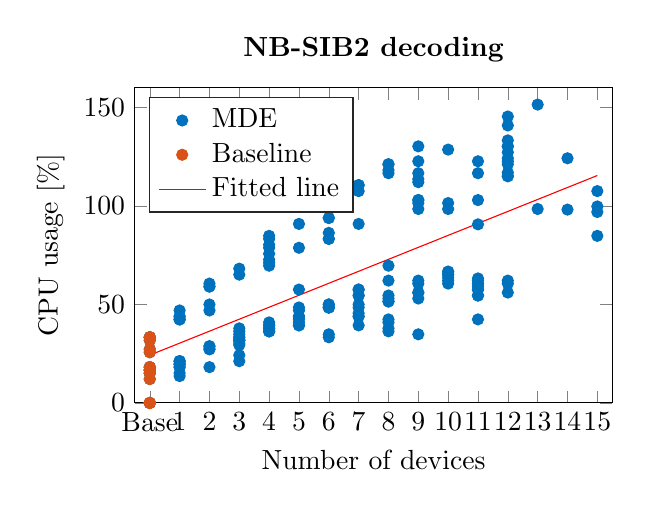
\begin{tikzpicture}

\begin{axis}[%
width=0.5\textwidth,
height=0.33\textwidth,
at={(0\textwidth,0\textwidth)},
scale only axis,
xmin=-0.5,
xmax=15.5,
xtick={0,1,2,3,4,5,6,7,8,9,10,11,12,13,14,15},
xticklabels={{Base},{1},{2},{3},{4},{5},{6},{7},{8},{9},{10},{11},{12},{13},{14},{15}},
xlabel={Number of devices},
ymin=0,
ymax=160,
ylabel={CPU usage [\%]},
axis background/.style={fill=white},
title style={font=\bfseries},
title={NB-SIB2 decoding},
legend style={at={(0.03,0.97)},anchor=north west,legend cell align=left,align=left,draw=white!15!black},
y tick label style={/pgf/number format/fixed}
]
\addplot [color=mycolor1,only marks,mark=*,mark options={solid}]
  table[row sep=crcr]{%
0	12.12\\
1	43.935\\
5	46.97\\
7	50\\
8	118.18\\
11	60.295\\
12	130.3\\
15	96.97\\
1	13.635\\
2	60.61\\
3	34.85\\
4	37.88\\
5	43.94\\
6	50\\
8	37.88\\
10	66.665\\
11	57.575\\
12	127.27\\
1	15.15\\
3	36.365\\
4	80.305\\
5	90.91\\
6	86.365\\
7	43.94\\
8	53.03\\
9	56.06\\
10	98.485\\
11	60.605\\
12	145.45\\
0	16.665\\
1	19.695\\
2	59.095\\
3	31.82\\
5	43.94\\
6	83.335\\
7	48.485\\
8	42.425\\
9	34.85\\
10	66.665\\
11	90.69\\
12	130.305\\
15	99.78\\
0	15.15\\
1	42.42\\
2	46.97\\
3	68.185\\
6	48.485\\
9	103.03\\
12	140.91\\
13	98.485\\
1	19.695\\
2	18.18\\
3	65.155\\
4	40.91\\
6	33.335\\
7	57.575\\
11	42.425\\
15	84.85\\
0	33.33\\
1	19.695\\
4	75.76\\
7	57.575\\
8	36.365\\
9	112.12\\
11	63.235\\
12	133.33\\
3	37.88\\
4	69.7\\
5	39.395\\
6	83.335\\
9	98.485\\
10	62.12\\
11	54.545\\
14	98.175\\
0	16.665\\
1	18.18\\
2	50\\
3	29.41\\
4	36.365\\
5	39.395\\
6	48.485\\
8	69.7\\
9	60.605\\
11	62.12\\
0	27.27\\
3	33.335\\
6	48.485\\
8	40.91\\
9	116.665\\
11	54.545\\
0	16.665\\
2	27.275\\
3	33.335\\
4	78.79\\
6	48.485\\
7	39.395\\
9	103.03\\
10	65.15\\
11	57.575\\
12	62.12\\
14	124.245\\
1	42.42\\
3	24.24\\
4	36.365\\
5	42.425\\
7	110.605\\
9	53.03\\
10	128.65\\
11	122.725\\
12	115.15\\
0	15.15\\
1	21.21\\
4	37.88\\
5	78.79\\
6	50\\
7	43.94\\
10	65.15\\
12	116.98\\
15	107.575\\
0	25.755\\
1	18.18\\
3	31.82\\
4	36.365\\
5	57.58\\
6	34.85\\
7	90.91\\
8	54.545\\
9	56.06\\
0	18.18\\
1	21.21\\
2	28.79\\
4	71.215\\
7	45.59\\
8	51.515\\
11	116.665\\
12	115.15\\
13	151.515\\
0	33.33\\
1	42.42\\
4	39.395\\
6	93.94\\
7	54.545\\
8	116.665\\
9	130.3\\
10	101.515\\
12	122.725\\
0	33.33\\
1	46.97\\
2	28.79\\
3	21.21\\
4	39.395\\
8	62.12\\
9	113.635\\
10	60.605\\
12	60.605\\
0	18.18\\
1	43.94\\
2	59.095\\
3	30.305\\
4	83.335\\
7	110.605\\
8	121.21\\
9	101.515\\
10	63.635\\
12	56.06\\
0	31.815\\
1	21.21\\
2	27.275\\
3	31.82\\
4	84.85\\
5	40.91\\
6	93.94\\
7	54.545\\
8	51.515\\
9	122.725\\
11	103.03\\
12	124.245\\
3	31.82\\
4	72.73\\
5	48.485\\
6	101.515\\
7	107.575\\
8	121.21\\
9	62.12\\
11	59.09\\
12	121.21\\
};
\addlegendentry{MDE};

\addplot [color=mycolor2,only marks,mark=*,mark options={solid}]
  table[row sep=crcr]{%
0	12.12\\
0	0\\
0	0\\
0	16.665\\
0	15.15\\
0	0\\
0	33.33\\
0	0\\
0	16.665\\
0	27.27\\
0	16.665\\
0	0\\
0	15.15\\
0	25.755\\
0	18.18\\
0	33.33\\
0	33.33\\
0	18.18\\
0	31.815\\
0	0\\
};
\addlegendentry{Baseline};

\addplot [color=red,solid]
  table[row sep=crcr]{%
0	24.2822432698915\\
0.015	24.3734563678329\\
0.03	24.4646694657743\\
0.045	24.5558825637157\\
0.06	24.6470956616571\\
0.075	24.7383087595984\\
0.09	24.8295218575398\\
0.105	24.9207349554812\\
0.12	25.0119480534226\\
0.135	25.103161151364\\
0.15	25.1943742493053\\
0.165	25.2855873472467\\
0.18	25.3768004451881\\
0.195	25.4680135431295\\
0.21	25.5592266410708\\
0.225	25.6504397390122\\
0.24	25.7416528369536\\
0.255	25.832865934895\\
0.27	25.9240790328364\\
0.285	26.0152921307777\\
0.3	26.1065052287191\\
0.315	26.1977183266605\\
0.33	26.2889314246019\\
0.345	26.3801445225433\\
0.36	26.4713576204846\\
0.375	26.562570718426\\
0.39	26.6537838163674\\
0.405	26.7449969143088\\
0.42	26.8362100122501\\
0.435	26.9274231101915\\
0.45	27.0186362081329\\
0.465	27.1098493060743\\
0.48	27.2010624040157\\
0.495	27.292275501957\\
0.51	27.3834885998984\\
0.525	27.4747016978398\\
0.54	27.5659147957812\\
0.555	27.6571278937226\\
0.57	27.7483409916639\\
0.585	27.8395540896053\\
0.6	27.9307671875467\\
0.615	28.0219802854881\\
0.63	28.1131933834294\\
0.645	28.2044064813708\\
0.66	28.2956195793122\\
0.675	28.3868326772536\\
0.69	28.478045775195\\
0.705	28.5692588731363\\
0.72	28.6604719710777\\
0.735	28.7516850690191\\
0.75	28.8428981669605\\
0.765	28.9341112649019\\
0.78	29.0253243628432\\
0.795	29.1165374607846\\
0.81	29.207750558726\\
0.825	29.2989636566674\\
0.84	29.3901767546087\\
0.855	29.4813898525501\\
0.87	29.5726029504915\\
0.885	29.6638160484329\\
0.9	29.7550291463743\\
0.915	29.8462422443156\\
0.93	29.937455342257\\
0.945	30.0286684401984\\
0.96	30.1198815381398\\
0.975	30.2110946360812\\
0.99	30.3023077340225\\
1.005	30.3935208319639\\
1.02	30.4847339299053\\
1.035	30.5759470278467\\
1.05	30.667160125788\\
1.065	30.7583732237294\\
1.08	30.8495863216708\\
1.095	30.9407994196122\\
1.11	31.0320125175536\\
1.125	31.1232256154949\\
1.14	31.2144387134363\\
1.155	31.3056518113777\\
1.17	31.3968649093191\\
1.185	31.4880780072605\\
1.2	31.5792911052018\\
1.215	31.6705042031432\\
1.23	31.7617173010846\\
1.245	31.852930399026\\
1.26	31.9441434969673\\
1.275	32.0353565949087\\
1.29	32.1265696928501\\
1.305	32.2177827907915\\
1.32	32.3089958887329\\
1.335	32.4002089866742\\
1.35	32.4914220846156\\
1.365	32.582635182557\\
1.38	32.6738482804984\\
1.395	32.7650613784398\\
1.41	32.8562744763811\\
1.425	32.9474875743225\\
1.44	33.0387006722639\\
1.455	33.1299137702053\\
1.47	33.2211268681466\\
1.485	33.312339966088\\
1.5	33.4035530640294\\
1.515	33.4947661619708\\
1.53	33.5859792599122\\
1.545	33.6771923578535\\
1.56	33.7684054557949\\
1.575	33.8596185537363\\
1.59	33.9508316516777\\
1.605	34.0420447496191\\
1.62	34.1332578475604\\
1.635	34.2244709455018\\
1.65	34.3156840434432\\
1.665	34.4068971413846\\
1.68	34.4981102393259\\
1.695	34.5893233372673\\
1.71	34.6805364352087\\
1.725	34.7717495331501\\
1.74	34.8629626310915\\
1.755	34.9541757290328\\
1.77	35.0453888269742\\
1.785	35.1366019249156\\
1.8	35.227815022857\\
1.815	35.3190281207984\\
1.83	35.4102412187397\\
1.845	35.5014543166811\\
1.86	35.5926674146225\\
1.875	35.6838805125639\\
1.89	35.7750936105052\\
1.905	35.8663067084466\\
1.92	35.957519806388\\
1.935	36.0487329043294\\
1.95	36.1399460022708\\
1.965	36.2311591002121\\
1.98	36.3223721981535\\
1.995	36.4135852960949\\
2.01	36.5047983940363\\
2.025	36.5960114919777\\
2.04	36.687224589919\\
2.055	36.7784376878604\\
2.07	36.8696507858018\\
2.085	36.9608638837432\\
2.1	37.0520769816846\\
2.115	37.1432900796259\\
2.13	37.2345031775673\\
2.145	37.3257162755087\\
2.16	37.4169293734501\\
2.175	37.5081424713914\\
2.19	37.5993555693328\\
2.205	37.6905686672742\\
2.22	37.7817817652156\\
2.235	37.872994863157\\
2.25	37.9642079610983\\
2.265	38.0554210590397\\
2.28	38.1466341569811\\
2.295	38.2378472549225\\
2.31	38.3290603528638\\
2.325	38.4202734508052\\
2.34	38.5114865487466\\
2.355	38.602699646688\\
2.37	38.6939127446294\\
2.385	38.7851258425707\\
2.4	38.8763389405121\\
2.415	38.9675520384535\\
2.43	39.0587651363949\\
2.445	39.1499782343363\\
2.46	39.2411913322776\\
2.475	39.332404430219\\
2.49	39.4236175281604\\
2.505	39.5148306261018\\
2.52	39.6060437240431\\
2.535	39.6972568219845\\
2.55	39.7884699199259\\
2.565	39.8796830178673\\
2.58	39.9708961158087\\
2.595	40.06210921375\\
2.61	40.1533223116914\\
2.625	40.2445354096328\\
2.64	40.3357485075742\\
2.655	40.4269616055156\\
2.67	40.5181747034569\\
2.685	40.6093878013983\\
2.7	40.7006008993397\\
2.715	40.7918139972811\\
2.73	40.8830270952224\\
2.745	40.9742401931638\\
2.76	41.0654532911052\\
2.775	41.1566663890466\\
2.79	41.247879486988\\
2.805	41.3390925849293\\
2.82	41.4303056828707\\
2.835	41.5215187808121\\
2.85	41.6127318787535\\
2.865	41.7039449766949\\
2.88	41.7951580746362\\
2.895	41.8863711725776\\
2.91	41.977584270519\\
2.925	42.0687973684604\\
2.94	42.1600104664017\\
2.955	42.2512235643431\\
2.97	42.3424366622845\\
2.985	42.4336497602259\\
3	42.5248628581673\\
3.015	42.6160759561086\\
3.03	42.70728905405\\
3.045	42.7985021519914\\
3.06	42.8897152499328\\
3.075	42.9809283478742\\
3.09	43.0721414458155\\
3.105	43.1633545437569\\
3.12	43.2545676416983\\
3.135	43.3457807396397\\
3.15	43.436993837581\\
3.165	43.5282069355224\\
3.18	43.6194200334638\\
3.195	43.7106331314052\\
3.21	43.8018462293466\\
3.225	43.8930593272879\\
3.24	43.9842724252293\\
3.255	44.0754855231707\\
3.27	44.1666986211121\\
3.285	44.2579117190535\\
3.3	44.3491248169948\\
3.315	44.4403379149362\\
3.33	44.5315510128776\\
3.345	44.622764110819\\
3.36	44.7139772087603\\
3.375	44.8051903067017\\
3.39	44.8964034046431\\
3.405	44.9876165025845\\
3.42	45.0788296005259\\
3.435	45.1700426984672\\
3.45	45.2612557964086\\
3.465	45.35246889435\\
3.48	45.4436819922914\\
3.495	45.5348950902328\\
3.51	45.6261081881741\\
3.525	45.7173212861155\\
3.54	45.8085343840569\\
3.555	45.8997474819983\\
3.57	45.9909605799396\\
3.585	46.082173677881\\
3.6	46.1733867758224\\
3.615	46.2645998737638\\
3.63	46.3558129717052\\
3.645	46.4470260696465\\
3.66	46.5382391675879\\
3.675	46.6294522655293\\
3.69	46.7206653634707\\
3.705	46.8118784614121\\
3.72	46.9030915593534\\
3.735	46.9943046572948\\
3.75	47.0855177552362\\
3.765	47.1767308531776\\
3.78	47.2679439511189\\
3.795	47.3591570490603\\
3.81	47.4503701470017\\
3.825	47.5415832449431\\
3.84	47.6327963428845\\
3.855	47.7240094408258\\
3.87	47.8152225387672\\
3.885	47.9064356367086\\
3.9	47.99764873465\\
3.915	48.0888618325913\\
3.93	48.1800749305327\\
3.945	48.2712880284741\\
3.96	48.3625011264155\\
3.975	48.4537142243569\\
3.99	48.5449273222982\\
4.005	48.6361404202396\\
4.02	48.727353518181\\
4.035	48.8185666161224\\
4.05	48.9097797140638\\
4.065	49.0009928120051\\
4.08	49.0922059099465\\
4.095	49.1834190078879\\
4.11	49.2746321058293\\
4.125	49.3658452037707\\
4.14	49.457058301712\\
4.155	49.5482713996534\\
4.17	49.6394844975948\\
4.185	49.7306975955362\\
4.2	49.8219106934775\\
4.215	49.9131237914189\\
4.23	50.0043368893603\\
4.245	50.0955499873017\\
4.26	50.1867630852431\\
4.275	50.2779761831844\\
4.29	50.3691892811258\\
4.305	50.4604023790672\\
4.32	50.5516154770086\\
4.335	50.64282857495\\
4.35	50.7340416728913\\
4.365	50.8252547708327\\
4.38	50.9164678687741\\
4.395	51.0076809667155\\
4.41	51.0988940646568\\
4.425	51.1901071625982\\
4.44	51.2813202605396\\
4.455	51.372533358481\\
4.47	51.4637464564224\\
4.485	51.5549595543637\\
4.5	51.6461726523051\\
4.515	51.7373857502465\\
4.53	51.8285988481879\\
4.545	51.9198119461293\\
4.56	52.0110250440706\\
4.575	52.102238142012\\
4.59	52.1934512399534\\
4.605	52.2846643378948\\
4.62	52.3758774358361\\
4.635	52.4670905337775\\
4.65	52.5583036317189\\
4.665	52.6495167296603\\
4.68	52.7407298276017\\
4.695	52.831942925543\\
4.71	52.9231560234844\\
4.725	53.0143691214258\\
4.74	53.1055822193672\\
4.755	53.1967953173086\\
4.77	53.2880084152499\\
4.785	53.3792215131913\\
4.8	53.4704346111327\\
4.815	53.5616477090741\\
4.83	53.6528608070154\\
4.845	53.7440739049568\\
4.86	53.8352870028982\\
4.875	53.9265001008396\\
4.89	54.017713198781\\
4.905	54.1089262967223\\
4.92	54.2001393946637\\
4.935	54.2913524926051\\
4.95	54.3825655905465\\
4.965	54.4737786884879\\
4.98	54.5649917864292\\
4.995	54.6562048843706\\
5.01	54.747417982312\\
5.025	54.8386310802534\\
5.04	54.9298441781947\\
5.055	55.0210572761361\\
5.07	55.1122703740775\\
5.085	55.2034834720189\\
5.1	55.2946965699603\\
5.115	55.3859096679016\\
5.13	55.477122765843\\
5.145	55.5683358637844\\
5.16	55.6595489617258\\
5.175	55.7507620596672\\
5.19	55.8419751576085\\
5.205	55.9331882555499\\
5.22	56.0244013534913\\
5.235	56.1156144514327\\
5.25	56.206827549374\\
5.265	56.2980406473154\\
5.28	56.3892537452568\\
5.295	56.4804668431982\\
5.31	56.5716799411396\\
5.325	56.6628930390809\\
5.34	56.7541061370223\\
5.355	56.8453192349637\\
5.37	56.9365323329051\\
5.385	57.0277454308465\\
5.4	57.1189585287878\\
5.415	57.2101716267292\\
5.43	57.3013847246706\\
5.445	57.392597822612\\
5.46	57.4838109205533\\
5.475	57.5750240184947\\
5.49	57.6662371164361\\
5.505	57.7574502143775\\
5.52	57.8486633123189\\
5.535	57.9398764102602\\
5.55	58.0310895082016\\
5.565	58.122302606143\\
5.58	58.2135157040844\\
5.595	58.3047288020258\\
5.61	58.3959418999671\\
5.625	58.4871549979085\\
5.64	58.5783680958499\\
5.655	58.6695811937913\\
5.67	58.7607942917326\\
5.685	58.852007389674\\
5.7	58.9432204876154\\
5.715	59.0344335855568\\
5.73	59.1256466834982\\
5.745	59.2168597814395\\
5.76	59.3080728793809\\
5.775	59.3992859773223\\
5.79	59.4904990752637\\
5.805	59.581712173205\\
5.82	59.6729252711464\\
5.835	59.7641383690878\\
5.85	59.8553514670292\\
5.865	59.9465645649706\\
5.88	60.037777662912\\
5.895	60.1289907608533\\
5.91	60.2202038587947\\
5.925	60.3114169567361\\
5.94	60.4026300546775\\
5.955	60.4938431526188\\
5.97	60.5850562505602\\
5.985	60.6762693485016\\
6	60.767482446443\\
6.015	60.8586955443843\\
6.03	60.9499086423257\\
6.045	61.0411217402671\\
6.06	61.1323348382085\\
6.075	61.2235479361499\\
6.09	61.3147610340912\\
6.105	61.4059741320326\\
6.12	61.497187229974\\
6.135	61.5884003279154\\
6.15	61.6796134258568\\
6.165	61.7708265237981\\
6.18	61.8620396217395\\
6.195	61.9532527196809\\
6.21	62.0444658176223\\
6.225	62.1356789155636\\
6.24	62.226892013505\\
6.255	62.3181051114464\\
6.27	62.4093182093878\\
6.285	62.5005313073292\\
6.3	62.5917444052705\\
6.315	62.6829575032119\\
6.33	62.7741706011533\\
6.345	62.8653836990947\\
6.36	62.9565967970361\\
6.375	63.0478098949774\\
6.39	63.1390229929188\\
6.405	63.2302360908602\\
6.42	63.3214491888016\\
6.435	63.4126622867429\\
6.45	63.5038753846843\\
6.465	63.5950884826257\\
6.48	63.6863015805671\\
6.495	63.7775146785085\\
6.51	63.8687277764498\\
6.525	63.9599408743912\\
6.54	64.0511539723326\\
6.555	64.142367070274\\
6.57	64.2335801682154\\
6.585	64.3247932661567\\
6.6	64.4160063640981\\
6.615	64.5072194620395\\
6.63	64.5984325599809\\
6.645	64.6896456579222\\
6.66	64.7808587558636\\
6.675	64.872071853805\\
6.69	64.9632849517464\\
6.705	65.0544980496878\\
6.72	65.1457111476291\\
6.735	65.2369242455705\\
6.75	65.3281373435119\\
6.765	65.4193504414533\\
6.78	65.5105635393947\\
6.795	65.601776637336\\
6.81	65.6929897352774\\
6.825	65.7842028332188\\
6.84	65.8754159311602\\
6.855	65.9666290291016\\
6.87	66.0578421270429\\
6.885	66.1490552249843\\
6.9	66.2402683229257\\
6.915	66.3314814208671\\
6.93	66.4226945188084\\
6.945	66.5139076167498\\
6.96	66.6051207146912\\
6.975	66.6963338126326\\
6.99	66.787546910574\\
7.005	66.8787600085153\\
7.02	66.9699731064567\\
7.035	67.0611862043981\\
7.05	67.1523993023395\\
7.065	67.2436124002809\\
7.08	67.3348254982222\\
7.095	67.4260385961636\\
7.11	67.517251694105\\
7.125	67.6084647920464\\
7.14	67.6996778899877\\
7.155	67.7908909879291\\
7.17	67.8821040858705\\
7.185	67.9733171838119\\
7.2	68.0645302817533\\
7.215	68.1557433796946\\
7.23	68.246956477636\\
7.245	68.3381695755774\\
7.26	68.4293826735188\\
7.275	68.5205957714602\\
7.29	68.6118088694015\\
7.305	68.7030219673429\\
7.32	68.7942350652843\\
7.335	68.8854481632257\\
7.35	68.976661261167\\
7.365	69.0678743591084\\
7.38	69.1590874570498\\
7.395	69.2503005549912\\
7.41	69.3415136529326\\
7.425	69.4327267508739\\
7.44	69.5239398488153\\
7.455	69.6151529467567\\
7.47	69.7063660446981\\
7.485	69.7975791426394\\
7.5	69.8887922405808\\
7.515	69.9800053385222\\
7.53	70.0712184364636\\
7.545	70.162431534405\\
7.56	70.2536446323463\\
7.575	70.3448577302877\\
7.59	70.4360708282291\\
7.605	70.5272839261705\\
7.62	70.6184970241119\\
7.635	70.7097101220532\\
7.65	70.8009232199946\\
7.665	70.892136317936\\
7.68	70.9833494158774\\
7.695	71.0745625138187\\
7.71	71.1657756117601\\
7.725	71.2569887097015\\
7.74	71.3482018076429\\
7.755	71.4394149055843\\
7.77	71.5306280035256\\
7.785	71.621841101467\\
7.8	71.7130541994084\\
7.815	71.8042672973498\\
7.83	71.8954803952912\\
7.845	71.9866934932325\\
7.86	72.0779065911739\\
7.875	72.1691196891153\\
7.89	72.2603327870567\\
7.905	72.351545884998\\
7.92	72.4427589829394\\
7.935	72.5339720808808\\
7.95	72.6251851788222\\
7.965	72.7163982767636\\
7.98	72.8076113747049\\
7.995	72.8988244726463\\
8.01	72.9900375705877\\
8.025	73.0812506685291\\
8.04	73.1724637664705\\
8.055	73.2636768644118\\
8.07	73.3548899623532\\
8.085	73.4461030602946\\
8.1	73.537316158236\\
8.115	73.6285292561773\\
8.13	73.7197423541187\\
8.145	73.8109554520601\\
8.16	73.9021685500015\\
8.175	73.9933816479429\\
8.19	74.0845947458842\\
8.205	74.1758078438256\\
8.22	74.267020941767\\
8.235	74.3582340397084\\
8.25	74.4494471376498\\
8.265	74.5406602355911\\
8.28	74.6318733335325\\
8.295	74.7230864314739\\
8.31	74.8142995294153\\
8.325	74.9055126273566\\
8.34	74.996725725298\\
8.355	75.0879388232394\\
8.37	75.1791519211808\\
8.385	75.2703650191222\\
8.4	75.3615781170635\\
8.415	75.4527912150049\\
8.43	75.5440043129463\\
8.445	75.6352174108877\\
8.46	75.7264305088291\\
8.475	75.8176436067704\\
8.49	75.9088567047118\\
8.505	76.0000698026532\\
8.52	76.0912829005946\\
8.535	76.182495998536\\
8.55	76.2737090964773\\
8.565	76.3649221944187\\
8.58	76.4561352923601\\
8.595	76.5473483903015\\
8.61	76.6385614882428\\
8.625	76.7297745861842\\
8.64	76.8209876841256\\
8.655	76.912200782067\\
8.67	77.0034138800084\\
8.685	77.0946269779497\\
8.7	77.1858400758911\\
8.715	77.2770531738325\\
8.73	77.3682662717739\\
8.745	77.4594793697152\\
8.76	77.5506924676566\\
8.775	77.641905565598\\
8.79	77.7331186635394\\
8.805	77.8243317614808\\
8.82	77.9155448594221\\
8.835	78.0067579573635\\
8.85	78.0979710553049\\
8.865	78.1891841532463\\
8.88	78.2803972511877\\
8.895	78.371610349129\\
8.91	78.4628234470704\\
8.925	78.5540365450118\\
8.94	78.6452496429532\\
8.955	78.7364627408946\\
8.97	78.8276758388359\\
8.985	78.9188889367773\\
9	79.0101020347187\\
9.015	79.1013151326601\\
9.03	79.1925282306014\\
9.045	79.2837413285428\\
9.06	79.3749544264842\\
9.075	79.4661675244256\\
9.09	79.5573806223669\\
9.105	79.6485937203083\\
9.12	79.7398068182497\\
9.135	79.8310199161911\\
9.15	79.9222330141325\\
9.165	80.0134461120739\\
9.18	80.1046592100152\\
9.195	80.1958723079566\\
9.21	80.287085405898\\
9.225	80.3782985038394\\
9.24	80.4695116017807\\
9.255	80.5607246997221\\
9.27	80.6519377976635\\
9.285	80.7431508956049\\
9.3	80.8343639935462\\
9.315	80.9255770914876\\
9.33	81.016790189429\\
9.345	81.1080032873704\\
9.36	81.1992163853118\\
9.375	81.2904294832531\\
9.39	81.3816425811945\\
9.405	81.4728556791359\\
9.42	81.5640687770773\\
9.435	81.6552818750187\\
9.45	81.74649497296\\
9.465	81.8377080709014\\
9.48	81.9289211688428\\
9.495	82.0201342667842\\
9.51	82.1113473647256\\
9.525	82.2025604626669\\
9.54	82.2937735606083\\
9.555	82.3849866585497\\
9.57	82.4761997564911\\
9.585	82.5674128544324\\
9.6	82.6586259523738\\
9.615	82.7498390503152\\
9.63	82.8410521482566\\
9.645	82.932265246198\\
9.66	83.0234783441393\\
9.675	83.1146914420807\\
9.69	83.2059045400221\\
9.705	83.2971176379635\\
9.72	83.3883307359048\\
9.735	83.4795438338462\\
9.75	83.5707569317876\\
9.765	83.661970029729\\
9.78	83.7531831276704\\
9.795	83.8443962256117\\
9.81	83.9356093235531\\
9.825	84.0268224214945\\
9.84	84.1180355194359\\
9.855	84.2092486173773\\
9.87	84.3004617153186\\
9.885	84.39167481326\\
9.9	84.4828879112014\\
9.915	84.5741010091428\\
9.93	84.6653141070842\\
9.945	84.7565272050255\\
9.96	84.8477403029669\\
9.975	84.9389534009083\\
9.99	85.0301664988497\\
10.005	85.121379596791\\
10.02	85.2125926947324\\
10.035	85.3038057926738\\
10.05	85.3950188906152\\
10.065	85.4862319885566\\
10.08	85.5774450864979\\
10.095	85.6686581844393\\
10.11	85.7598712823807\\
10.125	85.8510843803221\\
10.14	85.9422974782634\\
10.155	86.0335105762048\\
10.17	86.1247236741462\\
10.185	86.2159367720876\\
10.2	86.307149870029\\
10.215	86.3983629679703\\
10.23	86.4895760659117\\
10.245	86.5807891638531\\
10.26	86.6720022617945\\
10.275	86.7632153597359\\
10.29	86.8544284576772\\
10.305	86.9456415556186\\
10.32	87.03685465356\\
10.335	87.1280677515014\\
10.35	87.2192808494428\\
10.365	87.3104939473841\\
10.38	87.4017070453255\\
10.395	87.4929201432669\\
10.41	87.5841332412083\\
10.425	87.6753463391496\\
10.44	87.766559437091\\
10.455	87.8577725350324\\
10.47	87.9489856329738\\
10.485	88.0401987309152\\
10.5	88.1314118288565\\
10.515	88.2226249267979\\
10.53	88.3138380247393\\
10.545	88.4050511226807\\
10.56	88.4962642206221\\
10.575	88.5874773185634\\
10.59	88.6786904165048\\
10.605	88.7699035144462\\
10.62	88.8611166123876\\
10.635	88.952329710329\\
10.65	89.0435428082703\\
10.665	89.1347559062117\\
10.68	89.2259690041531\\
10.695	89.3171821020945\\
10.71	89.4083952000358\\
10.725	89.4996082979772\\
10.74	89.5908213959186\\
10.755	89.68203449386\\
10.77	89.7732475918014\\
10.785	89.8644606897427\\
10.8	89.9556737876841\\
10.815	90.0468868856255\\
10.83	90.1380999835669\\
10.845	90.2293130815082\\
10.86	90.3205261794496\\
10.875	90.411739277391\\
10.89	90.5029523753324\\
10.905	90.5941654732738\\
10.92	90.6853785712151\\
10.935	90.7765916691565\\
10.95	90.8678047670979\\
10.965	90.9590178650393\\
10.98	91.0502309629807\\
10.995	91.141444060922\\
11.01	91.2326571588634\\
11.025	91.3238702568048\\
11.04	91.4150833547462\\
11.055	91.5062964526876\\
11.07	91.5975095506289\\
11.085	91.6887226485703\\
11.1	91.7799357465117\\
11.115	91.8711488444531\\
11.13	91.9623619423944\\
11.145	92.0535750403358\\
11.16	92.1447881382772\\
11.175	92.2360012362186\\
11.19	92.32721433416\\
11.205	92.4184274321013\\
11.22	92.5096405300427\\
11.235	92.6008536279841\\
11.25	92.6920667259255\\
11.265	92.7832798238668\\
11.28	92.8744929218082\\
11.295	92.9657060197496\\
11.31	93.056919117691\\
11.325	93.1481322156324\\
11.34	93.2393453135737\\
11.355	93.3305584115151\\
11.37	93.4217715094565\\
11.385	93.5129846073979\\
11.4	93.6041977053393\\
11.415	93.6954108032806\\
11.43	93.786623901222\\
11.445	93.8778369991634\\
11.46	93.9690500971048\\
11.475	94.0602631950461\\
11.49	94.1514762929875\\
11.505	94.2426893909289\\
11.52	94.3339024888703\\
11.535	94.4251155868117\\
11.55	94.516328684753\\
11.565	94.6075417826944\\
11.58	94.6987548806358\\
11.595	94.7899679785772\\
11.61	94.8811810765186\\
11.625	94.9723941744599\\
11.64	95.0636072724013\\
11.655	95.1548203703427\\
11.67	95.2460334682841\\
11.685	95.3372465662254\\
11.7	95.4284596641668\\
11.715	95.5196727621082\\
11.73	95.6108858600496\\
11.745	95.702098957991\\
11.76	95.7933120559323\\
11.775	95.8845251538737\\
11.79	95.9757382518151\\
11.805	96.0669513497565\\
11.82	96.1581644476979\\
11.835	96.2493775456392\\
11.85	96.3405906435806\\
11.865	96.431803741522\\
11.88	96.5230168394634\\
11.895	96.6142299374047\\
11.91	96.7054430353461\\
11.925	96.7966561332875\\
11.94	96.8878692312289\\
11.955	96.9790823291703\\
11.97	97.0702954271116\\
11.985	97.161508525053\\
12	97.2527216229944\\
12.015	97.3439347209358\\
12.03	97.4351478188772\\
12.045	97.5263609168185\\
12.06	97.6175740147599\\
12.075	97.7087871127013\\
12.09	97.8000002106427\\
12.105	97.8912133085841\\
12.12	97.9824264065254\\
12.135	98.0736395044668\\
12.15	98.1648526024082\\
12.165	98.2560657003496\\
12.18	98.3472787982909\\
12.195	98.4384918962323\\
12.21	98.5297049941737\\
12.225	98.6209180921151\\
12.24	98.7121311900565\\
12.255	98.8033442879978\\
12.27	98.8945573859392\\
12.285	98.9857704838806\\
12.3	99.076983581822\\
12.315	99.1681966797633\\
12.33	99.2594097777047\\
12.345	99.3506228756461\\
12.36	99.4418359735875\\
12.375	99.5330490715289\\
12.39	99.6242621694702\\
12.405	99.7154752674116\\
12.42	99.806688365353\\
12.435	99.8979014632944\\
12.45	99.9891145612358\\
12.465	100.080327659177\\
12.48	100.171540757119\\
12.495	100.26275385506\\
12.51	100.353966953001\\
12.525	100.445180050943\\
12.54	100.536393148884\\
12.555	100.627606246825\\
12.57	100.718819344767\\
12.585	100.810032442708\\
12.6	100.90124554065\\
12.615	100.992458638591\\
12.63	101.083671736532\\
12.645	101.174884834474\\
12.66	101.266097932415\\
12.675	101.357311030356\\
12.69	101.448524128298\\
12.705	101.539737226239\\
12.72	101.630950324181\\
12.735	101.722163422122\\
12.75	101.813376520063\\
12.765	101.904589618005\\
12.78	101.995802715946\\
12.795	102.087015813887\\
12.81	102.178228911829\\
12.825	102.26944200977\\
12.84	102.360655107712\\
12.855	102.451868205653\\
12.87	102.543081303594\\
12.885	102.634294401536\\
12.9	102.725507499477\\
12.915	102.816720597418\\
12.93	102.90793369536\\
12.945	102.999146793301\\
12.96	103.090359891243\\
12.975	103.181572989184\\
12.99	103.272786087125\\
13.005	103.363999185067\\
13.02	103.455212283008\\
13.035	103.54642538095\\
13.05	103.637638478891\\
13.065	103.728851576832\\
13.08	103.820064674774\\
13.095	103.911277772715\\
13.11	104.002490870656\\
13.125	104.093703968598\\
13.14	104.184917066539\\
13.155	104.276130164481\\
13.17	104.367343262422\\
13.185	104.458556360363\\
13.2	104.549769458305\\
13.215	104.640982556246\\
13.23	104.732195654187\\
13.245	104.823408752129\\
13.26	104.91462185007\\
13.275	105.005834948012\\
13.29	105.097048045953\\
13.305	105.188261143894\\
13.32	105.279474241836\\
13.335	105.370687339777\\
13.35	105.461900437718\\
13.365	105.55311353566\\
13.38	105.644326633601\\
13.395	105.735539731543\\
13.41	105.826752829484\\
13.425	105.917965927425\\
13.44	106.009179025367\\
13.455	106.100392123308\\
13.47	106.191605221249\\
13.485	106.282818319191\\
13.5	106.374031417132\\
13.515	106.465244515074\\
13.53	106.556457613015\\
13.545	106.647670710956\\
13.56	106.738883808898\\
13.575	106.830096906839\\
13.59	106.921310004781\\
13.605	107.012523102722\\
13.62	107.103736200663\\
13.635	107.194949298605\\
13.65	107.286162396546\\
13.665	107.377375494487\\
13.68	107.468588592429\\
13.695	107.55980169037\\
13.71	107.651014788312\\
13.725	107.742227886253\\
13.74	107.833440984194\\
13.755	107.924654082136\\
13.77	108.015867180077\\
13.785	108.107080278018\\
13.8	108.19829337596\\
13.815	108.289506473901\\
13.83	108.380719571843\\
13.845	108.471932669784\\
13.86	108.563145767725\\
13.875	108.654358865667\\
13.89	108.745571963608\\
13.905	108.836785061549\\
13.92	108.927998159491\\
13.935	109.019211257432\\
13.95	109.110424355374\\
13.965	109.201637453315\\
13.98	109.292850551256\\
13.995	109.384063649198\\
14.01	109.475276747139\\
14.025	109.566489845081\\
14.04	109.657702943022\\
14.055	109.748916040963\\
14.07	109.840129138905\\
14.085	109.931342236846\\
14.1	110.022555334787\\
14.115	110.113768432729\\
14.13	110.20498153067\\
14.145	110.296194628612\\
14.16	110.387407726553\\
14.175	110.478620824494\\
14.19	110.569833922436\\
14.205	110.661047020377\\
14.22	110.752260118318\\
14.235	110.84347321626\\
14.25	110.934686314201\\
14.265	111.025899412143\\
14.28	111.117112510084\\
14.295	111.208325608025\\
14.31	111.299538705967\\
14.325	111.390751803908\\
14.34	111.481964901849\\
14.355	111.573177999791\\
14.37	111.664391097732\\
14.385	111.755604195674\\
14.4	111.846817293615\\
14.415	111.938030391556\\
14.43	112.029243489498\\
14.445	112.120456587439\\
14.46	112.21166968538\\
14.475	112.302882783322\\
14.49	112.394095881263\\
14.505	112.485308979205\\
14.52	112.576522077146\\
14.535	112.667735175087\\
14.55	112.758948273029\\
14.565	112.85016137097\\
14.58	112.941374468912\\
14.595	113.032587566853\\
14.61	113.123800664794\\
14.625	113.215013762736\\
14.64	113.306226860677\\
14.655	113.397439958618\\
14.67	113.48865305656\\
14.685	113.579866154501\\
14.7	113.671079252443\\
14.715	113.762292350384\\
14.73	113.853505448325\\
14.745	113.944718546267\\
14.76	114.035931644208\\
14.775	114.127144742149\\
14.79	114.218357840091\\
14.805	114.309570938032\\
14.82	114.400784035974\\
14.835	114.491997133915\\
14.85	114.583210231856\\
14.865	114.674423329798\\
14.88	114.765636427739\\
14.895	114.85684952568\\
14.91	114.948062623622\\
14.925	115.039275721563\\
14.94	115.130488819505\\
14.955	115.221701917446\\
14.97	115.312915015387\\
14.985	115.404128113329\\
15	115.49534121127\\
};
\addlegendentry{Fitted line};

\end{axis}
\end{tikzpicture}%}
\caption{CPU usage for the NB-SIB2 step of the MDE for different number of devices and the baseline emulator. The fitted line is a linear approximation}
\label{fig:CPU_SIB2}
\end{figure}

The fitted line for the CPU usage is estimated to be:
\begin{equation}
CPU_{NB-SIB2} = 6.08 \cdot NoD + 24.28
\end{equation}

As seen on \autoref{fig:CPU_SIB2}, the results show the same problems as seen for the NB-SIB1 step. An interesting tendency for the NB-SIB2 step, is that it looks to have two tendencies, one above the red fitting line and one below. This could be explained by the fact, that the NB-SIB2 step contains two parts, which is looking for the NB-SIB2 message and then decode it. As only the later half is the CPU heavy and the time used is so small compared to the sample rate (four samples at max), this can give some very spread results. 



\subsection{NPRACH}
The NPRACH step is measured from the decoding of NB-SIB2 is done until the msg1 is delivered to the transmit buffer, which has an average CPU usage as seen on \autoref{fig:CPU_init}.

\begin{figure}[H]
\tikzsetnextfilename{CPU_NPRACH}
\centering
\resizebox{0.5\textwidth}{!}{
% This file was created by matlab2tikz.
%
%The latest updates can be retrieved from
%  http://www.mathworks.com/matlabcentral/fileexchange/22022-matlab2tikz-matlab2tikz
%where you can also make suggestions and rate matlab2tikz.
%
\definecolor{mycolor1}{rgb}{0.00000,0.44700,0.74100}%
\definecolor{mycolor2}{rgb}{0.85000,0.32500,0.09800}%
%
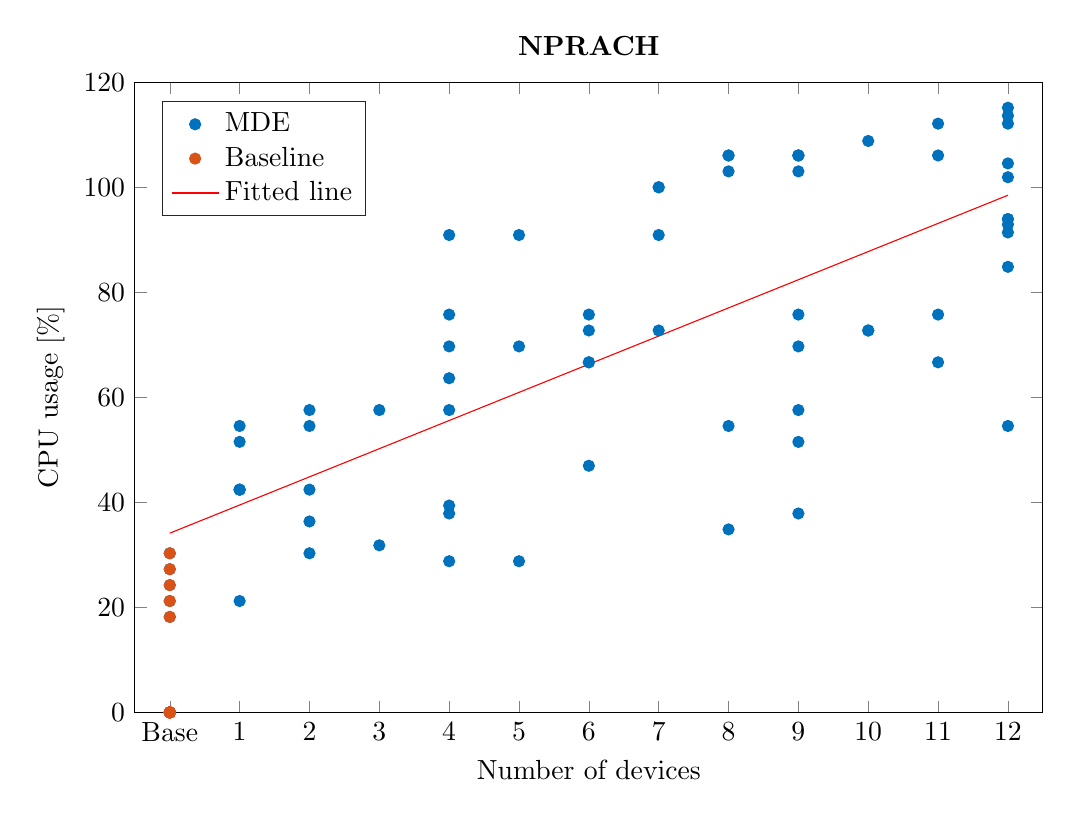
\begin{tikzpicture}

\begin{axis}[%
width=0.951\textwidth,
height=0.66\textwidth,
at={(0\textwidth,0\textwidth)},
scale only axis,
xmin=-0.5,
xmax=12.5,
xtick={0,1,2,3,4,5,6,7,8,9,10,11,12,13,14,15},
xticklabels={{Base},{1},{2},{3},{4},{5},{6},{7},{8},{9},{10},{11},{12},{13},{14},{15}},
xlabel={Number of devices},
ymin=0,
ymax=120,
ylabel={CPU usage [\%]},
axis background/.style={fill=white},
title style={font=\bfseries},
title={NPRACH},
legend style={at={(0.03,0.97)},anchor=north west,legend cell align=left,align=left,draw=white!15!black},
y tick label style={/pgf/number format/fixed}
]
\addplot [color=mycolor1,only marks,mark=*,mark options={solid}]
  table[row sep=crcr]{%
1	42.42\\
8	106.06\\
12	101.915\\
2	30.305\\
12	115.15\\
4	69.7\\
5	90.91\\
6	66.67\\
10	72.73\\
12	113.635\\
2	54.55\\
6	66.67\\
11	66.67\\
12	54.545\\
1	42.42\\
2	36.36\\
3	31.82\\
9	51.515\\
12	92.915\\
3	57.58\\
0	30.3\\
4	37.88\\
9	103.03\\
12	104.545\\
4	28.79\\
6	72.73\\
9	69.7\\
2	42.42\\
8	34.85\\
0	21.21\\
9	106.06\\
4	39.395\\
9	75.76\\
1	21.21\\
7	100\\
10	108.82\\
11	112.12\\
12	84.85\\
5	69.7\\
0	18.18\\
5	28.79\\
7	72.73\\
4	57.58\\
11	106.06\\
12	91.4\\
1	42.42\\
6	46.97\\
8	106.06\\
9	57.575\\
10	72.73\\
12	112.12\\
0	27.27\\
1	54.55\\
9	106.06\\
1	51.52\\
2	57.58\\
4	75.76\\
7	100\\
8	54.545\\
9	37.88\\
0	24.24\\
4	90.91\\
6	75.76\\
9	106.06\\
11	75.76\\
12	93.94\\
4	63.64\\
7	90.91\\
8	103.03\\
12	93.94\\
};
\addlegendentry{MDE};

\addplot [color=mycolor2,only marks,mark=*,mark options={solid}]
  table[row sep=crcr]{%
0	0\\
0	0\\
0	0\\
0	0\\
0	0\\
0	0\\
0	30.3\\
0	0\\
0	0\\
0	21.21\\
0	0\\
0	0\\
0	0\\
0	18.18\\
0	0\\
0	0\\
0	27.27\\
0	0\\
0	24.24\\
0	0\\
};
\addlegendentry{Baseline};

\addplot [color=red,solid]
  table[row sep=crcr]{%
0	34.1310907099265\\
0.012	34.1954441103751\\
0.024	34.2597975108236\\
0.036	34.3241509112722\\
0.048	34.3885043117208\\
0.06	34.4528577121694\\
0.072	34.517211112618\\
0.084	34.5815645130666\\
0.096	34.6459179135152\\
0.108	34.7102713139638\\
0.12	34.7746247144124\\
0.132	34.838978114861\\
0.144	34.9033315153096\\
0.156	34.9676849157582\\
0.168	35.0320383162068\\
0.18	35.0963917166554\\
0.192	35.160745117104\\
0.204	35.2250985175526\\
0.216	35.2894519180011\\
0.228	35.3538053184497\\
0.24	35.4181587188983\\
0.252	35.4825121193469\\
0.264	35.5468655197955\\
0.276	35.6112189202441\\
0.288	35.6755723206927\\
0.3	35.7399257211413\\
0.312	35.8042791215899\\
0.324	35.8686325220385\\
0.336	35.9329859224871\\
0.348	35.9973393229357\\
0.36	36.0616927233843\\
0.372	36.1260461238329\\
0.384	36.1903995242815\\
0.396	36.2547529247301\\
0.408	36.3191063251787\\
0.42	36.3834597256273\\
0.432	36.4478131260758\\
0.444	36.5121665265244\\
0.456	36.576519926973\\
0.468	36.6408733274216\\
0.48	36.7052267278702\\
0.492	36.7695801283188\\
0.504	36.8339335287674\\
0.516	36.898286929216\\
0.528	36.9626403296646\\
0.54	37.0269937301132\\
0.552	37.0913471305618\\
0.564	37.1557005310104\\
0.576	37.220053931459\\
0.588	37.2844073319076\\
0.6	37.3487607323562\\
0.612	37.4131141328048\\
0.624	37.4774675332534\\
0.636	37.5418209337019\\
0.648	37.6061743341505\\
0.66	37.6705277345991\\
0.672	37.7348811350477\\
0.684	37.7992345354963\\
0.696	37.8635879359449\\
0.708	37.9279413363935\\
0.72	37.9922947368421\\
0.732	38.0566481372907\\
0.744	38.1210015377393\\
0.756	38.1853549381879\\
0.768	38.2497083386365\\
0.78	38.3140617390851\\
0.792	38.3784151395337\\
0.804	38.4427685399823\\
0.816	38.5071219404309\\
0.828	38.5714753408795\\
0.84	38.635828741328\\
0.852	38.7001821417766\\
0.864	38.7645355422252\\
0.876	38.8288889426738\\
0.888	38.8932423431224\\
0.9	38.957595743571\\
0.912	39.0219491440196\\
0.924	39.0863025444682\\
0.936	39.1506559449168\\
0.948	39.2150093453654\\
0.96	39.279362745814\\
0.972	39.3437161462626\\
0.984	39.4080695467112\\
0.996	39.4724229471598\\
1.008	39.5367763476084\\
1.02	39.601129748057\\
1.032	39.6654831485056\\
1.044	39.7298365489542\\
1.056	39.7941899494027\\
1.068	39.8585433498513\\
1.08	39.9228967502999\\
1.092	39.9872501507485\\
1.104	40.0516035511971\\
1.116	40.1159569516457\\
1.128	40.1803103520943\\
1.14	40.2446637525429\\
1.152	40.3090171529915\\
1.164	40.3733705534401\\
1.176	40.4377239538887\\
1.188	40.5020773543373\\
1.2	40.5664307547859\\
1.212	40.6307841552345\\
1.224	40.6951375556831\\
1.236	40.7594909561317\\
1.248	40.8238443565803\\
1.26	40.8881977570288\\
1.272	40.9525511574774\\
1.284	41.016904557926\\
1.296	41.0812579583746\\
1.308	41.1456113588232\\
1.32	41.2099647592718\\
1.332	41.2743181597204\\
1.344	41.338671560169\\
1.356	41.4030249606176\\
1.368	41.4673783610662\\
1.38	41.5317317615148\\
1.392	41.5960851619634\\
1.404	41.660438562412\\
1.416	41.7247919628606\\
1.428	41.7891453633092\\
1.44	41.8534987637578\\
1.452	41.9178521642064\\
1.464	41.9822055646549\\
1.476	42.0465589651035\\
1.488	42.1109123655521\\
1.5	42.1752657660007\\
1.512	42.2396191664493\\
1.524	42.3039725668979\\
1.536	42.3683259673465\\
1.548	42.4326793677951\\
1.56	42.4970327682437\\
1.572	42.5613861686923\\
1.584	42.6257395691409\\
1.596	42.6900929695895\\
1.608	42.7544463700381\\
1.62	42.8187997704867\\
1.632	42.8831531709353\\
1.644	42.9475065713839\\
1.656	43.0118599718325\\
1.668	43.076213372281\\
1.68	43.1405667727296\\
1.692	43.2049201731782\\
1.704	43.2692735736268\\
1.716	43.3336269740754\\
1.728	43.397980374524\\
1.74	43.4623337749726\\
1.752	43.5266871754212\\
1.764	43.5910405758698\\
1.776	43.6553939763184\\
1.788	43.719747376767\\
1.8	43.7841007772156\\
1.812	43.8484541776642\\
1.824	43.9128075781128\\
1.836	43.9771609785614\\
1.848	44.04151437901\\
1.86	44.1058677794586\\
1.872	44.1702211799072\\
1.884	44.2345745803557\\
1.896	44.2989279808043\\
1.908	44.3632813812529\\
1.92	44.4276347817015\\
1.932	44.4919881821501\\
1.944	44.5563415825987\\
1.956	44.6206949830473\\
1.968	44.6850483834959\\
1.98	44.7494017839445\\
1.992	44.8137551843931\\
2.004	44.8781085848417\\
2.016	44.9424619852903\\
2.028	45.0068153857389\\
2.04	45.0711687861875\\
2.052	45.1355221866361\\
2.064	45.1998755870847\\
2.076	45.2642289875333\\
2.088	45.3285823879818\\
2.1	45.3929357884304\\
2.112	45.457289188879\\
2.124	45.5216425893276\\
2.136	45.5859959897762\\
2.148	45.6503493902248\\
2.16	45.7147027906734\\
2.172	45.779056191122\\
2.184	45.8434095915706\\
2.196	45.9077629920192\\
2.208	45.9721163924678\\
2.22	46.0364697929164\\
2.232	46.100823193365\\
2.244	46.1651765938136\\
2.256	46.2295299942622\\
2.268	46.2938833947108\\
2.28	46.3582367951594\\
2.292	46.422590195608\\
2.304	46.4869435960565\\
2.316	46.5512969965051\\
2.328	46.6156503969537\\
2.34	46.6800037974023\\
2.352	46.7443571978509\\
2.364	46.8087105982995\\
2.376	46.8730639987481\\
2.388	46.9374173991967\\
2.4	47.0017707996453\\
2.412	47.0661242000939\\
2.424	47.1304776005425\\
2.436	47.1948310009911\\
2.448	47.2591844014397\\
2.46	47.3235378018883\\
2.472	47.3878912023369\\
2.484	47.4522446027855\\
2.496	47.5165980032341\\
2.508	47.5809514036826\\
2.52	47.6453048041312\\
2.532	47.7096582045798\\
2.544	47.7740116050284\\
2.556	47.838365005477\\
2.568	47.9027184059256\\
2.58	47.9670718063742\\
2.592	48.0314252068228\\
2.604	48.0957786072714\\
2.616	48.16013200772\\
2.628	48.2244854081686\\
2.64	48.2888388086172\\
2.652	48.3531922090658\\
2.664	48.4175456095144\\
2.676	48.481899009963\\
2.688	48.5462524104116\\
2.7	48.6106058108602\\
2.712	48.6749592113087\\
2.724	48.7393126117573\\
2.736	48.8036660122059\\
2.748	48.8680194126545\\
2.76	48.9323728131031\\
2.772	48.9967262135517\\
2.784	49.0610796140003\\
2.796	49.1254330144489\\
2.808	49.1897864148975\\
2.82	49.2541398153461\\
2.832	49.3184932157947\\
2.844	49.3828466162433\\
2.856	49.4472000166919\\
2.868	49.5115534171405\\
2.88	49.5759068175891\\
2.892	49.6402602180377\\
2.904	49.7046136184862\\
2.916	49.7689670189348\\
2.928	49.8333204193834\\
2.94	49.897673819832\\
2.952	49.9620272202806\\
2.964	50.0263806207292\\
2.976	50.0907340211778\\
2.988	50.1550874216264\\
3	50.219440822075\\
3.012	50.2837942225236\\
3.024	50.3481476229722\\
3.036	50.4125010234208\\
3.048	50.4768544238694\\
3.06	50.541207824318\\
3.072	50.6055612247666\\
3.084	50.6699146252152\\
3.096	50.7342680256638\\
3.108	50.7986214261124\\
3.12	50.862974826561\\
3.132	50.9273282270095\\
3.144	50.9916816274581\\
3.156	51.0560350279067\\
3.168	51.1203884283553\\
3.18	51.1847418288039\\
3.192	51.2490952292525\\
3.204	51.3134486297011\\
3.216	51.3778020301497\\
3.228	51.4421554305983\\
3.24	51.5065088310469\\
3.252	51.5708622314955\\
3.264	51.6352156319441\\
3.276	51.6995690323927\\
3.288	51.7639224328413\\
3.3	51.8282758332899\\
3.312	51.8926292337385\\
3.324	51.9569826341871\\
3.336	52.0213360346356\\
3.348	52.0856894350842\\
3.36	52.1500428355328\\
3.372	52.2143962359814\\
3.384	52.27874963643\\
3.396	52.3431030368786\\
3.408	52.4074564373272\\
3.42	52.4718098377758\\
3.432	52.5361632382244\\
3.444	52.600516638673\\
3.456	52.6648700391216\\
3.468	52.7292234395702\\
3.48	52.7935768400188\\
3.492	52.8579302404674\\
3.504	52.922283640916\\
3.516	52.9866370413646\\
3.528	53.0509904418132\\
3.54	53.1153438422618\\
3.552	53.1796972427103\\
3.564	53.2440506431589\\
3.576	53.3084040436075\\
3.588	53.3727574440561\\
3.6	53.4371108445047\\
3.612	53.5014642449533\\
3.624	53.5658176454019\\
3.636	53.6301710458505\\
3.648	53.6945244462991\\
3.66	53.7588778467477\\
3.672	53.8232312471963\\
3.684	53.8875846476449\\
3.696	53.9519380480935\\
3.708	54.0162914485421\\
3.72	54.0806448489907\\
3.732	54.1449982494393\\
3.744	54.2093516498879\\
3.756	54.2737050503364\\
3.768	54.338058450785\\
3.78	54.4024118512336\\
3.792	54.4667652516822\\
3.804	54.5311186521308\\
3.816	54.5954720525794\\
3.828	54.659825453028\\
3.84	54.7241788534766\\
3.852	54.7885322539252\\
3.864	54.8528856543738\\
3.876	54.9172390548224\\
3.888	54.981592455271\\
3.9	55.0459458557196\\
3.912	55.1102992561682\\
3.924	55.1746526566168\\
3.936	55.2390060570654\\
3.948	55.3033594575139\\
3.96	55.3677128579625\\
3.972	55.4320662584111\\
3.984	55.4964196588597\\
3.996	55.5607730593083\\
4.008	55.6251264597569\\
4.02	55.6894798602055\\
4.032	55.7538332606541\\
4.044	55.8181866611027\\
4.056	55.8825400615513\\
4.068	55.9468934619999\\
4.08	56.0112468624485\\
4.092	56.0756002628971\\
4.104	56.1399536633457\\
4.116	56.2043070637943\\
4.128	56.2686604642429\\
4.14	56.3330138646915\\
4.152	56.39736726514\\
4.164	56.4617206655886\\
4.176	56.5260740660372\\
4.188	56.5904274664858\\
4.2	56.6547808669344\\
4.212	56.719134267383\\
4.224	56.7834876678316\\
4.236	56.8478410682802\\
4.248	56.9121944687288\\
4.26	56.9765478691774\\
4.272	57.040901269626\\
4.284	57.1052546700746\\
4.296	57.1696080705232\\
4.308	57.2339614709718\\
4.32	57.2983148714204\\
4.332	57.362668271869\\
4.344	57.4270216723176\\
4.356	57.4913750727662\\
4.368	57.5557284732147\\
4.38	57.6200818736633\\
4.392	57.6844352741119\\
4.404	57.7487886745605\\
4.416	57.8131420750091\\
4.428	57.8774954754577\\
4.44	57.9418488759063\\
4.452	58.0062022763549\\
4.464	58.0705556768035\\
4.476	58.1349090772521\\
4.488	58.1992624777007\\
4.5	58.2636158781493\\
4.512	58.3279692785979\\
4.524	58.3923226790465\\
4.536	58.4566760794951\\
4.548	58.5210294799437\\
4.56	58.5853828803923\\
4.572	58.6497362808408\\
4.584	58.7140896812894\\
4.596	58.778443081738\\
4.608	58.8427964821866\\
4.62	58.9071498826352\\
4.632	58.9715032830838\\
4.644	59.0358566835324\\
4.656	59.100210083981\\
4.668	59.1645634844296\\
4.68	59.2289168848782\\
4.692	59.2932702853268\\
4.704	59.3576236857754\\
4.716	59.421977086224\\
4.728	59.4863304866726\\
4.74	59.5506838871212\\
4.752	59.6150372875698\\
4.764	59.6793906880184\\
4.776	59.743744088467\\
4.788	59.8080974889156\\
4.8	59.8724508893641\\
4.812	59.9368042898127\\
4.824	60.0011576902613\\
4.836	60.0655110907099\\
4.848	60.1298644911585\\
4.86	60.1942178916071\\
4.872	60.2585712920557\\
4.884	60.3229246925043\\
4.896	60.3872780929529\\
4.908	60.4516314934015\\
4.92	60.5159848938501\\
4.932	60.5803382942987\\
4.944	60.6446916947473\\
4.956	60.7090450951959\\
4.968	60.7733984956445\\
4.98	60.8377518960931\\
4.992	60.9021052965416\\
5.004	60.9664586969902\\
5.016	61.0308120974388\\
5.028	61.0951654978874\\
5.04	61.159518898336\\
5.052	61.2238722987846\\
5.064	61.2882256992332\\
5.076	61.3525790996818\\
5.088	61.4169325001304\\
5.1	61.481285900579\\
5.112	61.5456393010276\\
5.124	61.6099927014762\\
5.136	61.6743461019248\\
5.148	61.7386995023734\\
5.16	61.803052902822\\
5.172	61.8674063032706\\
5.184	61.9317597037192\\
5.196	61.9961131041677\\
5.208	62.0604665046163\\
5.22	62.1248199050649\\
5.232	62.1891733055135\\
5.244	62.2535267059621\\
5.256	62.3178801064107\\
5.268	62.3822335068593\\
5.28	62.4465869073079\\
5.292	62.5109403077565\\
5.304	62.5752937082051\\
5.316	62.6396471086537\\
5.328	62.7040005091023\\
5.34	62.7683539095509\\
5.352	62.8327073099995\\
5.364	62.8970607104481\\
5.376	62.9614141108967\\
5.388	63.0257675113453\\
5.4	63.0901209117938\\
5.412	63.1544743122424\\
5.424	63.218827712691\\
5.436	63.2831811131396\\
5.448	63.3475345135882\\
5.46	63.4118879140368\\
5.472	63.4762413144854\\
5.484	63.540594714934\\
5.496	63.6049481153826\\
5.508	63.6693015158312\\
5.52	63.7336549162798\\
5.532	63.7980083167284\\
5.544	63.862361717177\\
5.556	63.9267151176256\\
5.568	63.9910685180742\\
5.58	64.0554219185228\\
5.592	64.1197753189714\\
5.604	64.18412871942\\
5.616	64.2484821198686\\
5.628	64.3128355203171\\
5.64	64.3771889207657\\
5.652	64.4415423212143\\
5.664	64.5058957216629\\
5.676	64.5702491221115\\
5.688	64.6346025225601\\
5.7	64.6989559230087\\
5.712	64.7633093234573\\
5.724	64.8276627239059\\
5.736	64.8920161243545\\
5.748	64.9563695248031\\
5.76	65.0207229252517\\
5.772	65.0850763257003\\
5.784	65.1494297261489\\
5.796	65.2137831265975\\
5.808	65.2781365270461\\
5.82	65.3424899274947\\
5.832	65.4068433279432\\
5.844	65.4711967283918\\
5.856	65.5355501288404\\
5.868	65.599903529289\\
5.88	65.6642569297376\\
5.892	65.7286103301862\\
5.904	65.7929637306348\\
5.916	65.8573171310834\\
5.928	65.921670531532\\
5.94	65.9860239319806\\
5.952	66.0503773324292\\
5.964	66.1147307328778\\
5.976	66.1790841333264\\
5.988	66.243437533775\\
6	66.3077909342236\\
6.012	66.3721443346722\\
6.024	66.4364977351208\\
6.036	66.5008511355693\\
6.048	66.5652045360179\\
6.06	66.6295579364665\\
6.072	66.6939113369151\\
6.084	66.7582647373637\\
6.096	66.8226181378123\\
6.108	66.8869715382609\\
6.12	66.9513249387095\\
6.132	67.0156783391581\\
6.144	67.0800317396067\\
6.156	67.1443851400553\\
6.168	67.2087385405039\\
6.18	67.2730919409525\\
6.192	67.3374453414011\\
6.204	67.4017987418497\\
6.216	67.4661521422983\\
6.228	67.5305055427469\\
6.24	67.5948589431954\\
6.252	67.659212343644\\
6.264	67.7235657440926\\
6.276	67.7879191445412\\
6.288	67.8522725449898\\
6.3	67.9166259454384\\
6.312	67.980979345887\\
6.324	68.0453327463356\\
6.336	68.1096861467842\\
6.348	68.1740395472328\\
6.36	68.2383929476814\\
6.372	68.30274634813\\
6.384	68.3670997485786\\
6.396	68.4314531490272\\
6.408	68.4958065494758\\
6.42	68.5601599499244\\
6.432	68.624513350373\\
6.444	68.6888667508215\\
6.456	68.7532201512701\\
6.468	68.8175735517187\\
6.48	68.8819269521673\\
6.492	68.9462803526159\\
6.504	69.0106337530645\\
6.516	69.0749871535131\\
6.528	69.1393405539617\\
6.54	69.2036939544103\\
6.552	69.2680473548589\\
6.564	69.3324007553075\\
6.576	69.3967541557561\\
6.588	69.4611075562047\\
6.6	69.5254609566533\\
6.612	69.5898143571019\\
6.624	69.6541677575505\\
6.636	69.718521157999\\
6.648	69.7828745584476\\
6.66	69.8472279588962\\
6.672	69.9115813593448\\
6.684	69.9759347597934\\
6.696	70.040288160242\\
6.708	70.1046415606906\\
6.72	70.1689949611392\\
6.732	70.2333483615878\\
6.744	70.2977017620364\\
6.756	70.362055162485\\
6.768	70.4264085629336\\
6.78	70.4907619633822\\
6.792	70.5551153638308\\
6.804	70.6194687642794\\
6.816	70.683822164728\\
6.828	70.7481755651766\\
6.84	70.8125289656251\\
6.852	70.8768823660737\\
6.864	70.9412357665223\\
6.876	71.0055891669709\\
6.888	71.0699425674195\\
6.9	71.1342959678681\\
6.912	71.1986493683167\\
6.924	71.2630027687653\\
6.936	71.3273561692139\\
6.948	71.3917095696625\\
6.96	71.4560629701111\\
6.972	71.5204163705597\\
6.984	71.5847697710083\\
6.996	71.6491231714569\\
7.008	71.7134765719055\\
7.02	71.7778299723541\\
7.032	71.8421833728027\\
7.044	71.9065367732513\\
7.056	71.9708901736998\\
7.068	72.0352435741484\\
7.08	72.099596974597\\
7.092	72.1639503750456\\
7.104	72.2283037754942\\
7.116	72.2926571759428\\
7.128	72.3570105763914\\
7.14	72.42136397684\\
7.152	72.4857173772886\\
7.164	72.5500707777372\\
7.176	72.6144241781858\\
7.188	72.6787775786344\\
7.2	72.743130979083\\
7.212	72.8074843795316\\
7.224	72.8718377799802\\
7.236	72.9361911804288\\
7.248	73.0005445808774\\
7.26	73.0648979813259\\
7.272	73.1292513817745\\
7.284	73.1936047822231\\
7.296	73.2579581826717\\
7.308	73.3223115831203\\
7.32	73.3866649835689\\
7.332	73.4510183840175\\
7.344	73.5153717844661\\
7.356	73.5797251849147\\
7.368	73.6440785853633\\
7.38	73.7084319858119\\
7.392	73.7727853862605\\
7.404	73.8371387867091\\
7.416	73.9014921871577\\
7.428	73.9658455876063\\
7.44	74.0301989880549\\
7.452	74.0945523885035\\
7.464	74.1589057889521\\
7.476	74.2232591894007\\
7.488	74.2876125898492\\
7.5	74.3519659902978\\
7.512	74.4163193907464\\
7.524	74.480672791195\\
7.536	74.5450261916436\\
7.548	74.6093795920922\\
7.56	74.6737329925408\\
7.572	74.7380863929894\\
7.584	74.802439793438\\
7.596	74.8667931938866\\
7.608	74.9311465943352\\
7.62	74.9954999947838\\
7.632	75.0598533952324\\
7.644	75.124206795681\\
7.656	75.1885601961296\\
7.668	75.2529135965782\\
7.68	75.3172669970267\\
7.692	75.3816203974753\\
7.704	75.4459737979239\\
7.716	75.5103271983725\\
7.728	75.5746805988211\\
7.74	75.6390339992697\\
7.752	75.7033873997183\\
7.764	75.7677408001669\\
7.776	75.8320942006155\\
7.788	75.8964476010641\\
7.8	75.9608010015127\\
7.812	76.0251544019613\\
7.824	76.0895078024099\\
7.836	76.1538612028585\\
7.848	76.2182146033071\\
7.86	76.2825680037557\\
7.872	76.3469214042043\\
7.884	76.4112748046529\\
7.896	76.4756282051014\\
7.908	76.53998160555\\
7.92	76.6043350059986\\
7.932	76.6686884064472\\
7.944	76.7330418068958\\
7.956	76.7973952073444\\
7.968	76.861748607793\\
7.98	76.9261020082416\\
7.992	76.9904554086902\\
8.004	77.0548088091388\\
8.016	77.1191622095874\\
8.028	77.183515610036\\
8.04	77.2478690104846\\
8.052	77.3122224109332\\
8.064	77.3765758113818\\
8.076	77.4409292118304\\
8.088	77.505282612279\\
8.1	77.5696360127275\\
8.112	77.6339894131761\\
8.124	77.6983428136247\\
8.136	77.7626962140733\\
8.148	77.8270496145219\\
8.16	77.8914030149705\\
8.172	77.9557564154191\\
8.184	78.0201098158677\\
8.196	78.0844632163163\\
8.208	78.1488166167649\\
8.22	78.2131700172135\\
8.232	78.2775234176621\\
8.244	78.3418768181107\\
8.256	78.4062302185593\\
8.268	78.4705836190079\\
8.28	78.5349370194565\\
8.292	78.5992904199051\\
8.304	78.6636438203537\\
8.316	78.7279972208023\\
8.328	78.7923506212508\\
8.34	78.8567040216994\\
8.352	78.921057422148\\
8.364	78.9854108225966\\
8.376	79.0497642230452\\
8.388	79.1141176234938\\
8.4	79.1784710239424\\
8.412	79.242824424391\\
8.424	79.3071778248396\\
8.436	79.3715312252882\\
8.448	79.4358846257368\\
8.46	79.5002380261854\\
8.472	79.564591426634\\
8.484	79.6289448270826\\
8.496	79.6932982275312\\
8.508	79.7576516279798\\
8.52	79.8220050284284\\
8.532	79.8863584288769\\
8.544	79.9507118293255\\
8.556	80.0150652297741\\
8.568	80.0794186302227\\
8.58	80.1437720306713\\
8.592	80.2081254311199\\
8.604	80.2724788315685\\
8.616	80.3368322320171\\
8.628	80.4011856324657\\
8.64	80.4655390329143\\
8.652	80.5298924333629\\
8.664	80.5942458338115\\
8.676	80.6585992342601\\
8.688	80.7229526347087\\
8.7	80.7873060351573\\
8.712	80.8516594356059\\
8.724	80.9160128360544\\
8.736	80.980366236503\\
8.748	81.0447196369516\\
8.76	81.1090730374002\\
8.772	81.1734264378488\\
8.784	81.2377798382974\\
8.796	81.302133238746\\
8.808	81.3664866391946\\
8.82	81.4308400396432\\
8.832	81.4951934400918\\
8.844	81.5595468405404\\
8.856	81.623900240989\\
8.868	81.6882536414376\\
8.88	81.7526070418862\\
8.892	81.8169604423348\\
8.904	81.8813138427834\\
8.916	81.945667243232\\
8.928	82.0100206436805\\
8.94	82.0743740441291\\
8.952	82.1387274445777\\
8.964	82.2030808450263\\
8.976	82.2674342454749\\
8.988	82.3317876459235\\
9	82.3961410463721\\
9.012	82.4604944468207\\
9.024	82.5248478472693\\
9.036	82.5892012477179\\
9.048	82.6535546481665\\
9.06	82.7179080486151\\
9.072	82.7822614490637\\
9.084	82.8466148495123\\
9.096	82.9109682499609\\
9.108	82.9753216504095\\
9.12	83.0396750508581\\
9.132	83.1040284513066\\
9.144	83.1683818517552\\
9.156	83.2327352522038\\
9.168	83.2970886526524\\
9.18	83.361442053101\\
9.192	83.4257954535496\\
9.204	83.4901488539982\\
9.216	83.5545022544468\\
9.228	83.6188556548954\\
9.24	83.683209055344\\
9.252	83.7475624557926\\
9.264	83.8119158562412\\
9.276	83.8762692566898\\
9.288	83.9406226571384\\
9.3	84.004976057587\\
9.312	84.0693294580356\\
9.324	84.1336828584842\\
9.336	84.1980362589327\\
9.348	84.2623896593813\\
9.36	84.3267430598299\\
9.372	84.3910964602785\\
9.384	84.4554498607271\\
9.396	84.5198032611757\\
9.408	84.5841566616243\\
9.42	84.6485100620729\\
9.432	84.7128634625215\\
9.444	84.7772168629701\\
9.456	84.8415702634187\\
9.468	84.9059236638673\\
9.48	84.9702770643159\\
9.492	85.0346304647645\\
9.504	85.0989838652131\\
9.516	85.1633372656617\\
9.528	85.2276906661103\\
9.54	85.2920440665589\\
9.552	85.3563974670074\\
9.564	85.420750867456\\
9.576	85.4851042679046\\
9.588	85.5494576683532\\
9.6	85.6138110688018\\
9.612	85.6781644692504\\
9.624	85.742517869699\\
9.636	85.8068712701476\\
9.648	85.8712246705962\\
9.66	85.9355780710448\\
9.672	85.9999314714934\\
9.684	86.064284871942\\
9.696	86.1286382723906\\
9.708	86.1929916728392\\
9.72	86.2573450732878\\
9.732	86.3216984737363\\
9.744	86.3860518741849\\
9.756	86.4504052746335\\
9.768	86.5147586750821\\
9.78	86.5791120755307\\
9.792	86.6434654759793\\
9.804	86.7078188764279\\
9.816	86.7721722768765\\
9.828	86.8365256773251\\
9.84	86.9008790777737\\
9.852	86.9652324782223\\
9.864	87.0295858786709\\
9.876	87.0939392791195\\
9.888	87.1582926795681\\
9.9	87.2226460800167\\
9.912	87.2869994804653\\
9.924	87.3513528809139\\
9.936	87.4157062813625\\
9.948	87.4800596818111\\
9.96	87.5444130822597\\
9.972	87.6087664827082\\
9.984	87.6731198831568\\
9.996	87.7374732836054\\
10.008	87.801826684054\\
10.02	87.8661800845026\\
10.032	87.9305334849512\\
10.044	87.9948868853998\\
10.056	88.0592402858484\\
10.068	88.123593686297\\
10.08	88.1879470867456\\
10.092	88.2523004871942\\
10.104	88.3166538876428\\
10.116	88.3810072880914\\
10.128	88.44536068854\\
10.14	88.5097140889886\\
10.152	88.5740674894372\\
10.164	88.6384208898858\\
10.176	88.7027742903343\\
10.188	88.7671276907829\\
10.2	88.8314810912315\\
10.212	88.8958344916801\\
10.224	88.9601878921287\\
10.236	89.0245412925773\\
10.248	89.0888946930259\\
10.26	89.1532480934745\\
10.272	89.2176014939231\\
10.284	89.2819548943717\\
10.296	89.3463082948203\\
10.308	89.4106616952689\\
10.32	89.4750150957175\\
10.332	89.5393684961661\\
10.344	89.6037218966147\\
10.356	89.6680752970633\\
10.368	89.7324286975119\\
10.38	89.7967820979605\\
10.392	89.861135498409\\
10.404	89.9254888988576\\
10.416	89.9898422993062\\
10.428	90.0541956997548\\
10.44	90.1185491002034\\
10.452	90.182902500652\\
10.464	90.2472559011006\\
10.476	90.3116093015492\\
10.488	90.3759627019978\\
10.5	90.4403161024464\\
10.512	90.504669502895\\
10.524	90.5690229033436\\
10.536	90.6333763037922\\
10.548	90.6977297042408\\
10.56	90.7620831046894\\
10.572	90.826436505138\\
10.584	90.8907899055865\\
10.596	90.9551433060351\\
10.608	91.0194967064838\\
10.62	91.0838501069323\\
10.632	91.1482035073809\\
10.644	91.2125569078295\\
10.656	91.2769103082781\\
10.668	91.3412637087267\\
10.68	91.4056171091753\\
10.692	91.4699705096239\\
10.704	91.5343239100725\\
10.716	91.5986773105211\\
10.728	91.6630307109697\\
10.74	91.7273841114183\\
10.752	91.7917375118669\\
10.764	91.8560909123155\\
10.776	91.9204443127641\\
10.788	91.9847977132127\\
10.8	92.0491511136613\\
10.812	92.1135045141098\\
10.824	92.1778579145584\\
10.836	92.242211315007\\
10.848	92.3065647154556\\
10.86	92.3709181159042\\
10.872	92.4352715163528\\
10.884	92.4996249168014\\
10.896	92.56397831725\\
10.908	92.6283317176986\\
10.92	92.6926851181472\\
10.932	92.7570385185958\\
10.944	92.8213919190444\\
10.956	92.885745319493\\
10.968	92.9500987199416\\
10.98	93.0144521203902\\
10.992	93.0788055208388\\
11.004	93.1431589212874\\
11.016	93.2075123217359\\
11.028	93.2718657221845\\
11.04	93.3362191226331\\
11.052	93.4005725230817\\
11.064	93.4649259235303\\
11.076	93.5292793239789\\
11.088	93.5936327244275\\
11.1	93.6579861248761\\
11.112	93.7223395253247\\
11.124	93.7866929257733\\
11.136	93.8510463262219\\
11.148	93.9153997266705\\
11.16	93.9797531271191\\
11.172	94.0441065275677\\
11.184	94.1084599280163\\
11.196	94.1728133284649\\
11.208	94.2371667289135\\
11.22	94.301520129362\\
11.232	94.3658735298106\\
11.244	94.4302269302592\\
11.256	94.4945803307078\\
11.268	94.5589337311564\\
11.28	94.623287131605\\
11.292	94.6876405320536\\
11.304	94.7519939325022\\
11.316	94.8163473329508\\
11.328	94.8807007333994\\
11.34	94.945054133848\\
11.352	95.0094075342966\\
11.364	95.0737609347452\\
11.376	95.1381143351938\\
11.388	95.2024677356424\\
11.4	95.266821136091\\
11.412	95.3311745365396\\
11.424	95.3955279369881\\
11.436	95.4598813374367\\
11.448	95.5242347378853\\
11.46	95.5885881383339\\
11.472	95.6529415387825\\
11.484	95.7172949392311\\
11.496	95.7816483396797\\
11.508	95.8460017401283\\
11.52	95.9103551405769\\
11.532	95.9747085410255\\
11.544	96.0390619414741\\
11.556	96.1034153419227\\
11.568	96.1677687423713\\
11.58	96.2321221428199\\
11.592	96.2964755432685\\
11.604	96.3608289437171\\
11.616	96.4251823441656\\
11.628	96.4895357446142\\
11.64	96.5538891450628\\
11.652	96.6182425455114\\
11.664	96.68259594596\\
11.676	96.7469493464086\\
11.688	96.8113027468572\\
11.7	96.8756561473058\\
11.712	96.9400095477544\\
11.724	97.004362948203\\
11.736	97.0687163486516\\
11.748	97.1330697491002\\
11.76	97.1974231495488\\
11.772	97.2617765499974\\
11.784	97.326129950446\\
11.796	97.3904833508946\\
11.808	97.4548367513432\\
11.82	97.5191901517917\\
11.832	97.5835435522403\\
11.844	97.6478969526889\\
11.856	97.7122503531375\\
11.868	97.7766037535861\\
11.88	97.8409571540347\\
11.892	97.9053105544833\\
11.904	97.9696639549319\\
11.916	98.0340173553805\\
11.928	98.0983707558291\\
11.94	98.1627241562777\\
11.952	98.2270775567263\\
11.964	98.2914309571749\\
11.976	98.3557843576235\\
11.988	98.4201377580721\\
12	98.4844911585207\\
};
\addlegendentry{Fitted line};

\end{axis}
\end{tikzpicture}%}
\caption{CPU usage for the NPRACH step of the MDE for different number of devices and the baseline emulator. The fitted line is a linear approximation}
\label{fig:CPU_NPRACH}
\end{figure}

The fitted line for the CPU usage is estimated to be:
\begin{equation}
CPU_{NPRACH} = 5.36 \cdot NoD + 34.13
\end{equation}

As seen on \autoref{fig:CPU_NPRACH}, the tendency is similar to the other steps. As the NPRACH step is even shorter in time than the NB-SIB2 step (1-2 samples), the spread is even wider than at the previous step.

\subsection{Summary}
At all steps in the process CPU usage rises with the number of devices, meaning the maximum number of devices the system can support can be found, when the system hits full usage. In \autoref{tab:NoDCPU} the maximum supported number of devices for each step can be seen. The number is calculated from the linear approximation, shown in all the plot throughout this section.

\begin{table}[H]
\centering
\begin{tabular}{|c|c|c|}
\hline
Steps & CPU kernels & NoD \\
\hline
Initialization & 1 & 27 \\
\hline
Synchronization & 1 & 43 \\
\hline
Decoding of MIB-NB & 1 & 73 \\
\hline
SIB1 & 1 & 67 \\
\hline
SIB2 & 1 & 112 \\
\hline
NPRACH & 1 & 124 \\
\hline
\end{tabular}
\caption{Number of devices to hit full CPU usage for the different steps.}
\label{tab:NoDCPU}
\end{table}

\section{Memory usage}
To test the memory usage, the massive emulator is run once for each number of devices, as well for the baseline emulator. As all the buffers and bigger arrays reserve space in the memory in the initialization step, the amount of memory use does not change during the emulation or between two emulations. It does change compared to number of devices, as this effects directly the amount of buffers and arrays that should be allocated. The results can be seen on \autoref{fig:RAMusage}.

\begin{figure}[H]
\tikzsetnextfilename{RAMusage}
\centering
\resizebox{0.5\textwidth}{!}{
% This file was created by matlab2tikz.
%
%The latest updates can be retrieved from
%  http://www.mathworks.com/matlabcentral/fileexchange/22022-matlab2tikz-matlab2tikz
%where you can also make suggestions and rate matlab2tikz.
%
%total RAM size = 32845968 KiB
%
\definecolor{mycolor1}{rgb}{0.00000,0.44700,0.74100}%
\definecolor{mycolor2}{rgb}{0.85000,0.32500,0.09800}%
%
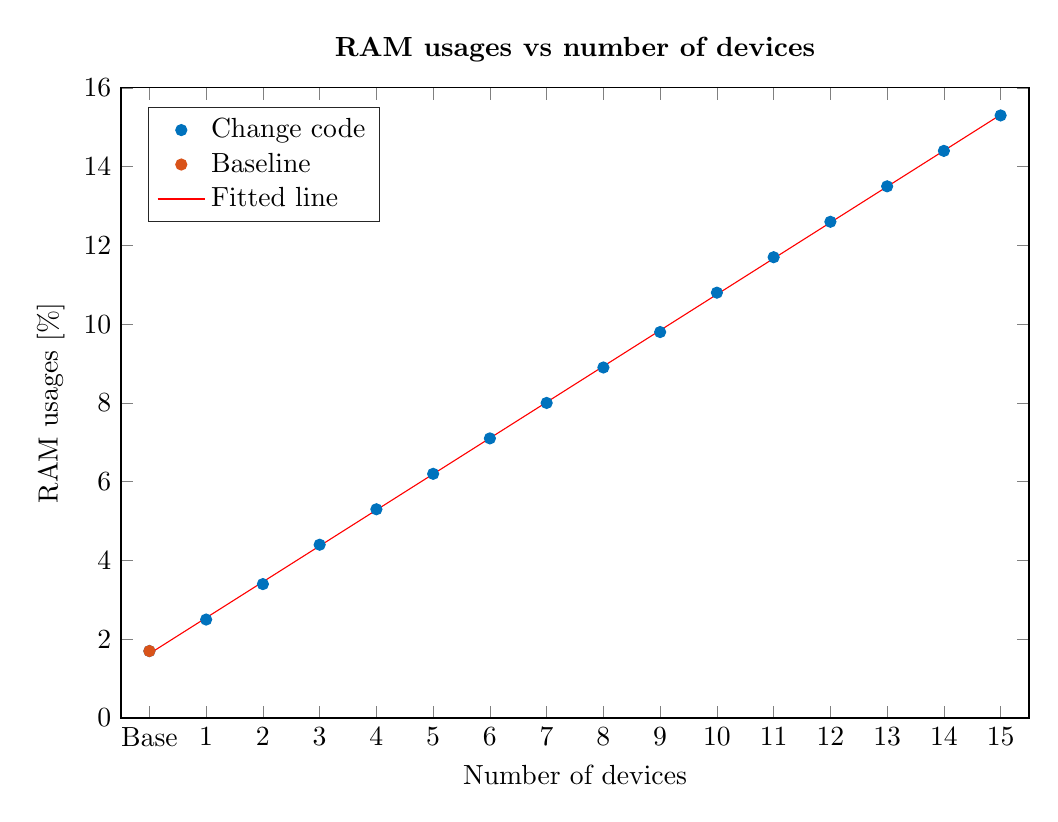
\begin{tikzpicture}

\begin{axis}[%
width=0.951\textwidth,
height=0.66\textwidth,
at={(0\textwidth,0\textwidth)},
scale only axis,
xmin=-0.5,
xmax=15.5,
xtick={0,1,2,3,4,5,6,7,8,9,10,11,12,13,14,15},
xticklabels={{Base},{1},{2},{3},{4},{5},{6},{7},{8},{9},{10},{11},{12},{13},{14},{15}},
xlabel={Number of devices},
ymin=0,
ymax=16,
ylabel={RAM usages [\%]},
axis background/.style={fill=white},
title style={font=\bfseries},
title={RAM usages vs number of devices},
legend style={at={(0.03,0.97)},anchor=north west,legend cell align=left,align=left,draw=white!15!black},
y tick label style={/pgf/number format/fixed}
]
\addplot [color=mycolor1,only marks,mark=*,mark options={solid}]
  table[row sep=crcr]{%
0	1.7\\
1	2.5\\
2	3.4\\
3	4.4\\
4	5.3\\
5	6.2\\
6	7.1\\
7	8\\
8	8.9\\
9	9.8\\
10	10.8\\
11	11.7\\
12	12.6\\
13	13.5\\
14	14.4\\
15	15.3\\
};
\addlegendentry{Change code};

\addplot [color=mycolor2,only marks,mark=*,mark options={solid}]
  table[row sep=crcr]{%
0	1.7\\
};
\addlegendentry{Baseline};

\addplot [color=red,solid]
  table[row sep=crcr]{%
0	1.63235294117647\\
0.015	1.64603823529412\\
0.03	1.65972352941176\\
0.045	1.67340882352941\\
0.06	1.68709411764706\\
0.075	1.70077941176471\\
0.09	1.71446470588235\\
0.105	1.72815\\
0.12	1.74183529411765\\
0.135	1.75552058823529\\
0.15	1.76920588235294\\
0.165	1.78289117647059\\
0.18	1.79657647058824\\
0.195	1.81026176470588\\
0.21	1.82394705882353\\
0.225	1.83763235294118\\
0.24	1.85131764705882\\
0.255	1.86500294117647\\
0.27	1.87868823529412\\
0.285	1.89237352941176\\
0.3	1.90605882352941\\
0.315	1.91974411764706\\
0.33	1.93342941176471\\
0.345	1.94711470588235\\
0.36	1.9608\\
0.375	1.97448529411765\\
0.39	1.98817058823529\\
0.405	2.00185588235294\\
0.42	2.01554117647059\\
0.435	2.02922647058824\\
0.45	2.04291176470588\\
0.465	2.05659705882353\\
0.48	2.07028235294118\\
0.495	2.08396764705882\\
0.51	2.09765294117647\\
0.525	2.11133823529412\\
0.54	2.12502352941176\\
0.555	2.13870882352941\\
0.57	2.15239411764706\\
0.585	2.16607941176471\\
0.6	2.17976470588235\\
0.615	2.19345\\
0.63	2.20713529411765\\
0.645	2.22082058823529\\
0.66	2.23450588235294\\
0.675	2.24819117647059\\
0.69	2.26187647058824\\
0.705	2.27556176470588\\
0.72	2.28924705882353\\
0.735	2.30293235294118\\
0.75	2.31661764705882\\
0.765	2.33030294117647\\
0.78	2.34398823529412\\
0.795	2.35767352941176\\
0.81	2.37135882352941\\
0.825	2.38504411764706\\
0.84	2.39872941176471\\
0.855	2.41241470588235\\
0.87	2.4261\\
0.885	2.43978529411765\\
0.9	2.45347058823529\\
0.915	2.46715588235294\\
0.93	2.48084117647059\\
0.945	2.49452647058824\\
0.96	2.50821176470588\\
0.975	2.52189705882353\\
0.99	2.53558235294118\\
1.005	2.54926764705882\\
1.02	2.56295294117647\\
1.035	2.57663823529412\\
1.05	2.59032352941176\\
1.065	2.60400882352941\\
1.08	2.61769411764706\\
1.095	2.63137941176471\\
1.11	2.64506470588235\\
1.125	2.65875\\
1.14	2.67243529411765\\
1.155	2.68612058823529\\
1.17	2.69980588235294\\
1.185	2.71349117647059\\
1.2	2.72717647058824\\
1.215	2.74086176470588\\
1.23	2.75454705882353\\
1.245	2.76823235294118\\
1.26	2.78191764705882\\
1.275	2.79560294117647\\
1.29	2.80928823529412\\
1.305	2.82297352941176\\
1.32	2.83665882352941\\
1.335	2.85034411764706\\
1.35	2.86402941176471\\
1.365	2.87771470588235\\
1.38	2.8914\\
1.395	2.90508529411765\\
1.41	2.91877058823529\\
1.425	2.93245588235294\\
1.44	2.94614117647059\\
1.455	2.95982647058824\\
1.47	2.97351176470588\\
1.485	2.98719705882353\\
1.5	3.00088235294118\\
1.515	3.01456764705882\\
1.53	3.02825294117647\\
1.545	3.04193823529412\\
1.56	3.05562352941176\\
1.575	3.06930882352941\\
1.59	3.08299411764706\\
1.605	3.09667941176471\\
1.62	3.11036470588235\\
1.635	3.12405\\
1.65	3.13773529411765\\
1.665	3.15142058823529\\
1.68	3.16510588235294\\
1.695	3.17879117647059\\
1.71	3.19247647058824\\
1.725	3.20616176470588\\
1.74	3.21984705882353\\
1.755	3.23353235294118\\
1.77	3.24721764705882\\
1.785	3.26090294117647\\
1.8	3.27458823529412\\
1.815	3.28827352941176\\
1.83	3.30195882352941\\
1.845	3.31564411764706\\
1.86	3.32932941176471\\
1.875	3.34301470588235\\
1.89	3.3567\\
1.905	3.37038529411765\\
1.92	3.38407058823529\\
1.935	3.39775588235294\\
1.95	3.41144117647059\\
1.965	3.42512647058824\\
1.98	3.43881176470588\\
1.995	3.45249705882353\\
2.01	3.46618235294118\\
2.025	3.47986764705882\\
2.04	3.49355294117647\\
2.055	3.50723823529412\\
2.07	3.52092352941176\\
2.085	3.53460882352941\\
2.1	3.54829411764706\\
2.115	3.56197941176471\\
2.13	3.57566470588235\\
2.145	3.58935\\
2.16	3.60303529411765\\
2.175	3.61672058823529\\
2.19	3.63040588235294\\
2.205	3.64409117647059\\
2.22	3.65777647058824\\
2.235	3.67146176470588\\
2.25	3.68514705882353\\
2.265	3.69883235294118\\
2.28	3.71251764705882\\
2.295	3.72620294117647\\
2.31	3.73988823529412\\
2.325	3.75357352941176\\
2.34	3.76725882352941\\
2.355	3.78094411764706\\
2.37	3.79462941176471\\
2.385	3.80831470588235\\
2.4	3.822\\
2.415	3.83568529411765\\
2.43	3.84937058823529\\
2.445	3.86305588235294\\
2.46	3.87674117647059\\
2.475	3.89042647058824\\
2.49	3.90411176470588\\
2.505	3.91779705882353\\
2.52	3.93148235294118\\
2.535	3.94516764705882\\
2.55	3.95885294117647\\
2.565	3.97253823529412\\
2.58	3.98622352941176\\
2.595	3.99990882352941\\
2.61	4.01359411764706\\
2.625	4.02727941176471\\
2.64	4.04096470588235\\
2.655	4.05465\\
2.67	4.06833529411765\\
2.685	4.08202058823529\\
2.7	4.09570588235294\\
2.715	4.10939117647059\\
2.73	4.12307647058824\\
2.745	4.13676176470588\\
2.76	4.15044705882353\\
2.775	4.16413235294118\\
2.79	4.17781764705882\\
2.805	4.19150294117647\\
2.82	4.20518823529412\\
2.835	4.21887352941176\\
2.85	4.23255882352941\\
2.865	4.24624411764706\\
2.88	4.25992941176471\\
2.895	4.27361470588235\\
2.91	4.2873\\
2.925	4.30098529411765\\
2.94	4.31467058823529\\
2.955	4.32835588235294\\
2.97	4.34204117647059\\
2.985	4.35572647058823\\
3	4.36941176470588\\
3.015	4.38309705882353\\
3.03	4.39678235294118\\
3.045	4.41046764705882\\
3.06	4.42415294117647\\
3.075	4.43783823529412\\
3.09	4.45152352941176\\
3.105	4.46520882352941\\
3.12	4.47889411764706\\
3.135	4.49257941176471\\
3.15	4.50626470588235\\
3.165	4.51995\\
3.18	4.53363529411765\\
3.195	4.54732058823529\\
3.21	4.56100588235294\\
3.225	4.57469117647059\\
3.24	4.58837647058824\\
3.255	4.60206176470588\\
3.27	4.61574705882353\\
3.285	4.62943235294118\\
3.3	4.64311764705882\\
3.315	4.65680294117647\\
3.33	4.67048823529412\\
3.345	4.68417352941176\\
3.36	4.69785882352941\\
3.375	4.71154411764706\\
3.39	4.72522941176471\\
3.405	4.73891470588235\\
3.42	4.7526\\
3.435	4.76628529411765\\
3.45	4.77997058823529\\
3.465	4.79365588235294\\
3.48	4.80734117647059\\
3.495	4.82102647058823\\
3.51	4.83471176470588\\
3.525	4.84839705882353\\
3.54	4.86208235294118\\
3.555	4.87576764705882\\
3.57	4.88945294117647\\
3.585	4.90313823529412\\
3.6	4.91682352941176\\
3.615	4.93050882352941\\
3.63	4.94419411764706\\
3.645	4.95787941176471\\
3.66	4.97156470588235\\
3.675	4.98525\\
3.69	4.99893529411765\\
3.705	5.01262058823529\\
3.72	5.02630588235294\\
3.735	5.03999117647059\\
3.75	5.05367647058824\\
3.765	5.06736176470588\\
3.78	5.08104705882353\\
3.795	5.09473235294118\\
3.81	5.10841764705882\\
3.825	5.12210294117647\\
3.84	5.13578823529412\\
3.855	5.14947352941176\\
3.87	5.16315882352941\\
3.885	5.17684411764706\\
3.9	5.19052941176471\\
3.915	5.20421470588235\\
3.93	5.2179\\
3.945	5.23158529411765\\
3.96	5.24527058823529\\
3.975	5.25895588235294\\
3.99	5.27264117647059\\
4.005	5.28632647058823\\
4.02	5.30001176470588\\
4.035	5.31369705882353\\
4.05	5.32738235294118\\
4.065	5.34106764705882\\
4.08	5.35475294117647\\
4.095	5.36843823529412\\
4.11	5.38212352941176\\
4.125	5.39580882352941\\
4.14	5.40949411764706\\
4.155	5.42317941176471\\
4.17	5.43686470588235\\
4.185	5.45055\\
4.2	5.46423529411765\\
4.215	5.47792058823529\\
4.23	5.49160588235294\\
4.245	5.50529117647059\\
4.26	5.51897647058823\\
4.275	5.53266176470588\\
4.29	5.54634705882353\\
4.305	5.56003235294118\\
4.32	5.57371764705882\\
4.335	5.58740294117647\\
4.35	5.60108823529412\\
4.365	5.61477352941176\\
4.38	5.62845882352941\\
4.395	5.64214411764706\\
4.41	5.65582941176471\\
4.425	5.66951470588235\\
4.44	5.6832\\
4.455	5.69688529411765\\
4.47	5.71057058823529\\
4.485	5.72425588235294\\
4.5	5.73794117647059\\
4.515	5.75162647058824\\
4.53	5.76531176470588\\
4.545	5.77899705882353\\
4.56	5.79268235294118\\
4.575	5.80636764705882\\
4.59	5.82005294117647\\
4.605	5.83373823529412\\
4.62	5.84742352941177\\
4.635	5.86110882352941\\
4.65	5.87479411764706\\
4.665	5.88847941176471\\
4.68	5.90216470588235\\
4.695	5.91585\\
4.71	5.92953529411765\\
4.725	5.94322058823529\\
4.74	5.95690588235294\\
4.755	5.97059117647059\\
4.77	5.98427647058823\\
4.785	5.99796176470588\\
4.8	6.01164705882353\\
4.815	6.02533235294118\\
4.83	6.03901764705882\\
4.845	6.05270294117647\\
4.86	6.06638823529412\\
4.875	6.08007352941176\\
4.89	6.09375882352941\\
4.905	6.10744411764706\\
4.92	6.12112941176471\\
4.935	6.13481470588235\\
4.95	6.1485\\
4.965	6.16218529411765\\
4.98	6.17587058823529\\
4.995	6.18955588235294\\
5.01	6.20324117647059\\
5.025	6.21692647058824\\
5.04	6.23061176470588\\
5.055	6.24429705882353\\
5.07	6.25798235294118\\
5.085	6.27166764705882\\
5.1	6.28535294117647\\
5.115	6.29903823529412\\
5.13	6.31272352941176\\
5.145	6.32640882352941\\
5.16	6.34009411764706\\
5.175	6.35377941176471\\
5.19	6.36746470588235\\
5.205	6.38115\\
5.22	6.39483529411765\\
5.235	6.40852058823529\\
5.25	6.42220588235294\\
5.265	6.43589117647059\\
5.28	6.44957647058823\\
5.295	6.46326176470588\\
5.31	6.47694705882353\\
5.325	6.49063235294118\\
5.34	6.50431764705882\\
5.355	6.51800294117647\\
5.37	6.53168823529412\\
5.385	6.54537352941176\\
5.4	6.55905882352941\\
5.415	6.57274411764706\\
5.43	6.58642941176471\\
5.445	6.60011470588235\\
5.46	6.6138\\
5.475	6.62748529411765\\
5.49	6.64117058823529\\
5.505	6.65485588235294\\
5.52	6.66854117647059\\
5.535	6.68222647058824\\
5.55	6.69591176470588\\
5.565	6.70959705882353\\
5.58	6.72328235294118\\
5.595	6.73696764705882\\
5.61	6.75065294117647\\
5.625	6.76433823529412\\
5.64	6.77802352941176\\
5.655	6.79170882352941\\
5.67	6.80539411764706\\
5.685	6.81907941176471\\
5.7	6.83276470588235\\
5.715	6.84645\\
5.73	6.86013529411765\\
5.745	6.87382058823529\\
5.76	6.88750588235294\\
5.775	6.90119117647059\\
5.79	6.91487647058824\\
5.805	6.92856176470588\\
5.82	6.94224705882353\\
5.835	6.95593235294118\\
5.85	6.96961764705882\\
5.865	6.98330294117647\\
5.88	6.99698823529412\\
5.895	7.01067352941176\\
5.91	7.02435882352941\\
5.925	7.03804411764706\\
5.94	7.0517294117647\\
5.955	7.06541470588235\\
5.97	7.0791\\
5.985	7.09278529411765\\
6	7.10647058823529\\
6.015	7.12015588235294\\
6.03	7.13384117647059\\
6.045	7.14752647058824\\
6.06	7.16121176470588\\
6.075	7.17489705882353\\
6.09	7.18858235294118\\
6.105	7.20226764705882\\
6.12	7.21595294117647\\
6.135	7.22963823529412\\
6.15	7.24332352941176\\
6.165	7.25700882352941\\
6.18	7.27069411764706\\
6.195	7.28437941176471\\
6.21	7.29806470588235\\
6.225	7.31175\\
6.24	7.32543529411765\\
6.255	7.33912058823529\\
6.27	7.35280588235294\\
6.285	7.36649117647059\\
6.3	7.38017647058823\\
6.315	7.39386176470588\\
6.33	7.40754705882353\\
6.345	7.42123235294118\\
6.36	7.43491764705882\\
6.375	7.44860294117647\\
6.39	7.46228823529412\\
6.405	7.47597352941176\\
6.42	7.48965882352941\\
6.435	7.50334411764706\\
6.45	7.51702941176471\\
6.465	7.53071470588235\\
6.48	7.5444\\
6.495	7.55808529411765\\
6.51	7.57177058823529\\
6.525	7.58545588235294\\
6.54	7.59914117647059\\
6.555	7.61282647058824\\
6.57	7.62651176470588\\
6.585	7.64019705882353\\
6.6	7.65388235294118\\
6.615	7.66756764705882\\
6.63	7.68125294117647\\
6.645	7.69493823529412\\
6.66	7.70862352941176\\
6.675	7.72230882352941\\
6.69	7.73599411764706\\
6.705	7.74967941176471\\
6.72	7.76336470588235\\
6.735	7.77705\\
6.75	7.79073529411765\\
6.765	7.80442058823529\\
6.78	7.81810588235294\\
6.795	7.83179117647059\\
6.81	7.84547647058823\\
6.825	7.85916176470588\\
6.84	7.87284705882353\\
6.855	7.88653235294118\\
6.87	7.90021764705882\\
6.885	7.91390294117647\\
6.9	7.92758823529412\\
6.915	7.94127352941176\\
6.93	7.95495882352941\\
6.945	7.96864411764706\\
6.96	7.98232941176471\\
6.975	7.99601470588235\\
6.99	8.0097\\
7.005	8.02338529411765\\
7.02	8.03707058823529\\
7.035	8.05075588235294\\
7.05	8.06444117647059\\
7.065	8.07812647058823\\
7.08	8.09181176470588\\
7.095	8.10549705882353\\
7.11	8.11918235294118\\
7.125	8.13286764705882\\
7.14	8.14655294117647\\
7.155	8.16023823529412\\
7.17	8.17392352941176\\
7.185	8.18760882352941\\
7.2	8.20129411764706\\
7.215	8.21497941176471\\
7.23	8.22866470588235\\
7.245	8.24235\\
7.26	8.25603529411765\\
7.275	8.26972058823529\\
7.29	8.28340588235294\\
7.305	8.29709117647059\\
7.32	8.31077647058823\\
7.335	8.32446176470588\\
7.35	8.33814705882353\\
7.365	8.35183235294117\\
7.38	8.36551764705882\\
7.395	8.37920294117647\\
7.41	8.39288823529412\\
7.425	8.40657352941176\\
7.44	8.42025882352941\\
7.455	8.43394411764706\\
7.47	8.44762941176471\\
7.485	8.46131470588235\\
7.5	8.475\\
7.515	8.48868529411765\\
7.53	8.50237058823529\\
7.545	8.51605588235294\\
7.56	8.52974117647059\\
7.575	8.54342647058823\\
7.59	8.55711176470588\\
7.605	8.57079705882353\\
7.62	8.58448235294118\\
7.635	8.59816764705882\\
7.65	8.61185294117647\\
7.665	8.62553823529412\\
7.68	8.63922352941176\\
7.695	8.65290882352941\\
7.71	8.66659411764706\\
7.725	8.6802794117647\\
7.74	8.69396470588235\\
7.755	8.70765\\
7.77	8.72133529411765\\
7.785	8.73502058823529\\
7.8	8.74870588235294\\
7.815	8.76239117647059\\
7.83	8.77607647058823\\
7.845	8.78976176470588\\
7.86	8.80344705882353\\
7.875	8.81713235294118\\
7.89	8.83081764705882\\
7.905	8.84450294117647\\
7.92	8.85818823529412\\
7.935	8.87187352941176\\
7.95	8.88555882352941\\
7.965	8.89924411764706\\
7.98	8.9129294117647\\
7.995	8.92661470588235\\
8.01	8.9403\\
8.025	8.95398529411765\\
8.04	8.96767058823529\\
8.055	8.98135588235294\\
8.07	8.99504117647059\\
8.085	9.00872647058823\\
8.1	9.02241176470588\\
8.115	9.03609705882353\\
8.13	9.04978235294118\\
8.145	9.06346764705882\\
8.16	9.07715294117647\\
8.175	9.09083823529412\\
8.19	9.10452352941176\\
8.205	9.11820882352941\\
8.22	9.13189411764706\\
8.235	9.1455794117647\\
8.25	9.15926470588235\\
8.265	9.17295\\
8.28	9.18663529411764\\
8.295	9.20032058823529\\
8.31	9.21400588235294\\
8.325	9.22769117647059\\
8.34	9.24137647058823\\
8.355	9.25506176470588\\
8.37	9.26874705882353\\
8.385	9.28243235294118\\
8.4	9.29611764705882\\
8.415	9.30980294117647\\
8.43	9.32348823529412\\
8.445	9.33717352941176\\
8.46	9.35085882352941\\
8.475	9.36454411764706\\
8.49	9.37822941176471\\
8.505	9.39191470588235\\
8.52	9.4056\\
8.535	9.41928529411765\\
8.55	9.43297058823529\\
8.565	9.44665588235294\\
8.58	9.46034117647059\\
8.595	9.47402647058823\\
8.61	9.48771176470588\\
8.625	9.50139705882353\\
8.64	9.51508235294118\\
8.655	9.52876764705882\\
8.67	9.54245294117647\\
8.685	9.55613823529412\\
8.7	9.56982352941176\\
8.715	9.58350882352941\\
8.73	9.59719411764706\\
8.745	9.6108794117647\\
8.76	9.62456470588235\\
8.775	9.63825\\
8.79	9.65193529411765\\
8.805	9.66562058823529\\
8.82	9.67930588235294\\
8.835	9.69299117647059\\
8.85	9.70667647058823\\
8.865	9.72036176470588\\
8.88	9.73404705882353\\
8.895	9.74773235294118\\
8.91	9.76141764705882\\
8.925	9.77510294117647\\
8.94	9.78878823529412\\
8.955	9.80247352941177\\
8.97	9.81615882352941\\
8.985	9.82984411764706\\
9	9.84352941176471\\
9.015	9.85721470588235\\
9.03	9.8709\\
9.045	9.88458529411765\\
9.06	9.89827058823529\\
9.075	9.91195588235294\\
9.09	9.92564117647059\\
9.105	9.93932647058823\\
9.12	9.95301176470588\\
9.135	9.96669705882353\\
9.15	9.98038235294118\\
9.165	9.99406764705882\\
9.18	10.0077529411765\\
9.195	10.0214382352941\\
9.21	10.0351235294118\\
9.225	10.0488088235294\\
9.24	10.0624941176471\\
9.255	10.0761794117647\\
9.27	10.0898647058824\\
9.285	10.10355\\
9.3	10.1172352941176\\
9.315	10.1309205882353\\
9.33	10.1446058823529\\
9.345	10.1582911764706\\
9.36	10.1719764705882\\
9.375	10.1856617647059\\
9.39	10.1993470588235\\
9.405	10.2130323529412\\
9.42	10.2267176470588\\
9.435	10.2404029411765\\
9.45	10.2540882352941\\
9.465	10.2677735294118\\
9.48	10.2814588235294\\
9.495	10.2951441176471\\
9.51	10.3088294117647\\
9.525	10.3225147058824\\
9.54	10.3362\\
9.555	10.3498852941176\\
9.57	10.3635705882353\\
9.585	10.3772558823529\\
9.6	10.3909411764706\\
9.615	10.4046264705882\\
9.63	10.4183117647059\\
9.645	10.4319970588235\\
9.66	10.4456823529412\\
9.675	10.4593676470588\\
9.69	10.4730529411765\\
9.705	10.4867382352941\\
9.72	10.5004235294118\\
9.735	10.5141088235294\\
9.75	10.5277941176471\\
9.765	10.5414794117647\\
9.78	10.5551647058824\\
9.795	10.56885\\
9.81	10.5825352941176\\
9.825	10.5962205882353\\
9.84	10.6099058823529\\
9.855	10.6235911764706\\
9.87	10.6372764705882\\
9.885	10.6509617647059\\
9.9	10.6646470588235\\
9.915	10.6783323529412\\
9.93	10.6920176470588\\
9.945	10.7057029411765\\
9.96	10.7193882352941\\
9.975	10.7330735294118\\
9.99	10.7467588235294\\
10.005	10.7604441176471\\
10.02	10.7741294117647\\
10.035	10.7878147058824\\
10.05	10.8015\\
10.065	10.8151852941176\\
10.08	10.8288705882353\\
10.095	10.8425558823529\\
10.11	10.8562411764706\\
10.125	10.8699264705882\\
10.14	10.8836117647059\\
10.155	10.8972970588235\\
10.17	10.9109823529412\\
10.185	10.9246676470588\\
10.2	10.9383529411765\\
10.215	10.9520382352941\\
10.23	10.9657235294118\\
10.245	10.9794088235294\\
10.26	10.9930941176471\\
10.275	11.0067794117647\\
10.29	11.0204647058824\\
10.305	11.03415\\
10.32	11.0478352941176\\
10.335	11.0615205882353\\
10.35	11.0752058823529\\
10.365	11.0888911764706\\
10.38	11.1025764705882\\
10.395	11.1162617647059\\
10.41	11.1299470588235\\
10.425	11.1436323529412\\
10.44	11.1573176470588\\
10.455	11.1710029411765\\
10.47	11.1846882352941\\
10.485	11.1983735294118\\
10.5	11.2120588235294\\
10.515	11.2257441176471\\
10.53	11.2394294117647\\
10.545	11.2531147058824\\
10.56	11.2668\\
10.575	11.2804852941176\\
10.59	11.2941705882353\\
10.605	11.3078558823529\\
10.62	11.3215411764706\\
10.635	11.3352264705882\\
10.65	11.3489117647059\\
10.665	11.3625970588235\\
10.68	11.3762823529412\\
10.695	11.3899676470588\\
10.71	11.4036529411765\\
10.725	11.4173382352941\\
10.74	11.4310235294118\\
10.755	11.4447088235294\\
10.77	11.4583941176471\\
10.785	11.4720794117647\\
10.8	11.4857647058824\\
10.815	11.49945\\
10.83	11.5131352941176\\
10.845	11.5268205882353\\
10.86	11.5405058823529\\
10.875	11.5541911764706\\
10.89	11.5678764705882\\
10.905	11.5815617647059\\
10.92	11.5952470588235\\
10.935	11.6089323529412\\
10.95	11.6226176470588\\
10.965	11.6363029411765\\
10.98	11.6499882352941\\
10.995	11.6636735294118\\
11.01	11.6773588235294\\
11.025	11.6910441176471\\
11.04	11.7047294117647\\
11.055	11.7184147058824\\
11.07	11.7321\\
11.085	11.7457852941176\\
11.1	11.7594705882353\\
11.115	11.7731558823529\\
11.13	11.7868411764706\\
11.145	11.8005264705882\\
11.16	11.8142117647059\\
11.175	11.8278970588235\\
11.19	11.8415823529412\\
11.205	11.8552676470588\\
11.22	11.8689529411765\\
11.235	11.8826382352941\\
11.25	11.8963235294118\\
11.265	11.9100088235294\\
11.28	11.9236941176471\\
11.295	11.9373794117647\\
11.31	11.9510647058824\\
11.325	11.96475\\
11.34	11.9784352941176\\
11.355	11.9921205882353\\
11.37	12.0058058823529\\
11.385	12.0194911764706\\
11.4	12.0331764705882\\
11.415	12.0468617647059\\
11.43	12.0605470588235\\
11.445	12.0742323529412\\
11.46	12.0879176470588\\
11.475	12.1016029411765\\
11.49	12.1152882352941\\
11.505	12.1289735294118\\
11.52	12.1426588235294\\
11.535	12.1563441176471\\
11.55	12.1700294117647\\
11.565	12.1837147058824\\
11.58	12.1974\\
11.595	12.2110852941176\\
11.61	12.2247705882353\\
11.625	12.2384558823529\\
11.64	12.2521411764706\\
11.655	12.2658264705882\\
11.67	12.2795117647059\\
11.685	12.2931970588235\\
11.7	12.3068823529412\\
11.715	12.3205676470588\\
11.73	12.3342529411765\\
11.745	12.3479382352941\\
11.76	12.3616235294118\\
11.775	12.3753088235294\\
11.79	12.3889941176471\\
11.805	12.4026794117647\\
11.82	12.4163647058824\\
11.835	12.43005\\
11.85	12.4437352941176\\
11.865	12.4574205882353\\
11.88	12.4711058823529\\
11.895	12.4847911764706\\
11.91	12.4984764705882\\
11.925	12.5121617647059\\
11.94	12.5258470588235\\
11.955	12.5395323529412\\
11.97	12.5532176470588\\
11.985	12.5669029411765\\
12	12.5805882352941\\
12.015	12.5942735294118\\
12.03	12.6079588235294\\
12.045	12.6216441176471\\
12.06	12.6353294117647\\
12.075	12.6490147058824\\
12.09	12.6627\\
12.105	12.6763852941176\\
12.12	12.6900705882353\\
12.135	12.7037558823529\\
12.15	12.7174411764706\\
12.165	12.7311264705882\\
12.18	12.7448117647059\\
12.195	12.7584970588235\\
12.21	12.7721823529412\\
12.225	12.7858676470588\\
12.24	12.7995529411765\\
12.255	12.8132382352941\\
12.27	12.8269235294118\\
12.285	12.8406088235294\\
12.3	12.8542941176471\\
12.315	12.8679794117647\\
12.33	12.8816647058824\\
12.345	12.89535\\
12.36	12.9090352941176\\
12.375	12.9227205882353\\
12.39	12.9364058823529\\
12.405	12.9500911764706\\
12.42	12.9637764705882\\
12.435	12.9774617647059\\
12.45	12.9911470588235\\
12.465	13.0048323529412\\
12.48	13.0185176470588\\
12.495	13.0322029411765\\
12.51	13.0458882352941\\
12.525	13.0595735294118\\
12.54	13.0732588235294\\
12.555	13.0869441176471\\
12.57	13.1006294117647\\
12.585	13.1143147058824\\
12.6	13.128\\
12.615	13.1416852941176\\
12.63	13.1553705882353\\
12.645	13.1690558823529\\
12.66	13.1827411764706\\
12.675	13.1964264705882\\
12.69	13.2101117647059\\
12.705	13.2237970588235\\
12.72	13.2374823529412\\
12.735	13.2511676470588\\
12.75	13.2648529411765\\
12.765	13.2785382352941\\
12.78	13.2922235294118\\
12.795	13.3059088235294\\
12.81	13.3195941176471\\
12.825	13.3332794117647\\
12.84	13.3469647058824\\
12.855	13.36065\\
12.87	13.3743352941176\\
12.885	13.3880205882353\\
12.9	13.4017058823529\\
12.915	13.4153911764706\\
12.93	13.4290764705882\\
12.945	13.4427617647059\\
12.96	13.4564470588235\\
12.975	13.4701323529412\\
12.99	13.4838176470588\\
13.005	13.4975029411765\\
13.02	13.5111882352941\\
13.035	13.5248735294118\\
13.05	13.5385588235294\\
13.065	13.5522441176471\\
13.08	13.5659294117647\\
13.095	13.5796147058824\\
13.11	13.5933\\
13.125	13.6069852941176\\
13.14	13.6206705882353\\
13.155	13.6343558823529\\
13.17	13.6480411764706\\
13.185	13.6617264705882\\
13.2	13.6754117647059\\
13.215	13.6890970588235\\
13.23	13.7027823529412\\
13.245	13.7164676470588\\
13.26	13.7301529411765\\
13.275	13.7438382352941\\
13.29	13.7575235294118\\
13.305	13.7712088235294\\
13.32	13.7848941176471\\
13.335	13.7985794117647\\
13.35	13.8122647058824\\
13.365	13.82595\\
13.38	13.8396352941176\\
13.395	13.8533205882353\\
13.41	13.8670058823529\\
13.425	13.8806911764706\\
13.44	13.8943764705882\\
13.455	13.9080617647059\\
13.47	13.9217470588235\\
13.485	13.9354323529412\\
13.5	13.9491176470588\\
13.515	13.9628029411765\\
13.53	13.9764882352941\\
13.545	13.9901735294118\\
13.56	14.0038588235294\\
13.575	14.0175441176471\\
13.59	14.0312294117647\\
13.605	14.0449147058824\\
13.62	14.0586\\
13.635	14.0722852941176\\
13.65	14.0859705882353\\
13.665	14.0996558823529\\
13.68	14.1133411764706\\
13.695	14.1270264705882\\
13.71	14.1407117647059\\
13.725	14.1543970588235\\
13.74	14.1680823529412\\
13.755	14.1817676470588\\
13.77	14.1954529411765\\
13.785	14.2091382352941\\
13.8	14.2228235294118\\
13.815	14.2365088235294\\
13.83	14.2501941176471\\
13.845	14.2638794117647\\
13.86	14.2775647058824\\
13.875	14.29125\\
13.89	14.3049352941176\\
13.905	14.3186205882353\\
13.92	14.3323058823529\\
13.935	14.3459911764706\\
13.95	14.3596764705882\\
13.965	14.3733617647059\\
13.98	14.3870470588235\\
13.995	14.4007323529412\\
14.01	14.4144176470588\\
14.025	14.4281029411765\\
14.04	14.4417882352941\\
14.055	14.4554735294118\\
14.07	14.4691588235294\\
14.085	14.4828441176471\\
14.1	14.4965294117647\\
14.115	14.5102147058824\\
14.13	14.5239\\
14.145	14.5375852941176\\
14.16	14.5512705882353\\
14.175	14.5649558823529\\
14.19	14.5786411764706\\
14.205	14.5923264705882\\
14.22	14.6060117647059\\
14.235	14.6196970588235\\
14.25	14.6333823529412\\
14.265	14.6470676470588\\
14.28	14.6607529411765\\
14.295	14.6744382352941\\
14.31	14.6881235294118\\
14.325	14.7018088235294\\
14.34	14.7154941176471\\
14.355	14.7291794117647\\
14.37	14.7428647058824\\
14.385	14.75655\\
14.4	14.7702352941176\\
14.415	14.7839205882353\\
14.43	14.7976058823529\\
14.445	14.8112911764706\\
14.46	14.8249764705882\\
14.475	14.8386617647059\\
14.49	14.8523470588235\\
14.505	14.8660323529412\\
14.52	14.8797176470588\\
14.535	14.8934029411765\\
14.55	14.9070882352941\\
14.565	14.9207735294118\\
14.58	14.9344588235294\\
14.595	14.9481441176471\\
14.61	14.9618294117647\\
14.625	14.9755147058824\\
14.64	14.9892\\
14.655	15.0028852941176\\
14.67	15.0165705882353\\
14.685	15.0302558823529\\
14.7	15.0439411764706\\
14.715	15.0576264705882\\
14.73	15.0713117647059\\
14.745	15.0849970588235\\
14.76	15.0986823529412\\
14.775	15.1123676470588\\
14.79	15.1260529411765\\
14.805	15.1397382352941\\
14.82	15.1534235294118\\
14.835	15.1671088235294\\
14.85	15.1807941176471\\
14.865	15.1944794117647\\
14.88	15.2081647058824\\
14.895	15.22185\\
14.91	15.2355352941176\\
14.925	15.2492205882353\\
14.94	15.2629058823529\\
14.955	15.2765911764706\\
14.97	15.2902764705882\\
14.985	15.3039617647059\\
15	15.3176470588235\\
};
\addlegendentry{Fitted line};

\end{axis}
\end{tikzpicture}%}
\caption{Memory usage for the whole process for different number of devices in the MDE and the baseline emulator. The fitted line is a linear approximation}
\label{fig:RAMusage}
\end{figure}

The fitted line for the CPU usage is estimated to be:
\begin{equation}
RAM = 0.91 \cdot NoD + 1.63
\end{equation}


As seen in \autoref{fig:RAMusage}, the memory usage follow a very linear tendency. This makes sense, as the whole structure is multiplied with the number of device and therefore also the memory usage. The reason for the difference between the baseline emulator and a single device, is the that the Co Phy use as much space as a normal device, as describe in \autoref{sec:Changes}. With the computer used for the project, the limit for number of devices that can emulated, when only looking at the memory usage, is 108 devices.



